% !TeX program = xelatex
\documentclass[12pt,a4paper]{rapportECL}

% Informations pour la page de garde
\title{Simulation hydraulique avec OpenFOAM\\Barrage AHL SOUSS (Ait M'zal)}
\author{
    \hspace{0.5cm}$\blacktriangleright$ Hiba BASTOUT\\[0.1cm]
    \hspace{0.5cm}$\blacktriangleright$ Asmae BOULEMKHARI\\[0.1cm]
}
\date{\today}
\establishment{\textbf{Ecole Hassania des Travaux Publics}}
\department{Génie de l'Eau et de l'Environnement}
\filiere{Génie de l'Eau}

\supervisor{
    \hspace{0.5cm}$\blacktriangleright$ Encadrante interne : Mme AHATTAB Jihane\\[0.1cm]
    \hspace{0.5cm}$\blacktriangleright$ Mr SOULI Hamza\\[0.1cm]
    \hspace{0.5cm}$\blacktriangleright$ Encadrante externe : BENABDELLAH Khaoula
}
\soutenance{Juin 2026}
\jury{
    \hspace{0.5cm}$\blacktriangleright$ Mme. AOUICHE Ismail (EHTP) \dotfill Présidente\\[0.1cm]
    \hspace{0.5cm}$\blacktriangleright$ Mme. AHATTAB Jihane (EHTP) \dotfill Rapporteur\\[0.1cm]
    \hspace{0.5cm}$\blacktriangleright$ M. SOULI Hamza \dotfill Examinateur\\[0.1cm]
    \hspace{0.5cm}$\blacktriangleright$ M. BENAZIZ Youssef (LPTP) \dotfill Examinateur
}
\academicyear{\textbf{2025 - 2026}}

% \usepackage[utf8]{inputenc}
% \usepackage[T1]{fontenc}
\usepackage[french]{babel}
\usepackage{graphicx}
\usepackage{subcaption}
\usepackage{amsmath}
\usepackage{amsfonts}
\usepackage{amssymb}
\usepackage{tikz}
\usepackage{pgfplots}
\pgfplotsset{compat=1.17}
\usepackage[hidelinks]{hyperref}
\usepackage{xurl}

% --- Bibliographie ---
\usepackage[backend=biber,style=ieee]{biblatex}
\addbibresource{references.bib}
\usepackage{needspace}
\usepackage{csquotes}
\usepackage{geometry}
\usepackage{fancyhdr}
\usepackage{setspace}
\usepackage[most]{tcolorbox}
\usepackage{colortbl}
\usepackage{float}
\usepackage{chngcntr}
\usepackage{ltablex}
\usepackage{textcomp}
\usepackage{newunicodechar}
\usepackage{listings}
\usepackage{fontawesome5}
\usepackage{longtable}
\usepackage{array}
\usepackage{booktabs}
\usepackage{enumitem}
\usepackage{tocloft}
\usepackage{calligra} % Police calligraphique pour les signatures
\usepackage{pdfpages}
% bidi chargé après maketitle via AtBeginDocument pour éviter conflit tabular

% --- Configuration pour la Basmala (Ayah Coranique) ---
\definecolor{ayahgold}{RGB}{197, 160, 89}
\definecolor{ayahblue}{RGB}{31, 73, 125}
\definecolor{ayahgray}{RGB}{128, 128, 128}
\newfontfamily\ayahfont[Script=Arabic,Scale=1.3]{Amiri Quran}

% =======================================================
% CONFIGURATION TABLE DES MATIERES (Style PFE)
% =======================================================
% Numérotation : 1- pour section et 1 - 1 - pour subsection
\renewcommand{\thesection}{\arabic{section}-}
\renewcommand{\thesubsection}{\arabic{section} - \arabic{subsection} -}
\renewcommand{\thesubsubsection}{\arabic{section} - \arabic{subsection} - \arabic{subsubsection} -}

% Préfixe Chapitre dans la TOC
\renewcommand{\cftchappresnum}{Chapitre }
\renewcommand{\cftchapaftersnum}{ :}
\setlength{\cftchapnumwidth}{2.4cm} % Largeur pour le texte "Chapitre X :"

% Pointillés (lignes guide) pour toutes les entrées, y compris les chapitres
\renewcommand{\cftchapleader}{\cftdotfill{\cftdotsep}}

% Espacement vertical entre chapitres dans la TOC (réduit pour ressembler à la référence)
\setlength{\cftbeforechapskip}{0.3em}

% Retraits (indentation)
\setlength{\cftchapindent}{0pt}
\setlength{\cftsecindent}{1.5cm}
\setlength{\cftsecnumwidth}{1.2cm}
\setlength{\cftsubsecindent}{2.5cm}
\setlength{\cftsubsecnumwidth}{2.0cm}

% Police normale dans toute la TOC (pas de gras pour les chapitres, comme la référence)
\renewcommand{\cftchapfont}{\normalfont}
\renewcommand{\cftchappagefont}{\normalfont}
\renewcommand{\cftsecfont}{\normalfont}
\renewcommand{\cftsecpagefont}{\normalfont}
\renewcommand{\cftsubsecfont}{\normalfont}
\renewcommand{\cftsubsecpagefont}{\normalfont}
% Format Listes des figures et tableaux
\renewcommand{\cftfigpresnum}{Figure }
\renewcommand{\cftfigaftersnum}{ :}
\setlength{\cftfignumwidth}{2.8cm}
\renewcommand{\cftfigfont}{\normalfont}
\renewcommand{\cftfigpagefont}{\normalfont}

\renewcommand{\cfttabpresnum}{Tableau }
\renewcommand{\cfttabaftersnum}{ :}
\setlength{\cfttabnumwidth}{3.0cm}
\renewcommand{\cfttabfont}{\normalfont}
\renewcommand{\cfttabpagefont}{\normalfont}

% =======================================================

% Configuration des couleurs (Style VS Code Dark)
\definecolor{vscodedarkbg}{RGB}{30, 30, 30}
\definecolor{vscodekeyword}{RGB}{86, 156, 214}
\definecolor{vscodestring}{RGB}{206, 145, 120}
\definecolor{vscodecomment}{RGB}{106, 153, 85}
\definecolor{vscodeannot}{RGB}{78, 201, 176}
\definecolor{vscodetext}{RGB}{212, 212, 212}

\lstdefinestyle{vscode}{
    backgroundcolor=\color{vscodedarkbg},
    commentstyle=\color{vscodecomment}\itshape,
    keywordstyle=\color{vscodekeyword}\bfseries,
    stringstyle=\color{vscodestring},
    basicstyle=\ttfamily\footnotesize\color{vscodetext},
    breakatwhitespace=false,
    breaklines=true,
    captionpos=b,
    keepspaces=true,
    numbers=none,
    numberstyle=\tiny\color{gray},
    numbersep=10pt,
    showspaces=false,
    showstringspaces=false,
    showtabs=false,
    tabsize=4,
    frame=single,
    rulecolor=\color{vscodedarkbg},
    framesep=1ex,
    xleftmargin=2ex,
    classoffset=1,
    otherkeywords={@Entity,@Id,@GeneratedValue,@Column,@Inheritance,@NotBlank},
    morekeywords={@Entity,@Id,@GeneratedValue,@Column,@Inheritance,@NotBlank},
    keywordstyle=\color{vscodeannot},
    classoffset=0
}
\lstset{style=vscode}

% Normalisation
\newunicodechar{—}{---}
\newunicodechar{–}{--}
\newunicodechar{€}{\texteuro}
\newunicodechar{œ}{\oe}
\newunicodechar{Œ}{\OE}
\emergencystretch=2em

% Marges et headers (réglages de base)
\geometry{left=2cm, right=2cm, top=2.5cm, bottom=2.5cm}
\counterwithin{figure}{chapter}
\renewcommand{\thefigure}{\thechapter-\arabic{figure}}
% Numérotation des tableaux au format "Tableau X-Y"
\counterwithin{table}{chapter}
\renewcommand{\thetable}{\thechapter-\arabic{table}}

% --- Personnalisation de la numérotation des sections (style CID) ---
\renewcommand{\thesection}{\arabic{section} -}
\renewcommand{\thesubsection}{\arabic{section} - \arabic{subsection} -}
\renewcommand{\thesubsubsection}{\arabic{section} - \arabic{subsection} - \arabic{subsubsection} -}

% --- Personnalisation du style des Chapitres ---
\definecolor{chaporange}{RGB}{227,108,10}
\titleformat{\chapter}[block]
  {\normalfont\Large\bfseries\color{chaporange}\centering}
  {\MakeUppercase{\chaptertitlename}~\thechapter~:}
  {1em}
  {\MakeUppercase}

\titleformat{name=\chapter,numberless}[block]
  {\normalfont\Large\bfseries\color{black}\centering}
  {}
  {0pt}
  {\MakeUppercase}

% --- Tous les overrides de style appliqués après que babel et la classe ont fini ---
\AtBeginDocument{%
  % En-têtes avec logos
  \setlength{\headheight}{43pt}
  \pagestyle{fancy}
  \fancyhf{}
  \fancyhead[L]{
\includegraphics[height=1.0cm]{logos/cid-logo.jpg}}
  \fancyhead[R]{
\includegraphics[height=1.0cm]{logos/ehtp-logo.png}}
  \fancyfoot[C]{\thepage}
  \renewcommand{\headrulewidth}{0.5pt}
  \fancypagestyle{plain}{%
    \fancyhf{}
    \fancyhead[L]{
\includegraphics[height=1.0cm]{logos/cid-logo.jpg}}
    \fancyhead[R]{
\includegraphics[height=1.0cm]{logos/ehtp-logo.png}}
    \fancyfoot[C]{\thepage}
    \renewcommand{\headrulewidth}{0.5pt}%
  }
  % Couleurs et style des sections
  \titleformat{\section}{\normalfont\Large\bfseries\color{black}}{\thesection}{1em}{}
  \titleformat{\subsection}[block]{\normalfont\large\bfseries\color{black}\centering}{\thesubsection}{0.8em}{}
  \definecolor{subsubsecblue}{RGB}{31,73,125}
  \titleformat{\subsubsection}{\normalfont\normalsize\itshape\color{subsubsecblue}}{\thesubsubsection}{0.5em}{}
  % Puces de listes (après babel/frenchb)
  \renewcommand{\labelitemi}{$\bullet$}
  \renewcommand{\labelitemii}{$\circ$}
}
\begin{document}

\hypersetup{pageanchor=false}
\maketitle
\thispagestyle{empty}
\hypersetup{pageanchor=true}

% --- Page de la Basmala ---
% ============================================================
%  PAGE DE L'AYAH CORANIQUE
% ============================================================
\newpage
\thispagestyle{empty}

\vspace*{\fill}

\begin{center}

    % ── Basmala ──
    {\ayahfont\fontsize{18}{28}\selectfont
        بِسْمِ اللَّهِ الرَّحْمَٰنِ الرَّحِيمِ
    }

    \vspace{1.6cm}

    % ── Ligne décorative ──
    \textcolor{ayahgold}{\rule{5cm}{0.6pt}}
    \hspace{0.4cm}
    \textcolor{ayahgold}{{\large ✦}}
    \hspace{0.4cm}
    \textcolor{ayahgold}{\rule{5cm}{0.6pt}}

    \vspace{1.6cm}

    % ── L'Ayah ──
    {\ayahfont\fontsize{36}{52}\selectfont\textcolor{ayahblue}
        ﴿ وَقُل رَّبِّ زِدْنِي عِلْمًا ﴾
    }

    \vspace{1.8cm}

    % ── Référence ──
    {\ayahfont\fontsize{15}{24}\selectfont\textcolor{ayahgray}
        سورة طه \ —\ الآية 114
    }

\end{center}

\vspace*{\fill}
\clearpage


\newpage
\thispagestyle{empty}
\mbox{}
\newpage

\pagenumbering{Roman}
\setcounter{page}{1}

% --- Pages préliminaires ---
% ============================================================
%  DÉDICACE
% ============================================================
\chapter*{Dédicace}
\addcontentsline{toc}{chapter}{Dédicace}
\thispagestyle{plain}

\vspace*{2cm}

\begin{center}
    \textit{\large À nos familles et à ceux qui nous ont soutenus,}
\end{center}

\vspace{1cm}

\noindent À nos \textbf{parents},\\[0.4cm]
Votre amour, votre sacrifice et votre soutien indéfectible ont été notre force tout au long de ce parcours. C'est grâce à vous que nous avons pu aller si loin. Ce travail vous est entièrement dédié.

\vspace{0.8cm}

\noindent À nos \textbf{frères et sœurs},\\[0.4cm]
Votre présence, vos encouragements et votre bonne humeur ont illuminé chaque étape de cette aventure. Vous avez été un soutien précieux.

\vspace{0.8cm}

\noindent À tous nos \textbf{amis et camarades de promotion},\\[0.4cm]
À ceux qui ont partagé ces années de formation, les nuits de travail et les moments de doute comme de fierté. Ce parcours n'aurait pas eu la même saveur sans vous.

\vspace{0.8cm}

\noindent À tous ceux qui ont contribué, de près ou de loin, à la réussite de ce travail.

\vspace{1.5cm}

\begin{flushright}
    {\large Hiba \& Asmae}
\end{flushright}

\newpage

% ============================================================
%  REMERCIEMENTS
% ============================================================
\chapter*{Remerciements}
\addcontentsline{toc}{chapter}{Remerciements}
\thispagestyle{plain}

\vspace*{0.5cm}

Nous tenons à exprimer notre profonde gratitude à l'ensemble des personnes qui ont contribué, de près ou de loin, à la réalisation de ce projet de fin d'études.

\vspace{0.6cm}

Nous adressons nos sincères remerciements à nos encadrants pour leurs précieux conseils, leur disponibilité et leur soutien tout au long de ce travail :

\begin{itemize}
    \item \textbf{Mme AHATTAB Jihane (EHTP)}, notre encadrante interne, pour son suivi rigoureux, ses orientations méthodologiques et l'intérêt constant qu'elle a porté à notre travail.
    \item \textbf{Mr SOULI Hamza (EHTP)}, pour son accompagnement technique et ses conseils avisés en matière de modélisation numérique.
    \item \textbf{Mme BENABDELLAH Khaoula}, notre encadrante externe, pour son soutien pratique et les données qu'elle a mises à notre disposition.
\end{itemize}

\vspace{0.6cm}

Nous souhaitons également remercier l'ensemble des \textbf{enseignants de l'École Hassania des Travaux Publics} pour la qualité de la formation qu'ils nous ont dispensée, et qui nous a fourni les bases théoriques et pratiques nécessaires à l'accomplissement de ce projet.

\vspace{0.6cm}

Nos remerciements vont aussi à nos \textbf{familles et amis}, dont le soutien moral et l'encouragement indéfectible ont été une source d'énergie tout au long de cette aventure académique.

\vspace{0.6cm}

Enfin, nous remercions toutes les personnes qui, de près ou de loin, ont contribué à la réussite de ce travail.

\newpage

% ============================================================
%  RÉSUMÉ (Français)
% ============================================================
\chapter*{Résumé}
\addcontentsline{toc}{chapter}{Résumé}
\thispagestyle{plain}

Ce document est le résultat d'un projet de fin d'études réalisé à l'École Hassania des Travaux Publics (EHTP), dans le cadre de l'obtention du diplôme d'Ingénieur d'État en Génie de l'Eau et de l'Environnement.

L'objectif principal de ce projet est de simuler numériquement les écoulements hydrauliques au sein des ouvrages du \textbf{barrage Ahl Souss (Ait M'zal)}, en particulier l'évacuateur de crues à seuil libre de type Creager et la vidange de fond. Cette approche s'appuie sur la \textbf{Mécanique des Fluides Numérique (CFD)} via le logiciel libre \textbf{OpenFOAM}, en utilisant la méthode des \textbf{volumes finis} pour la discrétisation des équations de Navier-Stokes et le modèle de turbulence \textbf{$k$-$\omega$ SST}.

La démarche adoptée comprend une étude bibliographique approfondie des fondements de la CFD, des modèles de turbulence et des méthodes de discrétisation numérique, suivie d'une présentation détaillée du barrage. Les géométries des ouvrages ont été construites sous \textbf{Autodesk Revit} puis maillées pour la simulation. Les résultats numériques (champs de vitesse, pression, lignes de courant) sont comparés aux données théoriques et dimensionnelles disponibles.

\vspace{0.5cm}
\noindent\hrulefill

\noindent\textbf{Mots clés :}\quad CFD, OpenFOAM, hydraulique, barrage, évacuateur de crues, vidange de fond, volumes finis, turbulence, $k$-$\omega$ SST, Navier-Stokes.

\noindent\hrulefill
\vspace{0.3cm}

\newpage

% ============================================================
%  ABSTRACT (English)
% ============================================================
\chapter*{Abstract}
\addcontentsline{toc}{chapter}{Abstract}
\thispagestyle{plain}

This document is the result of an end-of-studies project carried out at the École Hassania des Travaux Publics (EHTP), as part of the requirements for obtaining the State Engineer's degree in Water and Environmental Engineering.

The main objective of this project is to numerically simulate hydraulic flows within the hydraulic structures of the \textbf{Ahl Souss (Ait M'zal) dam}, specifically the Creager-type free-overflow spillway and the bottom outlet. This approach relies on \textbf{Computational Fluid Dynamics (CFD)} using the open-source software \textbf{OpenFOAM}, employing the \textbf{finite volume method} to discretize the Navier-Stokes equations and the \textbf{$k$-$\omega$ SST} turbulence model.

The methodology includes a comprehensive literature review of CFD fundamentals, turbulence models, and numerical discretization methods, followed by a detailed presentation of the dam. The geometries of the structures were built using \textbf{Autodesk Revit} and then meshed for simulation. Numerical results (velocity fields, pressure, streamlines) are compared with theoretical and dimensional data.

\vspace{0.5cm}
\noindent\hrulefill

\noindent\textbf{Keywords:}\quad CFD, OpenFOAM, hydraulics, dam, spillway, bottom outlet, finite volumes, turbulence, $k$-$\omega$ SST, Navier-Stokes.

\noindent\hrulefill
\vspace{0.3cm}

\newpage


% --- Table des mati\`eres ---
\tableofcontents

\newpage
% ---- Liste des figures (style conforme au modèle de référence) ----
\renewcommand{\listfigurename}{\textbf{Liste des figures}}
\addcontentsline{toc}{chapter}{Liste des figures}
\listoffigures
\newpage

% ---- Liste des tableaux ----
\renewcommand{\listtablename}{\textbf{Liste des tableaux}}
\addcontentsline{toc}{chapter}{Liste des tableaux}
\listoftables
\newpage

% ---- Liste des acronymes ----
\chapter*{Liste des acronymes}
\addcontentsline{toc}{chapter}{Liste des acronymes}
\thispagestyle{plain}

\vspace{1cm}

\renewcommand{\arraystretch}{1.5}
\begin{longtable}{|>{\centering\arraybackslash\bfseries}p{4cm}|>{\centering\arraybackslash}p{10cm}|}
\hline
\textbf{CFD} & Computational Fluid Dynamics (Mécanique des Fluides Numérique) \\ \hline
\textbf{MFN} & Mécanique des Fluides Numérique \\ \hline
\textbf{EDP} & Équations aux Dérivées Partielles \\ \hline
\textbf{RANS} & Reynolds-Averaged Navier-Stokes \\ \hline
\textbf{DNS} & Direct Numerical Simulation (Simulation Numérique Directe) \\ \hline
\textbf{LES} & Large Eddy Simulation (Simulation des Grandes Échelles) \\ \hline
\textbf{SST} & Shear Stress Transport \\ \hline
\textbf{BCR} & Béton Compacté au Rouleau \\ \hline
\textbf{BCV} & Béton Conventionnel Vibré \\ \hline
\textbf{NGM} & Nivellement Général du Maroc \\ \hline
\textbf{RN} & Retenue Normale \\ \hline
\textbf{NPHE} & Niveau des Plus Hautes Eaux \\ \hline
\textbf{NPHEE} & Niveau des Plus Hautes Eaux Exceptionnelles \\ \hline
\textbf{APD} & Avant-Projet Détaillé \\ \hline
\textbf{VF} & Volumes Finis \\ \hline
\textbf{DF} & Différences Finies \\ \hline
\textbf{EF} & Éléments Finis \\ \hline
\textbf{Re} & Nombre de Reynolds \\ \hline
\end{longtable}

\newpage


\pagenumbering{arabic}
\setcounter{page}{1}

% ============================================================
%  INTRODUCTION GÉNÉRALE
% ============================================================
\newpage
\addcontentsline{toc}{chapter}{Introduction générale}
\vspace*{1.5cm}

\begin{center}
    \textbf{\Large Introduction générale}
\end{center}
\vspace{1cm}

{
\setlength{\parindent}{0pt}
\setlength{\parskip}{1em}

\textbf{Contexte et enjeux}

La gestion des ressources en eau constitue l'un des défis majeurs du XXIe siècle, particulièrement dans les régions arides et semi-arides comme le Maroc. Face à la raréfaction des ressources hydriques et à l'augmentation des besoins liés à la croissance démographique et au développement agricole, la mobilisation et l'optimisation des ouvrages hydrauliques existants deviennent une priorité stratégique. Dans ce contexte, les barrages jouent un rôle fondamental pour la sécurisation de l'approvisionnement en eau potable, l'irrigation des terres agricoles et la production d'énergie hydroélectrique.

Le barrage Ahl Souss, également dénommé barrage Ait M'zal, constitue un ouvrage stratégique pour la région de Chtouka Ait Baha. Construit en 2005, cet ouvrage en béton compacté au rouleau (BCR) remplit des fonctions essentielles : alimentation en eau potable des populations, irrigation des périmètres agricoles et recharge de la nappe phréatique. Ses organes de sécurité, notamment l'évacuateur de crues et la vidange de fond, doivent garantir un fonctionnement fiable même lors des événements hydrologiques extrêmes.

\textbf{Problématique et objectifs}

La conception et la vérification du comportement hydraulique des ouvrages complexes comme l'évacuateur de crues à seuil latéral et la vidange de fond du barrage Ahl Souss nécessitent une analyse approfondie des écoulements. Les approches théoriques classiques, basées sur des formules empiriques et des hypothèses simplificatrices, montrent leurs limites face à la complexité géométrique et aux phénomènes physiques mis en jeu, notamment la turbulence, les écoulements tridimensionnels et les interactions fluide-structure.

La modélisation physique sur modèles réduits, bien que représentative de la réalité, présente des inconvénients majeurs : coûts élevés, délais de réalisation importants et effets d'échelle difficiles à maîtriser. Face à ces limitations, la mécanique des fluides numérique (CFD) s'impose comme une alternative complémentaire puissante, permettant une analyse détaillée des écoulements à moindre coût et dans des délais réduits.

Ce projet de fin d'études s'inscrit dans cette démarche et vise à :
\begin{itemize}
    \item \textbf{Modéliser numériquement} l'écoulement dans l'évacuateur de crues du barrage Ahl Souss.
    \item \textbf{Simuler le comportement hydraulique} de la vidange de fond.
    \item \textbf{Comparer les résultats numériques} avec les données théoriques et dimensionnelles.
    \item \textbf{Proposer des recommandations} pour l'optimisation des ouvrages étudiés.
\end{itemize}

\textbf{Méthodologie adoptée}

Pour atteindre ces objectifs, une approche méthodologique structurée a été adoptée :
\begin{enumerate}
    \item \textbf{Phase bibliographique} : analyse des fondements théoriques de la CFD, étude des modèles de turbulence, revue des méthodes de discrétisation et présentation détaillée du barrage Ahl Souss.
    \item \textbf{Phase d'analyse des outils} : benchmark des logiciels de simulation 3D et description approfondie d'OpenFOAM.
    \item \textbf{Phase de modélisation} : construction des géométries sous Autodesk Revit, génération des maillages, définition des conditions aux limites et paramétrage des solveurs.
    \item \textbf{Phase d'analyse des résultats} : interprétation des champs de vitesse et de pression, comparaison avec les données théoriques et formulation de recommandations.
\end{enumerate}

}
\newpage


% --- PREMIÈRE PARTIE : ÉTUDE BIBLIOGRAPHIQUE ---
\part{PREMIÈRE PARTIE : ÉTUDE BIBLIOGRAPHIQUE}

% ============================================================
%  CHAPITRE 1 : Fondements de la mécanique des fluides numérique
% ============================================================
\chapter{Fondements de la mécanique des fluides numérique}
\label{chap:fondements}

\section{Introduction}
\label{sec:introduction}

La modélisation constitue une représentation simplifiée d'un système complexe, visant à reproduire ses caractéristiques principales afin d'en faciliter l'analyse et la compréhension \cite{versteeg2007introduction}. Cette approche est essentielle pour appréhender des phénomènes naturels souvent régis par des interactions non-linéaires entre de nombreux paramètres, comme en météorologie, en aérodynamique ou en dynamique des fluides \cite{heller2011scale}. Face aux contraintes associées aux expérimentations physiques -- qu'elles soient coûteuses, dangereuses ou limitées par des effets d'échelle difficilement maîtrisables -- les modèles mathématiques et numériques s'imposent comme des alternatives incontournables \cite{ferziger2002computational}.

La Mécanique des Fluides Numérique (MFN), plus connue sous son acronyme anglais Computational Fluid Dynamics (CFD), constitue une branche spécifique de la mécanique des fluides dédiée à la simulation numérique du comportement des écoulements réels à partir des équations fondamentales, notamment les équations de Navier-Stokes \cite{roychowdhury2020computational}. Bien que ces équations soient connues depuis près de deux siècles, leur résolution analytique générale constitue encore aujourd'hui l'un des problèmes ouverts majeurs de la physique mathématique.

La CFD repose sur des méthodes issues de l'analyse numérique et des mathématiques appliquées, transformant un problème continu (espace et temps infinis) en un problème discret (nombre fini de points) résolvable par ordinateur \cite{patankar1980numerical}. Cette discrétisation permet d'approcher numériquement la solution des équations aux dérivées partielles qui régissent l'écoulement, offrant ainsi une vision approfondie des phénomènes physiques tout en assurant précision, réduction des coûts et sécurité \cite{tu2018computational}.

\section{Les équations de base de la mécanique des fluides}
\label{sec:equations_base}

L'analyse de tout problème en mécanique des fluides repose sur l'application des principes fondamentaux de conservation. La modélisation numérique des écoulements s'appuie sur la résolution d'équations de bilan traduisant trois principes essentiels : la conservation de la masse, la conservation de la quantité de mouvement et la conservation de l'énergie \cite{schlichting2016boundary}.

L'établissement de ces équations repose sur la définition d'un volume de contrôle, qui peut être fixe ou en mouvement selon l'approche adoptée. Deux descriptions sont couramment utilisées :
\begin{itemize}
    \item \textbf{L'approche lagrangienne} : le mouvement du fluide est décrit en suivant la trajectoire de particules fluides spécifiques. \item \textbf{L'approche eulérienne} : l'écoulement est analysé en observant les variations des grandeurs caractéristiques en des points fixes de l'espace \cite{anderson1995computational}. \end{itemize}

\begin{figure}[H]
    \centering
    \begin{minipage}{0.45\textwidth}
        \centering
        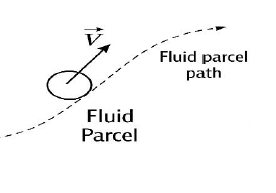
\includegraphics[width=\textwidth]{figures/figure1_2.png}
        \subcaption{Description lagrangienne}
        \label{fig:lagrangienne}
    \end{minipage}
    \hfill
    \begin{minipage}{0.45\textwidth}
        \centering
        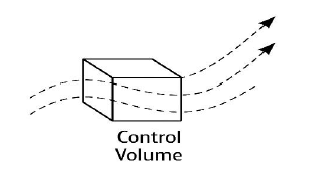
\includegraphics[width=\textwidth]{figures/figure1_3.png}
        \subcaption{Description eulérienne}
        \label{fig:eulerienne}
    \end{minipage}
    \caption{Représentations des approches lagrangienne et eulérienne en mécanique des fluides.}
    \label{fig:approches_lagrangienne_eulerienne}
\end{figure}

\subsection{L'équation de continuité}
\label{subsec:continuite}

L'équation de continuité traduit le principe de conservation de la masse, stipulant que le taux de changement de la masse du système dans le temps est nul \cite{batchelor1967introduction}. Pour un volume de contrôle fixe, la forme intégrale s'écrit :

\begin{equation}
\frac{\partial}{\partial t} \int_{V_c} \rho \, d\Omega + \int_{S_c} \rho \, \vec{V} \cdot \vec{n} \, dS = 0
\label{eq:continuite_integrale}
\end{equation}
\begin{itemize}
    \item[--] \(t\) : le temps
    \item[--] \(V_c\) : le volume de contrôle
    \item[--] \(\rho\) : la masse volumique du fluide \([kg/m^3]\)
    \item[--] \(\Omega\) : le domaine du volume de contrôle
    \item[--] \(S_c\) : la surface de contrôle (frontière du volume de contrôle)
    \item[--] \(\vec{V}\) : le vecteur vitesse du fluide \([m/s]\)
    \item[--] \(\vec{n}\) : le vecteur unitaire normal à la surface \(S_c\), orienté vers l'extérieur
\end{itemize}

Cette équation indique que la somme de la variation temporelle de la masse contenue dans le volume de contrôle et du flux massique à travers sa surface est nulle, comme illustré par le volume de contrôle fixe représenté à la Figure~\ref{fig:volume_controle_fixe}. Par application de la formule de divergence sur un volume élémentaire infinitésimal (Figure~\ref{fig:volume_elementaire}), on obtient la forme locale de l'équation de continuité : \cite{panton2013incompressible}

\begin{equation}
\frac{\partial \rho}{\partial t} + \nabla \cdot (\rho \vec{V}) = 0
\label{eq:continuite_locale}
\end{equation}

Pour un fluide incompressible, hypothèse valable pour l'eau dans la plupart des applications hydrauliques, la masse volumique reste constante, ce qui simplifie l'équation à :

\begin{equation}
\nabla \cdot \vec{V} = 0
\label{eq:continuite_incompressible}
\end{equation}

\begin{figure}[H]
    \centering
    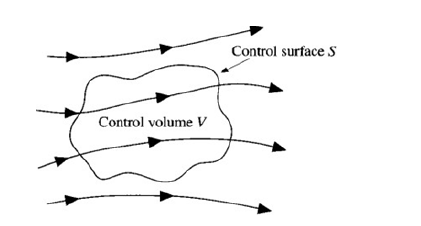
\includegraphics[width=0.6\textwidth]{figures/figure1_4.png}
    \caption{Volume de contrôle fixe traversé par le fluide en mouvement.}
    \label{fig:volume_controle_fixe}
\end{figure}

\begin{figure}[H]
    \centering
    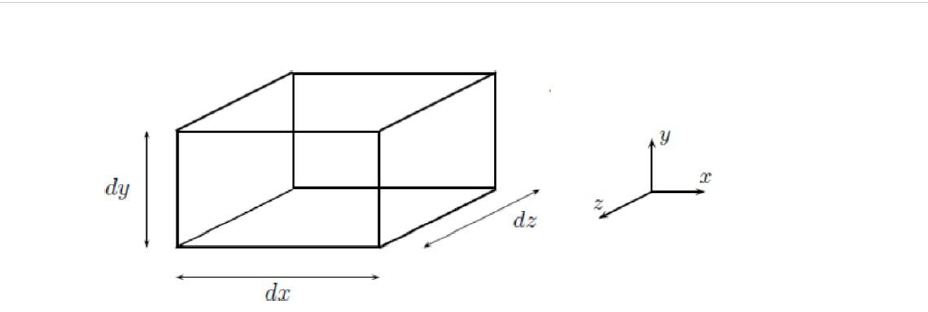
\includegraphics[width=0.6\textwidth]{figures/figure1_5.png}
    \caption{Volume élémentaire fixe pour l'établissement de la forme locale.}
    \label{fig:volume_elementaire}
\end{figure}

\subsection{L'équation de conservation de la quantité de mouvement}
\label{subsec:quantite_mouvement}

La conservation de la quantité de mouvement découle de l'application de la seconde loi de Newton à un élément fluide. Elle stipule que le taux de variation de la quantité de mouvement est égal à la somme des forces extérieures (forces de volume et forces de surface) \cite{currie2012fundamental}.

\begin{figure}[H]
    \centering
    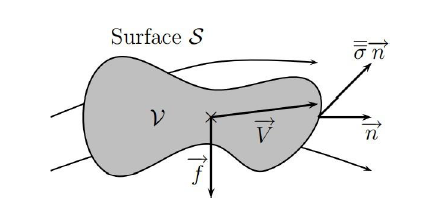
\includegraphics[width=0.6\textwidth]{figures/figure1_6.png}
    \caption{Volume de contrôle en mouvement sur lequel s'appliquent des efforts.}
    \label{fig:volume_controle_mouvement}
\end{figure}

Pour un fluide newtonien incompressible, les équations de Navier-Stokes s'écrivent sous forme vectorielle :

\begin{equation}
\rho \left( \frac{\partial \vec{V}}{\partial t} + (\vec{V} \cdot \nabla)\vec{V} \right) = -\nabla p + \mu \nabla^2 \vec{V} + \rho \vec{f}
\label{eq:navier_stokes}
\end{equation}

où les termes non encore définis précédemment sont :
\begin{itemize}
    \item[--] \(p\) : la pression statique du fluide \([Pa]\)
    \item[--] \(\mu\) : la viscosité dynamique du fluide \([Pa \cdot s]\)
    \item[--] \(\vec{f}\) : le vecteur des forces de volume (par unité de masse, typiquement la pesanteur \(\vec{g}\)) \([m/s^2]\)
    \item[--] \(\nabla p\) : le gradient de pression (force de pression par unité de volume)
    \item[--] \(\mu \nabla^2 \vec{V}\) : le terme de diffusion visqueuse (forces visqueuses par unité de volume)
\end{itemize}

Cette équation comporte deux termes fondamentaux :
\begin{itemize}
    \item Le \textbf{terme de convection} \( (\vec{V} \cdot \nabla)\vec{V} \), source de non-linéarité et de complexité. \item Le \textbf{terme de diffusion} \( \mu \nabla^2 \vec{V} \), représentant les interactions moléculaires dissipatives \cite{white2015fluid}. \end{itemize}

Les équations \eqref{eq:continuite_incompressible} et \eqref{eq:navier_stokes} forment un système de quatre équations aux dérivées partielles pour quatre inconnues (pression $p$ et les trois composantes de vitesse). Bien que mathématiquement bien posé, ce système ne possède pas de solution analytique générale en raison de sa non-linéarité \cite{kundu2015fluid}.

\section{Avantages de la CFD par rapport aux études expérimentales}
\label{sec:avantages_cfd}

Les récents progrès de la CFD en font un outil intéressant surtout en termes de coûts et de temps par rapport aux études expérimentales, dans un grand nombre de domaines de l'ingénierie, que ce soit dans l'industrie ou au niveau académique \cite{wendt2009computational}. Les différents avantages de la CFD par rapport aux essais expérimentaux en laboratoire sont résumés dans le tableau ci-dessous : \cite{roychowdhury2020computational}

\begin{table}[H]
    \centering
    \caption{Comparaison entre la CFD et les études expérimentales}
    \label{tab:comparaison_cfd_exp}
    \begin{tabular}{|l|c|c|}
        \hline
        \textbf{Critère} & \textbf{CFD} & \textbf{Études Expérimentales} \\
        \hline
        Coûts & Relativement bon marché & Cher \\
        \hline
        Temps & Court & Long \\
        \hline
        Échelles & Toutes (modèle réel possible) & Petites/Moyennes (modèles réduits) \\
        \hline
        Informations & Accès à toutes les variables en tout point & Limitée aux points de mesure \\
        \hline
        Répétabilité & Sans limite et parfaitement contrôlable & Difficile à cause des incertitudes \\
        \hline
        Sécurité & Très sécuritaire & Peut-être dangereux \\
        \hline
        Analyse de scénarios & Très simple et rapide & Lourd et coûteux \\
        \hline
    \end{tabular}
\end{table}

\section{Conclusion}
\label{sec:conclusion_chap1}

Ce premier chapitre a établi les fondements théoriques de la mécanique des fluides numérique, en présentant les équations de conservation qui constituent le socle de toute simulation CFD. La compréhension de ces équations est essentielle pour appréhender les défis liés à la modélisation des écoulements, notamment le caractère non-linéaire des équations de Navier-Stokes qui rend leur résolution analytique impossible dans le cas général. Cette situation justifie pleinement le recours aux méthodes numériques développées dans les chapitres suivants.
% ============================================================
%  CHAPITRE 2 : La turbulence en mécanique des fluides numérique
% ============================================================
\chapter{La turbulence en mécanique des fluides numérique}
\label{chap:turbulence}

\section{Introduction}
\label{sec:introduction_turbulence}

La turbulence désigne l'état de l'écoulement d'un fluide, liquide ou gaz, dont la vitesse possède un caractère tourbillonnaire et une orientation variable constamment dans l'espace, ce qui ne permet pas de prévoir son comportement de manière déterministe \cite{tennekes1972first}. Les écoulements turbulents se caractérisent par :
\begin{itemize}
    \item Le désordre et l'irrégularité de l'écoulement. \item Un caractère tridimensionnel et non-linéaire. \item La présence de tourbillons de différentes échelles avec un transfert d'énergie des plus grands vers les plus petits \cite{pope2000turbulent}, comme illustré à la Figure~\ref{fig:turbulent}. \end{itemize}

\begin{figure}[H]
    \centering
    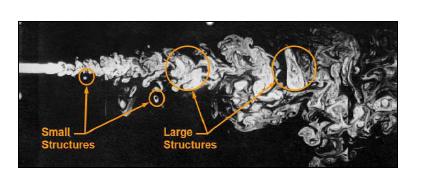
\includegraphics[width=0.45\textwidth]{figures/figure2_2.png}
    \caption{Écoulement turbulent.}
    \label{fig:turbulent}
\end{figure}

L'origine du désordre caractérisant l'écoulement repose sur le terme non-linéaire de l'équation de Navier-Stokes qui est le terme inertiel de transport par convection. Ainsi, plus le nombre de Reynolds est grand, plus ce terme aura du poids dans la dynamique et plus l'écoulement sera complexe et turbulent \cite{davidson2015turbulence}. Le nombre de Reynolds est donné comme suit : \cite{reynolds1883experimental}

\begin{equation}
Re = \frac{V \times L}{\nu}
\label{eq:reynolds}
\end{equation}

\begin{itemize}
    \item[--] \(V\) : la vitesse caractéristique de l'écoulement \([m/s]\)
    \item[--] \(L\) : la longueur caractéristique du domaine \([m]\)
    \item[--] \(\nu\) : la viscosité cinématique du fluide \([m^2/s]\)
\end{itemize}

Le tableau ci-dessous illustre, à titre d'exemple, quelques valeurs critiques de $Re$ pour différentes géométries :

\begin{table}[H]
    \centering
    \caption{Exemples de valeurs critiques du nombre de Reynolds}
    \label{tab:reynolds_critique}
    \begin{tabular}{|l|c|c|}
        \hline
        \textbf{Géométrie} & \textbf{Longueur caractéristique L} & \textbf{Re critique} \\
        \hline
        Écoulement en conduite & Diamètre (D) & $\approx 2300$ \\
        \hline
        Plaque plane (couche limite) & Longueur de la plaque (x) & $\approx 5\times10^5$ \\
        \hline
        Écoulement autour d'une sphère & Diamètre (D) & $\approx 3\times10^5$ \\
        \hline
        Entre deux plaques parallèles & Distance entre plaques (h) & $\approx 1000$ \\
        \hline
    \end{tabular}
\end{table}

\section{Les approches de modélisation de la turbulence}
\label{sec:approches_turbulence}

La modélisation de la turbulence est une branche de la mécanique des fluides utilisée pour prédire le comportement d'un écoulement dans lequel tout ou partie du fluide est turbulent. Malgré des efforts importants de recherche depuis plus d'un siècle, la modélisation des écoulements turbulents demeure un défi à relever \cite{wilcox2006turbulence}. Il existe principalement trois axes de recherche : \cite{sagaut2006large}

\subsection{Simulation numérique directe (DNS)}
\label{subsec:dns}

La DNS permet de résoudre directement les équations de Navier-Stokes (voir équation~\eqref{eq:navier_stokes}) sans aucune modélisation. Elle présente ainsi l'avantage de donner accès à toutes les quantités instantanées considérées dans l'écoulement. Tous les mouvements doivent être résolus depuis les plus petites échelles dissipatives jusqu'à l'échelle intégrale, comme illustré à la Figure~\ref{fig:dns_jet}. Le nombre de mailles est alors très important, ce qui engendre des temps de calcul extrêmement longs \cite{moin1998direct}. La capacité et la performance des calculateurs actuels ne cessent de progresser mais ne permettent pas encore de sonder des écoulements complexes dans un contexte industriel.

\begin{figure}[H]
    \centering
    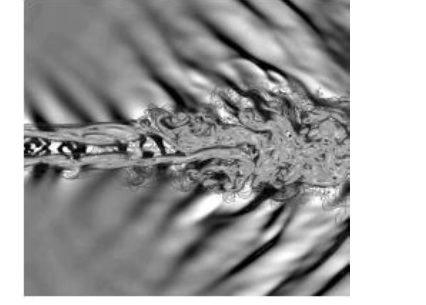
\includegraphics[width=0.6\textwidth]{figures/figure2_3.png}
    \caption{DNS d'un jet d'air issu d'une tuyère \cite{moin1998direct}.}
    \label{fig:dns_jet}
\end{figure}

\subsection{Simulation des grandes échelles (LES~: Large Eddy Simulation)}
\label{subsec:les}

La LES est une méthode numérique intermédiaire entre la DNS et les méthodes statistiques \cite{lesieur2005large}. Elle consiste à appliquer un filtre spatial aux équations de Navier-Stokes (voir équation~\eqref{eq:navier_stokes}) en tout point du domaine. Le champ filtré est défini par :

\begin{equation}
\bar{\Phi}(x) = \int_D \Phi(x') G(x, x') dx'
\label{eq:filtre_les}
\end{equation}

\begin{itemize}
    \item[--] \(\bar{\Phi}(x)\) : le champ filtré (représentant les grandes échelles)
    \item[--] \(\Phi(x')\) : le champ instantané non filtré
    \item[--] \(G(x, x')\) : le noyau (fonction) du filtre spatial
    \item[--] \(D\) : le domaine de filtrage
\end{itemize}

Le filtre sépare les grandes échelles (simulées) des petites structures (modélisées), comme illustré à la Figure~\ref{fig:les_anneaux}. On suppose ici que le comportement de ces dernières ne dépend pas de la géométrie et est universel. La LES est moins coûteuse que la DNS, mais reste très exigeante en ressources de calcul, ce qui limite encore son application industrielle courante \cite{piomelli1999large}.

\begin{figure}[H]
    \centering
    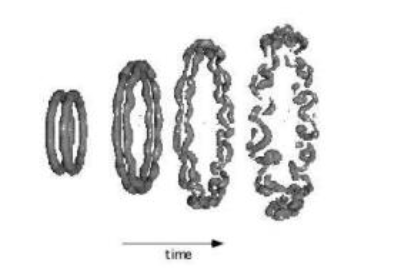
\includegraphics[width=0.6\textwidth]{figures/figure2_4.png}
    \caption{LES de la collision axiale de deux anneaux tourbillonnaires \cite{piomelli1999large}.}
    \label{fig:les_anneaux}
\end{figure}

\subsection{Modélisation statistique (RANS)}
\label{subsec:rans}

La méthode RANS (Reynolds-Averaged Navier-Stokes) est une approche qui consiste à mettre de côté le mouvement instantané du fluide, afin d'exprimer les équations du champ moyen en se servant de la décomposition de Reynolds. Chaque variable est décomposée en une partie moyenne et une partie fluctuante \cite{reynolds1895dynamical} :

\begin{equation}
\phi(x_i, t) = \overline{\phi}(x_i) + \phi'(x_i, t)
\label{eq:decomposition_reynolds}
\end{equation}

\begin{figure}[H]
    \centering
    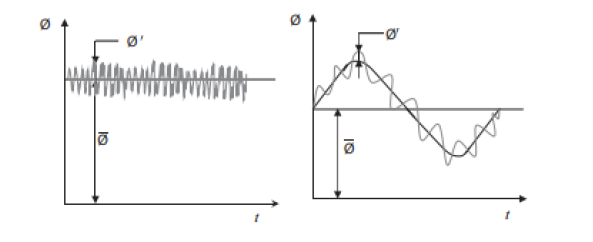
\includegraphics[width=0.6\textwidth]{figures/figure2_5.png}
    \caption{Décomposition des variables selon l'approche RANS \cite{reynolds1895dynamical}.}
    \label{fig:decomposition_reynolds}
\end{figure}

En introduisant cette décomposition dans les équations de Navier-Stokes et en prenant la moyenne, on obtient les équations RANS (Reynolds-Averaged Navier-Stokes), dont le principe est illustré à la Figure~\ref{fig:decomposition_reynolds}. Ce processus fait apparaître de nouvelles inconnues : les \textbf{tensions de Reynolds} (\( -\rho \overline{u_i' u_j'} \)), qui représentent l'influence des fluctuations turbulentes sur l'écoulement moyen \cite{hinze1975turbulence}.

\subsection{Remarques sur les trois approches}
\label{subsec:remarques_approches}

Pour une modélisation précise, il faut prévoir des maillages très fins, ce qui nécessite des coûts et des temps très importants. C'est pour cela qu'on préfère l'approche statistique car elle est plus rapide et moins coûteuse \cite{rodi1993turbulence}. Le tableau suivant compare les différentes approches de modélisation : \cite{durbin2010statistical}

\begin{table}[H]
    \centering
    \caption{Comparaison des approches de modélisation de la turbulence}
    \label{tab:comparaison_approches}
    \small
    \begin{tabular}{|l|p{3.5cm}|p{2.5cm}|p{1.8cm}|p{3.5cm}|}
        \hline
        \textbf{Approche} & \textbf{Résolution des tourbillons} & \textbf{Coût de calcul} & \textbf{Précision} & \textbf{Applications} \\
        \hline
        RANS & Tous modélisés & Faible & Moyenne & Industrielles courantes \\
        \hline
        LES & Grands résolus, petits modélisés & Élevé & Bonne & Recherche, écoulements complexes \\
        \hline
        DNS & Tous résolus & Extrêmement élevé & Excellente & Recherche fondamentale \\
        \hline
    \end{tabular}
\end{table}

\section{Classification des modèles de turbulence}
\label{sec:classification_modeles}

Le système formé par les équations RANS n'est pas fermé, car on dispose de quatre équations mais dix inconnues, ce sont les tensions de Reynolds qui posent le problème. L'enjeu est de trouver une relation liant les tensions de Reynolds au champ de vitesse moyen \cite{launder1972lectures}.

\subsection{Modèle à viscosité turbulente}
\label{subsec:viscosite_turbulente}

Boussinesq fut le premier à introduire la notion de viscosité turbulente en proposant une relation en analogie avec celle de Newton pour les contraintes de viscosité moléculaire \cite{boussinesq1877essai}. Schématiquement cela revient à poser une relation linéaire entre les contraintes turbulentes (contraintes de Reynolds) et le gradient de vitesse moyen : \cite{schmitt2007boussinesq}

\begin{equation}
-\rho \overline{u_i' u_j'} = \mu_t \left( \frac{\partial \overline{u_i}}{\partial x_j} + \frac{\partial \overline{u_j}}{\partial x_i} \right) - \frac{2}{3} \rho k \delta_{ij}
\label{eq:boussinesq}
\end{equation}

où les termes sont définis comme suit :
\begin{itemize}
    \item[--] \(\mu_t\) : la viscosité dynamique turbulente \([Pa \cdot s]\)
    \item[--] \(k\) : l'énergie cinétique turbulente \([m^2/s^2]\)
    \item[--] \(\delta_{ij}\) : le tenseur de Kronecker (\(\delta_{ij} = 1\) si \(i=j\), 0 sinon)
    \item[--] \(\overline{u_i}\), \(\overline{u_j}\) : les composantes de la vitesse moyenne
\end{itemize}

\subsection{Le modèle de longueur de mélange -- modèle de Prandtl}
\label{subsec:longueur_melange}

Une étude dimensionnelle montre que la viscosité turbulente est proportionnelle à une échelle de longueur $l$ et une échelle de vitesse $u$ représentatives de l'agitation turbulente \cite{prandtl1925bericht}. Prandtl a proposé le modèle de longueur de mélange dans lequel la viscosité cinématique turbulente \( \nu_t \) est directement reliée au gradient de vitesse moyenne par l'intermédiaire d'une longueur \( l_m \) appelée longueur de mélange : \cite{prandtl1945uber}

\begin{equation}
\nu_t = l_m^2 \left| \frac{\partial \bar{u}}{\partial y} \right|
\label{eq:longueur_melange}
\end{equation}

Avec \( l_m = \kappa y \) et \( \kappa = 0{,}41 \) la constante de Von Karman.

\section{Modèles de fermeture des approches statistiques à deux équations de transport}
\label{sec:modeles_deux_equations}

Plusieurs modèles à deux équations ont été développés pour représenter les deux échelles indépendamment. Ils sont largement utilisés dans l'industrie \cite{hanjalic2011modelling}.

\subsection{Modèle de fermeture \texorpdfstring{$k$-$\varepsilon$}{k-epsilon}}
\label{subsec:modele_k_epsilon}

Ce modèle a été établi par Jones et Launder \cite{jones1972prediction}. Il relie les grandeurs caractéristiques de la turbulence : énergie cinétique turbulente $k$, taux de dissipation $\varepsilon$ et viscosité turbulente \( \mu_t \). Les équations de transport de $k$ et $\varepsilon$ sont \cite{launder1974application} :

\begin{align}
\frac{\partial}{\partial t} (\rho k) + \frac{\partial}{\partial x_j} (\rho u_j k) &= \frac{\partial}{\partial x_j} \left[ \left( \mu + \frac{\mu_t}{\sigma_k} \right) \frac{\partial k}{\partial x_j} \right] + P_k - \rho \varepsilon \label{eq:transport_k} \\
\frac{\partial}{\partial t} (\rho \varepsilon) + \frac{\partial}{\partial x_j} (\rho u_j \varepsilon) &= \frac{\partial}{\partial x_j} \left[ \left( \mu + \frac{\mu_t}{\sigma_\varepsilon} \right) \frac{\partial \varepsilon}{\partial x_j} \right] + C_{\varepsilon 1} \frac{\varepsilon}{k} P_k - C_{\varepsilon 2} \frac{\rho \varepsilon^2}{k} \label{eq:transport_epsilon}
\end{align}

La viscosité turbulente est donnée par \( \mu_t = \rho C_\mu \frac{k^2}{\varepsilon} \). Les constantes du modèle standard sont : \( C_\mu = 0,09 \), \( C_{\varepsilon 1} = 1,44 \), \( C_{\varepsilon 2} = 1,92 \), \( \sigma_k = 1,0 \), \( \sigma_\varepsilon = 1,3 \) \cite{launder1974numerical}.

\subsection{Modèle de fermeture \( k-\omega \)}
\label{subsec:modele_k_omega}

Le modèle \( k-\omega \) de Wilcox \cite{wilcox1988reassessment} utilise le paramètre \( \omega \), le taux de dissipation spécifique défini par \( \omega = \varepsilon/k \). La viscosité turbulente devient \( \mu_t = \rho \frac{k}{\omega} \). Les équations de transport sont \cite{wilcox2008formulation} :

\begin{align}
\frac{\partial}{\partial t} (\rho k) + \frac{\partial}{\partial x_j} (\rho u_j k) &= \frac{\partial}{\partial x_j} \left[ \left( \mu + \frac{\mu_t}{\sigma_k} \right) \frac{\partial k}{\partial x_j} \right] + P_k - \beta^* \rho k \omega \label{eq:transport_k_omega} \\
\frac{\partial}{\partial t} (\rho \omega) + \frac{\partial}{\partial x_j} (\rho u_j \omega) &= \frac{\partial}{\partial x_j} \left[ \left( \mu + \frac{\mu_t}{\sigma_\omega} \right) \frac{\partial \omega}{\partial x_j} \right] + \alpha \frac{\omega}{k} P_k - \beta \rho \omega^2 \label{eq:transport_omega}
\end{align}

\subsection{Modèle de fermeture \( k-\omega \) SST}
\label{subsec:modele_k_omega_sst}

Menter \cite{menter1994two} a proposé un modèle hybride combinant les avantages des modèles \( k-\omega \) près des parois et \( k-\varepsilon \) loin des parois. Le modèle \( k-\omega \) SST (Shear Stress Transport) utilise une fonction de commutation \( F_1 \) pour basculer entre les deux formulations \cite{menter2003ten} :

\begin{equation}
\mu_t = \frac{a_1 \rho k}{\max(a_1 \omega, S F_2)}
\label{eq:mu_t_sst}
\end{equation}

\begin{itemize}
    \item[--] \(a_1 = 0{,}31\) : constante du modèle SST
    \item[--] \(\rho\) : masse volumique du fluide \([kg/m^3]\)
    \item[--] \(k\) : énergie cinétique turbulente \([m^2/s^2]\)
    \item[--] \(\omega\) : taux de dissipation spécifique \([1/s]\)
    \item[--] \(S\) : invariant du tenseur des taux de déformation \([1/s]\)
    \item[--] \(F_2\) : seconde fonction de commutation du modèle SST
\end{itemize}

Ce modèle sera privilégié pour notre étude car il offre une bonne précision dans les zones à forts gradients de vitesse, ce qui est essentiel pour modéliser correctement les écoulements dans les évacuateurs de crues et les vidanges de fond.


% SECTION 2.5 : CONCLUSION
\section{Conclusion}
\label{sec:conclusion_chap2}

En définitive, bien que la turbulence soit un phénomène omniprésent dans la nature et le quotidien, elle reste difficile à définir avec précision en raison de son caractère chaotique et imprévisible. Ce comportement tourbillonnaire, en perpétuelle variation de forme, de position et d'intensité, traduit la complexité du régime turbulent. Pour notre étude, le modèle \( k-\omega \) SST sera privilégié car il combine robustesse et précision.
% ============================================================
%  CHAPITRE 3 : Approximations numériques pour la résolution des EDP
% ============================================================
\chapter{Approximations numériques pour la résolution des équations aux dérivées partielles}
\label{chap:approximations_numeriques}

\section{Introduction}
\label{sec:introduction_approx}

Les équations de Navier-Stokes sont largement utilisées pour modéliser le comportement des fluides. Toutefois, en tant qu'équations aux dérivées partielles (EDP) non linéaires, elles ne disposent pas de solution analytique générale. Pour cette raison, la résolution numérique constitue l'approche privilégiée afin d'obtenir des solutions approchées \cite{hirsch2007numerical}.

Parmi les techniques numériques les plus courantes, les méthodes des différences finies, des volumes finis et des éléments finis permettent de discrétiser le problème continu en un système algébrique traitable \cite{tannehill1997computational}.

\section{Méthode des différences finies}
\label{sec:differences_finies}

La méthode des différences finies consiste à approximer les dérivées des équations physiques à l'aide des séries de Taylor, en s'appuyant directement sur la définition mathématique de la dérivée \cite{smith1985numerical}.

\begin{figure}[H]
    \centering
    \begin{tikzpicture}[scale=1.15]
      % Axes
      \draw[->] (-0.3,0) -- (5.3,0) node[right] {$X$};
      \draw[->] (0,-0.3) -- (0,3.8) node[above] {$t$};
      \node[left, font=\small] at (-0.05,3.5) {$\tau$};
      % Positions x
      \def\xa{1.0} \def\xb{2.5} \def\xc{4.0}
      % Positions t
      \def\ta{1.0} \def\tb{2.7}
      % Lignes de grille verticales
      \draw[gray!60, dashed] (\xa,0) -- (\xa,3.4);
      \draw[gray!60, dashed] (\xb,0) -- (\xb,3.4);
      \draw[gray!60, dashed] (\xc,0) -- (\xc,3.4);
      % Lignes de grille horizontales
      \draw[gray!60, dashed] (0,\ta) -- (5.0,\ta);
      \draw[gray!60, dashed] (0,\tb) -- (5.0,\tb);
      % Étiquettes axe x
      \node[below, font=\small] at (\xa,0) {$x_{i-1}$};
      \node[below, font=\small] at (\xb,0) {$x_i$};
      \node[below, font=\small] at (\xc,0) {$x_{i+1}$};
      \node[below, font=\small] at (5.0,0) {$L$};
      \node[below left, font=\small] at (0,0) {$0$};
      % Étiquettes axe t
      \node[left, font=\small] at (0,\ta) {$t^n$};
      \node[left, font=\small] at (0,\tb) {$t^{n+1}$};
      % Points à t^n
      \fill (\xa,\ta) circle (4pt);
      \fill (\xb,\ta) circle (4pt);
      \fill (\xc,\ta) circle (4pt);
      % Points à t^{n+1}
      \fill (\xb,\tb) circle (4pt);
      \draw[fill=white] (\xa,\tb) circle (4pt);
      \draw[fill=white] (\xc,\tb) circle (4pt);
      % Étiquettes des n\oe uds
      \node[above right, font=\scriptsize] at (\xa,\ta) {$u_{i-1}^n$};
      \node[above right, font=\scriptsize] at (\xb,\ta) {$u_i^n$};
      \node[above right, font=\scriptsize] at (\xc,\ta) {$u_{i+1}^n$};
      \node[above right, font=\scriptsize] at (\xb,\tb) {$u_i^{n+1}$};
      % Annotation \Delta x
      \draw[<->] (\xa,0.45) -- (\xb,0.45) node[midway, above, font=\scriptsize] {$\Delta x$};
      % Annotation \Delta t
      \draw[<->] (4.6,\ta) -- (4.6,\tb) node[midway, right, font=\scriptsize] {$\Delta t$};
    \end{tikzpicture}
    \caption{Maillage de la méthode des différences finies.}
    \label{fig:maillage_df}
\end{figure}

Pour une fonction $u(x)$, la dérivée première peut être approximée par différents schémas. En utilisant le développement en série de Taylor :

\begin{equation}
u(x + \Delta x) = u(x) + \Delta x \frac{\partial u}{\partial x} + \frac{\Delta x^2}{2} \frac{\partial^2 u}{\partial x^2} + \dots
\label{eq:taylor}
\end{equation}

On obtient :
\begin{itemize}
    \item \textbf{Schéma décentré avant} (ordre 1) : \( \left( \frac{\partial u}{\partial x} \right)_i \approx \frac{u_{i+1} - u_i}{\Delta x} \)
    \item \textbf{Schéma décentré arrière} (ordre 1) : \( \left( \frac{\partial u}{\partial x} \right)_i \approx \frac{u_i - u_{i-1}}{\Delta x} \)
    \item \textbf{Schéma centré} (ordre 2) : \( \left( \frac{\partial u}{\partial x} \right)_i \approx \frac{u_{i+1} - u_{i-1}}{2\Delta x} \)
\end{itemize}

La dérivée seconde est approximée par le schéma centré d'ordre 2 \cite{strikwerda2004finite} :

\begin{equation}
\left( \frac{\partial^2 u}{\partial x^2} \right)_i \approx \frac{u_{i+1} - 2u_i + u_{i-1}}{\Delta x^2}
\label{eq:derivee_seconde}
\end{equation}

\section{Méthode des éléments finis}
\label{sec:elements_finis}

La méthode des éléments finis vise à minimiser l'erreur générée lors de l'approximation d'un problème continu par sa formulation discrète \cite{zienkiewicz2013finite}. Le domaine est subdivisé en petits éléments de géométrie simple interconnectés en des points appelés "nœuds". La solution est recherchée sous forme d'une combinaison linéaire de fonctions de base locales \cite{reddy2006introduction} :

\begin{equation}
\Phi_h(x) = \sum_{i=1}^{n} \Phi_i(x)\, N_i
\label{eq:elements_finis}
\end{equation}

\begin{itemize}
    \item[--] \(\Phi_h(x)\) : solution approchée discrète sur le domaine
    \item[--] \(\Phi_i(x)\) : valeur nodale de la solution au n\oe ud \(i\)
    \item[--] \(N_i\) : fonction de forme (base) associée au n\oe ud \(i\)
    \item[--] \(n\) : nombre total de n\oe uds de l'élément
\end{itemize}

Cette méthode est très mathématique et peut être appliquée à des géométries variées, mais elle rencontre des obstacles lorsqu'il s'agit de termes non linéaires, ce qui limite son application en CFD \cite{hughes2012finite}.

\begin{figure}[H]
    \centering
    \begin{tikzpicture}[scale=0.95]
      % Triangle 3 n\oe uds
      \begin{scope}[xshift=0cm]
        \draw[thick] (0,0) -- (1.4,0) -- (0.7,1.2) -- cycle;
        \fill (0,0) circle (3pt); \fill (1.4,0) circle (3pt); \fill (0.7,1.2) circle (3pt);
        \node[below, font=\footnotesize, align=center] at (0.7,-0.4) {Triangle\\3 n\oe uds};
      \end{scope}
      % Triangle 6 n\oe uds
      \begin{scope}[xshift=2.6cm]
        \draw[thick] (0,0) -- (1.4,0) -- (0.7,1.2) -- cycle;
        \fill (0,0) circle (3pt); \fill (1.4,0) circle (3pt); \fill (0.7,1.2) circle (3pt);
        \fill (0.7,0) circle (3pt); \fill (1.05,0.6) circle (3pt); \fill (0.35,0.6) circle (3pt);
        \node[below, font=\footnotesize, align=center] at (0.7,-0.4) {Triangle\\6 n\oe uds};
      \end{scope}
      % Quadrilat\`ere 4 n\oe uds
      \begin{scope}[xshift=5.2cm]
        \draw[thick] (0,0) -- (1.4,0) -- (1.4,1.2) -- (0,1.2) -- cycle;
        \fill (0,0) circle (3pt); \fill (1.4,0) circle (3pt);
        \fill (1.4,1.2) circle (3pt); \fill (0,1.2) circle (3pt);
        \node[below, font=\footnotesize, align=center] at (0.7,-0.4) {Quadrilat\`ere\\4 n\oe uds};
      \end{scope}
      % Quadrilat\`ere 8 n\oe uds
      \begin{scope}[xshift=7.8cm]
        \draw[thick] (0,0) -- (1.4,0) -- (1.4,1.2) -- (0,1.2) -- cycle;
        \fill (0,0) circle (3pt); \fill (0.7,0) circle (3pt); \fill (1.4,0) circle (3pt);
        \fill (1.4,0.6) circle (3pt); \fill (1.4,1.2) circle (3pt);
        \fill (0.7,1.2) circle (3pt); \fill (0,1.2) circle (3pt); \fill (0,0.6) circle (3pt);
        \node[below, font=\footnotesize, align=center] at (0.7,-0.4) {Quadrilat\`ere\\8 n\oe uds};
      \end{scope}
    \end{tikzpicture}
    \caption{Les géométries de référence de quelques éléments 2D courants.}
    \label{fig:elements_2d}
\end{figure}

\begin{figure}[H]
    \centering
    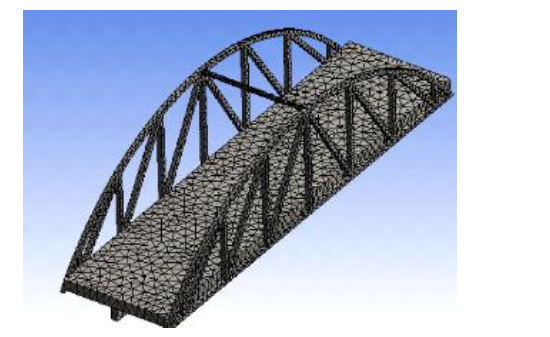
\includegraphics[width=0.6\textwidth]{figures/figure3_3.png}
    \caption{Maillage en éléments finis d'un pont de type Bow-string en vue d'une simulation.}
    \label{fig:maillage_pont}
\end{figure}

\section{Méthode des volumes finis}
\label{sec:volumes_finis}

La méthode des volumes finis repose sur l'intégration des équations en formulation intégrale sur des volumes élémentaires \cite{leveque2002finite}. Contrairement à la méthode des éléments finis, elle est particulièrement bien adaptée à la discrétisation spatiale des lois de conservation, ce qui en fait une méthode de choix en mécanique des fluides \cite{eymard2000finite}.

L'équation générale de transport pour une variable \( \phi \) s'écrit sous forme conservative \cite{moukalled2016finite} :

\begin{equation}
\frac{\partial}{\partial t}(\rho\phi) + \nabla\cdot(\rho\phi\vec{u}) = \nabla\cdot(\Gamma\nabla\phi) + S_\phi
\label{eq:transport_general}
\end{equation}

\begin{figure}[H]
    \centering
    \begin{tikzpicture}[scale=0.62]
      % --- (a) Cell-centred ---
      \begin{scope}[xshift=0cm]
        \draw[gray!70, thin] (0,0) grid (3,3);
        \fill[blue!15] (1,1) rectangle (2,2);
        \draw[blue, thick] (1,1) rectangle (2,2);
        \foreach \x in {0.5,1.5,2.5} {
          \foreach \y in {0.5,1.5,2.5} {
            \fill (\x,\y) circle (4pt);
          }}
        \node[below, font=\small] at (1.5,-0.5) {(a) \textit{Cell-centred}};
      \end{scope}
      % --- (b) Vertex-centred ---
      \begin{scope}[xshift=4.5cm]
        \draw[gray!70, thin] (0,0) grid (3,3);
        \fill[blue!15] (0.5,0.5) rectangle (1.5,1.5);
        \draw[blue, thick] (0.5,0.5) rectangle (1.5,1.5);
        \foreach \x in {0,1,2,3} {
          \foreach \y in {0,1,2,3} {
            \fill (\x,\y) circle (4pt);
          }}
        \node[below, font=\small] at (1.5,-0.5) {(b) \textit{Vertex-centred}};
      \end{scope}
      % --- (c) Cell-vertex ---
      \begin{scope}[xshift=9.0cm]
        \draw[gray!70, thin] (0,0) grid (3,3);
        % Un seul carré encadré par 4 noeuds voisins
        \fill[blue!20] (1,1) rectangle (2,2);
        \draw[blue, thick] (1,1) rectangle (2,2);
        % Points aux sommets (vertices)
        \foreach \x in {0,1,2,3} {
          \foreach \y in {0,1,2,3} {
            \fill (\x,\y) circle (4pt);
          }}
        \node[below, font=\small] at (1.5,-0.5) {(c) \textit{Cell-vertex}};
      \end{scope}
    \end{tikzpicture}
    \caption{Comparaison des approches (a) \og Cell-centred\fg{}, (b) \og Vertex-centred\fg{}, (c) \og Cell-vertex\fg{}.}
    \label{fig:approches_vf}
\end{figure}

\begin{figure}[H]
    \centering
    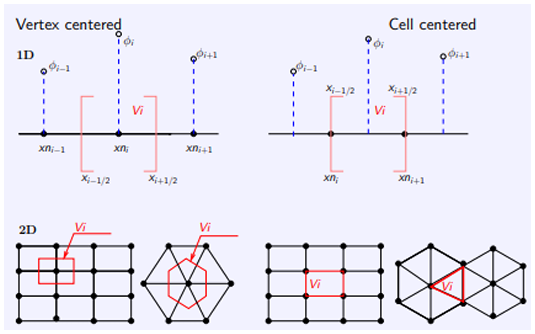
\includegraphics[width=0.6\textwidth]{figures/figure3_5.png}
    \caption{Exemples des volumes de contrôle en 1D et 2D.}
    \label{fig:volumes_controle_1d_2d}
\end{figure}

\begin{figure}[H]
    \centering
    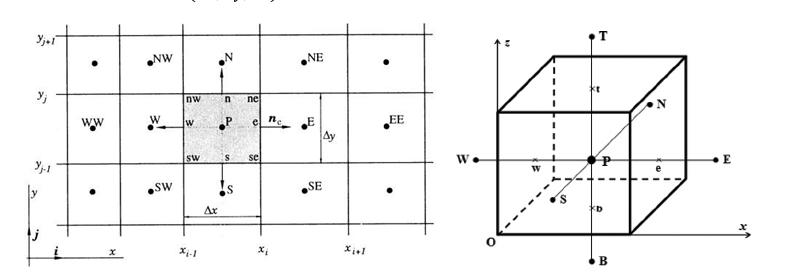
\includegraphics[width=0.6\textwidth]{figures/figure3_6.png}
    \caption{Exemple d'un volume de contrôle en 3D.}
    \label{fig:volume_controle_3d}
\end{figure}

\subsection{Discrétisation des termes de l'équation de transport}
\label{subsec:discretisation_termes}

\textbf{Discrétisation temporelle} : Le schéma d'Euler implicite, inconditionnellement stable mais précis au premier ordre, approxime la dérivée temporelle par \cite{butcher2016numerical} :

\begin{equation}
\int_V \frac{\partial (\rho\phi)}{\partial t} dV \approx \frac{(\rho\phi)_P^{n+1} - (\rho\phi)_P^n}{\Delta t} V_P
\label{eq:euler_implicite}
\end{equation}

\textbf{Terme de convection} : Il représente le transport de \( \phi \) par l'écoulement \cite{wesseling2001principles} :

\begin{equation}
\int_A \vec{n}\cdot(\rho\phi\vec{u})dA \approx \sum_f F_f \phi_f
\label{eq:convection}
\end{equation}

\textbf{Terme de diffusion} : Il représente le transport par gradient \cite{ferziger2002computational} :

\begin{equation}
\int_A \vec{n}\cdot(\Gamma\nabla\phi)dA \approx \sum_f \Gamma_f (\vec{n}\cdot\nabla\phi)_f A_f
\label{eq:diffusion}
\end{equation}

\subsection{Les schémas de discrétisation}
\label{subsec:schemas_discretisation}

\textbf{Schéma Upwind du premier ordre} : Stable et conservatif, ce schéma prend la valeur amont sans considération aval \cite{patankar1980numerical} :

\begin{equation}
\phi_e = \phi_P \text{ si } F_e > 0, \quad \phi_e = \phi_E \text{ si } F_e < 0
\label{eq:upwind}
\end{equation}

\begin{figure}[H]
    \centering
    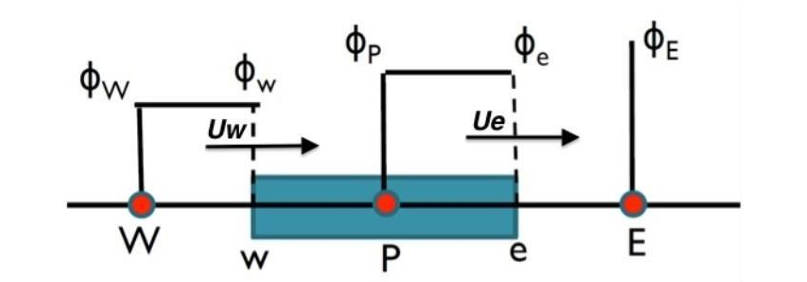
\includegraphics[width=0.6\textwidth]{figures/figure3_7.png}
    \caption{Schéma Upwind du 1er ordre.}
    \label{fig:upwind}
\end{figure}

\textbf{Schéma linéaire centré} : Plus précis (ordre 2), il utilise l'interpolation linéaire \cite{leonard1979stable} :

\begin{equation}
\phi_f = \frac{\phi_P + \phi_E}{2}
\label{eq:centre}
\end{equation}

\begin{figure}[H]
    \centering
    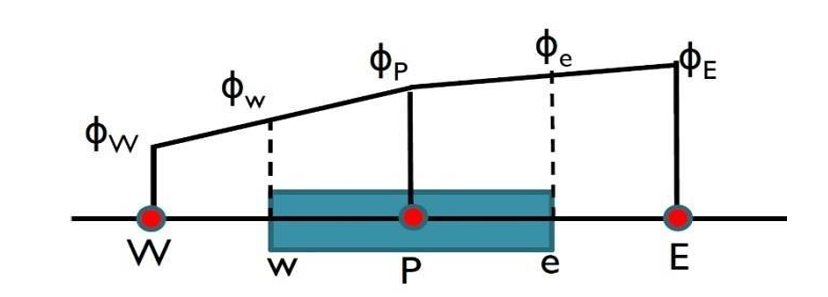
\includegraphics[width=0.6\textwidth]{figures/figure3_8.png}
    \caption{Schéma linéaire centré.}
    \label{fig:centre}
\end{figure}

\textbf{Schéma QUICK} : Proposé par Leonard \cite{leonard1991ultimate}, ce schéma d'ordre 3 utilise une interpolation quadratique pondérée :

\begin{equation}
\phi_e = \frac{6}{8}\phi_P + \frac{3}{8}\phi_E - \frac{1}{8}\phi_W \quad \text{pour } F_e > 0
\label{eq:quick}
\end{equation}

\begin{figure}[H]
    \centering
    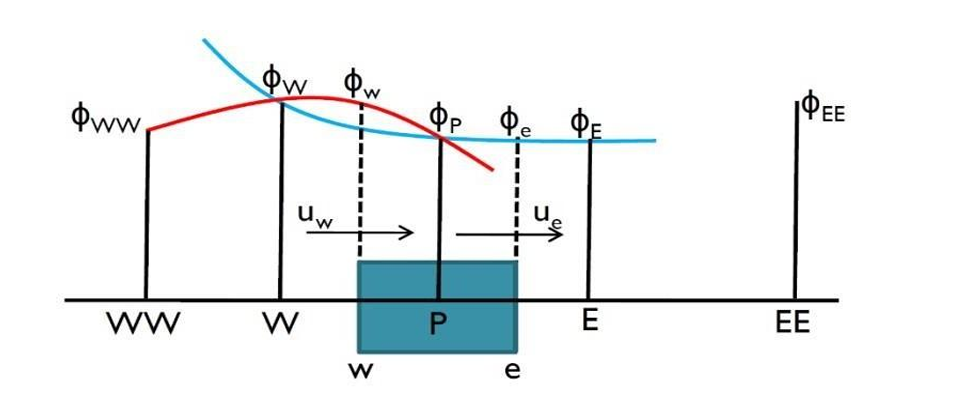
\includegraphics[width=0.6\textwidth]{figures/figure3_9.png}
    \caption{Schéma QUICK.}
    \label{fig:quick}
\end{figure}

\section{Conclusion}
\label{sec:conclusion_chap3}

Ce chapitre a introduit les diverses méthodes d'approximation numérique pour résoudre les équations de Navier-Stokes utilisées dans la modélisation hydraulique. Nous avons examiné les méthodes des différences finies, des éléments finis et des volumes finis. Ces méthodes constituent la base des outils de simulation numérique en hydraulique, et il est essentiel de choisir la méthode appropriée en fonction des caractéristiques du problème à résoudre. Dans notre cas, nous utiliserons la méthode des volumes finis qui est la méthode adoptée par OpenFOAM.

% ============================================================
%  CHAPITRE 4 : Présentation du barrage Ahl Souss (Ait M'zal)
% ============================================================
\chapter{Présentation du barrage Ahl Souss (Ait M'zal)}
\label{chap:barrage}

\section{Introduction}
\label{sec:introduction_barrage}

Le barrage Ahl Souss, également dénommé barrage Ait M'zal, s'inscrit dans le cadre du programme national des barrages visant à mobiliser les ressources en eau pour le développement socio-économique des régions. Cet ouvrage, dont la construction s'est achevée en 2005, constitue un aménagement hydraulique stratégique pour la province de Chtouka Ait Baha, répondant à des objectifs multiples d'alimentation en eau potable, d'irrigation et de recharge de la nappe phréatique \cite{scet1994ahl, fiche_historique}.

\section{Situation et accès}
\label{sec:situation_acces}

Le barrage Ait M'zal est implanté sur l'oued Izig, dans la commune rurale d'Ait M'zal, province de Chtouka Ait Baha, région administrative de Souss-Massa. Il se situe à proximité du douar Tlet Wanas, à environ 500 mètres de la route secondaire n°509, à 3,9 km du centre du village d'Ait Baha et à 65 km au sud-est d'Agadir \cite{scet1994ahl, fiche_synoptique}.

L'axe du barrage est défini par les points de coordonnées Lambert suivants \cite{fiche_synoptique} :
\begin{itemize}
    \item \textbf{Point A (rive droite)} : X = 140\,520,860 ; Y = 345\,215,940
    \item \textbf{Point B (rive gauche)} : X = 140\,516,280 ; Y = 345\,216,140
\end{itemize}

La cote moyenne du lit de l'oued au droit du barrage est de 572,00 NGM (Nivellement Général du Maroc). L'accès à l'ouvrage se fait par une route goudronnée de 3\,900 m depuis le village d'Ait Baha \cite{fiche_synoptique}.

\section{But de l'ouvrage}
\label{sec:but_ouvrage}

Conformément aux objectifs définis par l'Administration de l'Hydraulique, le barrage remplit trois fonctions principales \cite{scet1994ahl, fiche_synoptique} :
\begin{itemize}
    \item \textbf{L'irrigation} des périmètres agricoles situés en aval, contribuant à la sécurité alimentaire et au développement économique local.
    \item \textbf{L'alimentation en eau potable} des populations de la région, répondant aux besoins croissants liés à la démographie et au développement touristique.
    \item \textbf{La recharge de la nappe phréatique}, participant à la gestion durable des ressources en eau souterraines du bassin du Souss-Massa.
\end{itemize}

\section{Contexte géologique}
\label{sec:geologie}

La zone du barrage s'inscrit dans la partie nord de l'Anti-Atlas occidental, caractérisée par les formations du Précambrien I appartenant à la boutonnière de Kerdouss \cite{note_geologique_2003}. Le substratum est constitué de roches volcaniques acides.

La géologie de surface révèle des disparités entre les deux rives \cite{note_geologique_2003, fiche_synoptique} :
\begin{itemize}
    \item \textbf{Rive gauche} : présence de deux faciès :
    \begin{itemize}
        \item Une brèche volcanique blanchâtre à grisâtre à éléments grossiers, assez dure mais parfois friable, avec une résonance sourde aux coups du marteau.
        \item La roche est affectée par plusieurs familles de fractures subverticales (directions principales N60-70 et N05-15), présentant une oxydation rouille sur les facettes dégagées.
    \end{itemize}
    \item \textbf{Rive droite} : rhyolite grise, dure et sonore aux coups du marteau, affleurant en gros blocs massifs et métriques. La roche présente les mêmes familles de fractures qu'en rive gauche.
    \item \textbf{Fond de vallée} : des alluvions récentes prédominent dans le lit mineur de l'oued, avec une épaisseur estimée de 4 à 5 mètres. Le reste de la vallée est occupé par une terrasse limoneuse plus développée en rive gauche, avec des colluvions et éboulis de pentes (épaisseur 3-4 m).
\end{itemize}

Les investigations géologiques n'ont révélé aucun indice majeur d'instabilité des versants, et l'étanchéité du site est jugée satisfaisante \cite{scet1994ahl}.

\begin{figure}[H]
    \centering
    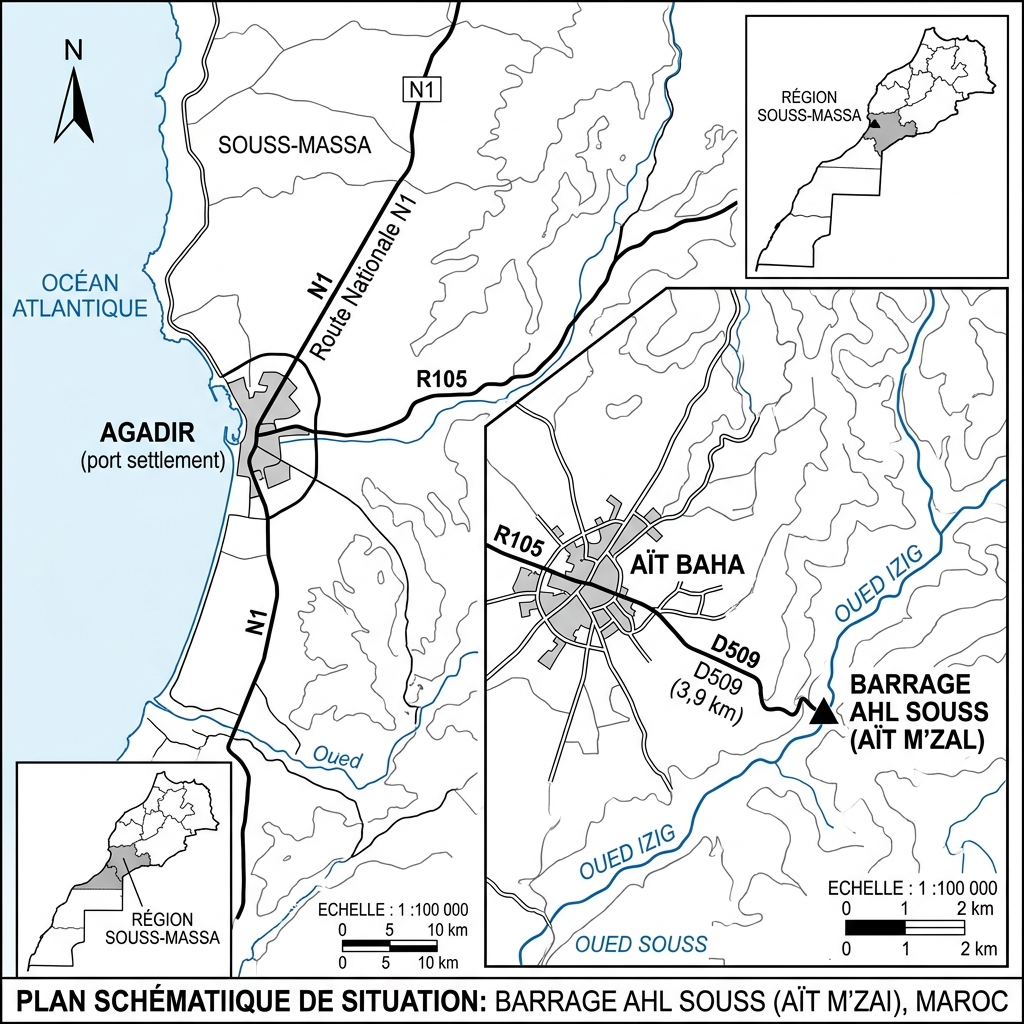
\includegraphics[width=0.55\textwidth]{figures/figure4_location.png}
    \caption{Vue satellitaire du barrage Ahl Souss (A\"it M'zal) sur l'oued Izig, province de Chtouka A\"it Baha. Source : Google Maps (2024).}
    \label{fig:localisation_barrage}
\end{figure}

\section{Caractéristiques hydrologiques}
\label{sec:hydrologie}

Le bassin versant de l'oued Izig présente les caractéristiques physiques suivantes \cite{donnees_hydrologiques, fiche_synoptique} :
\begin{itemize}
    \item Superficie : 187 km²
    \item Altitude moyenne : 1\,287 m
    \item Pluie moyenne annuelle : 269--275 mm
    \item Apport moyen annuel : 5,1 millions de m³ (série de données de 1932 à 2006) \cite{bilans_apports}
    \item Envasement moyen annuel : 100\,000 m³/an
\end{itemize}

Les débits de pointe des crues pour différentes périodes de retour sont \cite{donnees_hydrologiques, fiche_synoptique} :

\begin{table}[H]
    \centering
    \caption{Débits de crues du barrage Ahl Souss}
    \label{tab:debits_crues}
    \begin{tabular}{|c|c|c|}
        \hline
        \textbf{Période de retour (ans)} & \textbf{Débit (m³/s)} & \textbf{Volume (Mm³)} \\
        \hline
        10 & 220 & 2,62 \\
        \hline
        100 & 520 & 6,27 \\
        \hline
        1000 & 820 & 9,85 \\
        \hline
        5000 & 1030 & 12,4 \\
        \hline
    \end{tabular}
\end{table}

L'hydrogramme de crue, supposé triangulaire, présente un temps de base de 7 heures et un temps de montée de 2 heures \cite{donnees_hydrologiques}.

\section{Caractéristiques de la retenue}
\label{sec:retenue}

La retenue du barrage Ahl Souss présente les caractéristiques suivantes \cite{fiche_synoptique, bilans_apports} :
\begin{itemize}
    \item Niveau de retenue normale (RN) : \textbf{600,00 NGM}
    \item Niveau des plus hautes eaux (NPHE) : \textbf{602,86 NGM}
    \item Aire de la retenue au niveau normal : 0,5 km² (50 ha)
    \item Capacité à retenue normale : \textbf{4,76 Mm³}
\end{itemize}

\section{Caractéristiques principales du barrage}
\label{sec:caracteristiques_barrage}

Le barrage Ahl Souss est un ouvrage \textbf{poids en béton compacté au rouleau (BCR)} dont les principales caractéristiques sont \cite{fiche_synoptique, fiche_historique} :
\begin{itemize}
    \item Hauteur maximale sur fondation : 49 m
    \item Hauteur maximale sur terrain naturel : 32,50 m
    \item Longueur en crête : 213,59 m
    \item Largeur en crête : 5 m
    \item Cote de la crête : 604,00 NGM
    \item Fruit du parement amont : \textbf{vertical} (modifié par rapport à l'APD)
    \item Fruit du parement aval : \textbf{0,9 H / 1 V} (modifié)
    \item Volume total de béton : 94\,000 m³ (dont 71\,500 m³ de BCR et 22\,500 m³ de BCV)
\end{itemize}

\section{Description de l'évacuateur de crues}
\label{sec:evacuateur_crues}

L'évacuateur de crues est un ouvrage critique pour la sécurité du barrage, conçu pour transiter les crues exceptionnelles sans endommager l'ouvrage. Ses caractéristiques sont les suivantes \cite{fiche_synoptique, note_calcul_evacuateur} :

\begin{itemize}
    \item \textbf{Type} : Seuil libre en béton de type Creager, implanté dans la partie centrale du barrage.
    \item \textbf{Longueur de déversement} : 70 m.
    \item \textbf{Cote du seuil} : 600,00 NGM (calée au niveau de la retenue normale).
    \item \textbf{Charge maximale sous NPHE} : 2,86 m (calculée après laminage de la crue millénale).
    \item \textbf{Débit évacué sous NPHE} : 730 m³/s.
    \item \textbf{Débit évacué sous NPHEE} : 1\,008 m³/s.
    \item \textbf{Mode de restitution} : Saut de ski.
\end{itemize}

Le profil du seuil, dimensionné pour une charge de 3,20 m, est défini par l'équation \cite{note_calcul_evacuateur} :

\begin{equation}
X^{1,85} = 5{,}376\,Y
\label{eq:profil_creager}
\end{equation}

Le coursier est bordé de murs bajoyers canalisant l'écoulement. La cuillère du saut de ski, calée à la cote \textbf{585,20 NGM}, permet de projeter le jet d'eau loin du pied aval du barrage. Le bec déviateur est tracé selon un arc de cercle de rayon \textbf{3 m} avec un angle de sortie de \textbf{40°} sur l'horizontale \cite{note_calcul_evacuateur}. La distance d'impact du jet est estimée à \textbf{29,5 m} pour la crue de projet.

\section{Description de la vidange de fond}
\label{sec:vidange_fond}

La vidange de fond est un organe essentiel pour la gestion des sédiments et la vidange partielle ou totale de la retenue pour des besoins d'inspection ou de maintenance. Ses caractéristiques sont \cite{fiche_organes_restitution, note_calcul_vidange} :

\begin{itemize}
    \item \textbf{Implantation} : Rive gauche.
    \item \textbf{Type} : Deux conduites en acier indépendantes.
    \item \textbf{Diamètre des conduites} : \textbf{1000 mm} (initialement prévu en 800 mm dans l'APD, modifié en phase d'exécution pour réduire le temps de vidange).
    \item \textbf{Longueur des conduites} : 22,00 m.
    \item \textbf{Cote de calage à l'entrée} : \textbf{585,50 NGM} (ajustée par rapport à la cote 586,00 NGM de l'APD).
    \item \textbf{Volume de retenue correspondant} : 932 788 m³.
    \item \textbf{Capacité sous retenue normale} : \textbf{12 m³/s}.
    \item \textbf{Temps de vidange de la retenue} : \textbf{5 jours}.
    \item \textbf{Équipement hydromécanique} :
    \begin{itemize}
        \item 2 vannes à opercule (papillon) de diamètre 1000 mm par conduite (une vanne de garde et une vanne de réglage), pression nominale 10 Bar.
        \item Une grille métallique de protection de dimensions 1,4 m x 1,4 m.
        \item Commande électrique (moteur 3 kW, 400 V) ou manuelle (volant).
    \end{itemize}
    \item \textbf{Dissipation} : Bassin de dissipation en béton armé de 12 m de longueur, radier à la cote 579,50 NGM, prolongé par un canal en maçonnerie.
\end{itemize}

% SECTION 4.10 : DESCRIPTION DES PRISES D'EAU (AEP ET AGRICOLE)
\section{Description des prises d'eau (AEP et agricole)}
\label{sec:prises_eau}

Le barrage est équipé de plusieurs prises d'eau pour satisfaire les besoins en eau potable et en irrigation \cite{fiche_synoptique, fiche_organes_restitution} :

\begin{itemize}
    \item \textbf{Prises d'eau potable (AEP)} : Trois conduites en acier de diamètre 200 mm, calées à différentes cotes pour permettre un tirage sélectif en fonction de la qualité de l'eau et du niveau de la retenue :
    \begin{itemize}
        \item Cote \textbf{595 NGM}.
        \item Cote \textbf{590 NGM}.
        \item Cote \textbf{586 NGM}.
    \end{itemize}
    Chaque conduite est équipée de vannes de contrôle.
    \item \textbf{Prise agricole} : Une conduite en acier de diamètre 300 mm, calée à la cote \textbf{586,00 NGM}, avec une vanne de contrôle.
\end{itemize}

% SECTION 4.11 : DESCRIPTION DE LA GALERIE D'INJECTION ET DE DRAINAGE
\section{Description de la galerie d'injection et de drainage}
\label{sec:galerie}

Une galerie visiteuse, reliant les deux rives, joue un rôle crucial dans la surveillance et la sécurité de l'ouvrage \cite{fiche_historique, fiche_synoptique} :
\begin{itemize}
    \item \textbf{Fonctions} :
    \begin{itemize}
        \item Permettre l'injection de coulis de ciment pour créer un voile d'étanchéité dans la fondation (injection).
        \item Collecter les eaux de drainage pour mesurer et contrôler les sous-pressions (drainage).
        \item Servir d'accès pour l'inspection et l'auscultation de l'intérieur du barrage.
    \end{itemize}
    \item \textbf{Caractéristiques} : La galerie a été surélevée à la cote \textbf{573,50 NGM} en phase d'exécution (contre 570 NGM à l'APD) pour éviter les risques d'inondation. Sa largeur a été portée à \textbf{3 m} pour faciliter les travaux de forage.
\end{itemize}

% SECTION 4.12 : DESCRIPTION DE LA DÉRIVATION PROVISOIRE
\section{Description de la dérivation provisoire}
\label{sec:derivation_provisoire}

Pendant la construction, il a fallu dévier l'oued pour travailler à sec \cite{fiche_historique, fiche_synoptique} :
\begin{itemize}
    \item \textbf{Type} : Deux pertuis bétonnés disposés en rive gauche, traversant provisoirement le corps du barrage.
    \item \textbf{Dimensions des pertuis} : 2 x 4,50 m de large x 5,00 m de haut.
    \item \textbf{Crue de chantier} : Dimensionnée pour la crue vingtenale (Q20 = 310 m³/s).
\end{itemize}

% SECTION 4.13 : ASPECTS PARTICULIERS ET ADAPTATIONS EN COURS DE CHANTIER
\section{Aspects particuliers et adaptations en cours de chantier}
\label{sec:adaptations_chantier}

Plusieurs adaptations ont été apportées au projet initial (APD) durant la phase d'exécution pour s'adapter aux conditions réelles du site ou pour optimiser l'ouvrage \cite{fiche_historique, note_geologique_2003} :

\begin{itemize}
    \item \textbf{Décalage de l'axe du barrage} : L'axe définitif a été décalé d'une trentaine de mètres en aval suite aux prospections géologiques qui ont révélé du rocher altéré sur la rive gauche.
    \item \textbf{Modification du profil du barrage} : Le profil est passé d'un parement amont penté (0,2H/1V) à un parement amont \textbf{vertical}, et le parement aval de 0,8H/1V à \textbf{0,9H/1V}. La largeur en crête est passée de 3 m à \textbf{5 m}, et sa cote de 603,50 à \textbf{604,00 NGM}.
    \item \textbf{Approfondissement des fouilles} : La découverte d'une zone de rocher très altéré en fond de vallée (épaisseur de 7 à 8 m) a nécessité un approfondissement des fouilles de 7 à 9 m, avec des cotes de fondation finales à 555 NGM (amont) et 556 NGM (aval).
    \item \textbf{Élargissement du diamètre des conduites de vidange} : Le diamètre est passé de 800 mm à \textbf{1000 mm}, réduisant le temps de vidange de la retenue d'environ 64 \%.
    \item \textbf{Surélévation de la galerie d'injection} : La galerie a été surélevée de la cote 570 NGM à \textbf{573,50 NGM} pour éviter les risques d'inondation.
    \item \textbf{Substitution du BCR par du BCV pour le couronnement} : Le BCR prévu pour le couronnement (cotes 598,45 à 604,00 NGM) a été remplacé par du BCV en raison de l'espace de travail trop restreint pour les engins de compactage.
\end{itemize}

% SECTION 4.14 : CONCLUSION
\section{Conclusion}
\label{sec:conclusion_chap4}

Le barrage Ahl Souss constitue un ouvrage hydraulique complexe, dont la conception a intégré des innovations technologiques comme le béton compacté au rouleau, et a su s'adapter aux contraintes géologiques et opérationnelles rencontrées en cours de chantier. La description détaillée de ses caractéristiques et de ses organes annexes, notamment l'évacuateur de crues et la vidange de fond, pose les bases nécessaires à la modélisation numérique qui fera l'objet de la suite de ce rapport.


% --- DEUXIÈME PARTIE : REVUE DES LOGICIELS CFD ---
\part{DEUXIÈME PARTIE : REVUE DES LOGICIELS CFD}

% ============================================================
%  CHAPITRE 5 : Benchmark des logiciels de modélisation 3D
% ============================================================
\chapter{Benchmark des logiciels de modélisation 3D}
\label{chap:benchmark_logiciels}

% SECTION 5.1 : INTRODUCTION
\section{Introduction}
\label{sec:introduction_benchmark}

La modélisation 3D des écoulements dans les ouvrages hydrauliques est devenue un outil essentiel pour l'analyse et l'optimisation des performances. De nombreux logiciels CFD sont disponibles, chacun présentant des caractéristiques spécifiques en termes de méthodes numériques, de modèles physiques, de type de maillage et d'accessibilité (open source ou commercial). Ce chapitre propose une analyse comparative des principales solutions logicielles adaptées à la modélisation des écoulements à surface libre, afin de justifier le choix d'OpenFOAM pour la présente étude.

% SECTION 5.2 : PRÉSENTATION DES LOGICIELS
\section{Présentation des logiciels}
\label{sec:presentation_logiciels}

\subsection{TELEMAC-3D}
\label{subsec:telemac}

TELEMAC-3D est un code de calcul open source développé par le Laboratoire National d'Hydraulique et Environnement (LNHE) d'EDF R\&D. Il résout les équations de Navier-Stokes pour les écoulements à surface libre, en utilisant la méthode des \textbf{éléments finis}. Il est particulièrement adapté à l'hydrodynamique côtière, estuarienne et fluviale, ainsi qu'au transport de sédiments et à la qualité de l'eau. Sa flexibilité et sa gratuité en font un outil académique et professionnel de premier plan, mais sa prise en main peut être complexe \cite{galland1991telemac, hervouet2007hydrodynamics}.

\subsection{Flow-3D}
\label{subsec:flow3d}

Flow-3D est un logiciel commercial CFD développé par Flow Science. Il est réputé pour sa capacité à modéliser avec précision les écoulements à surface libre grâce à la méthode \textbf{VOF (Volume of Fluid)}, dont il est l'un des pionniers \cite{hirt1981volume}. Il utilise un maillage structuré cartésien, ce qui simplifie la génération du maillage. Sa méthode \textbf{FAVOR (Fractional Area/Volume Obstacle Representation)} permet de représenter des géométries complexes sur un maillage simple \cite{flow2016user}. Il est très utilisé en hydraulique (déversoirs, ressauts, dissipateurs d'énergie) mais est payant.

\subsection{ANSYS Fluent}
\label{subsec:ansys_fluent}

Ansys Fluent est l'un des logiciels CFD commerciaux les plus complets et les plus utilisés dans le monde, toutes industries confondues (aéronautique, automobile, énergie, hydraulique). Il utilise la méthode des \textbf{volumes finis} sur des maillages non structurés (polyédriques, tétraédriques, hexaédriques). Il dispose d'une très large bibliothèque de modèles physiques (turbulence, multiphasique, combustion, etc.) et d'une interface utilisateur graphique très avancée \cite{ansys2020fluent, matsson2022introduction}. Sa puissance a un coût élevé en termes de licence.

\subsection{XFlow}
\label{subsec:xflow}

XFlow est un logiciel CFD commercial de nouvelle génération développé par Dassault Systèmes. Il se distingue par son approche innovante : il n'utilise pas de maillage traditionnel mais une méthode particulaire basée sur la \textbf{méthode de Lattice Boltzmann} \cite{chen1998lattice, kruger2017lattice}. Cette approche sans maillage est très efficace pour traiter des géométries complexes en mouvement et des écoulements instationnaires. Il est plus récent et son application en hydraulique "classique" est en développement.

\subsection{STAR-CCM+}
\label{subsec:starccm}

STAR-CCM+ est un logiciel commercial CFD développé par Siemens. Il est reconnu pour son interface unifiée et son workflow intégré, de la préparation de la géométrie à l'analyse des résultats. Il utilise également la méthode des volumes finis et a popularisé l'utilisation de maillages polyédriques, qui offrent un bon compromis entre précision et nombre de cellules \cite{cd2019star, peric2005advantage}. Il est très présent dans les secteurs automobile et aéronautique.

\subsection{OpenFOAM}
\label{subsec:openfoam}

OpenFOAM (Open Field Operation and Manipulation) est la principale solution \textbf{open source} en CFD. Développé par OpenCFD Ltd, il s'agit d'une bibliothèque de solveurs et d'outils écrits en C++, permettant de résoudre une vaste gamme de problèmes en mécanique des fluides (et des solides) \cite{weller1998tensorial, jasak2009openfoam}. Il utilise la méthode des volumes finis sur des maillages non structurés. Son principal avantage est sa gratuité, sa transparence (code source accessible) et sa flexibilité : l'utilisateur peut modifier les solveurs existants ou en créer de nouveaux. L'inconvénient est l'absence d'interface graphique native et une courbe d'apprentissage plus raide.

\subsection{SimScale}
\label{subsec:simscale}

SimScale est une plateforme de simulation \textbf{cloud} (SaaS - Software as a Service). Elle propose un accès à des solveurs de CFD (basés sur OpenFOAM) et d'analyse par éléments finis via un navigateur web \cite{simscale2021documentation, bletzinger2017cloud}. Elle fonctionne sur un modèle freemium (compte gratuit avec des limitations) ou par abonnement. Son avantage est l'accessibilité sans nécessiter de matériel puissant, mais la confidentialité des données peut être une préoccupation.

\subsection{Autres logiciels}
\label{subsec:autres_logiciels}

D'autres logiciels complètent le paysage des solutions disponibles :
\begin{itemize}
    \item \textbf{Autodesk CFD} : Solution commerciale d'Autodesk, basée sur la méthode des éléments finis, intégrée dans l'écosystème de conception.
    \item \textbf{ANSYS CFX} : Autre solveur CFD majeur d'Ansys, réputé pour sa robustesse et sa précision, notamment pour les turbomachines.
    \item \textbf{MIKE 3 Wave FM} : Logiciel commercial de DHI, spécialisé dans l'hydrodynamique côtière et maritime (vagues, courants) \cite{dhi2020mike}.
    \item \textbf{COMSOL Multiphysics} : Plateforme commerciale permettant de coupler la CFD avec d'autres physiques (électromagnétisme, thermique, mécanique des structures) \cite{comsol2021reference}.
\end{itemize}

% SECTION 5.3 : COMPARAISON ENTRE LES LOGICIELS
\section{Comparaison entre les logiciels}
\label{sec:comparaison_logiciels}

Le tableau suivant regroupe les principales caractéristiques des logiciels présentés :

\begin{table}[H]
    \centering
    \caption{Comparaison des principaux logiciels de CFD}
    \label{tab:comparaison_logiciels_cfd}
    \resizebox{\textwidth}{!}{%
    \begin{tabular}{|l|c|c|c|c|c|}
        \hline
        \textbf{Logiciel} & \textbf{Interface graphique} & \textbf{Méthode} & \textbf{Maillage 3D} & \textbf{Open source} & \textbf{Coût} \\
        \hline
        TELEMAC-3D & Oui & Éléments finis & Non structuré & \textbf{Oui} & \textbf{Gratuit} \\
        \hline
        Flow-3D & Oui & Volumes finis & Cartésien structuré & Non & Payant \\
        \hline
        ANSYS Fluent & Oui & Volumes finis & Non structuré (polyédrique) & Non & Payant \\
        \hline
        XFlow & Oui & Lattice Boltzmann & Sans maillage & Non & Payant \\
        \hline
        STAR-CCM+ & Oui & Volumes finis & Non structuré (polyédrique) & Non & Payant \\
        \hline
        \textbf{OpenFOAM} & \textbf{Non} (via ParaView) & Volumes finis & Non structuré & \textbf{Oui} & \textbf{Gratuit} \\
        \hline
        SimScale & Oui (cloud) & Volumes finis / EF & Automatique (cloud) & Basé sur OpenFOAM & Freemium \\
        \hline
        ANSYS CFX & Oui & Volumes finis (couplé) & Non structuré & Non & Payant \\
        \hline
    \end{tabular}}
\end{table}

% SECTION 5.4 : LE LOGICIEL SKETCHUP
\section{Le logiciel SketchUp}
\label{sec:sketchup}

Bien que n'étant pas un logiciel de CFD, SketchUp joue un rôle important dans la chaîne de modélisation pour la création de la géométrie. Dans notre démarche, les profils types 2D des ouvrages ont d'abord été réalisés sous \textbf{AutoCAD}, puis importés dans SketchUp afin de servir de base à la modélisation 3D.

\subsection{Présentation du logiciel}
\label{subsec:presentation_sketchup}

SketchUp est un logiciel de modélisation 3D développé par Trimble Inc., reconnu pour la simplicité et l'intuitivité de son interface \cite{trimble2023sketchup, brightman2018sketchup}. Contrairement aux logiciels BIM paramétriques (comme Revit), SketchUp repose sur une modélisation directe à base de faces et d'arêtes, manipulées à l'aide d'outils simples tels que ``Pousser/Tirer'' (Push/Pull), ``Suivez-moi'' ou encore les outils de mise à l'échelle et de rotation. Les éléments peuvent être organisés en \textbf{groupes} et \textbf{composants}, ce qui permet de structurer le modèle et de réutiliser des éléments identiques.

\subsection{Intérêt pour la modélisation des ouvrages hydrauliques}
\label{subsec:interet_sketchup}

Pour la modélisation des ouvrages hydrauliques comme le barrage Ahl Souss, SketchUp présente plusieurs avantages significatifs :

\begin{itemize}
    \item \textbf{Rapidité et simplicité de modélisation} : les outils de modélisation directe (Pousser/Tirer, Suivez-moi) permettent de générer rapidement des géométries complexes (corps du barrage, seuil Creager, coursier, conduites de vidange, murs bajoyers, prises d'eau) à partir de profils 2D \cite{brightman2018sketchup}.
    \item \textbf{Modélisation du terrain naturel} : l'outil \textit{Sandbox} de SketchUp permet de générer une surface topographique (TIN) directement à partir des courbes de niveau, facilitant l'intégration du terrain naturel dans le modèle global.
    \item \textbf{Organisation en groupes et composants} : chaque élément de l'ouvrage peut être isolé dans un groupe ou un composant dédié, ce qui simplifie les modifications et la gestion des différentes parties du modèle.
    \item \textbf{Exportation vers les formats CAO standards} : grâce à l'extension \textbf{SketchUp STL}, les modèles 3D peuvent être exportés au format \textbf{STL (Standard Tessellation Language)} \cite{lhuillier2014sketchupstl}. Ce format, qui décrit une géométrie par un maillage de triangles, est compatible avec la plupart des logiciels de CFD, dont OpenFOAM.
    \item \textbf{Accessibilité} : SketchUp est disponible en version gratuite (SketchUp Free, en ligne) et en version professionnelle à coût modéré, ce qui en fait un outil accessible pour des projets académiques.
\end{itemize}

\subsection{Démarche de modélisation}
\label{subsec:demarche_sketchup}

Le processus de modélisation pour notre étude comprend les étapes suivantes :
\begin{enumerate}
    \item Réalisation du profil type 2D du barrage (cote de fondation, fruit des parements, largeur en crête) et de l'évacuateur de crues sous \textbf{AutoCAD}.
    \item Importation du profil 2D AutoCAD dans un projet SketchUp avec les unités appropriées (mètres).
    \item Modélisation du terrain naturel à l'aide de l'outil \textit{Sandbox} à partir des données topographiques (courbes de niveau).
    \item Création du corps du barrage par extrusion (Pousser/Tirer) du profil type importé depuis AutoCAD.
    \item Modélisation de l'évacuateur de crues (seuil Creager, coursier, cuillère) à l'aide des outils de courbes et de l'outil \textit{Suivez-moi}.
    \item Modélisation de la vidange de fond (conduites, chambre des vannes, bassin de dissipation).
    \item Modélisation des prises d'eau et de la galerie.
    \item Exportation au format STL via l'extension SketchUp STL pour une utilisation dans OpenFOAM \cite{lhuillier2014sketchupstl}.
\end{enumerate}

% SECTION 5.5 : CONCLUSION
\section{Conclusion}
\label{sec:conclusion_benchmark}

Le choix d'OpenFOAM pour cette étude se justifie par plusieurs avantages : sa gratuité, l'accès au code source permettant une transparence totale et une flexibilité maximale, sa capacité de calcul parallèle (HPC) pour traiter des géométries complexes, et sa large communauté d'utilisateurs qui garantit un support et un partage de connaissances. Sa structure modulaire permet d'adapter précisément les modèles physiques aux spécificités des ouvrages du barrage Ahl Souss. Associé à SketchUp pour la modélisation géométrique 3D, cet ensemble d'outils constitue une chaîne de simulation complète, performante et économiquement accessible.



% --- TROISIÈME PARTIE : SIMULATION HYDRAULIQUE ET DIMENSIONNEMENT ---
\part{TROISIÈME PARTIE : SIMULATION HYDRAULIQUE ET DIMENSIONNEMENT DE L'ÉVACUATEUR DE CRUES}

% ============================================================
%  CHAPITRE 6 : Structure d'un code CFD et d'un cas OpenFOAM
% ============================================================
\chapter{Structure d'un code CFD et d'un cas OpenFOAM}
\label{chap:structure_cfd_openfoam}

% SECTION : INTRODUCTION
\section{Introduction}
\label{sec:introduction_structure_cfd_openfoam}

La mécanique des fluides numérique (CFD) permet de simuler des écoulements complexes en résolvant numériquement les équations de conservation. Pour cela, un code CFD suit une structure bien définie, articulée autour de trois étapes principales : le pré-traitement, la résolution et le post-traitement \cite{wendt2009computational}. Chacune de ces phases est indispensable pour garantir la fiabilité des résultats, depuis la préparation du modèle jusqu'à l'analyse des données simulées.

Ce chapitre présente dans un premier temps cette structure générale, puis détaille la manière dont OpenFOAM l'implémente concrètement : son organisation de fichiers, ses solveurs, ses algorithmes de résolution numérique, ainsi que ses outils de visualisation et de post-traitement.

% SECTION : STRUCTURE GÉNÉRALE D'UN CODE CFD
\section{Structure générale d'un code CFD}
\label{sec:structure_generale_code_cfd}

\subsection{Pré-traitement (Pre-processing)}
\label{subsec:preprocessing}

Cette étape consiste à préparer les données nécessaires à la simulation. Cela inclut la définition du domaine géométrique sous forme maillée, le choix des phénomènes physiques à modéliser (comme la turbulence, les écoulements multiphasiques ou la cavitation), ainsi que la spécification des propriétés physiques du fluide et des conditions aux limites adaptées au cas étudié \cite{thompson1999handbook}. Les grandeurs à calculer, telles que la vitesse, la pression et la température, sont associées aux nœuds de chaque cellule du maillage.

La qualité du maillage est cruciale pour la précision des résultats. Les paramètres clés incluent la résolution spatiale, la qualité des cellules (skewness, orthogonalité) et le raffinement local dans les zones à forts gradients \cite{knupp1993fundamentals}.

\subsection{Résolution (Processing)}
\label{subsec:processing}

Le rôle du solveur est d'appliquer les algorithmes permettant \cite{patankar1980numerical} :
\begin{itemize}
    \item D'intégrer les équations de conservation sur chaque volume de contrôle.
    \item De transformer ces équations intégrales en un système algébrique.
    \item D'en estimer la solution à l'aide de méthodes itératives.
\end{itemize}

La majorité des logiciels de CFD, dont OpenFOAM, utilise la méthode des \textbf{volumes finis}, qui repose sur l'application directe des bilans sur chaque volume de contrôle. Cette approche est largement adoptée en raison de sa rigueur et de son efficacité, ce qui explique son succès auprès des éditeurs de logiciels de simulation numérique \cite{versteeg2007introduction}.

\subsection{Post-traitement (Post-processing)}
\label{subsec:postprocessing}

Le post-traitement vise avant tout à évaluer la qualité de la solution obtenue. Il s'agit notamment de vérifier si cette solution est indépendante de la taille du maillage, du critère de convergence et des schémas numériques utilisés \cite{roache1998verification}. Il est également essentiel de s'assurer que le modèle de turbulence ainsi que les conditions aux limites ont été choisis de manière pertinente, et d'analyser dans quelle mesure les résultats dépendent de ces choix.

En général, le solveur fournit une grande quantité de données brutes, telles que les champs de vitesse (u, v, w), de pression (p), etc., pour chaque point du maillage. Ces données doivent être converties en représentations visuelles afin de faciliter leur analyse et leur compréhension \cite{schroeder2006visualization}.

Les principaux résultats généralement présentés lors du post-traitement sont les suivants \cite{hansen2011visualization} :
\begin{itemize}
    \item La représentation de la géométrie du domaine et des détails du maillage.
    \item L'évolution de la convergence au cours des itérations (graphique des résidus).
    \item Les champs et profils de vitesse (contours, vecteurs, lignes de courant).
    \item Les tracés des distributions de pression.
    \item Les animations et visualisations dynamiques des écoulements simulés.
\end{itemize}

% SECTION : STRUCTURE GÉNÉRALE D'UN CAS OPENFOAM
\section{Structure générale d'un cas OpenFOAM}
\label{sec:structure_openfoam}

OpenFOAM adopte une structure de fichiers standardisée, organisée de manière logique pour séparer les différents aspects du cas \cite{openfoam2022guide}. Cette hiérarchie de fichiers facilite la lisibilité, la modification et l'automatisation des cas de calcul. Un cas OpenFOAM comprend trois répertoires principaux : \textbf{``0''}, \textbf{``constant''} et \textbf{``system''} \cite{greenshields2020openfoam}.

% SECTION : LES SOLVEURS DISPONIBLES DANS OPENFOAM
\section{Les solveurs disponibles dans OpenFOAM}
\label{sec:solveurs_openfoam}

OpenFOAM propose une vaste bibliothèque de solveurs classés par type d'écoulement \cite{jasak1996error} :

\begin{table}[H]
    \centering
    \caption{Classification des solveurs dans OpenFOAM}
    \label{tab:solveurs_openfoam}
    \resizebox{\textwidth}{!}{%
    \begin{tabular}{|l|l|l|}
        \hline
        \textbf{Type d'écoulement} & \textbf{Solveurs} & \textbf{Description} \\
        \hline
        Basique & laplacianFoam & Diffusion thermique dans un solide \\
        \hline
        & potentialFoam & Écoulement potentiel pour initialisation \\
        \hline
        Incompressible & icoFoam & Transitoire, laminaire, isotherme \\
        \hline
        & simpleFoam & Permanent, turbulent (algorithme SIMPLE) \\
        \hline
        & pisoFoam & Transitoire, turbulent (algorithme PISO) \\
        \hline
        & pimpleFoam & Transitoire, grand pas de temps (algorithme PIMPLE) \\
        \hline
        Compressible & rhoCentralFoam & Basé sur Kurganov-Tadmor, ondes de choc \\
        \hline
        & rhoPimpleFoam & Transitoire, laminaire ou turbulent \\
        \hline
        & rhoSimpleFoam & Permanent, RANS \\
        \hline
        Multiphase & \textbf{interFoam} & \textbf{2 fluides incompressibles, méthode VOF} \\
        \hline
        & cavitatingFoam & Transitoire, cavitation \\
        \hline
        & multiphaseInterFoam & n fluides incompressibles \\
        \hline
    \end{tabular}}
\end{table}

Pour notre étude, le solveur \textbf{interFoam} est choisi car il est spécifiquement conçu pour les écoulements diphasiques incompressibles avec suivi d'interface par la méthode VOF \cite{rusche2002computational}, ce qui est parfait pour modéliser la surface libre de l'eau dans l'évacuateur de crues.

% SECTION : LES ALGORITHMES DE RÉSOLUTION NUMÉRIQUE
\section{Les algorithmes de résolution numérique}
\label{sec:algorithmes_resolution}

Les équations de Navier-Stokes établissent une relation linéaire entre la pression et la vitesse. Cependant, la pression ne dispose pas d'une équation propre permettant sa résolution directe. Plusieurs algorithmes sont disponibles pour assurer le couplage pression-vitesse \cite{patankar1972calculation} :

\subsection{L'algorithme SIMPLE}
\label{subsec:simple}

L'algorithme SIMPLE (Semi-Implicit Method for Pressure-Linked Equations) est une méthode itérative pour les écoulements \textbf{stationnaires} \cite{caretto1973two}. Il procède par une séquence d'étapes à chaque itération : estimation d'un champ de vitesse à partir d'un champ de pression estimé, puis résolution d'une équation de correction de pression pour satisfaire la continuité, et enfin mise à jour de la pression et de la vitesse. Le processus est répété jusqu'à convergence.

\subsection{L'algorithme PISO}
\label{subsec:piso}

L'algorithme PISO (Pressure Implicit with Splitting of Operator) est spécifiquement adapté aux écoulements \textbf{transitoires} \cite{issa1986solution}. À chaque pas de temps, il effectue une étape de prédiction de la vitesse, suivie de plusieurs étapes de correction de pression (généralement deux) pour satisfaire la continuité de manière plus précise que SIMPLE.

\subsection{L'algorithme PIMPLE}
\label{subsec:pimple}

L'algorithme PIMPLE combine les deux approches, PISO et SIMPLE. Il s'agit d'une implémentation de l'algorithme PISO avec la possibilité d'utiliser un facteur de sous-relaxation (comme dans SIMPLE) et d'effectuer des itérations externes à l'intérieur d'un même pas de temps. Cela permet d'utiliser des pas de temps plus grands que ceux imposés par la condition de Courant, améliorant ainsi l'efficacité pour les simulations transitoires avec des maillages complexes \cite{holzmann2017mathematics}.

% SECTION : STABILITÉ ET CONVERGENCE DES CALCULS
\section{Stabilité et convergence des calculs}
\label{sec:stabilite_convergence}

\subsection{Définitions}
\label{subsec:definitions}

La \textbf{stabilité} en simulation CFD désigne la capacité d'une méthode numérique à générer des résultats bornés et réalistes, sans amplification incontrôlée des erreurs numériques \cite{courant1928uber}. La \textbf{convergence} correspond à la capacité d'une méthode numérique à fournir une solution qui se rapproche de la solution exacte des équations discrétisées à mesure que le calcul itératif progresse (ou que le maillage est raffiné) \cite{ferziger2002computational}.

\subsection{Paramètres influençant la convergence}
\label{subsec:parametres_convergence}

Les principaux paramètres influençant la convergence, la stabilité et la durée d'une simulation CFD sont \cite{hirsch2007numerical} :
\begin{itemize}
    \item La discrétisation spatiale (taille et qualité du maillage).
    \item La discrétisation temporelle (pas de temps $\Delta t$).
    \item Le choix du modèle de turbulence et de ses paramètres.
    \item La méthode de résolution et le type de solveur (SIMPLE, PISO, etc.).
    \item Les conditions aux limites et initiales.
    \item Les propriétés physiques du fluide ($\rho$, $\mu$).
\end{itemize}

\subsection{Critères de stabilité}
\label{subsec:criteres_stabilite}

Pour garantir la stabilité d'un calcul CFD explicite, il est essentiel de respecter le critère de Courant-Friedrichs-Lewy (CFL) \cite{leveque2007finite}. Le nombre de Courant est défini par :

\begin{equation}
Co = \frac{|U| \cdot \Delta t}{\Delta x}
\label{eq:courant}
\end{equation}

La condition de stabilité s'exprime par \( Co \leq 1 \), garantissant que l'information (une particule fluide) ne parcourt pas plus d'une cellule à chaque pas de temps \cite{trefethen1996finite}. Pour les schémas implicites, la condition est moins restrictive, mais un Co trop grand peut encore dégrader la précision.

% SECTION : LE SYSTÈME DE FICHIERS D'OPENFOAM
\section{Le système de fichiers d'OpenFOAM}
\label{sec:fichiers_openfoam}

\subsection{Le dossier ``0''}
\label{subsec:dossier_0}

Le dossier ``0'' contient les dictionnaires définissant les \textbf{conditions initiales et aux limites} pour chaque champ (pression \texttt{p}, vitesse \texttt{U}, fraction volumique \texttt{alpha.water}, paramètres de turbulence \texttt{k}, \texttt{omega}, \texttt{nut}) à l'instant initial ($t=0$) \cite{moukalled2016finite}.

Les principales conditions aux limites disponibles dans OpenFOAM sont \cite{openfoam2022boundary} :

\begin{table}[H]
    \centering
    \caption{Conditions aux limites courantes dans OpenFOAM}
    \label{tab:boundary_conditions}
    \resizebox{\textwidth}{!}{%
    \begin{tabular}{|l|l|l|}
        \hline
        \textbf{Type} & \textbf{Description} & \textbf{Application typique} \\
        \hline
        \texttt{fixedValue} & Valeur fixée par l'utilisateur & Vitesse d'entrée (\texttt{U}) \\
        \hline
        \texttt{zeroGradient} & Gradient normal nul & Sortie libre (\texttt{p}) \\
        \hline
        \texttt{fixedGradient} & Gradient normal fixé & Flux de chaleur imposé \\
        \hline
        \texttt{inletOutlet} & fixedValue en entrée, zeroGradient en sortie & Sortie avec risque de reflux (\texttt{U}) \\
        \hline
        \texttt{totalPressure} & Pression totale constante & Entrée avec pression imposée \\
        \hline
        \texttt{pressureInletOutletVelocity} & U évalué à partir de p & Surface libre, sortie \\
        \hline
        \textbf{\texttt{noSlip}} & \textbf{Vitesse nulle à la paroi} & \textbf{Parois solides} \\
        \hline
        \texttt{slip} & Glissement parfait & Symétrie \\
        \hline
        \texttt{kqRWallFunction} & Condition de paroi pour k, q, R & Parois turbulentes \\
        \hline
        \texttt{omegaWallFunction} & Condition de paroi pour $\omega$ & Parois turbulentes \\
        \hline
    \end{tabular}}
\end{table}

\subsection{Le dossier ``constant''}
\label{subsec:dossier_constant}

Le dossier ``constant'' regroupe les paramètres indépendants du temps \cite{greenshields2020openfoam} :
\begin{itemize}
    \item \textbf{Propriétés physiques} : \texttt{transportProperties} (viscosité, masse volumique, tension superficielle pour les écoulements multiphasiques).
    \item \textbf{Modélisation de la turbulence} : \texttt{turbulenceProperties} (choix du modèle RANS/LES, type de modèle \texttt{kOmegaSST}, etc.).
    \item \textbf{Maillage} : sous-dossier \texttt{polyMesh} contenant la description complète du maillage (points, faces, cellules, frontières).
    \item \textbf{Géométries STL} : sous-dossier \texttt{triSurface} pour les fichiers de surface (utile pour \texttt{snappyHexMesh}).
\end{itemize}

\subsection{Le dossier ``system''}
\label{subsec:dossier_system}

Le dossier ``system'' contient les fichiers de contrôle de la simulation \cite{jasak2009openfoam} :
\begin{itemize}
    \item \textbf{\texttt{controlDict}} : paramètres temporels (startTime, endTime, deltaT, writeInterval).
    \item \textbf{\texttt{fvSchemes}} : schémas de discrétisation pour les dérivées spatiales (\texttt{gradSchemes}, \texttt{divSchemes}, \texttt{laplacianSchemes}) et temporelles (\texttt{ddtSchemes}).
    \item \textbf{\texttt{fvSolution}} : solveurs linéaires, critères de convergence et algorithmes de couplage (SIMPLE, PISO, PIMPLE).
    \item \textbf{\texttt{blockMeshDict}} : génération du maillage structuré de base.
    \item \textbf{\texttt{snappyHexMeshDict}} : configuration du raffinement autour des géométries complexes (STL) et ajout de couches limites.
    \item \textbf{\texttt{decomposeParDict}} : configuration du calcul parallèle (décomposition du domaine).
\end{itemize}

% SECTION : OUTIL DE VISUALISATION ET DE POST-TRAITEMENT (PARAVIEW)
\section{Outil de visualisation et de post-traitement (ParaView)}
\label{sec:paraview}

\textbf{ParaView} constitue l'outil principal de visualisation et de post-traitement des résultats dans OpenFOAM \cite{ahrens2005paraview}. C'est un logiciel open source puissant qui s'appuie sur un module de lecture intégré à OpenFOAM (\texttt{foamToVTK} ou \texttt{paraFoam}). Pour le lancer, il suffit d'exécuter la commande \texttt{paraFoam} depuis le répertoire du cas concerné.

Cet outil très puissant permet d'afficher divers types de données tels que des champs scalaires (pression, température), des vecteurs (vitesse), des lignes de courant ou encore des surfaces de niveau (pour la surface libre avec \texttt{alpha.water}) \cite{ayachit2015paraview}. Il facilite la création d'animations pour visualiser l'évolution des phénomènes simulés.

% SECTION : MODÉLISATION DE LA SURFACE LIBRE - MÉTHODE VOF
\section{Modélisation de la surface libre - Méthode VOF}
\label{sec:vof}

La méthode \textbf{VOF (Volume of Fluid)} est la plus répandue pour suivre l'interface entre deux fluides non miscibles (par exemple, l'eau et l'air) \cite{hirt1981volume}. Elle utilise un champ scalaire \(\alpha\) (fraction volumique) défini par :

\begin{equation}
\alpha = \frac{V_{eau}}{V_{cellule}}
\label{eq:vof_alpha}
\end{equation}

\(\alpha\) varie entre 0 (cellule pleine d'air) et 1 (cellule pleine d'eau). L'interface est située dans les cellules où \(0 < \alpha < 1\). Le transport de \(\alpha\) est régi par l'équation d'advection \cite{rider1998reconstructing} :

\begin{equation}
\frac{\partial \alpha}{\partial t} + \nabla \cdot (\alpha \vec{U}) = 0
\label{eq:vof_transport}
\end{equation}

Les propriétés du fluide (masse volumique \(\rho\) et viscosité \(\mu\)) sont ensuite calculées par une moyenne pondérée \cite{scardovelli1999direct} :

\begin{align}
\rho &= \alpha \rho_{eau} + (1-\alpha)\rho_{air} \label{eq:vof_rho} \\
\mu &= \alpha \mu_{eau} + (1-\alpha)\mu_{air} \label{eq:vof_mu}
\end{align}

Le solveur \texttt{interFoam} d'OpenFOAM implémente cette méthode avec des techniques avancées de compression de l'interface pour maintenir sa netteté.

% SECTION : CONCLUSION
\section{Conclusion}
\label{sec:conclusion_structure_cfd_openfoam}

La simulation CFD repose sur trois étapes essentielles : le pré-traitement, la résolution et le post-traitement. Chacune joue un rôle clé dans la qualité et l'interprétation des résultats. Une bonne préparation du modèle, un solveur fiable et une analyse rigoureuse garantissent des simulations précises et exploitables.

Ce chapitre a également permis d'explorer la manière dont OpenFOAM met en œuvre cette structure générale, en abordant les différents solveurs disponibles, les algorithmes de résolution numérique (SIMPLE, PISO, PIMPLE), ainsi que les notions essentielles de stabilité et de convergence des calculs. L'organisation des dossiers du logiciel a également été examinée, mettant en lumière la clarté et la logique qui facilitent la gestion des simulations. La méthode VOF, implémentée dans le solveur \texttt{interFoam}, est l'outil idéal pour notre modélisation de l'écoulement dans l'évacuateur de crues.

Il ressort de cette étude que la richesse des solveurs et des algorithmes proposés par OpenFOAM permet de traiter une large gamme de problématiques en mécanique des fluides numérique. Le respect des critères de stabilité et de convergence reste essentiel pour garantir la qualité et la fiabilité des résultats obtenus.

% ============================================================
%  CHAPITRE 7 : Dimensionnement théorique de l'évacuateur de crues
% ============================================================
\chapter{Dimensionnement théorique de l'évacuateur de crues}
\label{chap:dimensionnement_theorique}

% SECTION : INTRODUCTION
\section{Introduction}
\label{sec:intro_dimensionnement}

Avant d'entreprendre la modélisation numérique de l'évacuateur de crues du barrage Ahl Souss sous OpenFOAM, il est indispensable de disposer d'un cadre de référence théorique permettant à la fois de vérifier la cohérence du dimensionnement existant et de constituer une base de comparaison pour les résultats issus de la simulation 3D. Cette démarche correspond à la pratique courante de l'ingénierie hydraulique, où les méthodes analytiques classiques, les feuilles de calcul et les modèles 1D (HEC-RAS) sont systématiquement mobilisés en amont, voire en parallèle, des outils de simulation tridimensionnelle.

Ce chapitre reprend les données géométriques et hydrauliques du barrage Ahl Souss présentées au chapitre \ref{chap:barrage} et les exploite pour mener, étape par étape, le dimensionnement hydraulique complet de l'évacuateur de crues : vérification du profil du seuil déversant (section \ref{sec:profil_seuil}), établissement de la loi débit-charge (section \ref{sec:loi_debit_charge}), calcul de la courbe de remous le long du coursier (section \ref{sec:courbe_remous}), détermination de la hauteur des murs bajoyers à l'aide du logiciel HEC-RAS (section \ref{sec:murs_bajoyers}), vérification de la géométrie de la cuillère du saut de ski (section \ref{sec:geometrie_cuillere}), calcul de la distance d'impact du jet (section \ref{sec:distance_impact_jet}) et évaluation de l'affouillement à l'aval de l'ouvrage (section \ref{sec:affouillement}). L'ensemble de ces résultats est synthétisé en fin de chapitre (section \ref{sec:synthese_resultats_theoriques}) sous la forme d'un tableau récapitulatif qui servira de référence pour l'analyse comparative menée au chapitre \ref{chap:resultats_simulation}.

% SECTION : DONNÉES DE BASE ET HYPOTHÈSES DE CALCUL
\section{Données de base et hypothèses de calcul}
\label{sec:donnees_base_hypotheses}

Les calculs développés dans ce chapitre s'appuient sur les caractéristiques géométriques et hydrologiques du barrage Ahl Souss présentées au chapitre \ref{chap:barrage} : longueur déversante du seuil, cote de calage, charge de dimensionnement du profil, niveaux caractéristiques de la retenue (RN, NPHE), ainsi que sur les débits de pointe des crues de référence rappelés au tableau \ref{tab:debits_crues} (crues décennale, centennale, millénale et de période de retour 5\,000 ans).

Le tableau \ref{tab:donnees_base} synthétise l'ensemble des données d'entrée retenues pour les calculs des sections suivantes. Les valeurs reprises du chapitre \ref{chap:barrage} sont directement exploitables ; les paramètres complémentaires propres aux calculs hydrauliques du coursier (largeur, pente, coefficient de rugosité, cote du lit aval) seront précisés à partir des éléments topographiques et de la feuille de calcul Excel développée dans le cadre de cette étude.

\begin{table}[H]
    \centering
    \caption{Données géométriques et hydrauliques de base retenues pour le dimensionnement}
    \label{tab:donnees_base}
    \begin{tabular}{|l|c|c|}
        \hline
        \textbf{Paramètre} & \textbf{Symbole} & \textbf{Valeur retenue} \\
        \hline
        Longueur déversante du seuil & $L$ & 70 m \\
        \hline
        Cote du seuil déversant & $Z_s$ & 600,00 NGM \\
        \hline
        Charge de dimensionnement retenue pour la loi débit-charge (affinée) & $H_d$ & 3,07 m \\
        \hline
        Coefficient de débit de dimensionnement & $C_d$ & 2,15 \\
        \hline
        Hauteur du seuil au-dessus du radier aval & $P$ & 28 m \\
        \hline
        Charge maximale sous NPHE (note de calcul initiale) & $H_{NPHE}$ & 2,86 m \\
        \hline
        Débit évacué sous NPHE (note de calcul initiale) & $Q_{NPHE}$ & 730 m³/s \\
        \hline
        Débit évacué sous NPHEE (note de calcul initiale) & $Q_{NPHEE}$ & 1\,008 m³/s \\
        \hline
        Cote de calage du point bas de la cuillère (saut de ski) & $Z_c$ & 585,20 NGM \\
        \hline
        Rayon du bec déviateur & $R$ & 3 m \\
        \hline
        Angle de sortie du bec déviateur & $\theta$ & 40° \\
        \hline
        Largeur du coursier (en tête, $=L$) & $b$ & 70 m \\
        \hline
        Pente moyenne du coursier (talus aval) & $i$ & 1,25 m/m \\
        \hline
        Coefficient de rugosité (Manning-Strickler) & $K_s$ & 70 m$^{1/3}$/s \\
        \hline
        Cote du radier du bassin de dissipation & $Z_{aval}$ & 579,50 NGM \\
        \hline
    \end{tabular}
\end{table}

La longueur déversante $L = 70$ m est conforme à la note de calcul initiale de l'évacuateur de crues (chapitre \ref{chap:barrage}) et correspond à un seul déversoir (\textit{Nbr de passes} $= 1$) dans la feuille de calcul hydraulique développée pour la présente étude. Seule la charge de dimensionnement a été affinée par rapport à la note de calcul initiale : pour la géométrie du profil Creager (section \ref{sec:profil_seuil}), la charge de référence retenue est $H_{NPHE} = 2{,}86$ m, charge maximale sous NPHE de la note de calcul initiale (tableau \ref{tab:donnees_base}) ; pour la loi débit-charge (section \ref{sec:loi_debit_charge}), la feuille de calcul hydraulique développée pour la présente étude retient $H_d = 3{,}07$ m, au lieu de $H_d = 3{,}20$ m dans la note de calcul initiale. Les paramètres $C_d$, $P$, le coefficient de Strickler $K_s = 70$ m$^{1/3}$/s (béton lissé) et la pente moyenne du coursier $i = 0{,}80$ m/m (talus aval) sont issus directement de cette même feuille de calcul. La cote $Z_{aval} = 579{,}50$ NGM correspond au radier du bassin de dissipation défini au chapitre \ref{chap:barrage}.

\subsection{Débits de crue laminés retenus}
\label{subsec:debits_lamines}

Les débits de pointe $Q_p$ rappelés au tableau \ref{tab:debits_crues} correspondent aux débits entrant dans la retenue. Le débit effectivement évacué par l'évacuateur de crues, noté $Q_s$, est obtenu après laminage de l'hydrogramme de crue à travers la retenue du barrage Ahl Souss, à l'aide de la courbe hauteur-volume du réservoir et de la loi débit-charge du seuil déversant (section \ref{sec:loi_debit_charge}) : l'effet régulateur de la retenue se traduit par un débit évacué $Q_s$ inférieur au débit de pointe entrant $Q_p$, et par une charge $H$ sur le seuil correspondant à ce débit laminé. Le tableau \ref{tab:debits_lamines} présente les résultats de ce laminage pour les trois périodes de retour étudiées ; ce sont ces débits laminés $Q_s$ qui constituent la donnée d'entrée de l'ensemble des calculs hydrauliques développés dans la suite de ce chapitre.

\begin{table}[H]
    \centering
    \caption{Débits de crue laminés et charges correspondantes sur le seuil}
    \label{tab:debits_lamines}
    \begin{tabular}{|c|c|c|c|}
        \hline
        \textbf{Période de retour (ans)} & \textbf{$Q_p$ (m³/s)} & \textbf{$Q_s$ (m³/s)} & \textbf{$H$ (m)} \\
        \hline
        10 & 220 & 160,74 & 1,13 \\
        \hline
        100 & 520 & 507,54 & 2,32 \\
        \hline
        1\,000 & 820 & 794,93 & 3,07 \\
        \hline
    \end{tabular}
\end{table}

Les hypothèses générales suivantes sont adoptées pour l'ensemble des calculs théoriques de ce chapitre :
\begin{itemize}
    \item L'écoulement est traité en régime permanent pour chaque débit de crue considéré (approche quasi-stationnaire, indépendante de la phase de montée et de décrue de l'hydrogramme).
    \item Le fluide (eau) est supposé incompressible et à température constante.
    \item Les pertes de charge le long du coursier sont évaluées par la formule de Manning-Strickler.
    \item Les débits de crue laminés $Q_s$ du tableau \ref{tab:debits_lamines} (périodes de retour 10, 100 et 1\,000 ans) sont retenus comme scénarios de calcul, conformément à la campagne de simulations définie en introduction générale. La crue de période de retour 5\,000 ans (tableau \ref{tab:debits_crues}) n'a pas fait l'objet d'un laminage dans le cadre de la feuille de calcul hydraulique et n'est donc pas reprise dans le détail des calculs des sections suivantes.
    \item \textbf{La vidange de fond est négligée dans l'ensemble des calculs et de la modélisation numérique.} Le barrage Ahl Souss est équipé d'une vidange de fond composée de deux conduites en acier de diamètre 1\,000 mm, dont la capacité maximale sous retenue normale est de $12$ m³/s \cite{fiche_organes_restitution, note_calcul_vidange} (section \ref{sec:vidange_fond}). Cette valeur est négligeable devant les débits évacués par l'évacuateur de crues : elle représente respectivement $7{,}5\,\%$, $2{,}4\,\%$ et $1{,}5\,\%$ des débits laminés $Q_{10}$, $Q_{100}$ et $Q_{1000}$. Son influence sur le champ d'écoulement à la crête du seuil et le long du coursier est donc marginale. Par ailleurs, l'intégration de la vidange de fond dans la géométrie du modèle numérique OpenFOAM nécessiterait un maillage supplémentaire significatif et des conditions aux limites additionnelles, sans apporter de gain de précision perceptible sur les grandeurs d'intérêt (profil de la ligne d'eau, champ de vitesse sur le coursier, trajectoire du jet). Cette simplification est classique dans les études hydrauliques de ce type et ne compromet pas la validité des conclusions.
\end{itemize}

% SECTION : PROFIL DU SEUIL DÉVERSANT
\section{Profil du seuil déversant : vérification du profil Creager}
\label{sec:profil_seuil}

Le profil du seuil déversant est déterminé de manière à offrir la forme idéale pour une évacuation optimale, de telle sorte que la face inférieure de la lame déversante épouse constamment la surface du corps du barrage, évitant ainsi toute zone de dépression susceptible de provoquer de la cavitation. Dans cet objectif, l'ouvrage \textit{Design of Small Dams} de l'US Bureau of Reclamation \cite{usbr1987design} propose plusieurs familles de profils pour le seuil déversant ; la géométrie la plus couramment retenue, notamment au Maroc, est celle du profil Creager (ou profil WES).

\subsection{Forme du seuil déversoir}
\label{subsec:forme_seuil_deversoir}

La partie amont de ce profil est constituée de deux arcs de cercle, de rayons $R_1$ et $R_2$, déterminés à partir des abaques du \textit{Design of Small Dams}. La partie aval, de type Creager courbé, assure une évacuation optimale et son expression analytique adimensionnelle s'écrit \cite{usbr1987design} :

\begin{equation}
\frac{Y}{H_0} = -K \left(\frac{X}{H_0}\right)^{n}
\label{eq:creager_general_kn}
\end{equation}

avec :
\begin{itemize}
    \item $X$, $Y$ : coordonnées horizontale et verticale du profil, l'origine du repère étant prise à la crête du seuil, calée à la retenue normale (RN) ;
    \item $H_0$ : la charge de dimensionnement du profil, ici $H_0 = H_{NPHE} = 2{,}86$ m (tableau \ref{tab:donnees_base}) ;
    \item $K$, $n$ : des coefficients déterminés à partir des abaques du \textit{Design of Small Dams}, en fonction des rapports caractéristiques $h_a/H_0$ et $P/H_0$ ;
    \item $h_a$ : la charge de vitesse d'approche (hauteur cinétique de la charge d'eau au-dessus du seuil).
\end{itemize}

\subsubsection{Paramètres du projet}
\label{subsubsec:parametres_projet_creager}

Le tableau \ref{tab:parametres_creager} rappelle les grandeurs caractéristiques du projet utilisées pour la détermination du profil.

\begin{table}[H]
    \centering
    \caption{Données caractéristiques retenues pour la détermination du profil Creager}
    \label{tab:parametres_creager}
    \begin{tabular}{|l|c|c|}
        \hline
        \textbf{Paramètre} & \textbf{Symbole} & \textbf{Valeur} \\
        \hline
        Débit de laminage sous NPHE & $Q_{NPHE}$ & 730 m³/s \\
        \hline
        Longueur du seuil & $L$ & 70 m \\
        \hline
        Hauteur du seuil & $P$ & 28 m \\
        \hline
        Accélération de la pesanteur & $g$ & 9,81 m/s² \\
        \hline
        Charge de dimensionnement du profil & $H_0$ & 2,86 m \\
        \hline
    \end{tabular}
\end{table}

\subsubsection{Débit spécifique et vitesse d'approche}
\label{subsubsec:debit_specifique_vitesse}

Le débit spécifique (débit par mètre linéaire de seuil) sous $Q_{NPHE}$ vaut :

\begin{equation}
q = \frac{Q_{NPHE}}{L} = \frac{730}{70} \approx 10{,}4286 \text{ m}^3/\text{s/m}
\label{eq:debit_specifique_usace}
\end{equation}

La vitesse d'approche, calculée en considérant la section d'écoulement amont de hauteur $(P+H_0)$ et de largeur $L$, vaut :

\begin{equation}
V = \frac{Q_{NPHE}}{(P+H_0) \cdot L} = \frac{730}{(28+2{,}86)\times 70} \approx 0{,}1142 \text{ m/s}
\label{eq:vitesse_approche_usace}
\end{equation}

La charge de vitesse d'approche (hauteur d'approche) correspondante est :

\begin{equation}
h_a = \frac{V^2}{2g} = \frac{0{,}1142^2}{2\times 9{,}81} \approx 0{,}00582 \text{ m}
\label{eq:charge_vitesse_approche}
\end{equation}

\subsubsection{Rapports caractéristiques pour la lecture des abaques}
\label{subsubsec:rapports_caracteristiques}

Les abaques du \textit{Design of Small Dams} sont entrés avec les deux rapports adimensionnels suivants :

\begin{equation}
\frac{h_a}{H_0} = \frac{0{,}00582}{2{,}86} \approx 0{,}00204
\label{eq:rapport_ha_hnphe}
\end{equation}

\begin{equation}
\frac{P}{H_0} = \frac{28}{2{,}86} \approx 9{,}79
\label{eq:rapport_p_hnphe}
\end{equation}

\subsubsection{Coefficients $K$ et $n$ du profil aval}
\label{subsubsec:coeffs_kn_usace}

\begin{figure}[H]
    \centering
    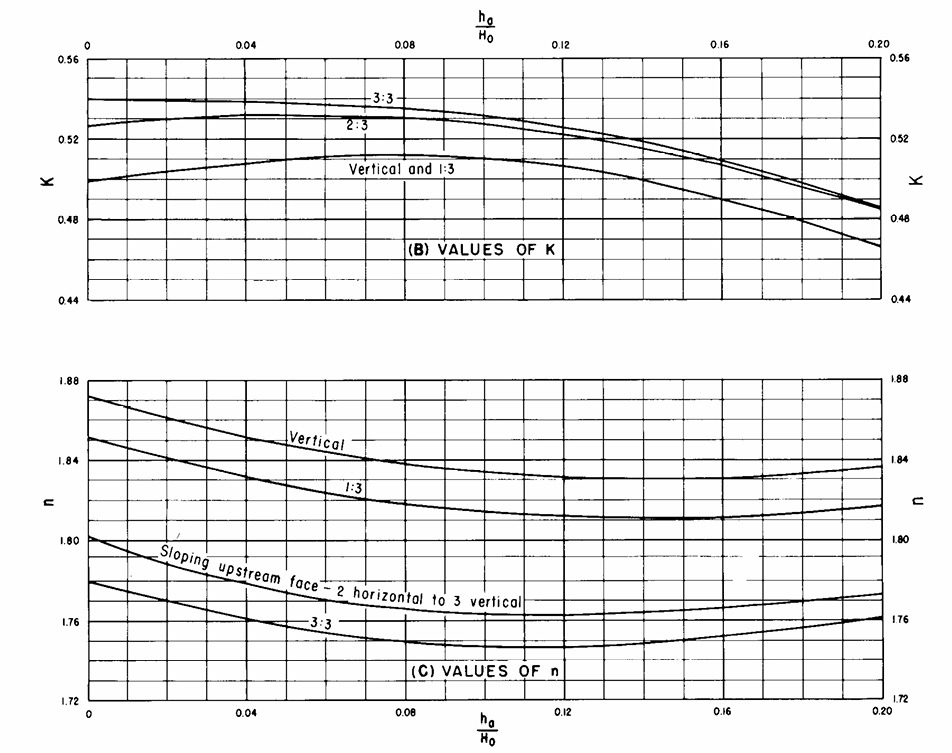
\includegraphics[width=0.85\textwidth]{figures/abaque_kn.jpg}
    \caption{Abaque de détermination des coefficients $K$ et $n$ du profil aval, en fonction de $h_a/H_0$ et de l'inclinaison du parement amont (figure 9-21 -- \textit{Factors for definition of nappe-shaped crest profiles}, planche 288-D-2406, \cite{usbr1987design}).}
    \label{fig:abaque_kn}
\end{figure}

Pour un parement amont vertical, avec $h_a/H_0 \approx 0{,}00204$ et $P/H_0 \approx 9{,}79$, la lecture de l'abaque (figure \ref{fig:abaque_kn}) donne :

\begin{equation}
K = 0{,}5 \qquad n = 1{,}872
\label{eq:coeffs_kn_usace}
\end{equation}

Le tableau \ref{tab:coeffs_kn_creager} récapitule ces deux coefficients.

\begin{table}[H]
    \centering
    \caption{Coefficients $K$ et $n$ du profil Creager}
    \label{tab:coeffs_kn_creager}
    \begin{tabular}{|c|c|c|}
        \hline
        \textbf{Coefficient} & \textbf{Valeur} & \textbf{Unité} \\
        \hline
        $K$ & 0,5 & sans dimension \\
        \hline
        $n$ & 1,872 & sans dimension \\
        \hline
    \end{tabular}
\end{table}

\subsubsection{Coordonnées du point de raccordement seuil-coursier $(X_c,Y_c)$}
\label{subsubsec:coord_xc_yc}

\begin{figure}[H]
    \centering
    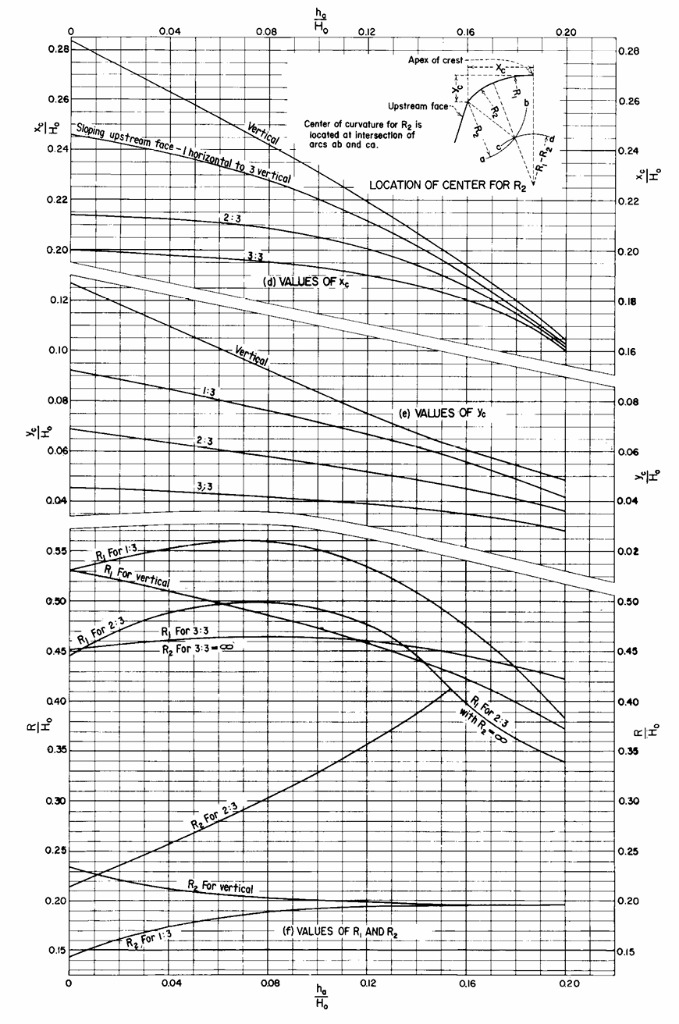
\includegraphics[width=0.85\textwidth]{figures/abaque_Xc_Yc.jpeg}
    \caption{Les paramètres caractéristiques de la partie amont du profil Creager (figure 9-21 -- \textit{Factors for definition of nappe-shaped crest profiles}, planche 288-D-2407, \cite{usbr1987design}).}
    \label{fig:abaque_xc_yc}
\end{figure}

D'après l'abaque (figure \ref{fig:abaque_xc_yc}), pour un parement amont vertical :

\begin{equation}
\frac{X_c}{H_0} = 0{,}283 \;\Rightarrow\; X_c = 0{,}283 \times 2{,}86 \approx 0{,}80652 \text{ m}
\label{eq:coord_xc}
\end{equation}

\begin{equation}
\frac{Y_c}{H_0} = 0{,}126 \;\Rightarrow\; Y_c = 0{,}126 \times 2{,}86 \approx 0{,}3603 \text{ m}
\label{eq:coord_yc}
\end{equation}

\subsubsection{Rayons de raccordement amont et aval $R_1$, $R_2$}
\label{subsubsec:rayons_r1_r2}

D'après l'abaque (figure \ref{fig:abaque_xc_yc}) :

\begin{equation}
\frac{R_1}{H_0} = 0{,}53 \;\Rightarrow\; R_1 = 0{,}53 \times 2{,}86 \approx 1{,}51 \text{ m}
\label{eq:rayon_r1}
\end{equation}

\begin{equation}
\frac{R_2}{H_0} = 0{,}233 \;\Rightarrow\; R_2 = 0{,}233 \times 2{,}86 \approx 0{,}6721 \text{ m}
\label{eq:rayon_r2}
\end{equation}

\subsubsection{Tableau récapitulatif des paramètres du seuil}
\label{subsubsec:recap_profil_usace}

Le tableau \ref{tab:recap_profil_usace} récapitule l'ensemble des paramètres géométriques ainsi obtenus.

\begin{table}[H]
    \centering
    \caption{Récapitulatif des paramètres géométriques du profil Creager ($H_0=2{,}86$ m)}
    \label{tab:recap_profil_usace}
    \begin{tabular}{|c|c|c|c|}
        \hline
        \textbf{Paramètre} & \textbf{Rapport} & \textbf{Valeur du rapport} & \textbf{Valeur (m)} \\
        \hline
        $X_c$ & $X_c/H_0$ & 0,283 & 0,80652 \\
        \hline
        $Y_c$ & $Y_c/H_0$ & 0,126 & 0,3603 \\
        \hline
        $R_1$ & $R_1/H_0$ & 0,53 & 1,51 \\
        \hline
        $R_2$ & $R_2/H_0$ & 0,233 & 0,6721 \\
        \hline
    \end{tabular}
\end{table}

\subsubsection{Équation du profil retenu}
\label{subsubsec:equation_profil_usace}

Avec les coefficients $K=0{,}5$ et $n=1{,}872$ (équation \ref{eq:coeffs_kn_usace}), le profil aval s'écrit, sous forme adimensionnelle (équation \ref{eq:creager_general_kn}) :

\begin{equation}
\frac{Y}{H_0} = -0{,}5 \left(\frac{X}{H_0}\right)^{1{,}872}
\label{eq:profil_creager_hnphe_forme}
\end{equation}

soit, numériquement, avec $H_0=2{,}86$ m :

\begin{equation}
Y = -0{,}5 \times 2{,}86 \times \left(\frac{X}{2{,}86}\right)^{1{,}872} = -1{,}43 \left(\frac{X}{2{,}86}\right)^{1{,}872}
\label{eq:profil_creager_hnphe}
\end{equation}

Le signe négatif de l'équation \ref{eq:profil_creager_hnphe} correspond à un axe $Y$ orienté vers le haut, l'origine étant prise à la crête du seuil ($X=Y=0$) : les points du profil, situés sous la crête, ont donc une ordonnée $Y<0$. L'équation \ref{eq:profil_creager_hnphe} est valable depuis la crête ($X=0$) jusqu'au point de raccordement avec le coursier $(X_c,Y_c) = (0{,}80652\,;\,0{,}3603)$ m (équations \ref{eq:coord_xc}-\ref{eq:coord_yc}).

\subsubsection{Tableau de points pour le tracé de la courbe}
\label{subsubsec:points_profil_usace}

Pour un tracé précis de la courbe, le tableau \ref{tab:points_profil_creager_hnphe} fournit les coordonnées $(X,Y)$ calculées par l'équation \ref{eq:profil_creager_hnphe}, pour $X$ variant de 0 à 2,8 m par pas de 0,1 m, soit l'intervalle couvrant le seuil jusqu'au-delà du point de raccordement $X_c=0{,}80652$ m.

\begin{table}[H]
    \centering
    \caption{Points de la courbe du profil Creager ($H_0=2{,}86$ m, équation \ref{eq:profil_creager_hnphe})}
    \label{tab:points_profil_creager_hnphe}
    \begin{tabular}{|c|c||c|c||c|c|}
        \hline
        \textbf{$X$ (m)} & \textbf{$Y$ (m)} & \textbf{$X$ (m)} & \textbf{$Y$ (m)} & \textbf{$X$ (m)} & \textbf{$Y$ (m)} \\
        \hline
        0 & 0 & 1,0 & -0,20000000 & 2,0 & -0,73207933 \\
        \hline
        0,1 & -0,00268553 & 1,1 & -0,23906561 & 2,1 & -0,80209261 \\
        \hline
        0,2 & -0,00983010 & 1,2 & -0,28135672 & 2,2 & -0,87507495 \\
        \hline
        0,3 & -0,02099911 & 1,3 & -0,32683755 & 2,3 & -0,95100873 \\
        \hline
        0,4 & -0,03598208 & 1,4 & -0,37547556 & 2,4 & -1,02987719 \\
        \hline
        0,5 & -0,05463889 & 1,5 & -0,42724091 & 2,5 & -1,11166438 \\
        \hline
        0,6 & -0,07686509 & 1,6 & -0,48210607 & 2,6 & -1,19635509 \\
        \hline
        0,7 & -0,10257783 & 1,7 & -0,54004553 & 2,7 & -1,28393478 \\
        \hline
        0,8 & -0,13170870 & 1,8 & -0,60103550 & 2,8 & -1,37438951 \\
        \hline
        0,9 & -0,16419955 & 1,9 & -0,66505373 & & \\
        \hline
    \end{tabular}
\end{table}

\subsection{Tracé géométrique du profil sous AutoCAD}
\label{subsec:trace_autocad}

Le tracé du profil de l'évacuateur sous AutoCAD est mené à partir des résultats des calculs théoriques, selon la méthodologie en quatre étapes successives suivante :
\begin{enumerate}
    \item \textbf{Tracé des deux cercles de raccordement amont et aval ($R_1$ et $R_2$)} : La partie amont du profil comprend deux arcs de cercle. Le rayon amont $R_1 = 1{,}51$ m assure le raccordement tangentiel entre le parement amont vertical et la crête du seuil. Le rayon aval $R_2 = 0{,}6721$ m assure le raccordement entre la crête et le début du profil parabolique Creager.
    \item \textbf{Tracé du seuil de l'évacuateur} : Le seuil est tracé point par point à partir de l'équation parabolique adimensionnelle du profil Creager (équation \ref{eq:profil_creager_hnphe}) et des coordonnées définies (tableau \ref{tab:points_profil_creager_hnphe}). Ce tracé s'étend depuis la crête ($X=0, Y=0$) jusqu'au point de raccordement avec le coursier $(X_c,Y_c) = (0{,}80652\,;\,0{,}3603)$ m.
    \item \textbf{Tracé du coursier (partie rectiligne)} : Le coursier est une ligne droite débutant au point de raccordement $(X_c,Y_c)$ avec une pente de $0{,}8$ H pour $1$ V (angle d'inclinaison par rapport à l'horizontale $\alpha \approx 51{,}34^\circ$).
    L'angle d'inclinaison est obtenu par :
    \begin{equation}
    \alpha = \arctan\left(\frac{1}{0{,}8}\right) \approx 51{,}34^\circ
    \label{eq:angle_coursier}
    \end{equation}
    L'équation de cette droite s'écrit :
    \begin{equation}
    Y = 1{,}25\,X - 0{,}64785
    \label{eq:droite_coursier}
    \end{equation}
    Le coursier se prolonge vers l'aval jusqu'au départ de la cuillère, à la cote $586{,}54$ m.
    \item \textbf{Tracé de la cuillère de dissipation (saut de ski)} : La cuillère débute à la cote $586{,}54$ m et se compose d'un arc de cercle de rayon $R_3 = 3$ m se terminant avec un angle de sortie de $\beta = 40^\circ$ orienté vers le haut, le point le plus bas étant calé à la cote de calage de référence $Z_c = 585{,}20$ NGM.
\end{enumerate}

Le tableau \ref{tab:recap_trace_autocad} récapitule l'ensemble des cotes et paramètres géométriques appliqués pour ce tracé géométrique.

\begin{table}[H]
    \centering
    \caption{Récapitulatif des paramètres pour le tracé du profil sous AutoCAD}
    \label{tab:recap_trace_autocad}
    \begin{tabular}{|l|c|c|}
        \hline
        \textbf{Élément} & \textbf{Paramètre} & \textbf{Valeur} \\
        \hline
        Rayon amont & $R_1$ & 1,51 m \\
        \hline
        Rayon aval & $R_2$ & 0,6721 m \\
        \hline
        Point de raccordement (début coursier) & $X_c$ & 0,80652 m \\
        \hline
        Point de raccordement (début coursier) & $Y_c$ & 0,3603 m \\
        \hline
        Équation du seuil & $Y=f(X)$ & $Y=-1{,}43\,(X/2{,}86)^{1{,}872}$ \\
        \hline
        Pente du coursier & $i$ & 0,8 H/V \\
        \hline
        Angle du coursier & $\alpha$ & $\arctan(1{,}25)\approx 51{,}34^\circ$ \\
        \hline
        Équation du coursier & $Y=1{,}25X-0{,}64785$ & -- \\
        \hline
        Début de la cuillère & Cote & 586,54 m \\
        \hline
        Rayon de la cuillère & $R_3$ & 3 m \\
        \hline
        Angle de sortie de la cuillère & $\beta$ & 40° \\
        \hline
    \end{tabular}
\end{table}

La figure \ref{fig:autocad_profil_complet} illustre le tracé géométrique finalisé du profil Creager de l'évacuateur de crues tracé sous AutoCAD avec ses dimensions principales.

\begin{figure}[H]
    \centering
    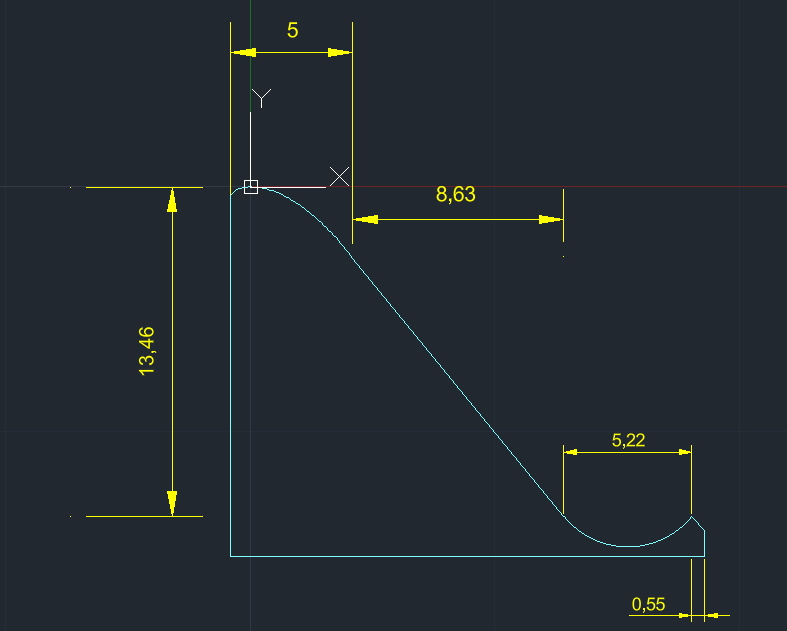
\includegraphics[width=0.85\textwidth]{figures/profil_autocad.png}
    \caption{Tracé géométrique final du profil Creager de l'évacuateur de crues sous AutoCAD avec ses dimensions principales (en mètres).}
    \label{fig:autocad_profil_complet}
\end{figure}

\subsection{La courbe du profil Creager}
\label{subsec:courbe_profil_creager}

La figure \ref{fig:profil_creager} présente la courbe du profil Creager obtenue par application de l'équation \ref{eq:profil_creager_hnphe} (tableau \ref{tab:points_profil_creager_hnphe}), exprimée en cote du radier (NGM). La cote du radier représentée s'en déduit par $\text{Cote} = Z_s + Y$, avec $Z_s = 600{,}00$ NGM (tableau \ref{tab:donnees_base}).

\begin{figure}[H]
    \centering
    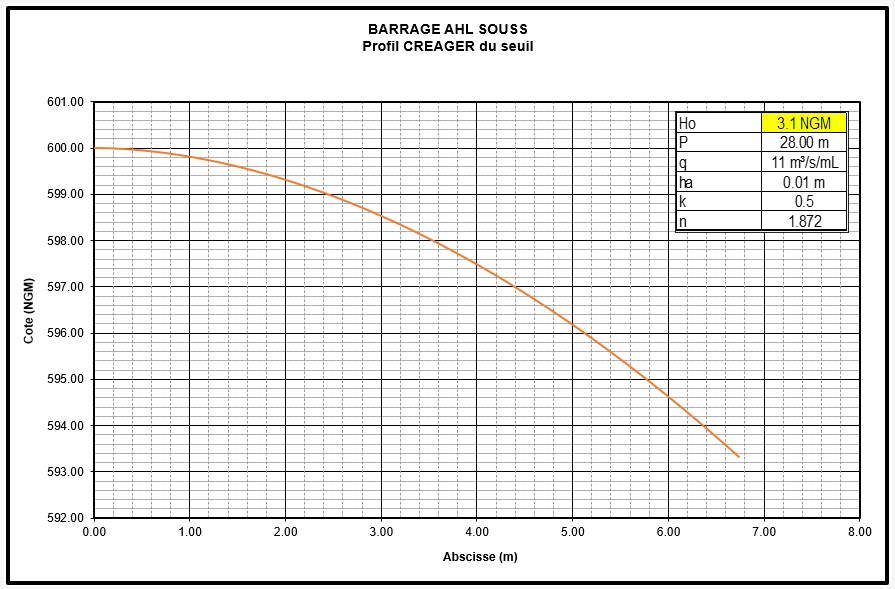
\includegraphics[width=0.85\textwidth]{figures/courbe_profil_creager.png}
    \caption{Courbe du profil Creager de l'évacuateur de crues (origine des abscisses $X=0$ au sommet du seuil ; axe vertical en cote du radier, NGM, décroissante vers l'aval du profil).}
    \label{fig:profil_creager}
\end{figure}



% SECTION : LOI DÉBIT-CHARGE
\section{Loi débit-charge et capacité d'évacuation du seuil}
\label{sec:loi_debit_charge}

La relation générale entre le débit déversé $Q$ et la charge $H$ au-dessus d'un seuil de type Creager s'écrit \cite{usbr1987design, chow1959open} :

\begin{equation}
Q = C \cdot L \cdot H^{3/2}
\label{eq:debit_seuil}
\end{equation}

où $C$ est le coefficient de débit, $L = 70$ m la longueur déversante du seuil (tableau \ref{tab:donnees_base}) et $H$ la charge mesurée au-dessus de la cote du seuil ($Z_s = 600{,}00$ NGM).

Le coefficient $C$ n'est pas constant : il dépend du rapport $H/H_d$ entre la charge effective et la charge de dimensionnement, selon des abaques établis expérimentalement par l'USBR \cite{usbr1987design}. Pour $H = H_d$, $C$ atteint sa valeur de dimensionnement $C_d = 2{,}15$ (tableau \ref{tab:donnees_base}) ; pour $H < H_d$, $C$ est légèrement inférieur à $C_d$ ; pour $H > H_d$, $C$ peut légèrement le dépasser.

\textbf{Vérification à partir des données NPHE.} En exploitant les valeurs de charge et de débit sous NPHE données au chapitre \ref{chap:barrage} ($H_{NPHE} = 2{,}86$ m pour $Q_{NPHE} = 730$ m³/s, soit $H_{NPHE}/H_d \approx 2{,}86/3{,}0677 \approx 0{,}93$), le coefficient de débit correspondant vaut :

\begin{equation}
C = \frac{Q_{NPHE}}{L \cdot H_{NPHE}^{3/2}} = \frac{730}{70 \times 2{,}86^{1,5}} \approx 2{,}16
\label{eq:coeff_debit_verif}
\end{equation}

Cette valeur est très proche du coefficient de dimensionnement $C_d = 2{,}15$ retenu pour la présente étude, l'écart résiduel s'expliquant par le fait que $Q_{NPHE}$ et $H_{NPHE}$ proviennent de la note de calcul initiale (chapitre \ref{chap:barrage}) tandis que $L$ et $H_d$ correspondent aux valeurs affinées de la présente étude. Cette concordance confirme la validité de la loi débit-charge retenue.

\textbf{Détermination de la charge pour chaque débit de crue.} La charge $H$ correspondant à chacun des débits laminés retenus (tableau \ref{tab:debits_lamines}) est obtenue par résolution itérative de l'équation \ref{eq:debit_seuil}, le coefficient $C$ dépendant lui-même de $H$ via le rapport $H/H_d$ (procédure de calcul implémentée dans la feuille de calcul développée pour cette étude) :
\begin{enumerate}
    \item Initialiser $C = C_d$ (valeur de dimensionnement) ;
    \item Calculer $H = (Q / (C \cdot L))^{2/3}$ ;
    \item Mettre à jour $C$ à partir du rapport $H/H_d$ et de l'abaque USBR ;
    \item Répéter les étapes 2 et 3 jusqu'à convergence.
\end{enumerate}

Les résultats de cette procédure sont reportés dans le tableau \ref{tab:loi_debit_charge} et représentés graphiquement à la figure \ref{fig:courbe_debit_charge}.

\begin{table}[H]
    \centering
    \caption{Loi débit-charge du seuil déversant pour les débits laminés retenus}
    \label{tab:loi_debit_charge}
    \begin{tabular}{|c|c|c|c|c|c|}
        \hline
        \textbf{Période de retour (ans)} & \textbf{$Q$ (m³/s)} & \textbf{$H/H_d$} & \textbf{$C/C_d$} & \textbf{$C$} & \textbf{$H$ (m)} \\
        \hline
        10 & 160,74 & 0,369 & 0,893 & 1,92 & 1,13 \\
        \hline
        100 & 507,54 & 0,756 & 0,969 & 2,08 & 2,32 \\
        \hline
        1\,000 & 794,93 & 1,000 & 1,001 & 2,15 & 3,07 \\
        \hline
    \end{tabular}
\end{table}

\begin{figure}[H]
    \centering
    \begin{tikzpicture}
    \begin{axis}[
        width=0.85\textwidth,
        height=7cm,
        xlabel={$H$ (m)},
        ylabel={$Q$ (m\textsuperscript{3}/s)},
        grid=major,
        legend pos=north west,
        legend style={font=\small},
    ]
    \addplot[thick, blue] table[x=H,y=Q] {data/evc_qh.dat};
    \addlegendentry{Loi débit-charge $Q=f(H)$}
    \addplot[only marks, mark=*, mark size=2.5pt, red] coordinates {(1.13183498225396,160.735240718924) (2.31784974886398,507.535888342577) (3.06731336836435,794.925467002904)};
    \addlegendentry{$Q_{10}$, $Q_{100}$, $Q_{1000}$}
    \end{axis}
    \end{tikzpicture}
    \caption{Courbe débit-charge du seuil déversant de l'évacuateur de crues, avec les points correspondant aux trois débits laminés retenus.}
    \label{fig:courbe_debit_charge}
\end{figure}

% SECTION : COURBE DE REMOUS
\section{Calcul de la courbe de remous sur le coursier}
\label{sec:courbe_remous}

\subsection{Principe de la méthode pas-à-pas}
\label{subsec:principe_methode_pas_a_pas}

Le coursier de l'évacuateur de crues est un canal à forte pente sur lequel l'écoulement, critique au voisinage de la crête du seuil, devient rapidement torrentiel (régime supercritique). La détermination du profil de la ligne d'eau le long du coursier relève du calcul des écoulements graduellement variés, régi par l'équation différentielle \cite{chow1959open} :

\begin{equation}
\frac{dy}{dx} = \frac{S_0 - S_f}{1 - Fr^2}
\label{eq:gvf}
\end{equation}

où $y$ est la profondeur d'écoulement, $x$ l'abscisse le long du coursier, $S_0$ la pente du radier, $S_f$ la pente de la ligne d'énergie (perte de charge unitaire) et $Fr$ le nombre de Froude, défini par :

\begin{equation}
Fr = \frac{V}{\sqrt{g \, y}}
\label{eq:froude}
\end{equation}

La pente de frottement $S_f$ (pente de la ligne d'énergie) est évaluée à l'aide de la formule de Manning-Strickler :

\begin{equation}
S_f = \left(\frac{V}{K_s \, R_h^{2/3}}\right)^2
\label{eq:manning_strickler}
\end{equation}

avec $V$ la vitesse moyenne, $R_h$ le rayon hydraulique et $K_s$ le coefficient de Strickler du coursier, pris égal à $K_s = 70$ m$^{1/3}$/s pour un coursier en béton lisse (tableau \ref{tab:donnees_base}).

\subsection{Application au coursier de l'évacuateur de crues}
\label{subsec:application_courbe_remous}

La méthode pas-à-pas (ou méthode par tronçons) consiste à discrétiser le coursier en une succession de sections espacées d'un pas $\Delta x$, et à appliquer entre deux sections consécutives $i$ et $i+1$ l'équation de l'énergie :

\begin{equation}
Z_i + y_i + \frac{V_i^2}{2g} = Z_{i+1} + y_{i+1} + \frac{V_{i+1}^2}{2g} + \overline{S_f}\,\Delta x
\label{eq:energie_pas_a_pas}
\end{equation}

où $Z_i$ désigne la cote du radier à la section $i$ et $\overline{S_f}$ la pente de perte de charge moyenne entre les sections $i$ et $i+1$.

Le calcul est initialisé à la crête du seuil, où la profondeur correspond à la profondeur critique associée au débit considéré, puis mené de proche en proche vers l'aval (le calcul en régime supercritique progresse naturellement depuis l'amont vers l'aval). Cette procédure a été implémentée dans une feuille de calcul, pour chacun des trois débits laminés retenus (tableau \ref{tab:debits_lamines}).

Cette procédure fournit, pour chacun des trois débits laminés étudiés, l'ensemble des points $(x, Z, y, V, E, Fr)$ le long du coursier ; le détail de ces résultats est reporté en annexe, et l'ensemble des points calculés sert à tracer les profils de la figure \ref{fig:profil_ligne_eau}.

\begin{figure}[H]
    \centering
    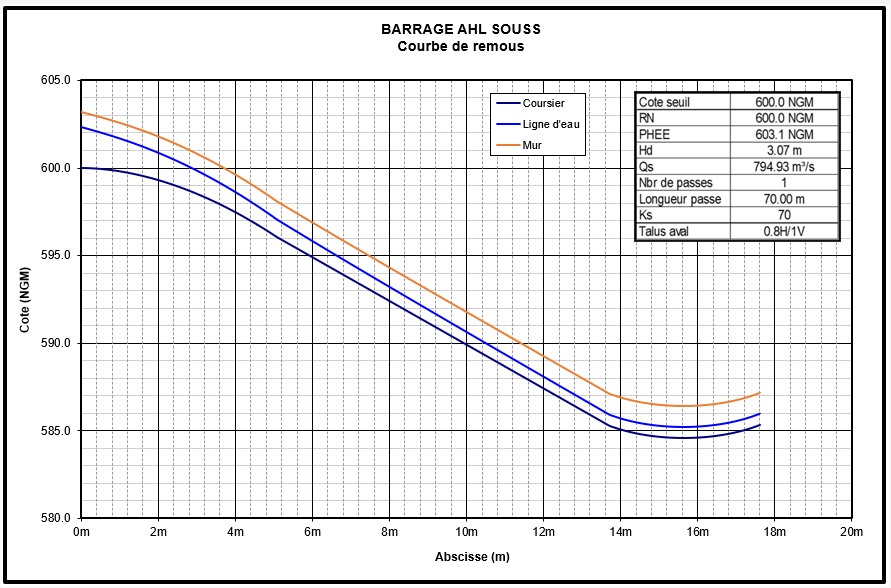
\includegraphics[width=0.85\textwidth]{figures/courbe_remous.png}
    \caption{Courbe de remous calculée par la méthode pas-à-pas, depuis la crête du seuil, pour le débit millénal laminé $Q_{1000} = 794{,}93$ m³/s : profil du radier, ligne d'eau et hauteur du mur bajoyer.}
    \label{fig:profil_ligne_eau}
\end{figure}

% SECTION : HAUTEUR DES MURS BAJOYERS
\section{Détermination de la hauteur des murs bajoyers}
\label{sec:murs_bajoyers}

\subsection{Présentation de l'outil HEC-RAS}
\label{subsec:presentation_hecras}

HEC-RAS (\textit{Hydrologic Engineering Center -- River Analysis System}) est un logiciel développé par le \textit{US Army Corps of Engineers}, largement utilisé en ingénierie hydraulique pour la modélisation unidimensionnelle (1D) et bidimensionnelle (2D) des écoulements à surface libre \cite{usace2016hecras}. Il permet de calculer le profil de la ligne d'eau en régime permanent (\textit{Steady Flow Analysis}) ou transitoire (\textit{Unsteady Flow Analysis}) le long d'un cours d'eau ou d'un ouvrage hydraulique, à partir d'une géométrie définie par une succession de sections transversales.

Le moteur de calcul de HEC-RAS repose sur la méthode du pas-à-pas standard (\textit{standard step method}), fondée sur la même équation de l'énergie que celle présentée à la section \ref{sec:courbe_remous} \cite{usace2016hecras, chow1959open}. Il est capable de traiter les régimes fluvial, torrentiel et mixte, ce qui le rend particulièrement adapté à l'étude des coursiers d'évacuateurs de crues, où l'écoulement transite du régime critique (à la crête) au régime torrentiel (sur le coursier).

Dans le cadre de cette étude, HEC-RAS est utilisé pour modéliser l'écoulement le long du coursier de l'évacuateur de crues et fournir, pour chaque débit de crue, le profil de la ligne d'eau servant de base à la détermination de la hauteur des murs bajoyers. Les résultats de cette modélisation 1D constituent également un second élément de comparaison avec les résultats de la modélisation OpenFOAM (chapitre \ref{chap:resultats_simulation}), en complément de la méthode pas-à-pas sous Excel (section \ref{sec:courbe_remous}).

\subsection{Modélisation 1D du coursier sous HEC-RAS}
\label{subsec:modelisation_hecras}

La géométrie du coursier a été introduite dans HEC-RAS sous la forme d'une succession de sections transversales (\textit{cross-sections}), espacées régulièrement le long de l'axe d'écoulement et établies à partir du profil type de l'ouvrage (profil AutoCAD / SketchUp, cf. section \ref{sec:sketchup}). Pour chaque section, les paramètres suivants ont été renseignés :
\begin{itemize}
    \item La géométrie transversale (largeur du coursier $b$ et géométrie des murs bajoyers) ;
    \item La cote du radier $Z$, déduite du profil Creager (section \ref{sec:profil_seuil}) puis de la pente du coursier ;
    \item Le coefficient de rugosité de Manning $n$, associé à la nature du revêtement en béton du coursier.
\end{itemize}

Le régime d'écoulement étant torrentiel sur l'ensemble du coursier, la condition aux limites amont est fixée à la profondeur critique au niveau de la crête du seuil, et le calcul est mené en régime \textit{supercritique} (option \textit{Mixed} de HEC-RAS, qui permet de basculer automatiquement entre régimes si nécessaire). Une analyse en régime permanent (\textit{Steady Flow Analysis}) est réalisée séparément pour chacun des trois débits laminés retenus (tableau \ref{tab:debits_lamines}), ce qui permet d'obtenir, pour chaque débit, le profil complet de la ligne d'eau le long du coursier.

\begin{figure}[H]
    \centering
    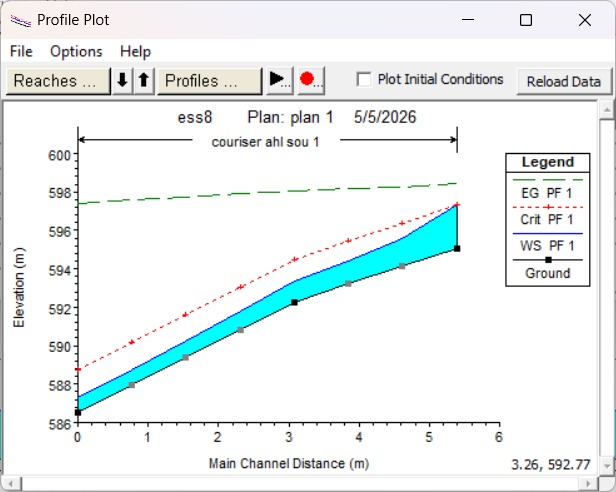
\includegraphics[width=0.6\textwidth]{figures/hecras_profile_plot.jpeg}
    \caption{Profil en long de la ligne d'eau du coursier obtenu sous HEC-RAS (\textit{Profile Plot}) : profil du radier (\textit{Ground}), ligne d'eau (\textit{WS PF 1}) et ligne d'énergie (\textit{EG PF 1}).}
    \label{fig:hecras_profil}
\end{figure}

\subsection{Hauteur des murs bajoyers retenue}
\label{subsec:hauteur_murs_retenue}

La hauteur des murs bajoyers $H_{mur}$ doit permettre de contenir la lame d'eau en écoulement sur le coursier, tout en intégrant une revanche $R_v$ destinée à couvrir les phénomènes non pris en compte par le calcul 1D (entraînement d'air et foisonnement de la lame d'eau, vagues et ondes de choc obliques, incertitudes sur la rugosité) :

\begin{equation}
H_{mur} = y_{max} + R_v
\label{eq:hauteur_mur}
\end{equation}

où $y_{max}$ est la profondeur d'eau maximale le long du coursier pour le débit considéré, obtenue par la méthode pas-à-pas (section \ref{sec:courbe_remous}) et confirmée par la modélisation HEC-RAS. Dans les trois cas étudiés, la profondeur maximale est obtenue dès la crête du seuil ($X=0$), où la lame d'eau est encore peu accélérée, avant de diminuer rapidement le long du coursier (figure \ref{fig:profil_ligne_eau}).

\subsubsection{Calcul de la revanche $R_v$}
\label{subsubsec:calcul_revanche}

La revanche $R_v$ est destinée à couvrir les phénomènes non pris en compte par le calcul 1D (entraînement d'air et foisonnement de la lame d'eau, vagues et ondes de choc obliques, incertitudes sur la rugosité). Elle est calculée, dans la feuille de calcul, à l'aide de la formule empirique suivante \cite{usbr1987design}, fonction de la vitesse moyenne $V$ et de la profondeur d'écoulement $y$ au point de hauteur maximale (crête du seuil, $X=0$) :

\begin{equation}
R_v = 0{,}61 + 0{,}037 \, V \, y^{1/3}
\label{eq:revanche}
\end{equation}

avec $V$ en m/s et $y$ en m. Cette relation traduit l'augmentation de la revanche avec la vitesse d'écoulement : plus le coursier est rapide, plus l'entraînement d'air et le foisonnement de la lame d'eau sont importants, et plus la revanche nécessaire est grande. Le tableau \ref{tab:revanche} présente, pour chacun des trois débits laminés retenus, les valeurs de $V$ et $y$ au point de hauteur maximale ainsi que la revanche $R_v$ qui en résulte.

\begin{table}[H]
    \centering
    \caption{Calcul de la revanche $R_v$ au point de hauteur maximale (crête du seuil)}
    \label{tab:revanche}
    \begin{tabular}{|c|c|c|c|c|}
        \hline
        \textbf{Période de retour (ans)} & \textbf{$Q$ (m³/s)} & \textbf{$y$ (m)} & \textbf{$V$ (m/s)} & \textbf{$R_v$ (m)} \\
        \hline
        10 & 160,74 & 1,10 & 2,82 & 0,72 \\
        \hline
        100 & 507,54 & 1,60 & 4,14 & 0,79 \\
        \hline
        1\,000 & 794,93 & 2,00 & 4,81 & 0,83 \\
        \hline
    \end{tabular}
\end{table}

Le tableau \ref{tab:hauteur_murs} synthétise, pour chacun des trois débits laminés retenus (tableau \ref{tab:debits_lamines}), la profondeur maximale $y_{max}$, la revanche $R_v$ et la hauteur de mur bajoyer $H_{mur}$ qui en résulte. La valeur enveloppe, obtenue pour $Q_{1000}$, est retenue comme hauteur de mur bajoyer de référence pour l'ensemble du coursier : $H_{mur} \approx 2{,}83$ m.

\begin{table}[H]
    \centering
    \caption{Détermination de la hauteur des murs bajoyers}
    \label{tab:hauteur_murs}
    \begin{tabular}{|c|c|c|c|c|}
        \hline
        \textbf{Période de retour (ans)} & \textbf{$Q$ (m³/s)} & \textbf{$y_{max}$ (m)} & \textbf{$R_v$ (m)} & \textbf{$H_{mur}$ (m)} \\
        \hline
        10 & 160,74 & 1,10 & 0,72 & 1,82 \\
        \hline
        100 & 507,54 & 1,60 & 0,79 & 2,39 \\
        \hline
        1\,000 & 794,93 & 2,00 & 0,83 & 2,83 \\
        \hline
    \end{tabular}
\end{table}

À titre de comparaison, la feuille de calcul Excel développée pour la courbe de remous calcule également, section par section le long du coursier et pour le débit millénal laminé $Q_{1000}$, une hauteur de mur bajoyer égale à la profondeur d'écoulement $y$ majorée d'une revanche forfaitaire ; le maximum ainsi obtenu, atteint dès la crête du seuil, est de $2{,}00$ m, soit la valeur de $y_{max}$ retenue ci-dessus. La hauteur $H_{mur} \approx 2{,}83$ m (tableau \ref{tab:hauteur_murs}), qui intègre la revanche $R_v$ déterminée à partir de la formule \ref{eq:revanche}, demeure l'enveloppe retenue comme hauteur de référence pour le dimensionnement des murs bajoyers.

Le tableau \ref{tab:extrait_remous_mur} présente un extrait de ce calcul section par section pour $Q_{1000} = 794{,}93$ m³/s, illustrant l'évolution des grandeurs hydrauliques et de la hauteur de mur le long du coursier.

\begin{table}[H]
    \centering
    \caption{Extrait du calcul de la hauteur des murs bajoyers section par section (courbe de remous Excel, $Q_{1000} = 794{,}93$ m³/s)}
    \label{tab:extrait_remous_mur}
    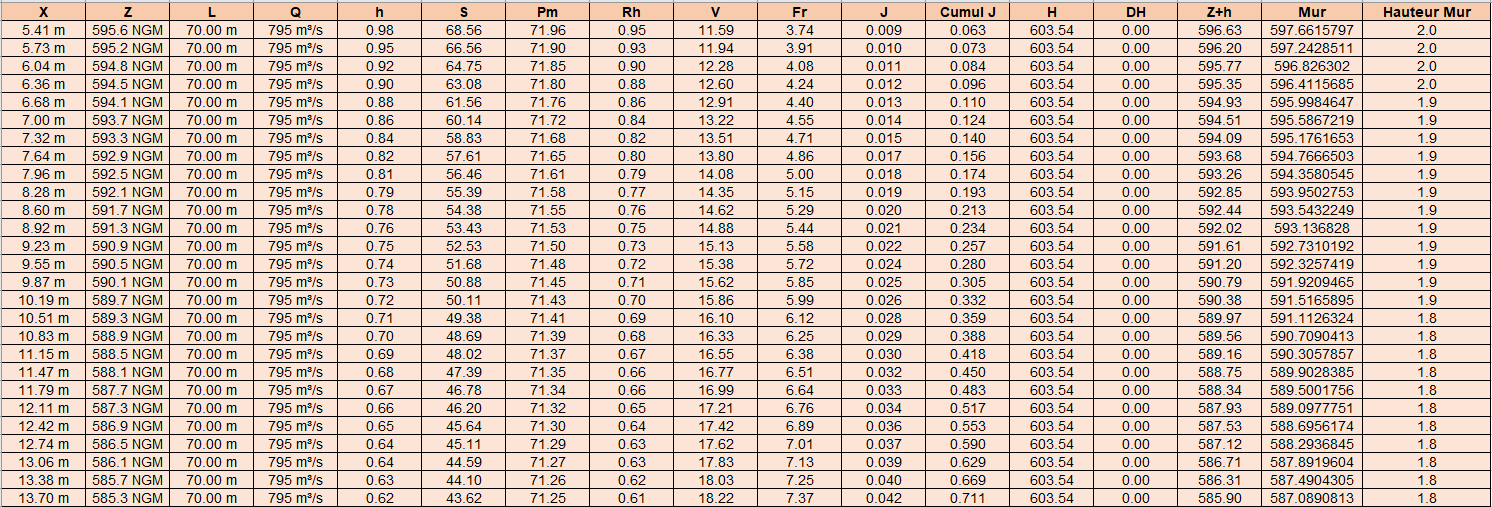
\includegraphics[width=\textwidth]{figures/tableau_mur_bajoyer_excel.png}
\end{table}

\paragraph{Comparaison des résultats Excel et HEC-RAS pour $Q_{1000}$}

Les deux approches appliquent la même formule de revanche USBR (équation \ref{eq:revanche}) pour $Q_{1000}$. Le tableau \ref{tab:comparaison_mur_excel_hecras} compare les hauteurs maximales obtenues.

\begin{table}[H]
    \centering
    \caption{Comparaison des hauteurs maximales de mur bajoyer, revanche incluse — calcul Excel et HEC-RAS ($Q_{1000} = 794{,}93$ m³/s)}
    \label{tab:comparaison_mur_excel_hecras}
    \begin{tabular}{|l|c|}
        \hline
        \textbf{Méthode} & \textbf{$H_{mur,max}$ (m)} \\
        \hline
        Calcul Excel section par section (colonne \og Hauteur Mur \fg{}, revanche incluse) & $2{,}00$ \\
        \hline
        Modélisation HEC-RAS : $H_{mur} = y_{max} + R_v = 2{,}00 + 0{,}83$ & $2{,}83$ \\
        \hline
        \textbf{Écart} $\Delta H$ & $\mathbf{0{,}83}$ \\
        \hline
    \end{tabular}
\end{table}

L'écart $\Delta H = 2{,}83 - 2{,}00 = 0{,}83$ m est égal à la revanche $R_v$ :

\[
R_v = 0{,}61 + 0{,}037 \times 4{,}81 \times 2{,}00^{1/3} = 0{,}83 \text{ m}
\]

La feuille de calcul Excel évalue la hauteur de mur section par section en intégrant la revanche à chaque pas via la même formule USBR, et retient le maximum sur l'ensemble du coursier, soit $H_{mur}^{\text{Excel}} = 2{,}00$ m. La modélisation HEC-RAS, quant à elle, construit la hauteur de mur à partir de la profondeur maximale enveloppe $y_{max} = 2{,}00$ m à laquelle elle ajoute explicitement $R_v = 0{,}83$ m, donnant $H_{mur}^{\text{HEC-RAS}} = 2{,}83$ m. C'est cette dernière valeur qui est retenue comme hauteur de référence pour le dimensionnement des murs bajoyers, car elle représente la condition la plus défavorable sur l'ensemble du coursier.

% SECTION : GÉOMÉTRIE DE LA CUILLÈRE
\section{Géométrie de la cuillère (saut de ski)}
\label{sec:geometrie_cuillere}

Le rôle de la cuillère du saut de ski est de dévier le jet d'eau issu du coursier vers le haut, afin de le projeter à distance du pied aval du barrage et de limiter ainsi le risque d'érosion régressive au contact direct de l'ouvrage. La géométrie de la cuillère du barrage Ahl Souss, présentée au chapitre \ref{chap:barrage}, est caractérisée par :
\begin{itemize}
    \item Une cote de calage du point bas de la cuillère $Z_c = 585{,}20$ NGM ;
    \item Un bec déviateur tracé selon un arc de cercle de rayon $R = 3$ m ;
    \item Un angle de sortie $\theta = 40°$ par rapport à l'horizontale.
\end{itemize}

D'un point de vue dimensionnel, le rayon $R$ de la cuillère doit être suffisant pour limiter la pression dynamique exercée sur le radier au point bas de la cuillère, où l'écoulement change brutalement de direction. L'USBR recommande de vérifier que le rapport entre le rayon de courbure et la profondeur d'eau au point de décollement du jet ($R/y_0$) reste supérieur à environ $4$, de manière à éviter les risques de décollement de la lame d'eau et de cavitation sur l'extrados de la cuillère \cite{usbr1987design}.

La profondeur $y_0$ et la vitesse $V_0$ au point de décollement du jet sont obtenues à partir de la dernière section calculée de la courbe de remous (section \ref{sec:courbe_remous}), à la cote $Z_0$ -- un point du profil de la cuillère situé légèrement au-dessus du point bas de calage $Z_c$. Le tableau \ref{tab:geometrie_cuillere} récapitule, pour chacun des trois débits laminés retenus, les conditions d'écoulement au point de décollement du jet ainsi que la vérification du critère $R/y_0$.

\begin{table}[H]
    \centering
    \caption{Conditions d'écoulement au point de décollement du jet et vérification géométrique}
    \label{tab:geometrie_cuillere}
    \begin{tabular}{|c|c|c|c|c|c|c|}
        \hline
        \textbf{Période de retour (ans)} & \textbf{$Q$ (m³/s)} & \textbf{$y_0$ (m)} & \textbf{$V_0$ (m/s)} & \textbf{$Z_0$ (m NGM)} & \textbf{$R/y_0$} & \textbf{Vérification} \\
        \hline
        10 & 160,74 & 0,128 & 17,89 & 583,91 & 23,37 & $R/y_0 > 4$ : OK \\
        \hline
        100 & 507,54 & 0,431 & 16,81 & 586,79 & 6,96 & $R/y_0 > 4$ : OK \\
        \hline
        1\,000 & 794,93 & 0,634 & 17,91 & 585,32 & 4,73 & $R/y_0 > 4$ : OK \\
        \hline
    \end{tabular}
\end{table}

Le critère $R/y_0 > 4$ est vérifié pour les trois débits laminés retenus, avec une marge qui se réduit logiquement lorsque le débit augmente, la profondeur $y_0$ croissant avec $Q$ alors que le rayon $R$ reste fixe. Le débit millénal $Q_{1000}$, le plus défavorable, présente la marge la plus faible ($R/y_0 \approx 4{,}7$), ce qui reste compatible avec le rayon $R = 3$ m retenu pour le bec déviateur.

\begin{figure}[H]
    \centering
    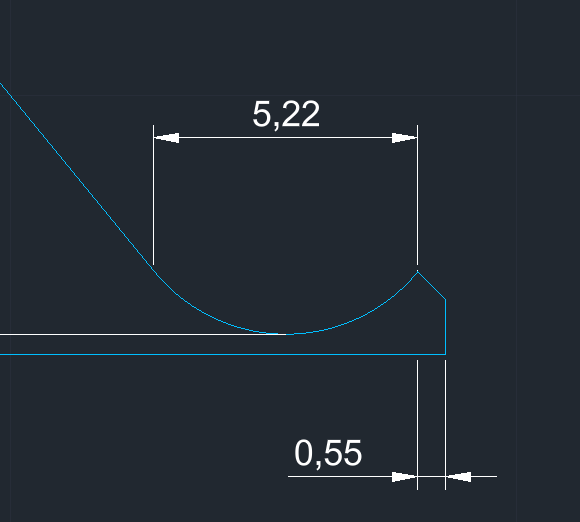
\includegraphics[width=0.65\textwidth]{figures/geometrie_cuillere.png}
    \caption{Géométrie de la cuillère et du bec déviateur du saut de ski.}
    \label{fig:geometrie_cuillere}
\end{figure}

% SECTION : DISTANCE D'IMPACT DU JET
\section{Distance d'impact du jet à l'aval}
\label{sec:distance_impact_jet}

À la sortie du bec déviateur, le jet d'eau quitte la cuillère avec une vitesse $V_0$ et un angle $\theta = 40°$ par rapport à l'horizontale, puis évolue en trajectoire libre jusqu'à son impact sur le terrain naturel ou le lit de l'oued. En prenant pour origine le point de sortie du bec déviateur, avec un axe $x$ horizontal orienté vers l'aval et un axe $z$ vertical orienté vers le haut, et en négligeant la résistance de l'air, la trajectoire du jet s'écrit \cite{usbr1987design} :

\begin{equation}
z(x) = x \tan\theta - \frac{g\,x^2}{2\,V_0^2 \cos^2\theta}
\label{eq:trajectoire_jet}
\end{equation}

Le point d'impact, situé à une dénivelée $\Delta Z = Z_0 - Z_{aval}$ en dessous du point de décollement du jet (avec $Z_{aval} = 579{,}50$ NGM la cote du radier du bassin de dissipation, tableau \ref{tab:donnees_base}), est obtenu en posant $z(x) = -\Delta Z$ dans l'équation \ref{eq:trajectoire_jet}, ce qui conduit, après résolution de l'équation du second degré en $x$, à la distance d'impact $L_x$ :

\begin{equation}
L_x = V_0 \cos\theta \cdot \frac{V_0 \sin\theta + \sqrt{(V_0 \sin\theta)^2 + 2 g \Delta Z}}{g}
\label{eq:distance_impact}
\end{equation}

La vitesse $V_0$ et la cote $Z_0$ au point de décollement du jet sont issues du tableau \ref{tab:geometrie_cuillere} (section \ref{sec:geometrie_cuillere}). Le tableau \ref{tab:distance_impact} présente la distance d'impact $L_x$ obtenue pour chacun des trois débits laminés retenus.

\begin{table}[H]
    \centering
    \caption{Distance d'impact du jet pour les débits laminés retenus}
    \label{tab:distance_impact}
    \begin{tabular}{|c|c|c|c|c|}
        \hline
        \textbf{Période de retour (ans)} & \textbf{$Q$ (m³/s)} & \textbf{$V_0$ (m/s)} & \textbf{$\Delta Z$ (m)} & \textbf{$L_x$ (m)} \\
        \hline
        10 & 160,74 & 17,89 & 4,41 & 36,72 \\
        \hline
        100 & 507,54 & 16,81 & 7,29 & 35,36 \\
        \hline
        1\,000 & 794,93 & 17,91 & 5,82 & 38,07 \\
        \hline
    \end{tabular}
\end{table}

Les valeurs de $L_x$ restent comprises entre 35 et 38 m pour les trois débits étudiés : les variations de $V_0$ et de $\Delta Z$ se compensent partiellement, sans tendance strictement monotone.

La figure \ref{fig:trajectoire_jet} présente la trajectoire du jet obtenue par la modélisation sous tableur Excel pour le débit millénaire $Q_{1000} = 794{,}93$ m³/s, avec les mêmes paramètres que ceux du tableau \ref{tab:distance_impact} (talus aval $= 0{,}8\,\mathrm{H}/1\,\mathrm{V}$, longueur de passe $= 70$ m, PHE $= 603{,}1$ m NGM, PHE\,aval $= 574$ m NGM).

\begin{figure}[H]
    \centering
    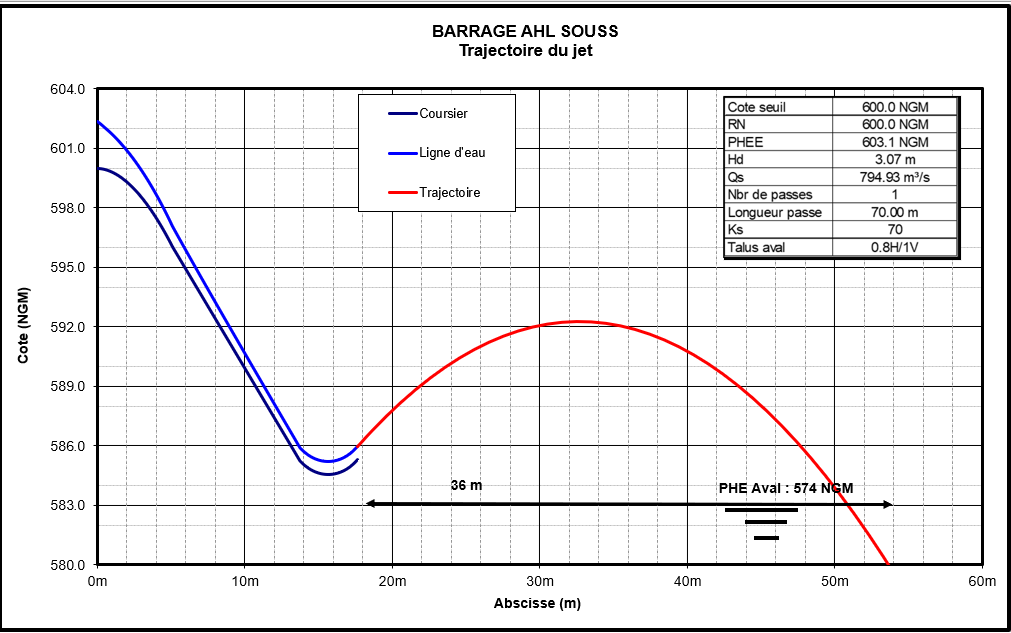
\includegraphics[width=0.92\textwidth]{figures/trajectoire_jet.png}
    \caption{Trajectoire du jet issu de la cuillère saut de ski — Barrage Ahl Souss, $Q_{1000} = 794{,}93$ m³/s (modélisation Excel)}
    \label{fig:trajectoire_jet}
\end{figure}

Le graphe Excel indique une distance d'impact $L_x^{\mathrm{Excel}} \approx 36$ m pour $Q_{1000}$, à comparer avec la valeur analytique $L_x^{\mathrm{calc}} = 38{,}07$ m issue de l'équation \ref{eq:distance_impact}. L'écart entre les deux estimations est de l'ordre de \textbf{5,4\,\%}, ce qui est tout à fait acceptable compte tenu des hypothèses simplificatrices de la trajectoire parabolique (résistance de l'air négligée, angle de décollement fixé à $40°$). Les deux approches confirment que le jet retombe à une distance d'environ 36 à 38 m du pied de la cuillère, bien au-delà du pied aval du barrage, et que sa trajectoire reste compatible avec l'emprise du bassin de dissipation projeté (chapitre \ref{chap:barrage}).

% SECTION : AFFOUILLEMENT
\section{Évaluation de l'affouillement à l'aval du barrage}
\label{sec:affouillement}

L'impact du jet issu du saut de ski sur le lit de l'oued provoque, à long terme, le développement d'une fosse d'érosion (ou fosse d'affouillement) dont la profondeur conditionne la stabilité du pied aval de l'ouvrage et des éventuels dispositifs de protection. Afin d'encadrer cette profondeur, quatre formules empiriques classiques ont été appliquées, chacune basée sur le débit unitaire $q = Q/L$ et une hauteur de chute caractéristique :

\begin{itemize}
    \item $H$ : dénivelée entre la cote PHE et la cote de départ du jet $Z_0$ (cuillère), soit $H = \mathrm{PHE} - Z_0$ ;
    \item $h^*$ : charge totale de chute entre la cote PHE et la cote du lit aval (PHE aval), soit $h^* = \mathrm{PHE} - \mathrm{PHE_{aval}}$.
\end{itemize}

\noindent\textbf{Formule de Veronese} \cite{usbr1987design} :
\begin{equation}
D = 1{,}90 \; q^{0,54} \; H^{0,225}
\label{eq:affouillement_veronese}
\end{equation}

\noindent\textbf{Formule de Damle} :
\begin{equation}
D = 0{,}65 \; q^{0,50} \; (h^*)^{0,50}
\label{eq:affouillement_damle}
\end{equation}

\noindent\textbf{Formule de Martins} :
\begin{equation}
D = 1{,}5 \; q^{0,60} \; H^{0,10}
\label{eq:affouillement_martins}
\end{equation}

\noindent\textbf{Formule de Chian} :
\begin{equation}
D = 1{,}18 \; q^{0,51} \; H^{0,235}
\label{eq:affouillement_chian}
\end{equation}

\noindent où $D$ est la profondeur d'affouillement mesurée sous le niveau du lit aval (m) et $q$ le débit unitaire (m²/s).

\medskip
Les calculs ont été réalisés pour les trois débits de crue retenus. Pour chaque débit, les paramètres $H$ (dénivelée PHE\,--\,départ du jet) et $h^*$ (dénivelée PHE\,--\,PHE\,aval) sont issus du bilan hydraulique du coursier. La cote de fond de fosse est obtenue par : cote\,=\,PHE\,aval\,$- D$, la PHE aval commune étant de 596,19 m NGM.

\subsubsection*{Débit décennal --- $Q_{10} = 161$ m³/s}

\begin{figure}[H]
    \centering
    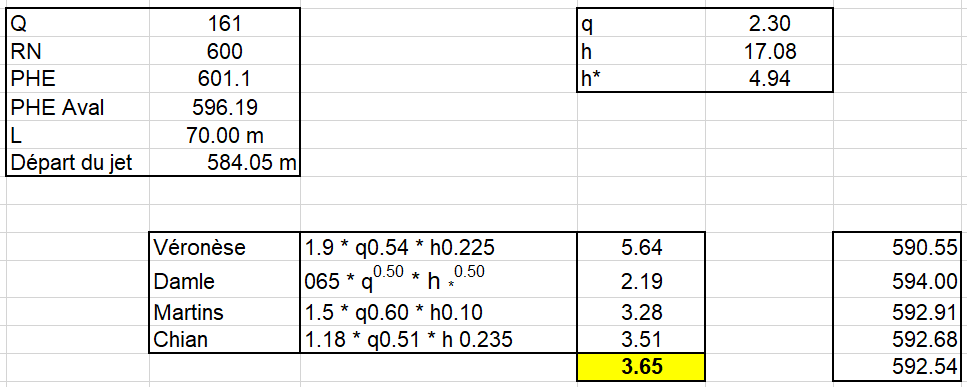
\includegraphics[width=\textwidth]{figures/fosse_q10.png}
    \caption{Calcul de la profondeur d'affouillement pour $Q_{10} = 161$ m³/s ($q = 2{,}30$ m²/s, $H = 17{,}08$ m, $h^* = 4{,}94$ m) — résultats des quatre formules empiriques}
    \label{fig:fosse_q10}
\end{figure}

Pour le débit décennal ($Q_{10} = 161$ m³/s, $q = 2{,}30$ m²/s), les profondeurs d'affouillement calculées varient de 2,19 m (Damle) à 5,64 m (Veronese). La valeur moyenne est $D_{10} = 3{,}65$ m, correspondant à une cote de fond de fosse de $596{,}19 - 3{,}65 = \mathbf{592{,}54}$ m NGM. La faiblesse du débit unitaire pour ce scénario explique les profondeurs modestes obtenues par l'ensemble des formules.

\subsubsection*{Débit centennal --- $Q_{100} = 508$ m³/s}

\begin{figure}[H]
    \centering
    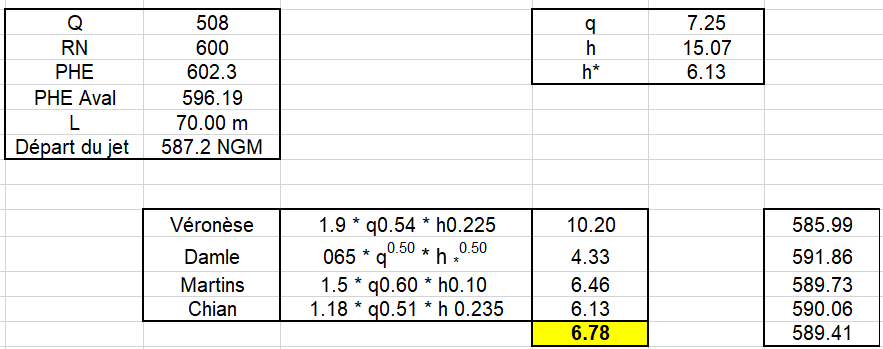
\includegraphics[width=\textwidth]{figures/fosse_q100.png}
    \caption{Calcul de la profondeur d'affouillement pour $Q_{100} = 508$ m³/s ($q = 7{,}25$ m²/s, $H = 15{,}07$ m, $h^* = 6{,}13$ m) — résultats des quatre formules empiriques}
    \label{fig:fosse_q100}
\end{figure}

Pour le débit centennal ($Q_{100} = 508$ m³/s, $q = 7{,}25$ m²/s), les profondeurs obtenues s'étendent de 4,33 m (Damle) à 10,20 m (Veronese). La valeur moyenne est $D_{100} = 6{,}78$ m, pour une cote de fond de fosse de $596{,}19 - 6{,}78 = \mathbf{589{,}41}$ m NGM. La nette augmentation du débit unitaire par rapport à $Q_{10}$ se traduit par un creusement sensiblement plus important.

\subsubsection*{Débit millénaire --- $Q_{1000} = 795$ m³/s}

\begin{figure}[H]
    \centering
    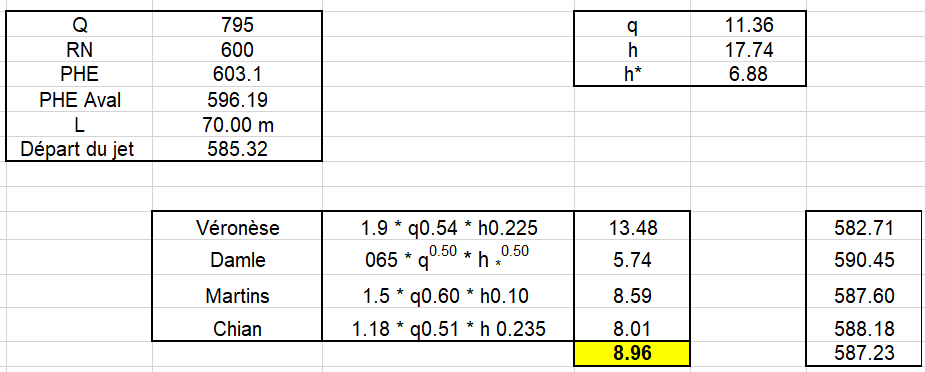
\includegraphics[width=\textwidth]{figures/fosse_q1000.png}
    \caption{Calcul de la profondeur d'affouillement pour $Q_{1000} = 795$ m³/s ($q = 11{,}36$ m²/s, $H = 17{,}74$ m, $h^* = 6{,}88$ m) — résultats des quatre formules empiriques}
    \label{fig:fosse_q1000}
\end{figure}

Pour le débit millénaire ($Q_{1000} = 795$ m³/s, $q = 11{,}36$ m²/s), scénario le plus sévère, les profondeurs calculées s'étalent de 5,74 m (Damle) à 13,48 m (Veronese). La valeur moyenne est $D_{1000} = 8{,}96$ m, soit une cote de fond de fosse de $596{,}19 - 8{,}96 = \mathbf{587{,}23}$ m NGM.

\medskip
Le tableau \ref{tab:affouillement} récapitule l'ensemble des résultats pour les trois débits étudiés :

\begin{table}[H]
    \centering
    \caption{Profondeur d'affouillement $D$ (m) et cote de fond de fosse (m NGM) — comparaison des quatre formules empiriques pour les trois débits de crue (PHE\,aval $= 596{,}19$ m NGM)}
    \label{tab:affouillement}
    \resizebox{\textwidth}{!}{%
    \begin{tabular}{|l|c|c|c|c|c|c|}
        \hline
        \textbf{Formule} & \multicolumn{2}{c|}{$Q_{10} = 161$ m³/s} & \multicolumn{2}{c|}{$Q_{100} = 508$ m³/s} & \multicolumn{2}{c|}{$Q_{1000} = 795$ m³/s} \\
        \hline
        & $D$ (m) & Cote (m NGM) & $D$ (m) & Cote (m NGM) & $D$ (m) & Cote (m NGM) \\
        \hline
        Veronese  & 5,64 & 590,55 & 10,20 & 585,99 & 13,48 & 582,71 \\
        \hline
        Damle     & 2,19 & 594,00 &  4,33 & 591,86 &  5,74 & 590,45 \\
        \hline
        Martins   & 3,28 & 592,91 &  6,46 & 589,73 &  8,59 & 587,60 \\
        \hline
        Chian     & 3,51 & 592,68 &  6,13 & 590,06 &  8,01 & 588,18 \\
        \hline
        \textbf{Moyenne} & \textbf{3,65} & \textbf{592,54} & \textbf{6,78} & \textbf{589,41} & \textbf{8,96} & \textbf{587,23} \\
        \hline
    \end{tabular}}
\end{table}

La profondeur d'affouillement croît avec le débit de crue, passant d'une moyenne de 3,65 m pour $Q_{10}$ à 8,96 m pour $Q_{1000}$. Pour le scénario dimensionnant ($Q_{1000} = 795$ m³/s), la valeur retenue est $D = 8{,}96$ m, correspondant à une cote de fond de fosse de \textbf{587,23 m NGM}. Cette cote reste nettement supérieure aux fondations du barrage, confirmant l'absence de risque direct d'affouillement sur les fondations ; le cas échéant, une protection complémentaire (enrochement, radier aval) pourra être dimensionnée en référence à cette valeur.

% SECTION : SYNTHÈSE DES RÉSULTATS THÉORIQUES
\section{Synthèse des résultats théoriques}
\label{sec:synthese_resultats_theoriques}

Les sections précédentes ont permis d'établir, pour chacun des trois débits laminés étudiés, l'ensemble des grandeurs hydrauliques caractéristiques du fonctionnement de l'évacuateur de crues : charge sur le seuil, profondeur et vitesse d'écoulement le long du coursier, hauteur des murs bajoyers, conditions d'écoulement au niveau de la cuillère, distance d'impact du jet et profondeur d'affouillement. Le tableau \ref{tab:synthese_theorique} regroupe l'ensemble de ces résultats théoriques.

\begin{table}[H]
    \centering
    \caption{Synthèse des résultats théoriques pour les débits laminés retenus}
    \label{tab:synthese_theorique}
    \resizebox{\textwidth}{!}{%
    \begin{tabular}{|c|c|c|c|c|c|c|c|}
        \hline
        \textbf{$T$ (ans)} & \textbf{$Q$ (m³/s)} & \textbf{$H$ (m)} & \textbf{$y_{max}$ coursier (m)} & \textbf{$H_{mur}$ (m)} & \textbf{$V_0$ cuillère (m/s)} & \textbf{$L_x$ (m)} & \textbf{$D$ (m)} \\
        \hline
        10 & 160,74 & 1,13 & 1,10 & 1,82 & 17,89 & 36,72 & 3,65 \\
        \hline
        100 & 507,54 & 2,32 & 1,60 & 2,39 & 16,81 & 35,36 & 6,78 \\
        \hline
        1\,000 & 794,93 & 3,07 & 2,00 & 2,83 & 17,91 & 38,07 & 8,96 \\
        \hline
    \end{tabular}}
\end{table}

Ce tableau récapitulatif constitue la base de comparaison de référence pour l'analyse des résultats de la modélisation numérique sous OpenFOAM, présentée au chapitre \ref{chap:resultats_simulation} (section \ref{sec:comparaison_theorie_numerique}). Pour chaque débit de crue simulé, les grandeurs obtenues numériquement (charge sur le seuil, hauteur d'eau le long du coursier, trajectoire et distance d'impact du jet) seront confrontées aux valeurs théoriques de ce tableau, afin d'évaluer la cohérence du dimensionnement existant et d'identifier d'éventuels écarts entre l'approche 1D/empirique et l'approche tridimensionnelle.

% ============================================================
%  CHAPITRE 8 : Mise en œuvre du cas OpenFOAM
% ============================================================
\chapter{Mise en œuvre du cas OpenFOAM}
\label{chap:mise_en_oeuvre_openfoam}

% SECTION : INTRODUCTION
\section{Introduction}
\label{sec:intro_mise_en_oeuvre}

Après avoir présenté la structure générale d'un code CFD et l'organisation d'un cas OpenFOAM (chapitre \ref{chap:structure_cfd_openfoam}), puis établi le cadre théorique de référence pour l'évacuateur de crues du barrage Ahl Souss (chapitre \ref{chap:dimensionnement_theorique}), ce chapitre décrit la construction concrète du cas de calcul OpenFOAM utilisé pour la modélisation de l'écoulement.

La mise en œuvre du cas suit les étapes classiques d'une étude CFD \cite{greenshields2020openfoam} : préparation de la géométrie et du domaine de calcul (section \ref{sec:preparation_geometrie}), génération du maillage (section \ref{sec:generation_maillage}), définition des conditions initiales et aux limites (section \ref{sec:conditions_limites}), paramétrage du solveur \texttt{interFoam} (section \ref{sec:configuration_solveur}) et enfin lancement des simulations avec suivi de leur convergence (section \ref{sec:lancement_simulations}). Ces différentes étapes ont été répétées pour chacun des trois débits laminés retenus (tableau \ref{tab:debits_lamines}), conformément aux objectifs de l'étude.

% SECTION : PRÉPARATION DE LA GÉOMÉTRIE
\section{Préparation de la géométrie et du domaine de calcul}
\label{sec:preparation_geometrie}

La géométrie du modèle numérique repose sur la chaîne de modélisation présentée au chapitre \ref{chap:benchmark_logiciels} (section \ref{sec:sketchup}) : les profils types 2D de l'évacuateur de crues (profil Creager, coursier, murs bajoyers, cuillère et bec déviateur) ont été réalisés sous \textbf{AutoCAD}, puis importés dans \textbf{SketchUp} pour la construction du modèle tridimensionnel intégrant le terrain naturel (via l'outil \textit{Sandbox}), avant export au format \textbf{STL} grâce à l'extension SketchUp STL \cite{lhuillier2014sketchupstl}.

Le domaine de calcul retenu pour la simulation OpenFOAM se décompose en plusieurs zones fonctionnelles :
\begin{itemize}
    \item Une \textbf{zone amont}, correspondant à une portion de la retenue, suffisamment étendue pour que le niveau d'eau s'y stabilise au niveau imposé par les conditions aux limites et ne soit pas perturbé par l'écoulement sur le seuil ;
    \item La \textbf{zone de l'ouvrage}, comprenant le seuil déversant (profil Creager, section \ref{sec:profil_seuil}), le coursier et ses murs bajoyers, ainsi que la cuillère et le bec déviateur (section \ref{sec:geometrie_cuillere}) ;
    \item Une \textbf{zone aval}, couvrant la trajectoire du jet et sa zone d'impact sur le lit de l'oued, ainsi que la zone potentielle de développement de la fosse d'érosion (section \ref{sec:affouillement}) ; son extension est dimensionnée à partir de la distance d'impact théorique du jet ($L_x \approx 38$ m pour le débit millénal laminé $Q_{1000}$, tableau \ref{tab:distance_impact}), avec une marge suffisante en aval ;
    \item Une \textbf{zone atmosphérique}, au-dessus du plan d'eau, nécessaire à la méthode VOF pour représenter l'interface air-eau (\texttt{alpha.water}) et permettre son évolution libre, y compris en cas de projection ou d'éclaboussures.
\end{itemize}

Chaque composante géométrique (terrain naturel, ouvrage en béton, surfaces de l'évacuateur) est exportée sous la forme d'un fichier STL distinct, placé dans le sous-répertoire \texttt{constant/triSurface} du cas OpenFOAM, conformément à l'organisation présentée au chapitre \ref{chap:structure_cfd_openfoam}. Cette séparation par fichiers permet d'attribuer, lors de la génération du maillage, des conditions de raffinement et des conditions aux limites spécifiques à chaque surface.

\begin{figure}[H]
    \centering
    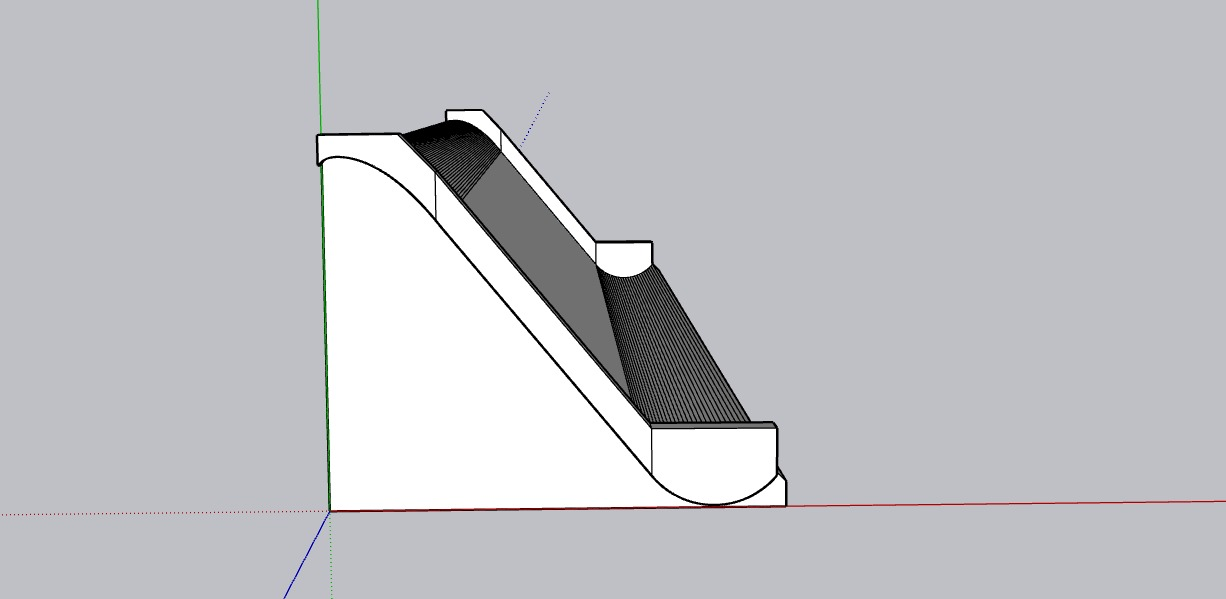
\includegraphics[width=0.85\textwidth]{figures/sketchup_domaine_calcul.jpeg}
    \caption{Modèle 3D SketchUp de l'évacuateur de crues du barrage Ahl Souss : vue en coupe du profil Creager, du coursier et de la cuillère de restitution, utilisé comme base de l'export STL pour la modélisation OpenFOAM.}
    \label{fig:domaine_calcul}
\end{figure}

La longueur totale du domaine de calcul a été fixée à \textbf{70 m}, depuis la face amont du réservoir jusqu'à l'extrémité aval de la zone d'impact, comme l'illustre la figure suivante :

\begin{figure}[H]
    \centering
    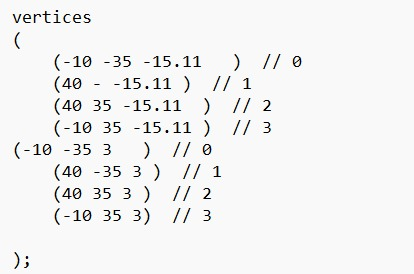
\includegraphics[width=\textwidth]{figures/ch8_domaine_70m.jpeg}
    \caption{Vue du domaine de calcul 3D sous OpenFOAM — longueur totale de 70\,m englobant la retenue amont, l'ouvrage (seuil Creager, coursier, cuillère) et la zone d'impact aval.}
    \label{fig:domaine_70m}
\end{figure}

Bien que la longueur totale de l'évacuateur soit de 70 m, les simulations de production ont été réalisées sur un domaine réduit de \textbf{20 m} dans la direction transversale. Ce choix se justifie par le caractère \textbf{homogène} de l'ouvrage : la géométrie (profil Creager, coursier, cuillère) est strictement identique en tout point de la largeur du barrage, de sorte que l'écoulement qui se développe sur une tranche de 20 m est en tous points représentatif de ce qui se produit sur l'ensemble des 70 m. Réduire le domaine à 20 m permet ainsi de diviser significativement le nombre de cellules du maillage et, par conséquent, le temps de calcul, sans introduire aucune approximation sur les résultats hydrauliques.

% SECTION : GÉNÉRATION DU MAILLAGE
\section{Génération du maillage}
\label{sec:generation_maillage}

\subsection{Initialisation du cas de simulation}
\label{subsec:initialisation_cas}

Avant de procéder à la génération du maillage, le cas OpenFOAM est initialisé en créant l'arborescence standard du répertoire de travail. La figure \ref{fig:dossier_initiation} présente la structure du dossier du cas, conforme à l'organisation décrite au chapitre \ref{chap:structure_cfd_openfoam} :

\begin{figure}[H]
    \centering
    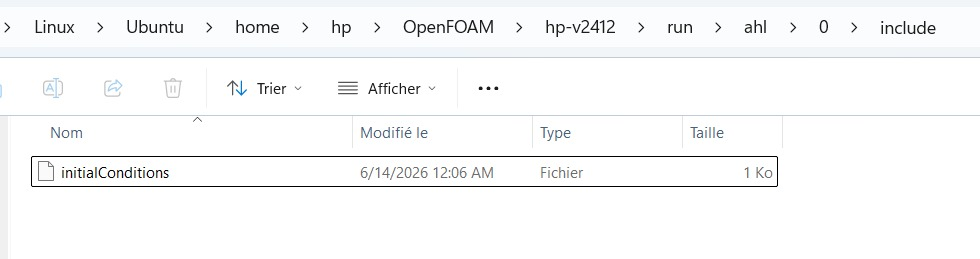
\includegraphics[width=0.70\textwidth]{figures/ch8_dossier_initiation.jpeg}
    \caption{Structure du dossier du cas OpenFOAM pour la simulation de l'évacuateur de crues — répertoires \texttt{0/}, \texttt{constant/} et \texttt{system/} avec leurs fichiers de configuration respectifs.}
    \label{fig:dossier_initiation}
\end{figure}

Le répertoire \texttt{0/} contient les fichiers décrivant les conditions initiales de chaque champ (\texttt{alpha.water}, \texttt{U}, \texttt{p\_rgh}, \texttt{k}, \texttt{omega}). La figure \ref{fig:condition_initiale} montre le contenu de ces fichiers d'initialisation :

\begin{figure}[H]
    \centering
    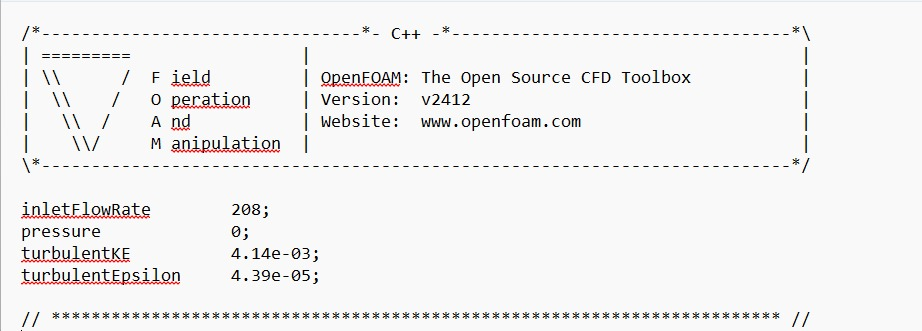
\includegraphics[width=\textwidth]{figures/ch8_condition_initiale.jpeg}
    \caption{Fichiers du répertoire \texttt{0/} du cas OpenFOAM — définition des conditions initiales des champs \texttt{alpha.water}, \texttt{U}, \texttt{p\_rgh} et des grandeurs de turbulence.}
    \label{fig:condition_initiale}
\end{figure}

Une fois les fichiers de conditions initiales en place, la commande \texttt{setFields} est exécutée pour initialiser les champs de manière cohérente avec la géométrie du domaine : le champ \texttt{alpha.water} est mis à 1 dans la zone du réservoir (eau) et à 0 dans la zone atmosphérique (air), en s'appuyant sur les régions de cellules définies dans \texttt{setFieldsDict}. La figure \ref{fig:setfields} illustre l'interface de cette commande :

\begin{figure}[H]
    \centering
    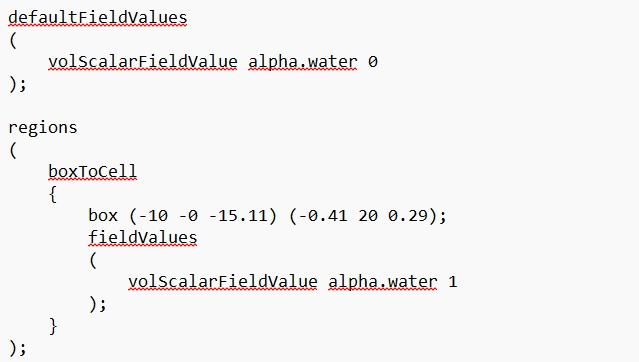
\includegraphics[width=\textwidth]{figures/ch8_setfields.jpeg}
    \caption{Exécution de la commande \texttt{setFields} — initialisation du champ \texttt{alpha.water} à 1 dans la zone de la retenue et à 0 dans la zone atmosphérique, conformément au fichier \texttt{system/setFieldsDict}.}
    \label{fig:setfields}
\end{figure}

Le profil de la surface libre initiale obtenu après l'exécution de \texttt{setFields}, visualisé sous ParaView, confirme que la répartition eau/air est correctement définie au démarrage de la simulation :

\begin{figure}[H]
    \centering
    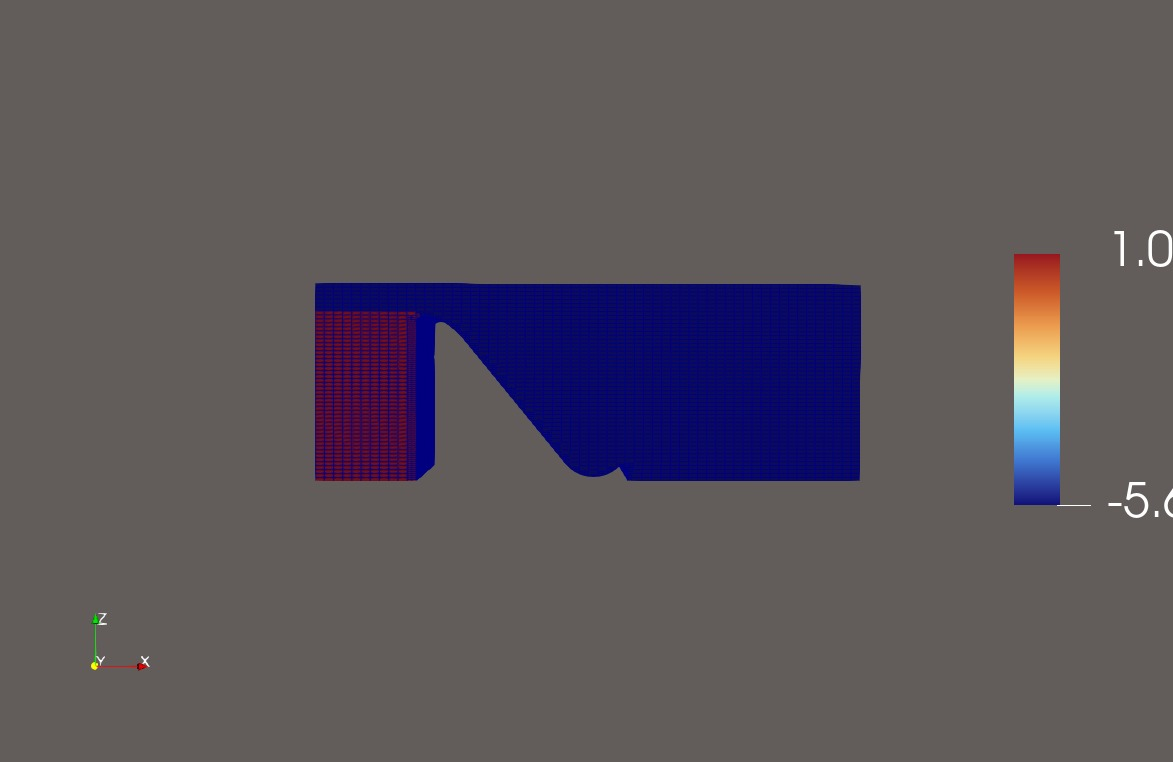
\includegraphics[width=\textwidth]{figures/ch8_profil_clair.jpeg}
    \caption{Profil de la surface libre initiale après \texttt{setFields} — visualisation du champ \texttt{alpha.water} (eau en bleu, air en blanc) à $t = 0$ dans ParaView ; le niveau d'eau dans la retenue correspond au niveau de la retenue normale.}
    \label{fig:profil_clair}
\end{figure}

\subsection{Maillage de base (blockMesh)}
\label{subsec:blockmesh}

La première étape de la génération du maillage consiste à définir, via l'utilitaire \texttt{blockMesh} et son fichier de configuration \texttt{blockMeshDict}, un maillage de fond hexaédrique englobant l'ensemble du domaine de calcul défini à la section \ref{sec:preparation_geometrie}. Ce maillage de base, relativement grossier, constitue le point de départ du raffinement effectué par \texttt{snappyHexMesh} \cite{greenshields2020openfoam, openfoam2022guide}.

Le maillage de fond obtenu après l'exécution de \texttt{blockMesh} est illustré par la figure suivante :

\begin{figure}[H]
    \centering
    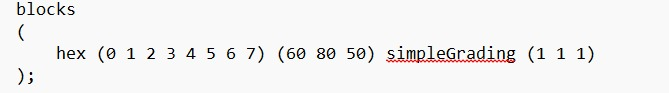
\includegraphics[width=\textwidth]{figures/ch8_maillage_grossier.jpeg}
    \caption{Vue d'ensemble du maillage de fond hexaédrique généré par \texttt{blockMesh} — maillage non raffiné couvrant l'intégralité du domaine de calcul (coupe verticale dans le plan médian de l'évacuateur).}
    \label{fig:maillage_global}
\end{figure}

\subsection{Raffinement et capture de la géométrie (snappyHexMesh)}
\label{subsec:snappyhexmesh}

L'utilitaire \texttt{snappyHexMesh} est ensuite utilisé pour adapter le maillage de fond aux surfaces STL importées (section \ref{sec:preparation_geometrie}), selon les trois étapes classiques \cite{greenshields2020openfoam} :
\begin{enumerate}
    \item \textbf{Castellation} : découpage des cellules du maillage de fond intersectant les surfaces STL ;
    \item \textbf{Snapping} : projection des points du maillage sur les surfaces STL pour reproduire fidèlement la géométrie de l'ouvrage (profil Creager, coursier, cuillère) ;
    \item \textbf{Ajout de couches limites (\textit{layers})} : insertion de couches de cellules fines au voisinage immédiat des parois solides, afin de mieux résoudre les gradients de vitesse dans la couche limite et d'atteindre une valeur de $y^+$ compatible avec les fonctions de paroi du modèle de turbulence retenu (section \ref{sec:conditions_limites}).
\end{enumerate}

Des zones de raffinement local (\texttt{refinementRegions} et \texttt{refinementSurfaces}) sont définies :
\begin{itemize}
    \item Au voisinage de l'\textbf{interface air-eau} (zone de battement du champ \texttt{alpha.water}), afin de limiter la diffusion numérique de l'interface et de capturer précisément la ligne d'eau le long du coursier ;
    \item Au voisinage du \textbf{seuil, du coursier et de la cuillère}, où les gradients de vitesse et de pression sont les plus marqués ;
    \item Le long de la \textbf{trajectoire théorique du jet} (section \ref{sec:distance_impact_jet}), pour assurer une résolution suffisante de la zone d'impact et de la fosse d'érosion (section \ref{sec:affouillement}).
\end{itemize}

Le fichier de configuration \texttt{snappyHexMeshDict} regroupe l'ensemble de ces paramètres de raffinement. La figure \ref{fig:snappyhexmeshdict} en présente un extrait :

\begin{figure}[H]
    \centering
    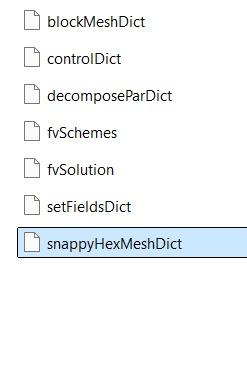
\includegraphics[height=0.55\textheight,keepaspectratio]{figures/ch8_snappyhexmeshdict.jpeg}
    \caption{Extrait du fichier \texttt{system/snappyHexMeshDict} — paramétrage des niveaux de raffinement par surface (\texttt{refinementSurfaces}) et par région (\texttt{refinementRegions}), ainsi que des paramètres de couches limites (\texttt{addLayersControls}).}
    \label{fig:snappyhexmeshdict}
\end{figure}

La qualité du maillage final est vérifiée à l'aide de l'utilitaire \texttt{checkMesh}, qui contrôle notamment la non-orthogonalité maximale, le \textit{skewness} et le rapport d'aspect des cellules \cite{knupp1993fundamentals}. Ces indicateurs doivent rester dans des plages compatibles avec la stabilité et la précision des schémas numériques du solveur \texttt{interFoam} (section \ref{sec:configuration_solveur}).

Le maillage raffiné obtenu après l'exécution de \texttt{snappyHexMesh} est présenté à la figure \ref{fig:maillage_detail} :

\begin{figure}[H]
    \centering
    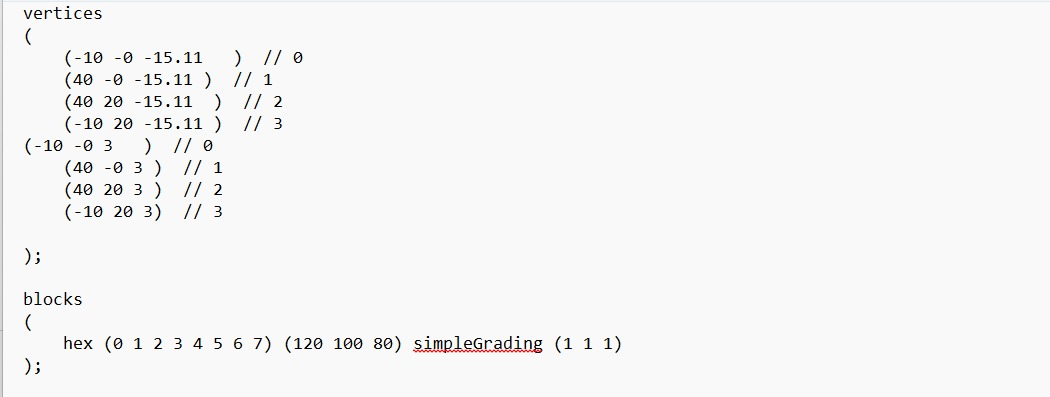
\includegraphics[width=\textwidth]{figures/ch8_maillage_raffine.jpeg}
    \caption{Vue rapprochée du maillage raffiné généré par \texttt{snappyHexMesh} au niveau du seuil Creager, du coursier et de la cuillère saut de ski — les couches de raffinement local et les couches limites sont clairement visibles au voisinage des parois solides.}
    \label{fig:maillage_detail}
\end{figure}

\subsection{Étude de sensibilité au maillage}
\label{subsec:sensibilite_maillage}

Afin de s'assurer que les résultats de la simulation sont indépendants de la résolution du maillage, une étude de sensibilité a été menée en comparant trois niveaux de raffinement (grossier, moyen, fin), construits en faisant varier le niveau de raffinement global et local de \texttt{snappyHexMesh} \cite{roache1998verification}. Pour chaque maillage, une grandeur de référence (par exemple la hauteur d'eau sur le coursier en une section donnée) est comparée entre les trois niveaux, afin de retenir le maillage offrant le meilleur compromis entre précision des résultats et coût de calcul.

Dans le cadre de cette étude, deux simulations ont été réalisées pour le débit millénal $Q_{1\,000} = 794{,}93$ m³/s :
\begin{itemize}
    \item \textbf{Simulation sur le domaine 70 m avec maillage non raffiné} : ce cas a d'abord été effectué pour visualiser l'écoulement sur la totalité de la structure. Le maillage utilisé est le maillage de fond grossier issu de \texttt{blockMesh} (figure \ref{fig:maillage_global}).
    \item \textbf{Simulation sur le domaine 20 m avec maillage raffiné} : ce cas constitue la simulation de référence. Le maillage est celui généré par \texttt{snappyHexMesh} avec raffinement local au niveau de l'ouvrage (figure \ref{fig:maillage_detail}).
\end{itemize}

La grandeur de comparaison est le champ \texttt{alpha.water} (fraction volumique d'eau), qui représente directement la position de la surface libre. Les profils \texttt{alpha.water} obtenus avec les deux configurations sont superposés : si les résultats concordent, la simulation sur 20 m avec maillage raffiné est validée et retenue pour l'ensemble de l'étude.


Les figures \ref{fig:alpha_70_grossier} et \ref{fig:alpha_20_raffine} présentent les champs \texttt{alpha.water} obtenus pour chacune des deux configurations, visualisés dans le plan médian longitudinal de l'évacuateur.

\begin{figure}[H]
    \centering
    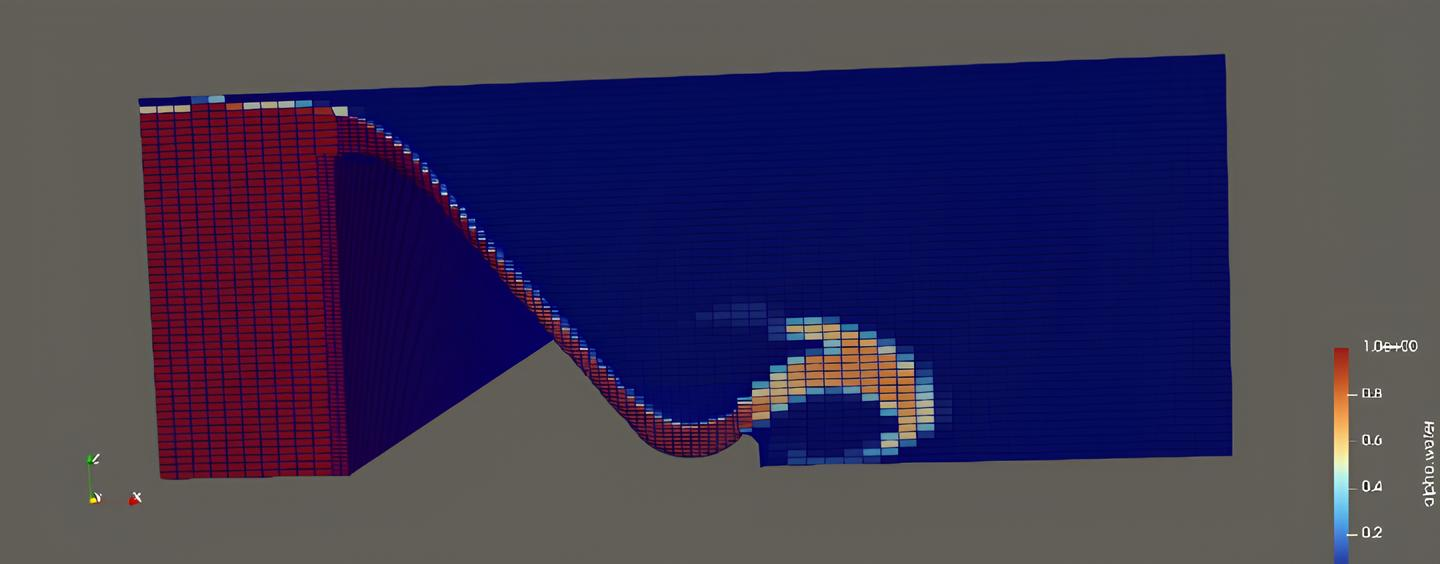
\includegraphics[width=\textwidth]{figures/ch8_alpha_70_grossier.jpeg}
    \caption{Champ \texttt{alpha.water} — domaine 70\,m avec maillage non raffiné (\texttt{blockMesh}), débit millénal $Q_{1\,000} = 794{,}93$ m³/s. La surface libre (interface eau/air) est visible mais sa définition reste approximative en raison de la faible résolution du maillage grossier.}
    \label{fig:alpha_70_grossier}
\end{figure}

\begin{figure}[H]
    \centering
    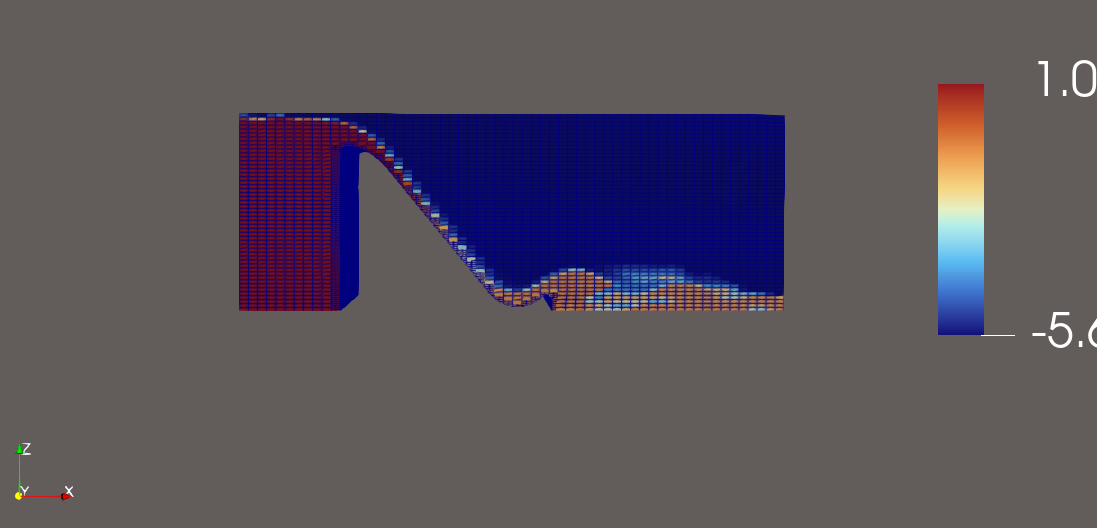
\includegraphics[width=\textwidth]{figures/ch8_alpha_20_raffine.png}
    \caption{Champ \texttt{alpha.water} — domaine 20\,m avec maillage raffiné (\texttt{snappyHexMesh}), débit millénal $Q_{1\,000} = 794{,}93$ m³/s. L'interface eau/air est nettement plus précise et la surface libre sur le coursier est bien capturée grâce au raffinement local.}
    \label{fig:alpha_20_raffine}
\end{figure}

La comparaison des deux champs \texttt{alpha.water} montre que les profils de la surface libre obtenus avec les deux configurations sont \textbf{en accord} : la position de l'interface eau/air, la hauteur d'eau sur le seuil et le long du coursier, ainsi que la trajectoire du jet en aval de la cuillère sont cohérents entre les deux simulations. La simulation sur le domaine réduit de 20 m avec maillage raffiné reproduit donc fidèlement les résultats du domaine complet de 70 m, tout en offrant une résolution spatiale nettement supérieure au niveau de l'ouvrage.

\bigskip
Afin de renforcer cette validation, le \textbf{champ de vitesse U} a également été comparé entre les deux configurations. La distribution spatiale des vitesses constitue en effet un indicateur sensible de la qualité du maillage : un maillage insuffisamment raffiné tend à lisser les gradients de vitesse, à sous-estimer les vitesses maximales au voisinage des parois et à mal reproduire la structure de l'écoulement dans les zones de forte courbure (seuil, cuillère).

\begin{figure}[H]
    \centering
    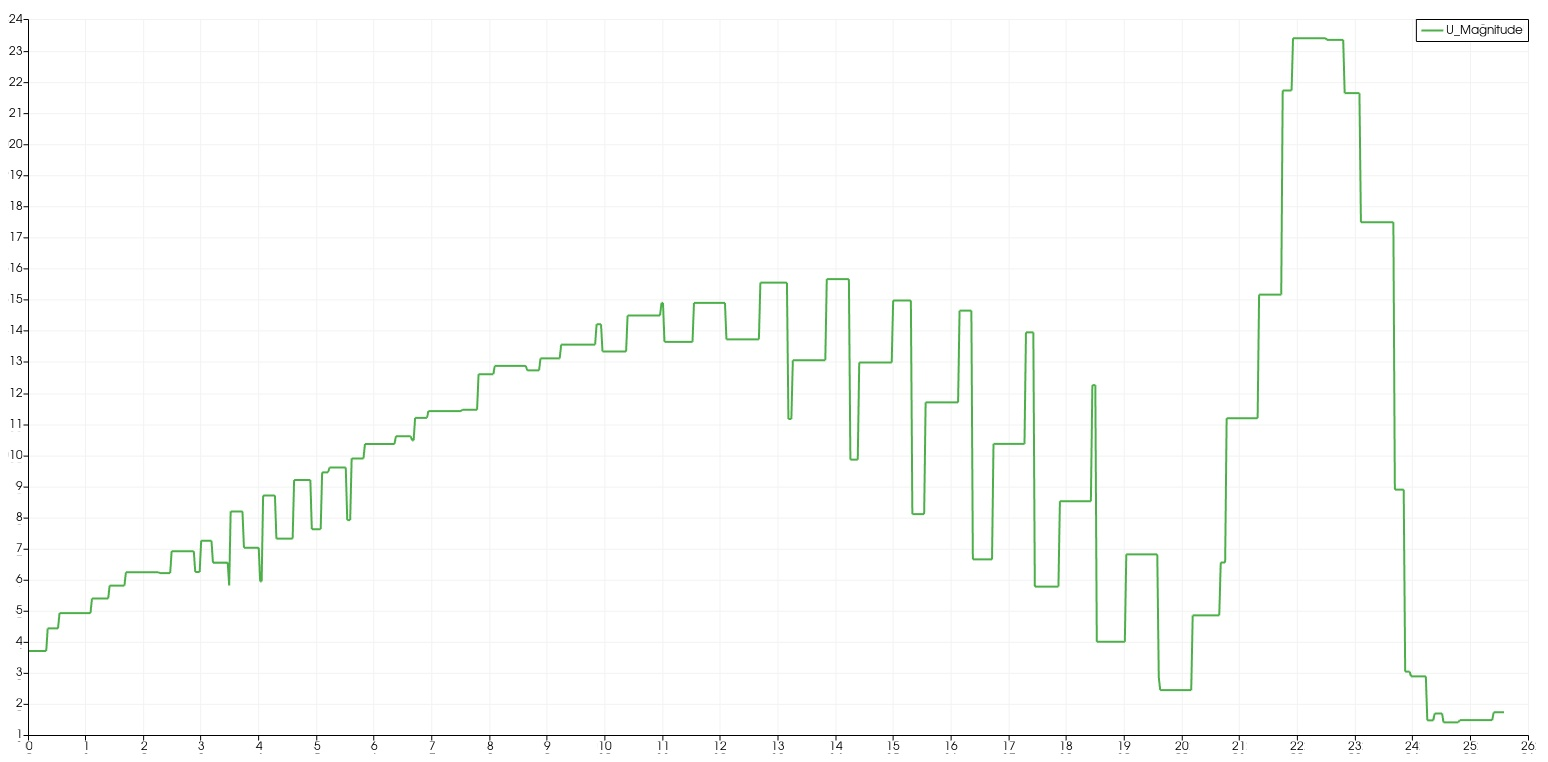
\includegraphics[width=\textwidth]{figures/ch8_U_70_grossier.jpeg}
    \caption{Champ de vitesse $\|\mathbf{U}\|$ (m/s) — domaine 70\,m avec maillage non raffiné (\texttt{blockMesh}), débit millénal $Q_{1\,000} = 794{,}93$ m³/s. Les gradients de vitesse sont peu résolus et la distribution apparaît homogène par excès de diffusion numérique due à la grande taille des cellules.}
    \label{fig:U_70_grossier}
\end{figure}

\begin{figure}[H]
    \centering
    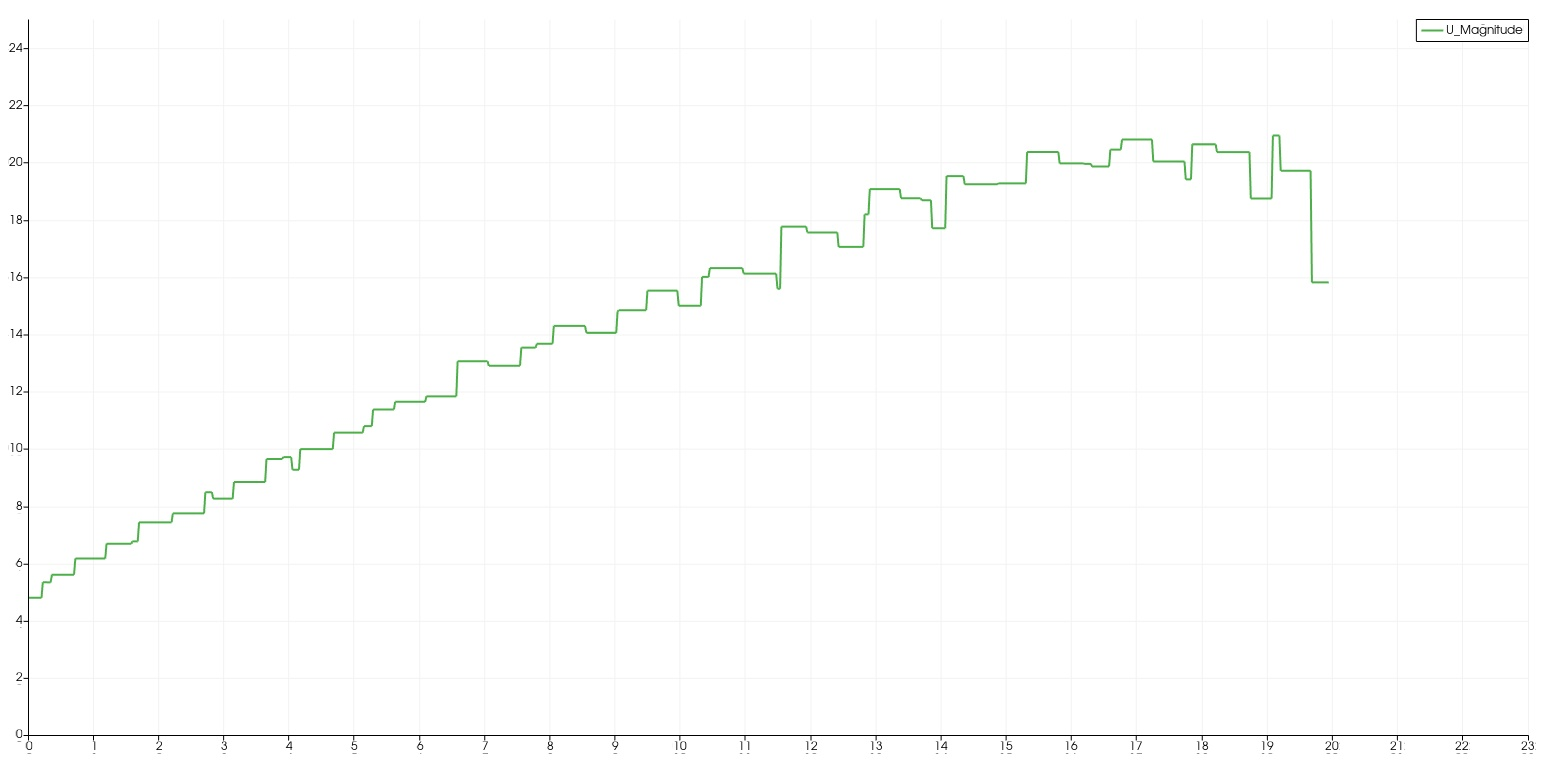
\includegraphics[width=\textwidth]{figures/ch8_U_20_raffine.jpeg}
    \caption{Champ de vitesse $\|\mathbf{U}\|$ (m/s) — domaine 20\,m avec maillage raffiné (\texttt{snappyHexMesh}), débit millénal $Q_{1\,000} = 794{,}93$ m³/s. Les gradients de vitesse sont nettement mieux résolus : l'accélération de l'écoulement sur le seuil Creager, les vitesses élevées sur le coursier et la distribution du jet en aval de la cuillère sont clairement visibles.}
    \label{fig:U_20_raffine}
\end{figure}

La comparaison des deux champs de vitesse met en évidence l'apport du raffinement du maillage :
\begin{itemize}
    \item Sur le \textbf{maillage grossier} (70 m), les gradients de vitesse sont diffus et les vitesses maximales sont sous-estimées ; la structure de l'écoulement au niveau du seuil et de la cuillère est imprécise.
    \item Sur le \textbf{maillage raffiné} (20 m), les vitesses sont bien résolues, les zones d'accélération et de décélération sont nettement distinguées, et la distribution transversale de l'écoulement est cohérente avec les résultats théoriques du chapitre \ref{chap:dimensionnement_theorique}.
\end{itemize}

L'accord global entre les champs \texttt{alpha.water} et les champs de vitesse des deux configurations confirme la \textbf{convergence en maillage} de la solution : le maillage raffiné sur 20 m capture correctement la physique de l'écoulement et constitue un choix pertinent pour l'ensemble des simulations de production présentées au chapitre \ref{chap:resultats_simulation}.

Le maillage retenu pour l'ensemble des simulations présentées dans ce rapport est celui offrant un écart négligeable sur la grandeur de référence par rapport au maillage le plus fin, pour un coût de calcul maîtrisé.

\subsection{Visualisation du maillage sous ParaView}
\label{subsec:visualisation_paraview}

La géométrie maillée est chargée sous \textbf{ParaView} en ouvrant le fichier \texttt{ahl.foam} généré dans le répertoire du cas. Cette opération permet de vérifier visuellement la cohérence du maillage avec la géométrie STL importée, et de contrôler la qualité du raffinement au voisinage de l'ouvrage.

\begin{figure}[H]
    \centering
    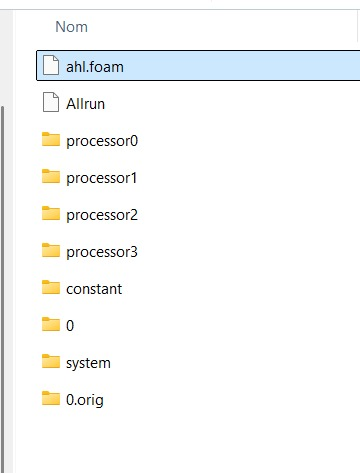
\includegraphics[height=0.55\textheight,keepaspectratio]{figures/ch8_paraview_ahl.jpeg}
    \caption{Ouverture du cas OpenFOAM dans ParaView via le fichier \texttt{ahl.foam} — la géométrie complète de l'évacuateur de crues (profil Creager, coursier, cuillère) apparaît correctement chargée avec son maillage raffiné.}
    \label{fig:paraview_ahl}
\end{figure}

\begin{figure}[H]
    \centering
    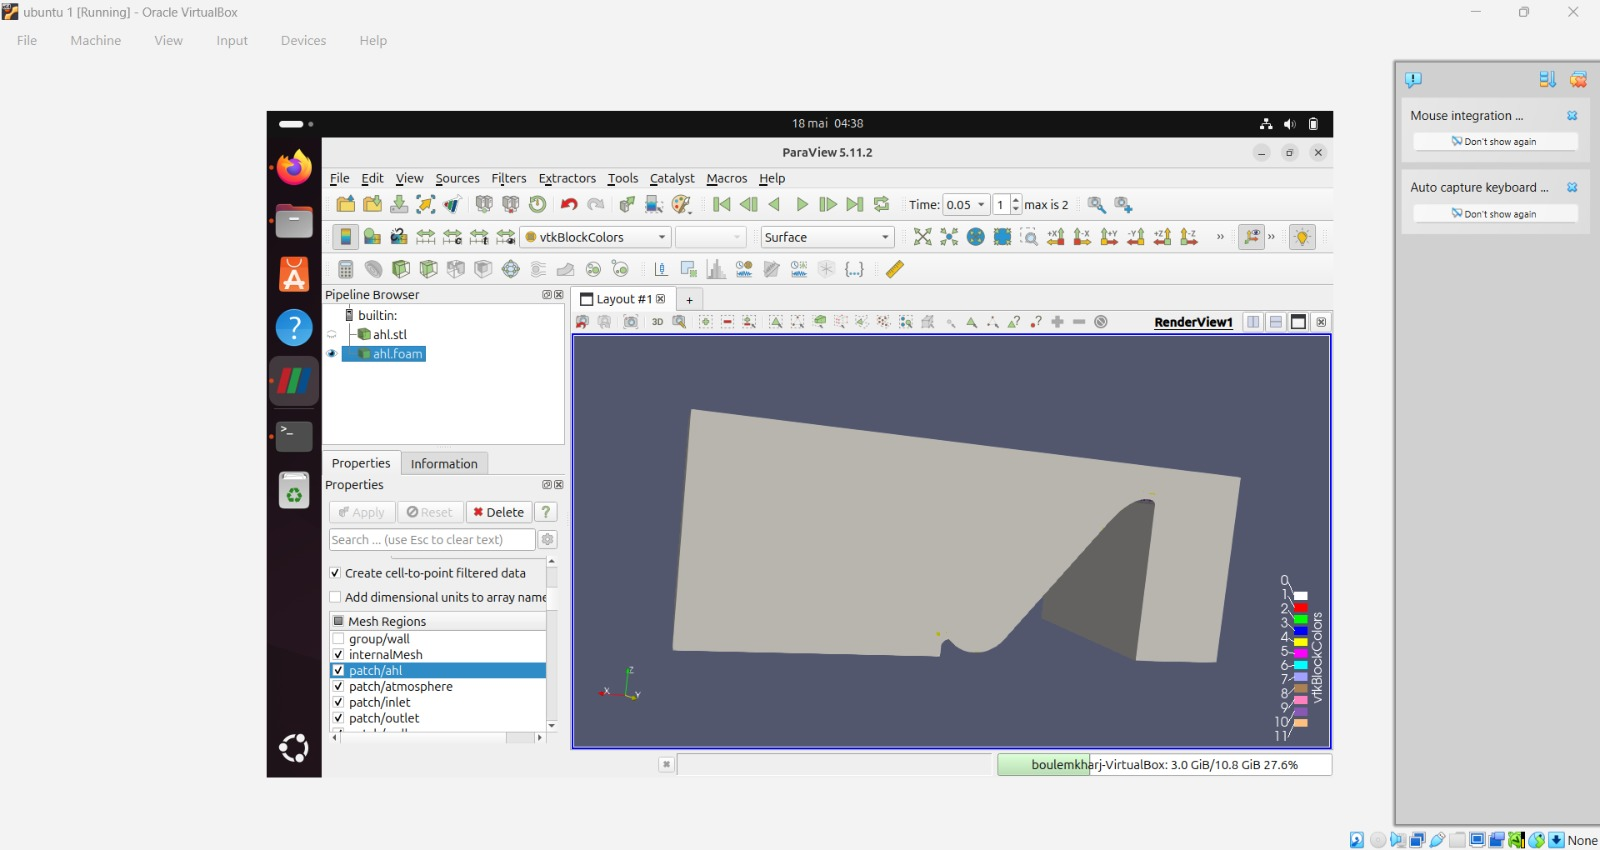
\includegraphics[width=\textwidth]{figures/ch8_paraview1.jpeg}
    \caption{Visualisation du maillage de l'évacuateur de crues sous ParaView (vue 1) — vue d'ensemble du domaine de calcul montrant la répartition des cellules du maillage et les zones de raffinement local.}
    \label{fig:paraview1}
\end{figure}


% SECTION : CONDITIONS INITIALES ET AUX LIMITES
\section{Conditions initiales et conditions aux limites}
\label{sec:conditions_limites}

\subsection{Conditions initiales}
\label{subsec:conditions_initiales}

À l'instant initial ($t=0$), le domaine de calcul est initialisé à l'aide de l'utilitaire \texttt{setFields}, selon les principes suivants :
\begin{itemize}
    \item Le champ \texttt{alpha.water} est initialisé à 1 dans la portion du domaine située sous le niveau d'eau correspondant au débit simulé (niveau de retenue normale $Z = 600{,}00$ NGM majoré de la charge $H$ du tableau \ref{tab:loi_debit_charge}), et à 0 ailleurs (zone atmosphérique et coursier initialement sec) ;
    \item Le champ de pression \texttt{p\_rgh} est initialisé de manière hydrostatique, cohérent avec la répartition initiale du champ \texttt{alpha.water} ;
    \item Le champ de vitesse \texttt{U} est initialisé à $\mathbf{0}$ (eau initialement au repos), l'écoulement se développant progressivement sous l'effet du déversement sur le seuil ;
    \item Les champs de turbulence \texttt{k} et \texttt{omega} sont initialisés à des valeurs uniformes faibles, estimées à partir d'une intensité turbulente caractéristique et d'une longueur de mélange représentative de la géométrie de l'écoulement \cite{menter1994two}.
\end{itemize}

\subsection{Conditions aux limites}
\label{subsec:conditions_aux_limites}

Les conditions aux limites sont définies pour chaque frontière (\textit{patch}) du domaine de calcul, en cohérence avec les types de conditions présentés au chapitre \ref{chap:structure_cfd_openfoam} (tableau \ref{tab:boundary_conditions}). Le tableau \ref{tab:cl_ahl_souss} synthétise les conditions retenues pour les principaux champs (\texttt{alpha.water}, \texttt{U}, \texttt{p\_rgh}, \texttt{k}, \texttt{omega}) sur chacune des frontières du domaine.

\begin{table}[H]
    \centering
    \caption{Conditions aux limites retenues pour le cas Ahl Souss}
    \label{tab:cl_ahl_souss}
    \resizebox{\textwidth}{!}{%
    \begin{tabular}{|l|c|c|c|c|c|}
        \hline
        \textbf{Frontière} & \textbf{\texttt{alpha.water}} & \textbf{\texttt{U}} & \textbf{\texttt{p\_rgh}} & \textbf{\texttt{k} / \texttt{omega}} & \textbf{Remarque} \\
        \hline
        Amont (réservoir) & \texttt{fixedValue} & \texttt{pressureInletOutletVelocity} & \texttt{totalPressure} & \texttt{fixedValue} & Niveau d'eau imposé selon $Q$ \\
        \hline
        Aval (sortie) & \texttt{inletOutlet} & \texttt{pressureInletOutletVelocity} & \texttt{totalPressure} & \texttt{inletOutlet} & Sortie libre \\
        \hline
        Atmosphère (haut) & \texttt{inletOutlet} & \texttt{pressureInletOutletVelocity} & \texttt{totalPressure} & \texttt{inletOutlet} & Pression atmosphérique \\
        \hline
        Parois (fond, ouvrage) & \texttt{zeroGradient} & \texttt{noSlip} & \texttt{fixedFluxPressure} & \texttt{kqRWallFunction} / \texttt{omegaWallFunction} & Fonctions de paroi, $k-\omega$ SST \\
        \hline
        Plans latéraux & \texttt{zeroGradient} & \texttt{slip} ou \texttt{symmetry} & \texttt{zeroGradient} / \texttt{symmetry} & \texttt{symmetry} & Selon configuration retenue \\
        \hline
    \end{tabular}}
\end{table}

Le modèle de turbulence retenu est le modèle $k-\omega$ SST de Menter \cite{menter1994two}, déjà présenté au chapitre \ref{chap:turbulence} (section \ref{subsec:modele_k_omega_sst}), qui offre un bon compromis entre robustesse et précision pour les écoulements à surface libre comportant à la fois des zones de proche paroi et des zones de cisaillement libre (jet, surface libre) \cite{moukalled2016finite}.

% SECTION : CONFIGURATION DU SOLVEUR INTERFOAM
\section{Configuration du solveur interFoam}
\label{sec:configuration_solveur}

\subsection{Schémas de discrétisation (fvSchemes)}
\label{subsec:fvschemes}

Le fichier \texttt{fvSchemes} définit les schémas numériques utilisés pour discrétiser les différents termes des équations résolues par \texttt{interFoam} \cite{rusche2002computational} :
\begin{itemize}
    \item \textbf{Schéma temporel (\texttt{ddtSchemes})} : schéma \texttt{Euler}, implicite du premier ordre, adapté au pas de temps variable utilisé en régime transitoire ;
    \item \textbf{Schémas de gradient (\texttt{gradSchemes})} : schéma \texttt{Gauss linear}, du second ordre ;
    \item \textbf{Schémas de divergence (\texttt{divSchemes})} : un schéma de type \texttt{vanLeer}, borné et peu diffusif, est utilisé pour l'advection du champ \texttt{alpha.water} (méthode MULES) afin de préserver la netteté de l'interface air-eau ; des schémas de type \texttt{linearUpwind} ou \texttt{limitedLinear} sont utilisés pour le terme convectif de \texttt{U} et pour les équations de turbulence ($k$, $\omega$), afin de garantir la stabilité du calcul ;
    \item \textbf{Schémas laplaciens (\texttt{laplacianSchemes})} : schéma \texttt{Gauss linear corrected}, avec correction de non-orthogonalité ;
    \item \textbf{Schémas d'interpolation} : interpolation linéaire entre centres de cellules et faces.
\end{itemize}

\subsection{Paramètres de résolution (fvSolution) et algorithme PIMPLE}
\label{subsec:fvsolution}

Le fichier \texttt{fvSolution} définit les solveurs linéaires et leurs critères de convergence pour chaque champ, ainsi que les paramètres de l'algorithme de couplage pression-vitesse \cite{holzmann2017mathematics} :
\begin{itemize}
    \item Le champ \texttt{alpha.water} est résolu par la méthode \textbf{MULES} (\textit{Multidimensional Universal Limiter with Explicit Solution}), avec un nombre de sous-cycles (\texttt{nAlphaSubCycles}) et un coefficient de compression d'interface (\texttt{cAlpha}) permettant de limiter la diffusion numérique de l'interface air-eau ;
    \item Le champ de pression \texttt{p\_rgh} est résolu par un solveur de type \texttt{GAMG} (\textit{Geometric-Algebraic Multi-Grid}) ou \texttt{PCG} avec préconditionneur \texttt{DIC} ;
    \item Les champs \texttt{U}, \texttt{k} et \texttt{omega} sont résolus par un solveur de type \texttt{smoothSolver} ou \texttt{PBiCG} avec préconditionneur \texttt{DILU} ;
    \item L'algorithme \textbf{PIMPLE} (chapitre \ref{chap:structure_cfd_openfoam}, section \ref{subsec:pimple}) est configuré avec un nombre de correcteurs externes (\texttt{nOuterCorrectors}), un nombre de correcteurs de pression (\texttt{nCorrectors}) et un nombre de correcteurs de non-orthogonalité (\texttt{nNonOrthogonalCorrectors}) adaptés à la qualité du maillage (section \ref{subsec:sensibilite_maillage}) ;
    \item Des facteurs de sous-relaxation sont appliqués sur la pression et la vitesse au sein des itérations externes, afin de stabiliser la convergence à chaque pas de temps.
\end{itemize}


% SECTION : LANCEMENT DES SIMULATIONS ET CONVERGENCE
\section{Lancement des simulations et suivi de la convergence}
\label{sec:lancement_simulations}

\subsection{Campagne de simulations}
\label{subsec:campagne_simulations}

Conformément aux objectifs de l'étude, une simulation a été réalisée pour chacun des trois débits laminés du tableau \ref{tab:debits_lamines} (périodes de retour 10, 100 et 1\,000 ans), avec un maillage et une configuration de solveur identiques (sections \ref{sec:generation_maillage} et \ref{sec:configuration_solveur}), seule la condition à la limite amont (niveau d'eau / débit imposé) variant d'une simulation à l'autre. Un scénario complémentaire, correspondant à une surélévation hypothétique du plan d'eau de 1 m, est traité séparément à titre de supplément (chapitre \ref{chap:resultats_simulation}, section \ref{sec:supplement_surelevation}).

Les calculs ont été exécutés en parallèle à l'aide de la décomposition de domaine (\texttt{decomposePar}), selon une méthode de décomposition de type \textit{scotch}, répartissant le maillage sur plusieurs cœurs de calcul afin de réduire le temps de restitution.

La figure \ref{fig:decomposePar} illustre la configuration du fichier \texttt{decomposeParDict} utilisé pour la décomposition du domaine, et la figure \ref{fig:decomposePar_result} montre les répertoires générés après l'exécution de \texttt{decomposePar} :

\begin{figure}[H]
    \centering
    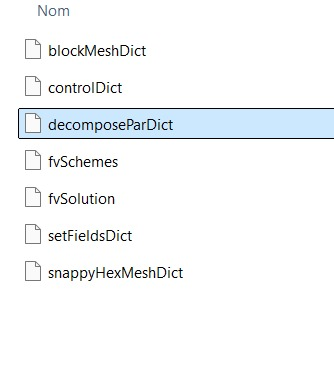
\includegraphics[width=\textwidth]{figures/ch8_decomposePar.jpeg}
    \caption{Configuration de la décomposition de domaine dans le fichier \texttt{system/decomposeParDict} — méthode \textit{scotch} avec répartition automatique du maillage entre les processeurs.}
    \label{fig:decomposePar}
\end{figure}

\begin{figure}[H]
    \centering
    
\includegraphics[width=\textwidth]{figures/ch8_decomposePar_result.jpeg}
    \caption{Répertoires créés par la commande \texttt{decomposePar} — chaque sous-répertoire \texttt{processor\textit{N}/} contient la portion du maillage et des champs attribuée au processeur \textit{N} pour le calcul parallèle.}
    \label{fig:decomposePar_result}
\end{figure}

\subsection{Suivi de la convergence}
\label{subsec:suivi_convergence}

La convergence et la stabilité de chaque simulation sont contrôlées tout au long du calcul à l'aide des indicateurs suivants :
\begin{itemize}
    \item Les \textbf{résidus} des champs \texttt{p\_rgh}, \texttt{Ux}, \texttt{Uy} et \texttt{Uz}, dont la décroissance traduit la convergence de la résolution à chaque pas de temps ;
    \item Le \textbf{nombre de Courant} (\texttt{Courant Number}), global et maximal, qui doit rester compatible avec les bornes \texttt{maxCo} et \texttt{maxAlphaCo} définies dans le fichier \texttt{controlDict} ;
    \item Les \textbf{erreurs de conservation de la masse} (\textit{continuity errors}), rapportées par \texttt{interFoam} à chaque pas de temps, qui doivent rester négligeables ;
    \item L'évolution temporelle de grandeurs physiques en des points de contrôle (sondes), telles que la hauteur d'eau ou la vitesse en une section donnée du coursier, dont la stabilisation traduit l'atteinte d'un régime quasi-permanent.
\end{itemize}


% ============================================================
%  CHAPITRE 9 : Résultats de la simulation et interprétation
% ============================================================
\chapter{Résultats de la simulation et interprétation}
\label{chap:resultats_simulation}

\section{Introduction}
\label{sec:intro_resultats}

Ce chapitre présente et analyse les résultats des simulations numériques OpenFOAM réalisées pour les trois débits laminés retenus : $Q_{10} = 160{,}74$ m³/s, $Q_{100} = 507{,}54$ m³/s et $Q_{1\,000} = 794{,}93$ m³/s. Pour chaque débit, les résultats sont présentés dans l'ordre suivant :
\begin{enumerate}
    \item \textbf{Champ de vitesse} : profil de la vitesse le long de l'évacuateur et graphe de l'évolution des valeurs exactes ;
    \item \textbf{Champ de pression} : profil de la pression le long de l'évacuateur et graphe des valeurs exactes ;
    \item \textbf{Hauteur d'eau} : visualisation de la lame d'eau aux trois points caractéristiques de l'ouvrage (seuil, coursier, cuillère) ;
    \item \textbf{Jet et point d'impact} : trajectoire du jet en aval de la cuillère et coordonnées du point d'impact.
\end{enumerate}

Toutes les visualisations sont réalisées sous ParaView \cite{ayachit2015paraview} à partir des champs \texttt{U}, \texttt{p\_rgh} et \texttt{alpha.water} extraits en régime quasi-permanent.

% ============================================================
%  SECTION 9.1 : Q10
% ============================================================
\section{Résultats pour le débit décennal $Q_{10} = 160{,}74$ m³/s}
\label{sec:resultats_q10}

\subsection{Champ de vitesse}
\label{subsec:q10_vitesse}

La figure \ref{fig:q10_U_profil} présente le profil de la vitesse $\|\mathbf{U}\|$ le long de l'évacuateur de crues dans le plan médian longitudinal, pour le débit décennal $Q_{10}$.

\begin{figure}[H]
    \centering
    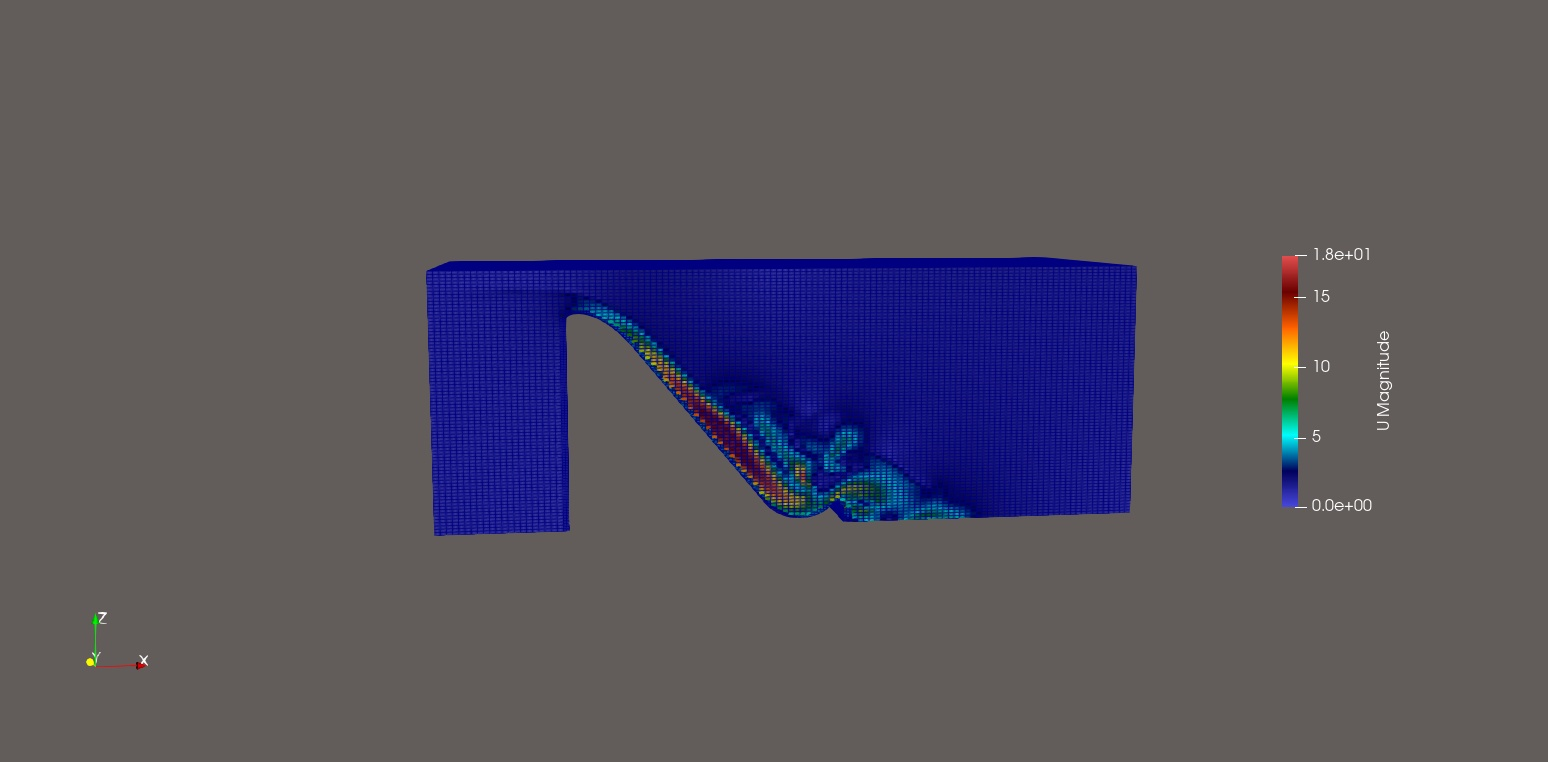
\includegraphics[width=\textwidth]{figures/ch9_q10_U_profil.jpeg}
    \caption{Profil du champ de vitesse $\|\mathbf{U}\|$ (m/s) le long de l'évacuateur de crues — débit décennal $Q_{10} = 160{,}74$ m³/s. L'écoulement s'accélère progressivement depuis la retenue jusqu'à la cuillère, où la vitesse atteint son maximum.}
    \label{fig:q10_U_profil}
\end{figure}

Le profil de vitesse montre une accélération progressive de l'écoulement depuis la zone de retenue (vitesses quasi nulles) jusqu'à la crête du seuil Creager, puis le long du coursier où l'écoulement devient nettement torrentiel. Les vitesses maximales sont atteintes à la sortie de la cuillère saut de ski. Le gradient de vitesse au voisinage des parois traduit bien le développement de la couche limite turbulente, correctement représenté par le modèle $k$-$\omega$ SST.

La figure \ref{fig:q10_U_graphe} présente l'évolution quantitative de la vitesse le long de l'axe longitudinal de l'évacuateur.

\begin{figure}[H]
    \centering
    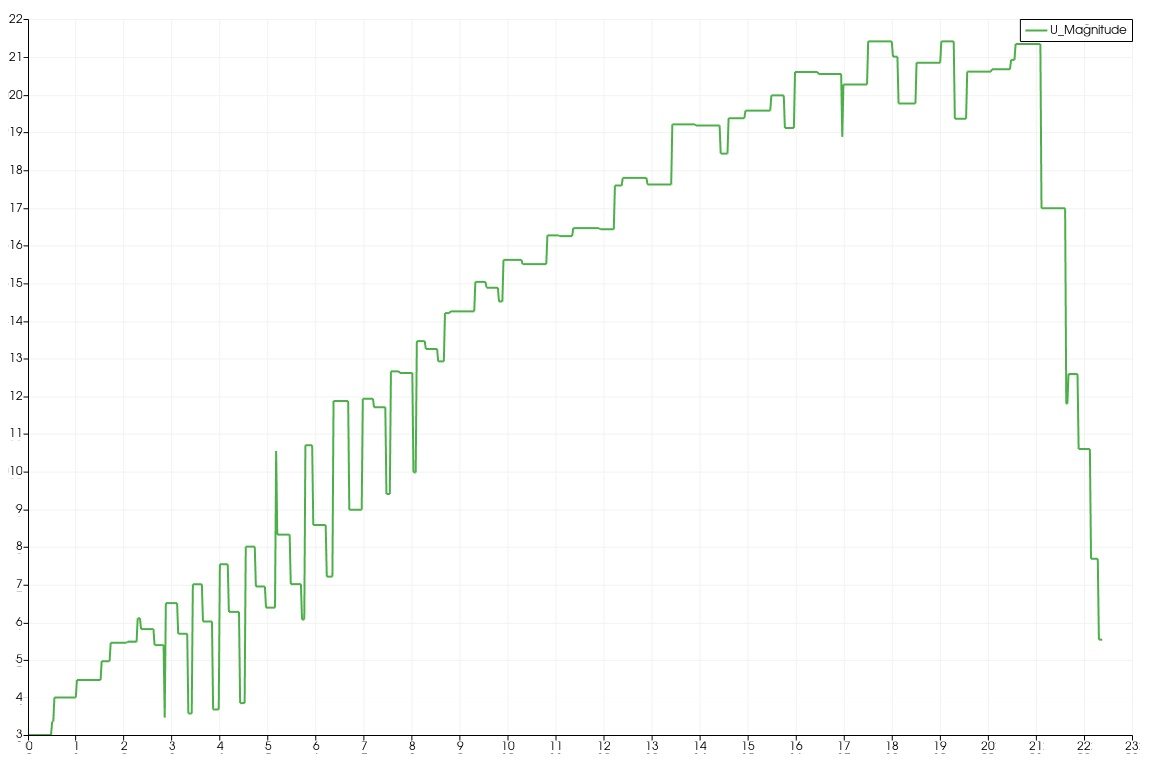
\includegraphics[width=\textwidth]{figures/ch9_q10_U_graphe.jpeg}
    \caption{Évolution de la vitesse $\|\mathbf{U}\|$ (m/s) le long de l'axe longitudinal de l'évacuateur — débit décennal $Q_{10} = 160{,}74$ m³/s. Les coordonnées curvilignes permettent de localiser précisément les zones d'accélération sur le seuil et le coursier.}
    \label{fig:q10_U_graphe}
\end{figure}

Le graphe confirme la montée monotone de la vitesse le long du coursier, caractéristique d'un écoulement supercritique en canal à forte pente. Les valeurs numériques obtenues sont cohérentes avec les résultats théoriques de la méthode des pas du chapitre \ref{chap:dimensionnement_theorique}.

\subsection{Champ de pression}
\label{subsec:q10_pression}

La figure \ref{fig:q10_P_profil} présente la distribution de la pression $p$ le long de l'évacuateur pour le débit décennal.

\begin{figure}[H]
    \centering
    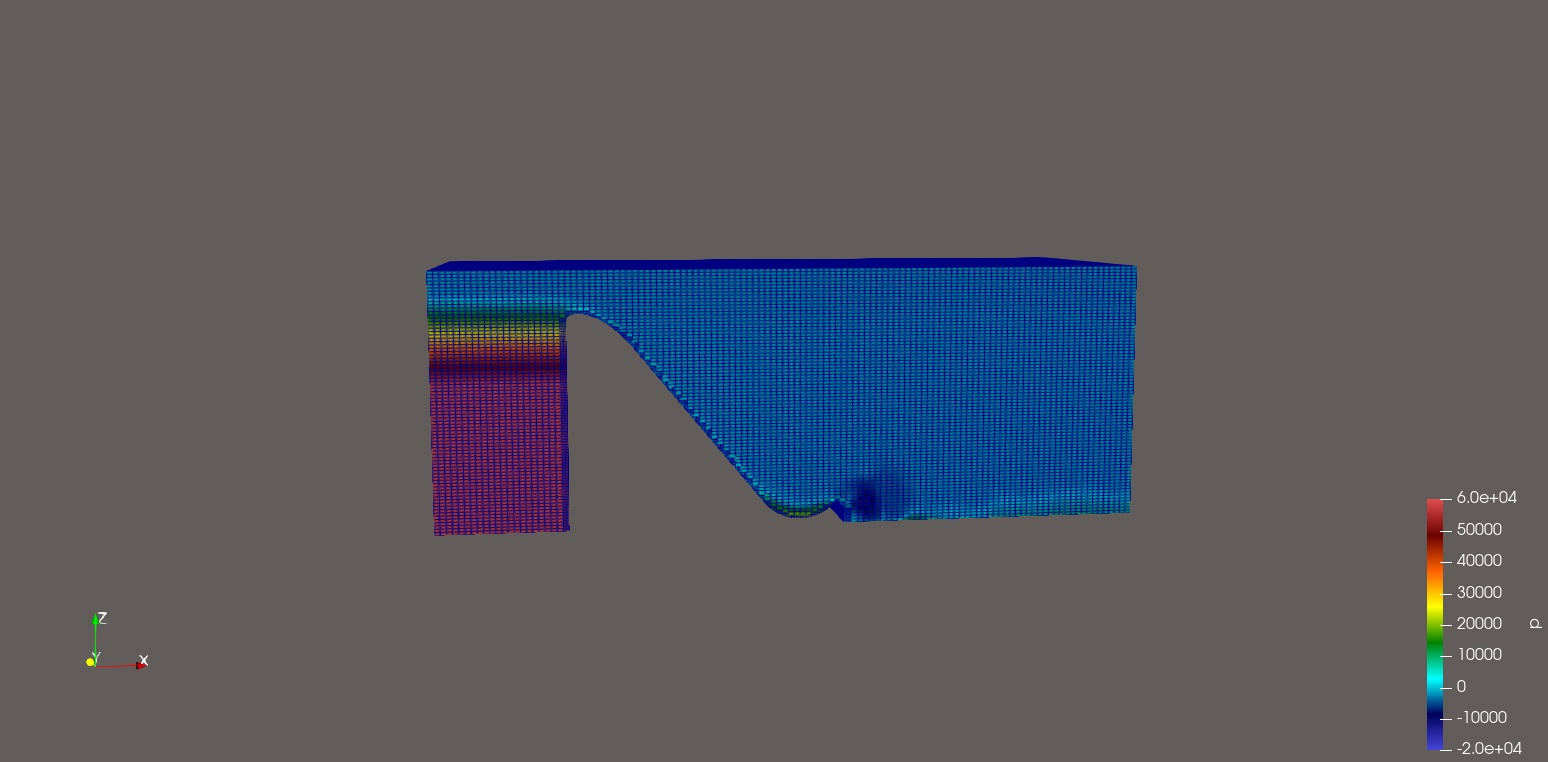
\includegraphics[width=\textwidth]{figures/ch9_q10_P_profil.jpeg}
    \caption{Profil du champ de pression $p$ (Pa) le long de l'évacuateur de crues — débit décennal $Q_{10} = 160{,}74$ m³/s. La pression est maximale dans la retenue amont (hydrostatique) et décroît le long du coursier ; une surpression locale est visible au niveau de la cuillère saut de ski.}
    \label{fig:q10_P_profil}
\end{figure}

Le profil de pression est dominé par la distribution hydrostatique dans la retenue amont. Le long du coursier, la pression diminue conformément à l'augmentation de vitesse (conservation de l'énergie). La courbure convexe de la cuillère saut de ski génère une surpression locale sur le radier, due à l'effet centrifuge de la déviation du jet — phénomène attendu et compatible avec la géométrie dimensionnée à la section \ref{sec:geometrie_cuillere}.

\begin{figure}[H]
    \centering
    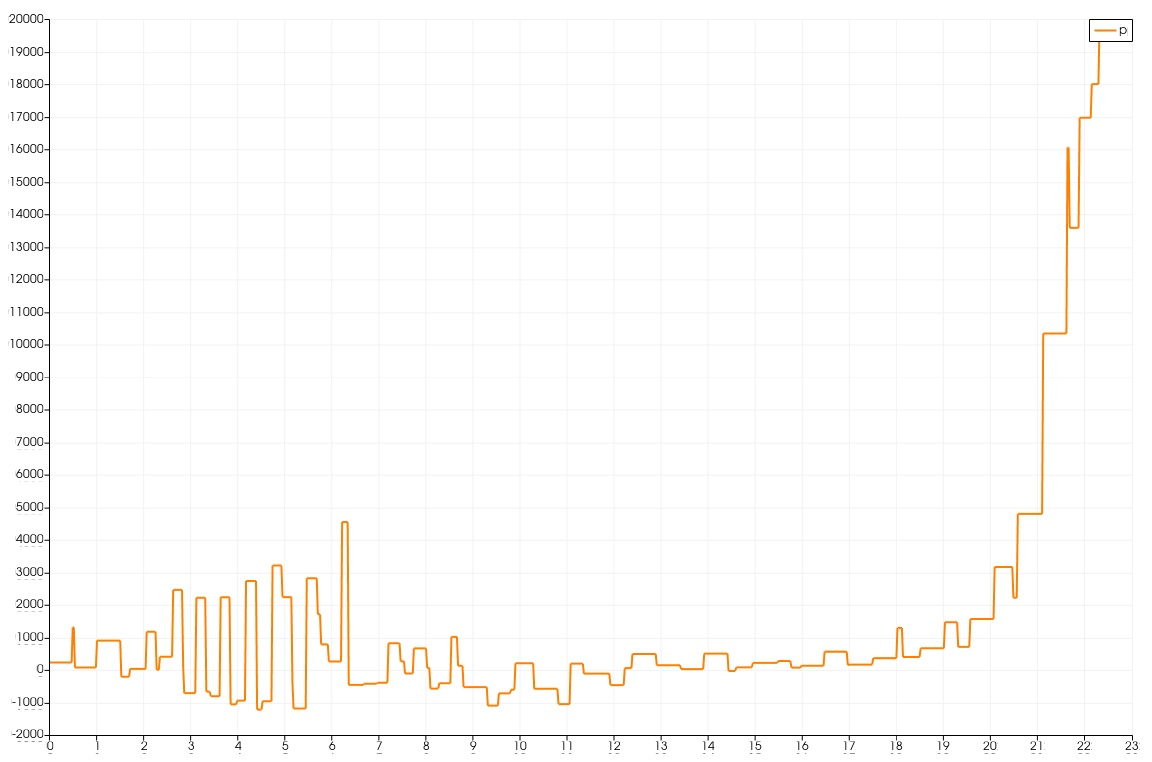
\includegraphics[width=\textwidth]{figures/ch9_q10_P_graphe.jpeg}
    \caption{Évolution de la pression $p$ (Pa) le long de l'axe longitudinal de l'évacuateur — débit décennal $Q_{10} = 160{,}74$ m³/s. La décroissance de pression le long du coursier et la surpression à la cuillère sont clairement identifiables.}
    \label{fig:q10_P_graphe}
\end{figure}

Le graphe de pression confirme les tendances observées sur le profil : la pression chute fortement à la crête du seuil (passage du régime fluvial au régime critique) puis continue de décroître sur le coursier torrentiel, avant d'augmenter légèrement à la cuillère sous l'effet de la courbure.

\subsection{Hauteur d'eau aux points caractéristiques}
\label{subsec:q10_hauteur}

Les figures suivantes présentent la hauteur d'eau aux trois points caractéristiques de l'ouvrage : le seuil, le coursier et la cuillère.

\begin{figure}[H]
    \centering
    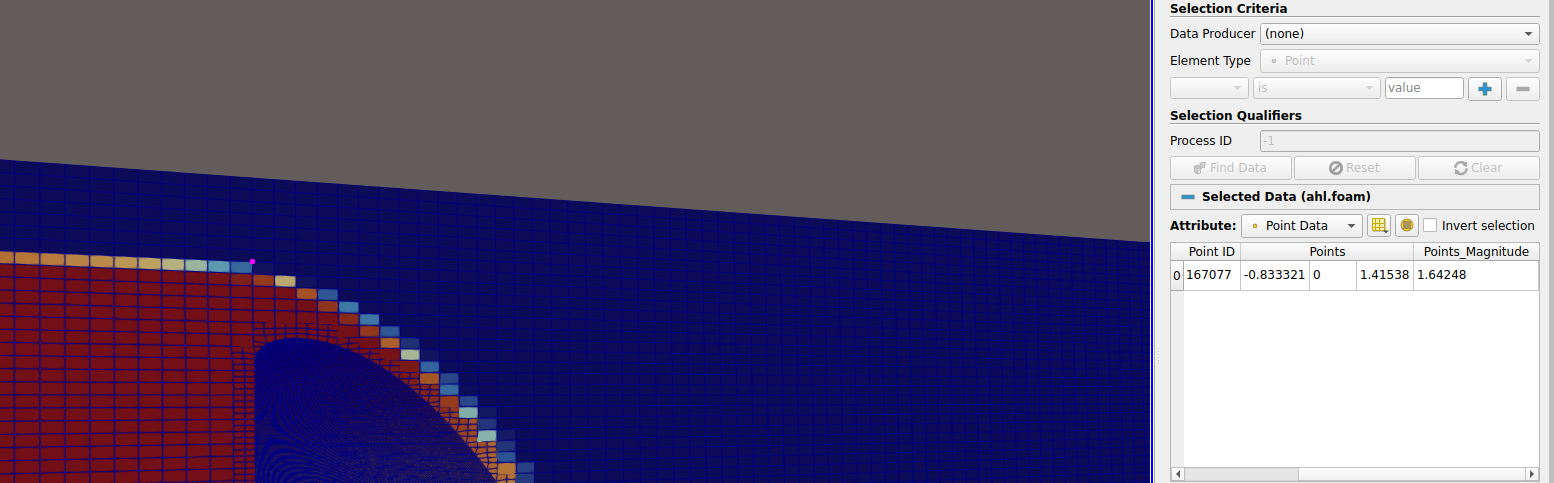
\includegraphics[width=\textwidth]{figures/ch9_q10_h_seuil.png}
    \caption{Hauteur d'eau au seuil Creager — débit décennal $Q_{10} = 160{,}74$ m³/s. La charge simulée sur le seuil est $H_d \approx 1{,}44$ m, lue sur le tableau de données ParaView (coordonnée verticale du point de surface libre sélectionné). Cette valeur correspond à la charge de déversement du seuil Creager (section \ref{sec:loi_debit_charge}).}
    \label{fig:q10_h_seuil}
\end{figure}

\begin{figure}[H]
    \centering
    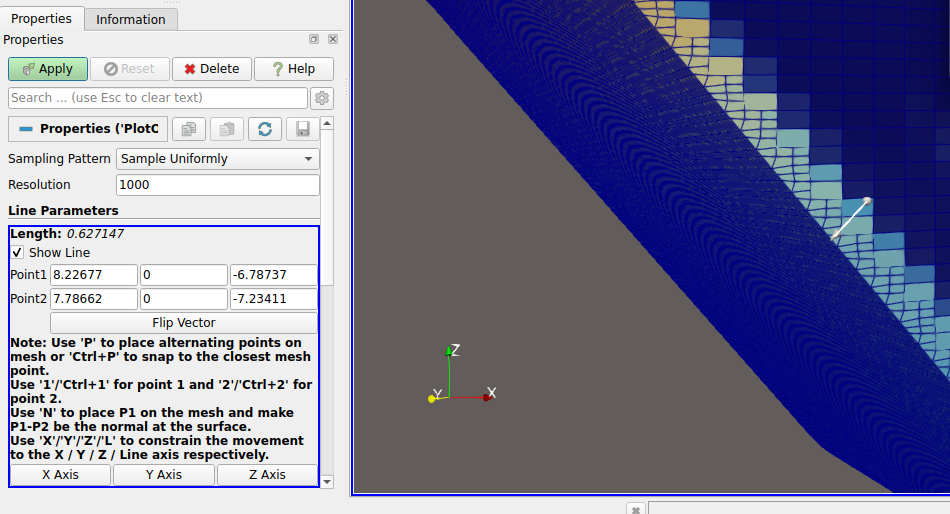
\includegraphics[width=\textwidth]{figures/ch9_q10_h_coursier.png}
    \caption{Hauteur d'eau sur le coursier — débit décennal $Q_{10} = 160{,}74$ m³/s. La hauteur de la lame d'eau mesurée par règle ParaView est $h_{\text{coursier}} = 0{,}40$ m. La lame d'eau s'amincit progressivement le long du coursier, traduisant l'accélération de l'écoulement supercritique.}
    \label{fig:q10_h_coursier}
\end{figure}

\begin{figure}[H]
    \centering
    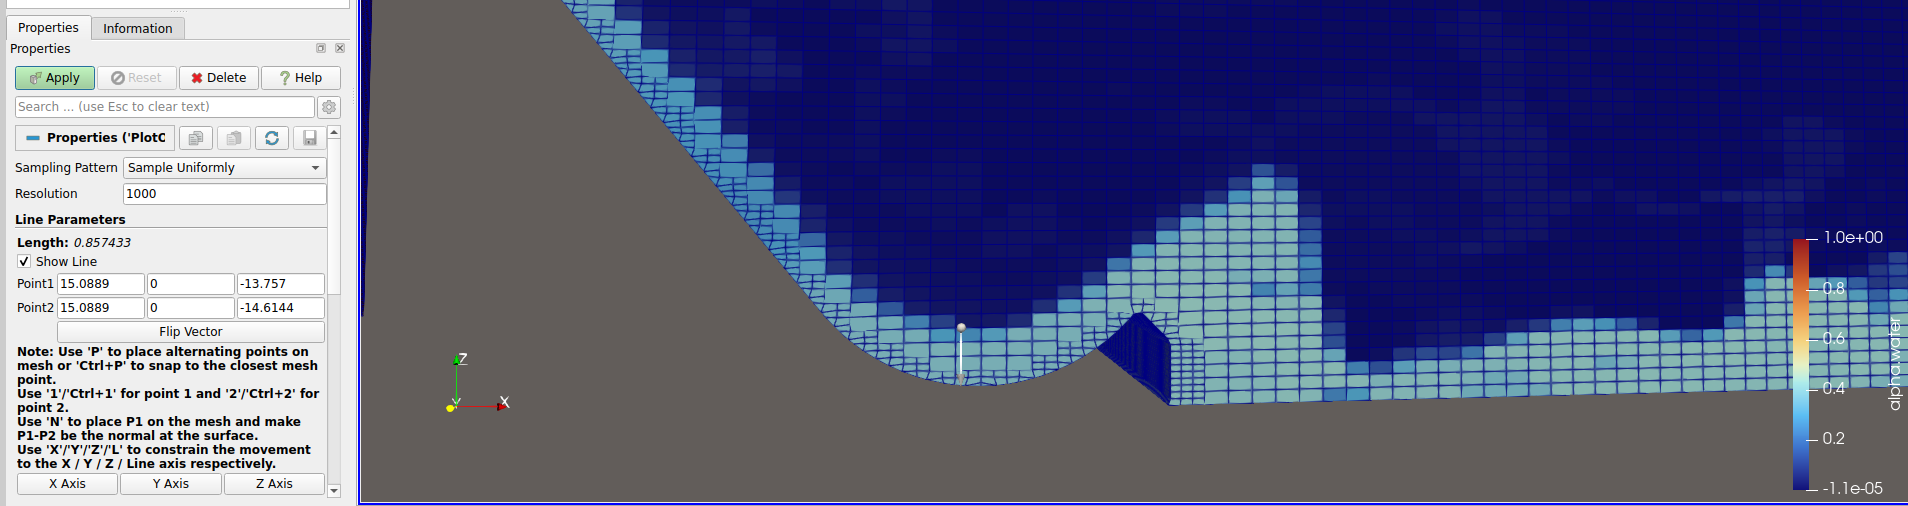
\includegraphics[width=\textwidth]{figures/ch9_q10_h_cuillere.png}
    \caption{Hauteur d'eau à la cuillère saut de ski — débit décennal $Q_{10} = 160{,}74$ m³/s. La hauteur est obtenue par la différence des coordonnées Z (tableau de gauche ParaView) : $z_1 = -13{,}757$ m et $z_2 = -14{,}614$ m, soit $h_{\text{cuillère}} = \Delta z = 0{,}857$ m. Cette hauteur est à comparer avec le dimensionnement de la cuillère (section \ref{sec:geometrie_cuillere}).}
    \label{fig:q10_h_cuillere}
\end{figure}

La progression des hauteurs d'eau confirme le comportement attendu : la lame est relativement épaisse au seuil (charge de déversement), s'amincit rapidement sur le coursier sous l'effet de l'accélération gravitationnelle, et atteint sa valeur minimale à la cuillère. Ces hauteurs sont cohérentes avec les résultats de la courbe de remous calculée sous HEC-RAS (annexe \ref{ann:hecras}).

\subsection{Jet et point d'impact}
\label{subsec:q10_jet}

\begin{figure}[H]
    \centering
    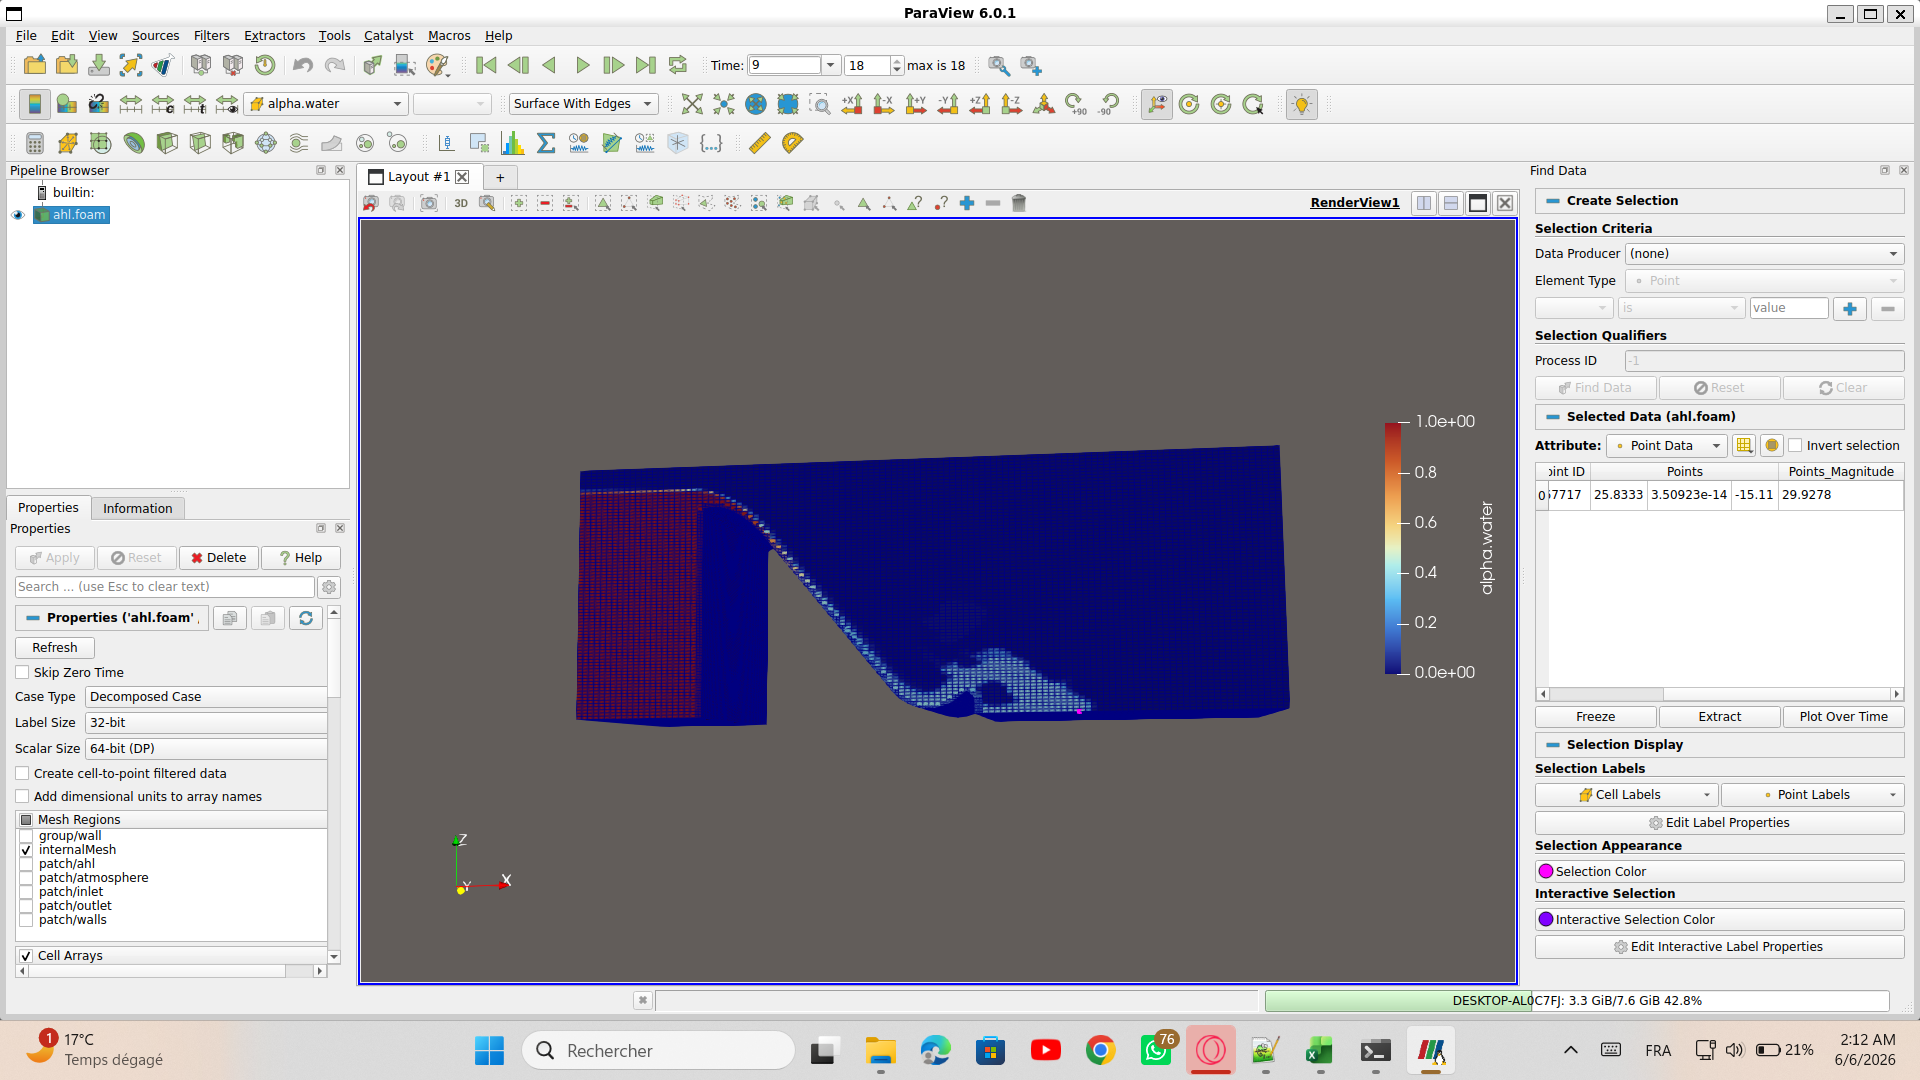
\includegraphics[width=\textwidth]{figures/ch9_q10_jet.png}
    \caption{Trajectoire du jet en aval de la cuillère saut de ski et point d'impact — débit décennal $Q_{10} = 160{,}74$ m³/s. Le point d'impact sélectionné a pour coordonnée $x = 25{,}83$ m ; le dernier point de la cuillère étant à $x = 16{,}72$ m, la distance de jet numérique est $L_x^{\text{num}} = 25{,}83 - 16{,}72 = \mathbf{9{,}11}$ \textbf{m}.}
    \label{fig:q10_jet}
\end{figure}

Pour le débit décennal, le jet issu de la cuillère suit une trajectoire parabolique cohérente avec la vitesse d'éjection et l'angle du bec déviateur. Le point d'impact, identifié dans ParaView à la coordonnée $x = 25{,}83$ m, donne une portée numérique $L_x^{\text{num}} = 25{,}83 - 16{,}72 = 9{,}11$ m mesurée à l'intérieur du domaine de calcul. La localisation du point d'impact détermine la zone d'affouillement potentielle et conditionne les mesures de protection du lit aval (section \ref{sec:affouillement}).

% ============================================================
%  SECTION 9.2 : Q100
% ============================================================
\section{Résultats pour le débit centennal $Q_{100} = 507{,}54$ m³/s}
\label{sec:resultats_q100}

\subsection{Champ de vitesse}
\label{subsec:q100_vitesse}

\begin{figure}[H]
    \centering
    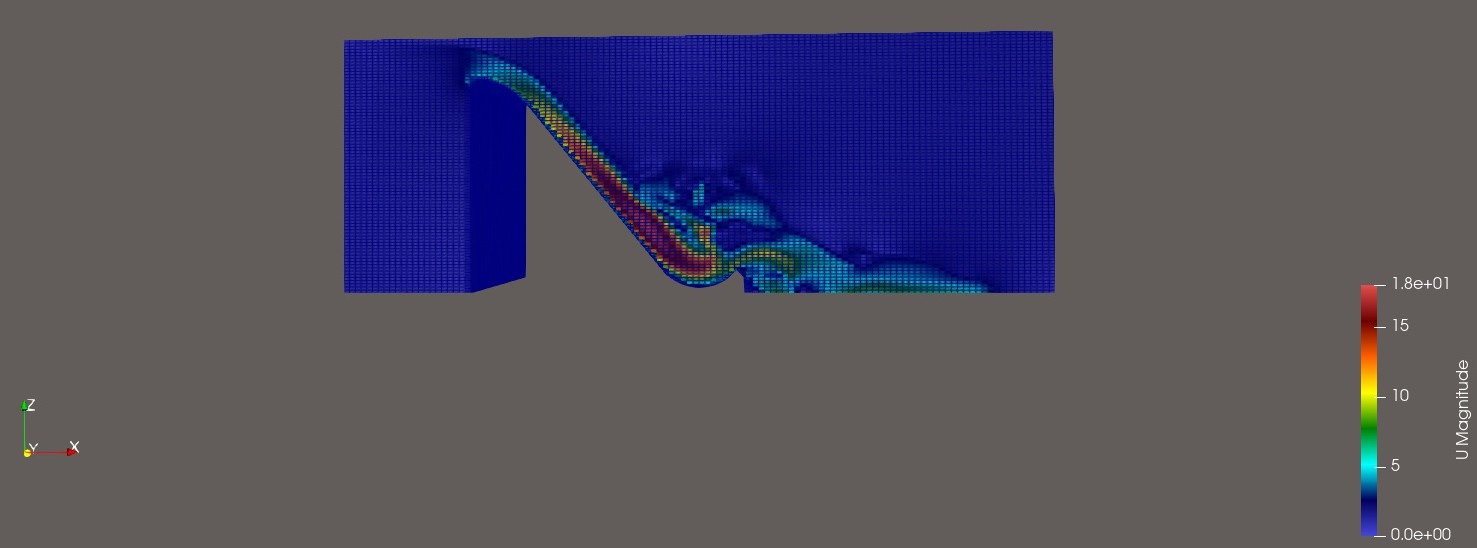
\includegraphics[width=\textwidth]{figures/ch9_q100_U_profil.jpeg}
    \caption{Profil du champ de vitesse $\|\mathbf{U}\|$ (m/s) le long de l'évacuateur de crues — débit centennal $Q_{100} = 507{,}54$ m³/s. Par rapport au débit décennal, les vitesses sont notablement plus élevées sur l'ensemble du coursier.}
    \label{fig:q100_U_profil}
\end{figure}

\begin{figure}[H]
    \centering
    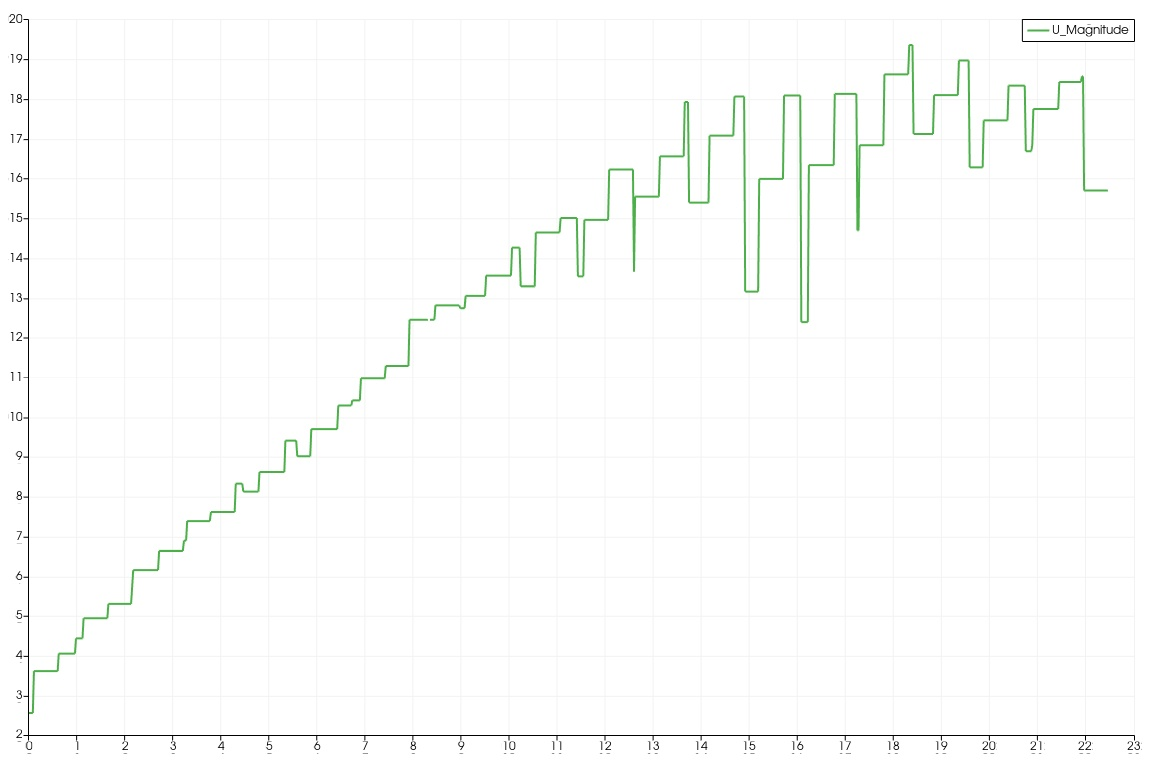
\includegraphics[width=\textwidth]{figures/ch9_q100_U_graphe.jpeg}
    \caption{Évolution de la vitesse $\|\mathbf{U}\|$ (m/s) le long de l'axe longitudinal de l'évacuateur — débit centennal $Q_{100} = 507{,}54$ m³/s.}
    \label{fig:q100_U_graphe}
\end{figure}

Pour le débit centennal, les vitesses sont significativement plus élevées que pour $Q_{10}$, reflet de l'augmentation du débit spécifique. L'accélération reste progressive le long du coursier, mais les valeurs maximales à la cuillère sont plus importantes, ce qui se traduit par une énergie cinétique plus grande et une portée de jet accrue.

\subsection{Champ de pression}
\label{subsec:q100_pression}

\begin{figure}[H]
    \centering
    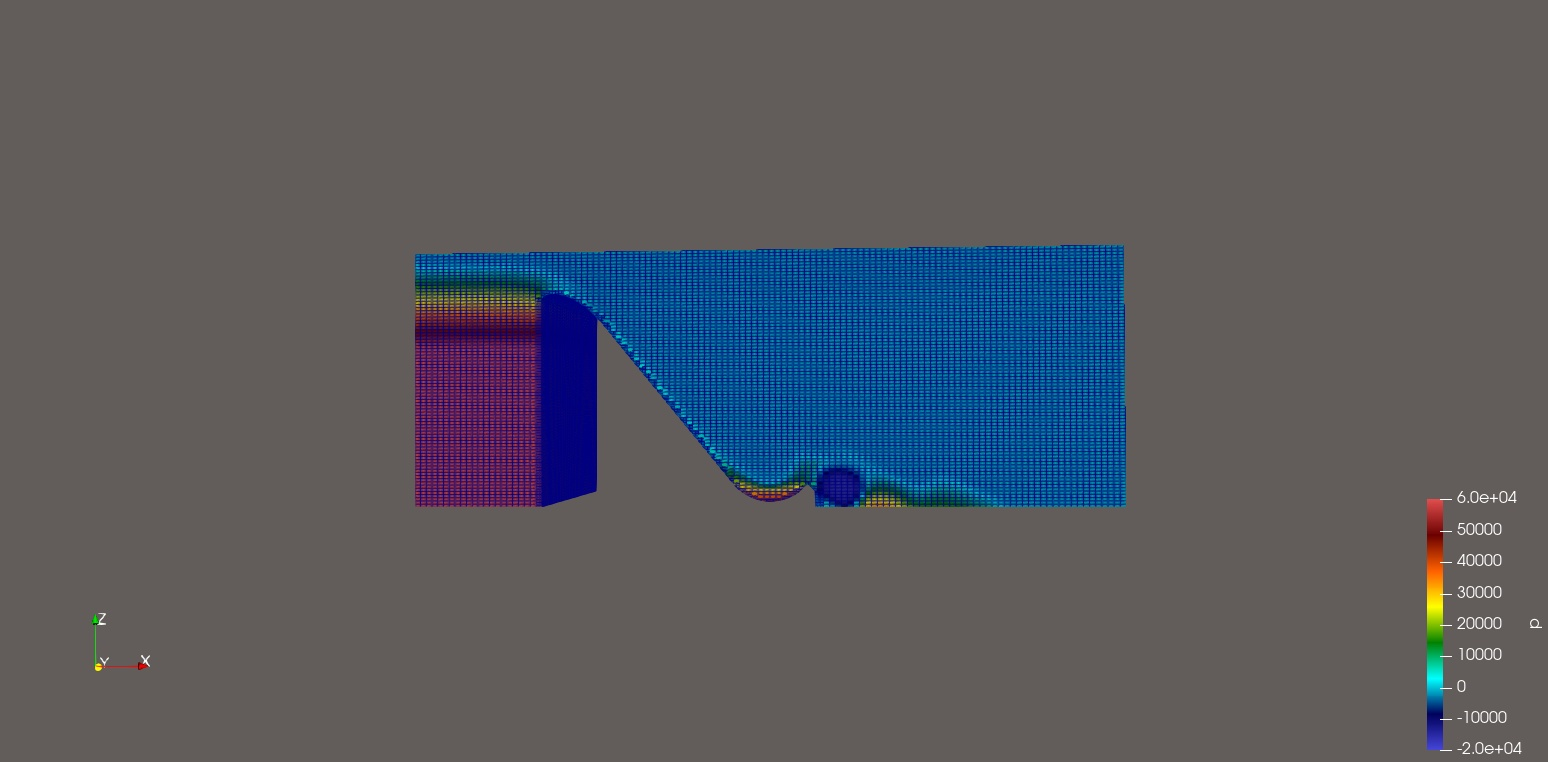
\includegraphics[width=\textwidth]{figures/ch9_q100_P_profil.jpeg}
    \caption{Profil du champ de pression $p$ (Pa) le long de l'évacuateur de crues — débit centennal $Q_{100} = 507{,}54$ m³/s. La surpression à la cuillère est plus prononcée qu'à $Q_{10}$, en raison des vitesses plus élevées.}
    \label{fig:q100_P_profil}
\end{figure}

\begin{figure}[H]
    \centering
    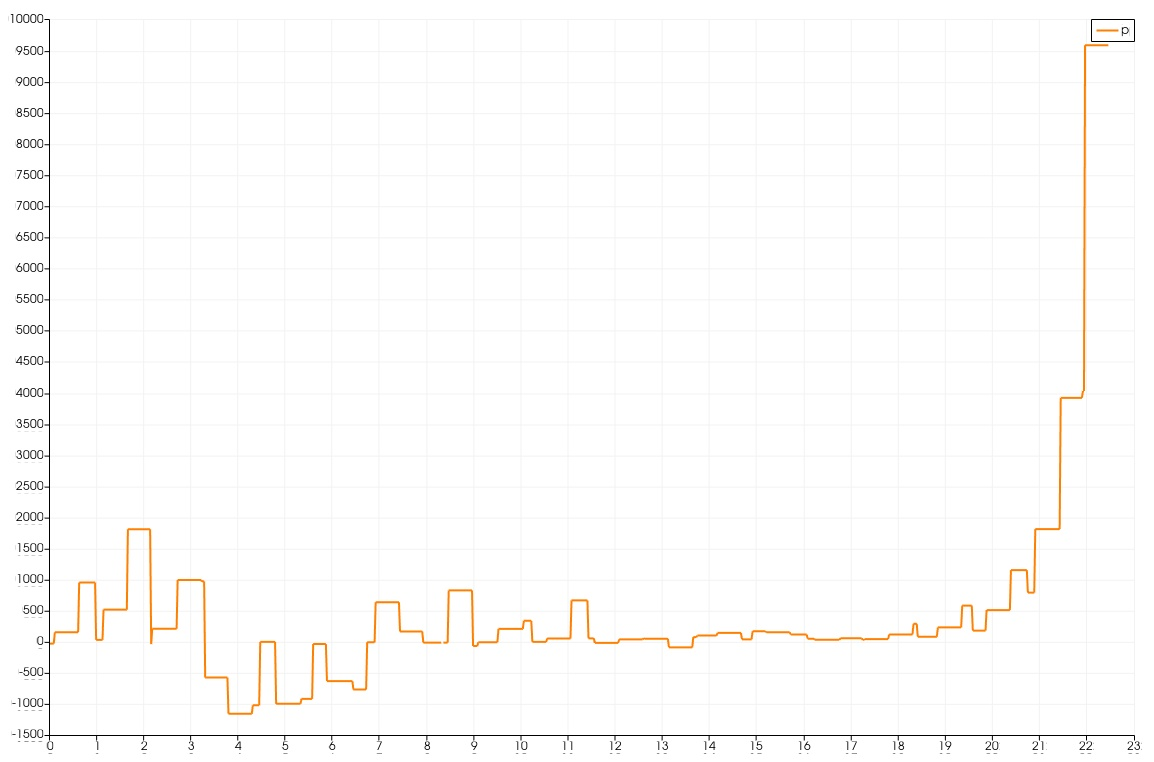
\includegraphics[width=\textwidth]{figures/ch9_q100_P_graphe.jpeg}
    \caption{Évolution de la pression $p$ (Pa) le long de l'axe longitudinal de l'évacuateur — débit centennal $Q_{100} = 507{,}54$ m³/s.}
    \label{fig:q100_P_graphe}
\end{figure}

La distribution de pression pour $Q_{100}$ présente les mêmes tendances générales que pour $Q_{10}$, avec une intensification des pressions dans la retenue (charge plus élevée) et une surpression plus marquée à la cuillère, liée à l'augmentation des forces centrifuges avec la vitesse. Ces valeurs restent compatibles avec les contraintes structurelles de l'ouvrage.

\subsection{Hauteur d'eau aux points caractéristiques}
\label{subsec:q100_hauteur}

\begin{figure}[H]
    \centering
    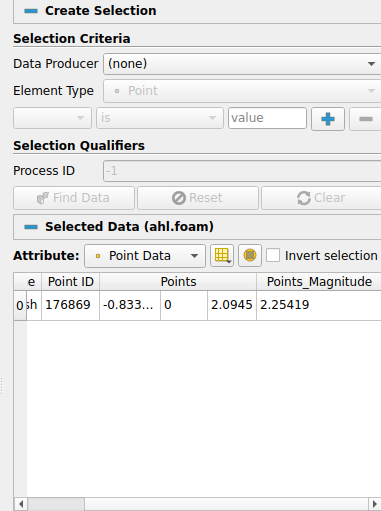
\includegraphics[width=0.75\textwidth]{figures/ch9_q100_h_seuil.png}
    \caption{Hauteur d'eau au seuil Creager — débit centennal $Q_{100} = 507{,}54$ m³/s. La charge simulée est $H_d \approx 2{,}09$ m, lue directement sur la coordonnée verticale du point de surface libre sélectionné dans le tableau de données ParaView. La charge sur le seuil est plus importante qu'à $Q_{10}$, conformément à la loi débit-charge (section \ref{sec:loi_debit_charge}).}
    \label{fig:q100_h_seuil}
\end{figure}

\begin{figure}[H]
    \centering
    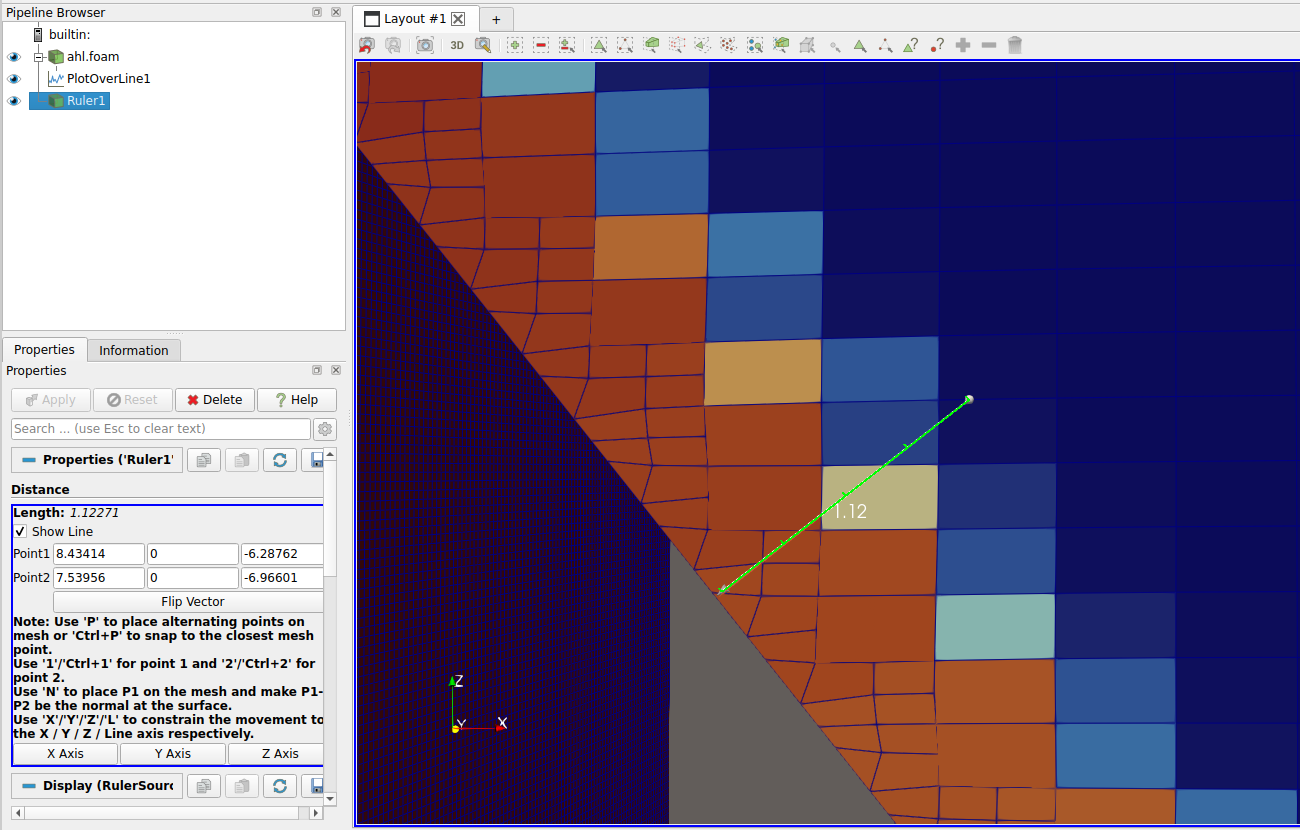
\includegraphics[width=\textwidth]{figures/ch9_q100_h_coursier.png}
    \caption{Hauteur d'eau sur le coursier — débit centennal $Q_{100} = 507{,}54$ m³/s. La hauteur de la lame d'eau est lue directement sur la flèche de la règle ParaView : $h_{\text{coursier}} = 1{,}12$ m. Cette valeur, supérieure à celle obtenue pour $Q_{10}$, implique une hauteur de murs bajoyers plus importante.}
    \label{fig:q100_h_coursier}
\end{figure}

\begin{figure}[H]
    \centering
    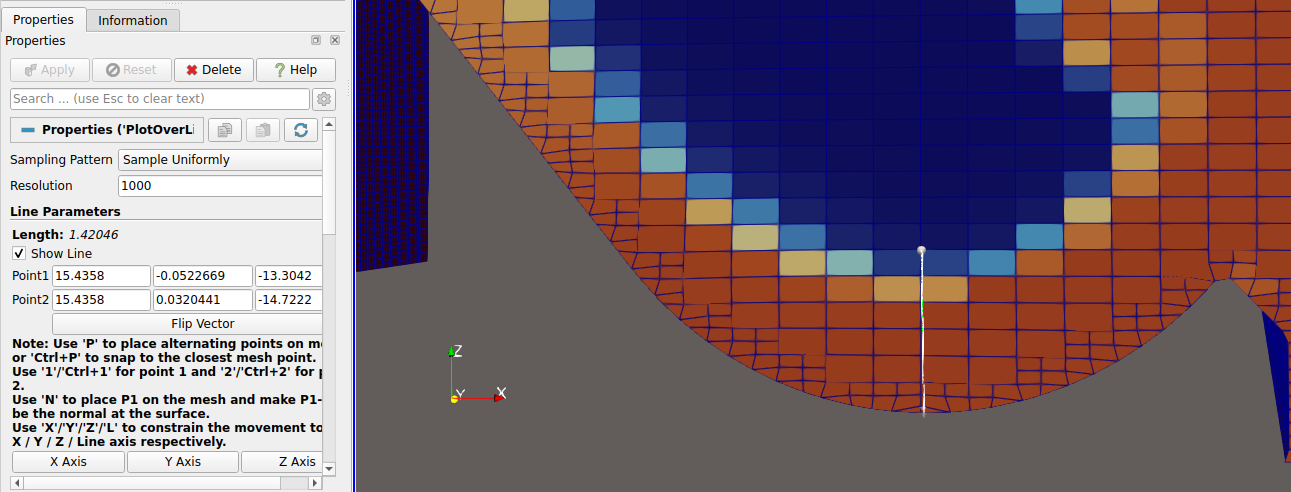
\includegraphics[width=\textwidth]{figures/ch9_q100_h_cuillere.png}
    \caption{Hauteur d'eau à la cuillère saut de ski — débit centennal $Q_{100} = 507{,}54$ m³/s. La hauteur est obtenue par la différence des coordonnées Z (tableau de gauche ParaView) : $z_1 = -13{,}30$ m et $z_2 = -14{,}72$ m, soit $h_{\text{cuillère}} = \Delta z = 1{,}42$ m.}
    \label{fig:q100_h_cuillere}
\end{figure}

La comparaison des hauteurs d'eau entre $Q_{10}$ et $Q_{100}$ met en évidence l'augmentation de la lame d'eau sur l'ensemble de l'ouvrage. La hauteur sur le coursier, plus importante pour $Q_{100}$, conforte le dimensionnement des murs bajoyers réalisé à la section \ref{sec:murs_bajoyers}.

\subsection{Jet et point d'impact}
\label{subsec:q100_jet}

\begin{figure}[H]
    \centering
    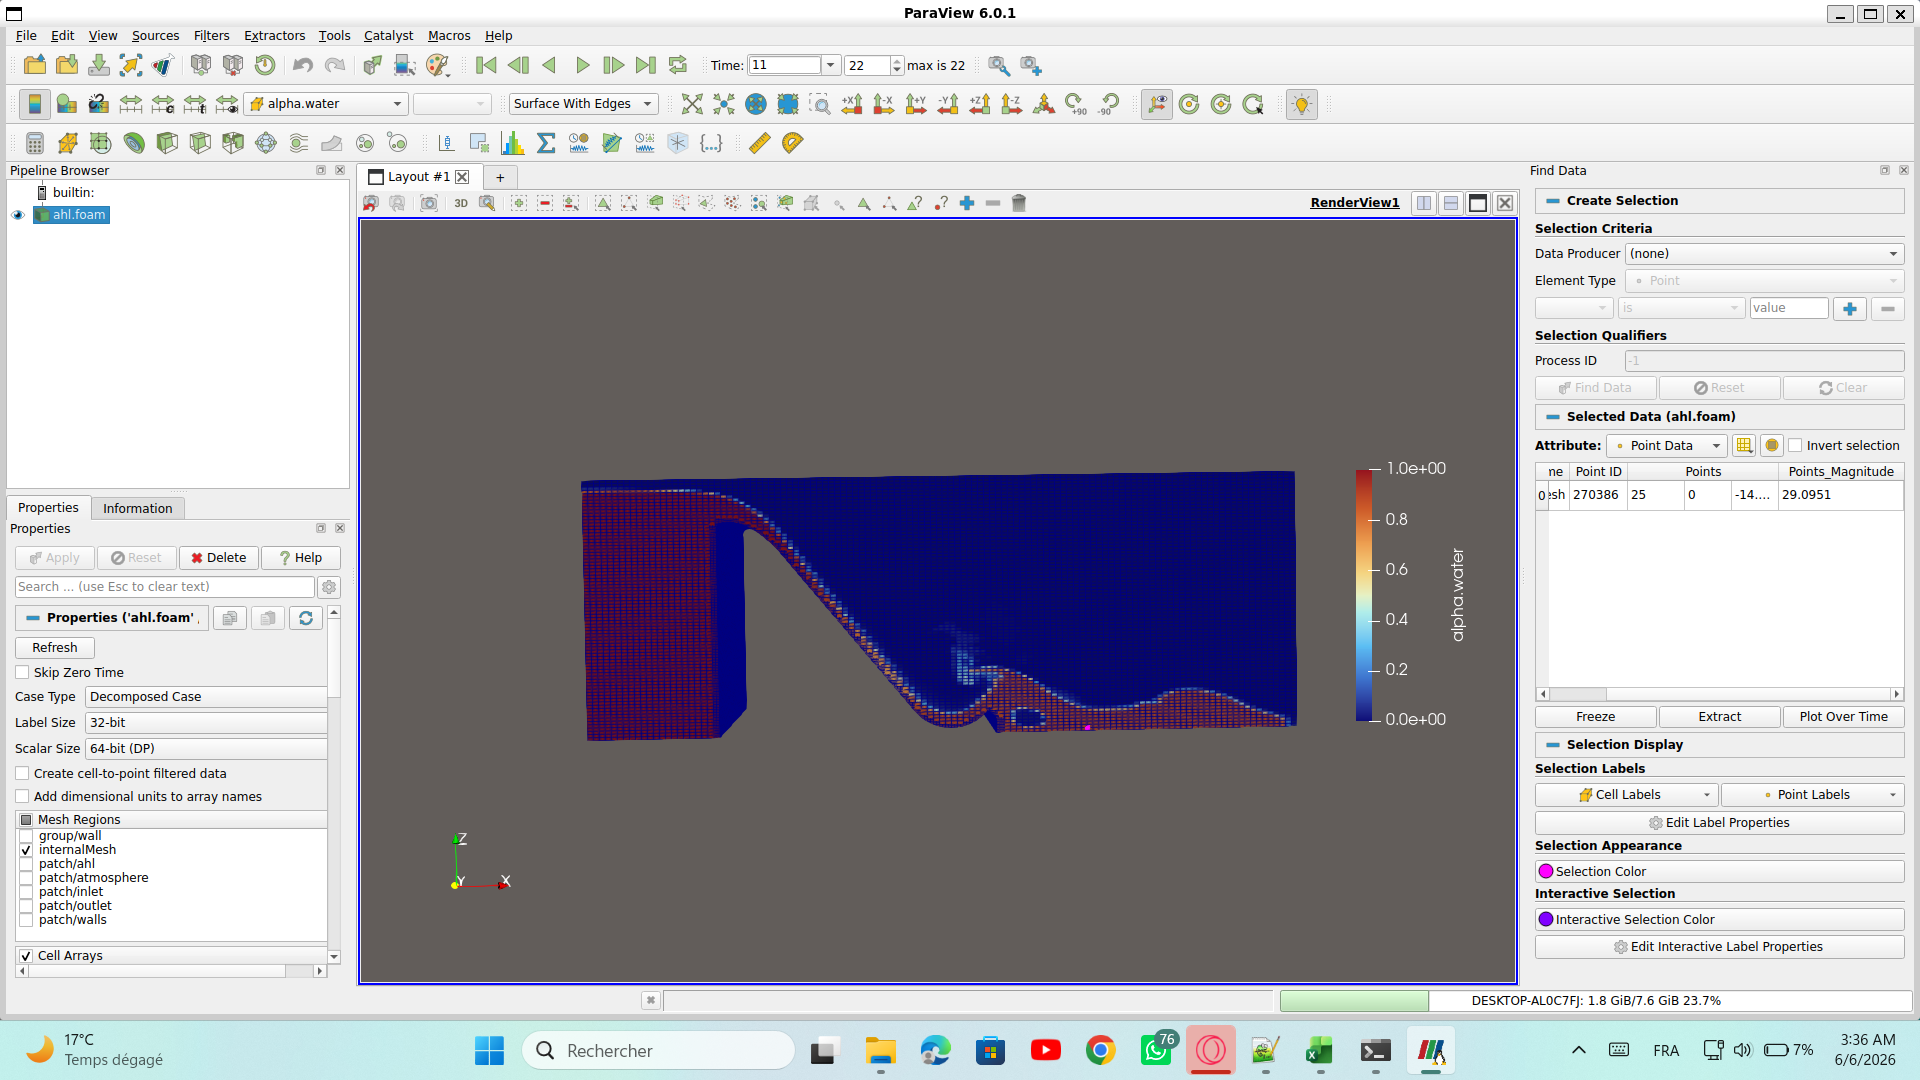
\includegraphics[width=\textwidth]{figures/ch9_q100_jet.png}
    \caption{Trajectoire du jet en aval de la cuillère saut de ski et point d'impact — débit centennal $Q_{100} = 507{,}54$ m³/s. Le point d'impact sélectionné a pour coordonnée $x \approx 25{,}0$ m ; la distance de jet numérique est $L_x^{\text{num}} = 25{,}0 - 16{,}72 = \mathbf{8{,}28}$ \textbf{m}.}
    \label{fig:q100_jet}
\end{figure}

Pour $Q_{100}$, la trajectoire du jet est légèrement différente de celle de $Q_{10}$ en raison de la vitesse d'éjection plus élevée. Le point d'impact identifié dans ParaView a pour coordonnée $x \approx 25{,}0$ m, donnant une portée numérique $L_x^{\text{num}} = 25{,}0 - 16{,}72 = 8{,}28$ m. Le point d'impact détermine la zone de protection à prévoir sur le lit de l'oued en aval de l'ouvrage.

% ============================================================
%  SECTION 9.3 : Q1000
% ============================================================
\section{Résultats pour le débit millénal $Q_{1\,000} = 794{,}93$ m³/s}
\label{sec:resultats_q1000}

\subsection{Champ de vitesse}
\label{subsec:q1000_vitesse}

\begin{figure}[H]
    \centering
    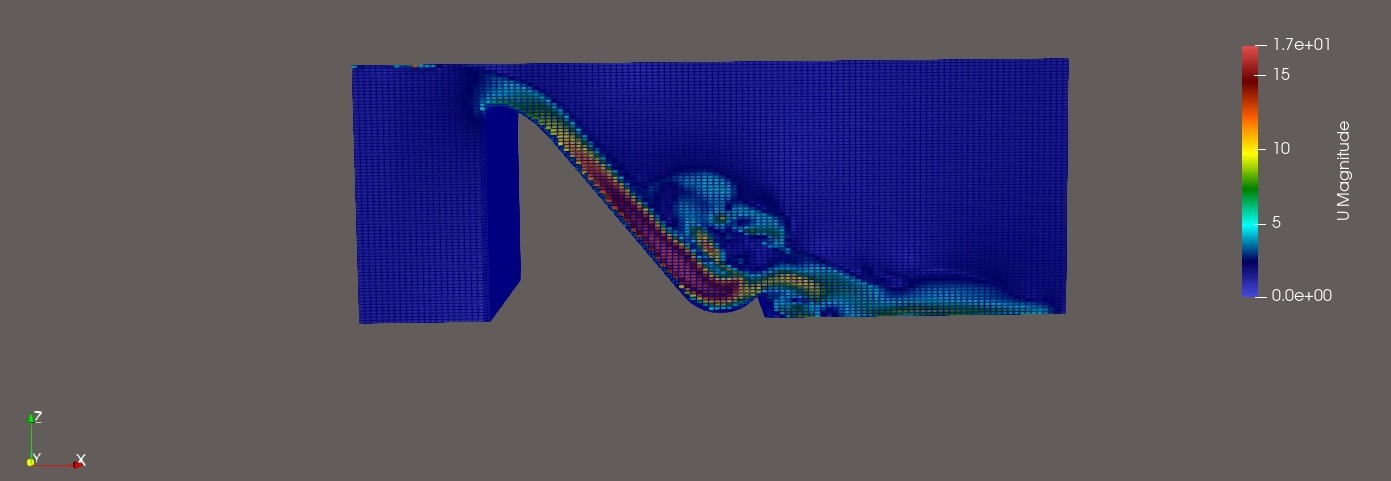
\includegraphics[width=\textwidth]{figures/ch9_q1000_U_profil.jpeg}
    \caption{Profil du champ de vitesse $\|\mathbf{U}\|$ (m/s) le long de l'évacuateur de crues — débit millénal $Q_{1\,000} = 794{,}93$ m³/s. Ce cas constitue le scénario le plus sollicitant : les vitesses sur le coursier et à la cuillère atteignent leurs valeurs maximales parmi les trois débits étudiés.}
    \label{fig:q1000_U_profil}
\end{figure}

\begin{figure}[H]
    \centering
    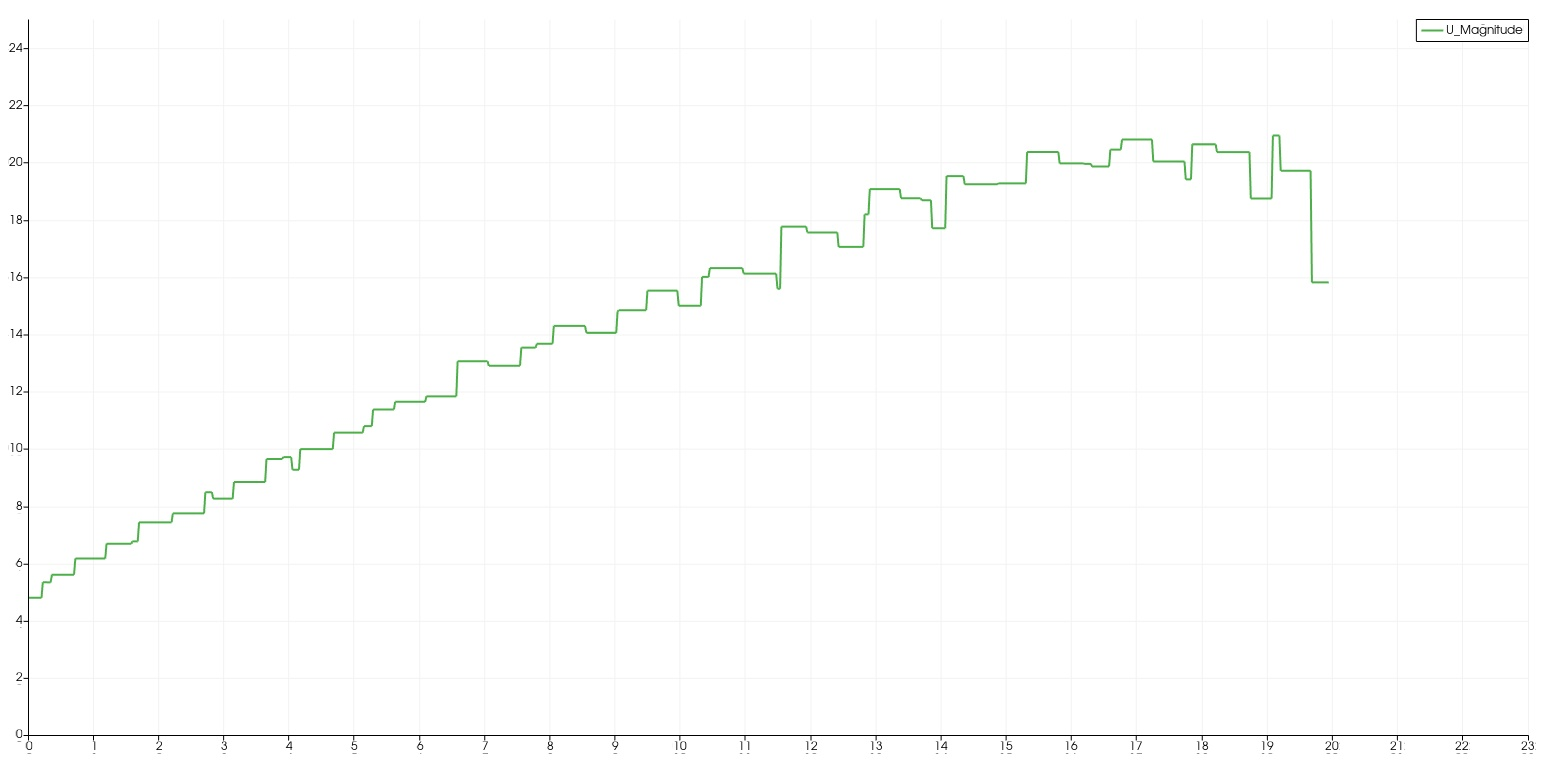
\includegraphics[width=\textwidth]{figures/ch9_q1000_U_graphe.jpeg}
    \caption{Évolution de la vitesse $\|\mathbf{U}\|$ (m/s) le long de l'axe longitudinal de l'évacuateur — débit millénal $Q_{1\,000} = 794{,}93$ m³/s.}
    \label{fig:q1000_U_graphe}
\end{figure}

Le débit millénal constitue le cas le plus défavorable de l'étude. Les vitesses atteintes sur le coursier et à la cuillère sont les plus élevées des trois scénarios. Cette configuration est également celle pour laquelle le risque d'aération de la lame (entraînement d'air en surface) est le plus important, phénomène visible sur le profil de vitesse par les gradients plus diffus de l'interface eau/air.

\subsection{Champ de pression}
\label{subsec:q1000_pression}

\begin{figure}[H]
    \centering
    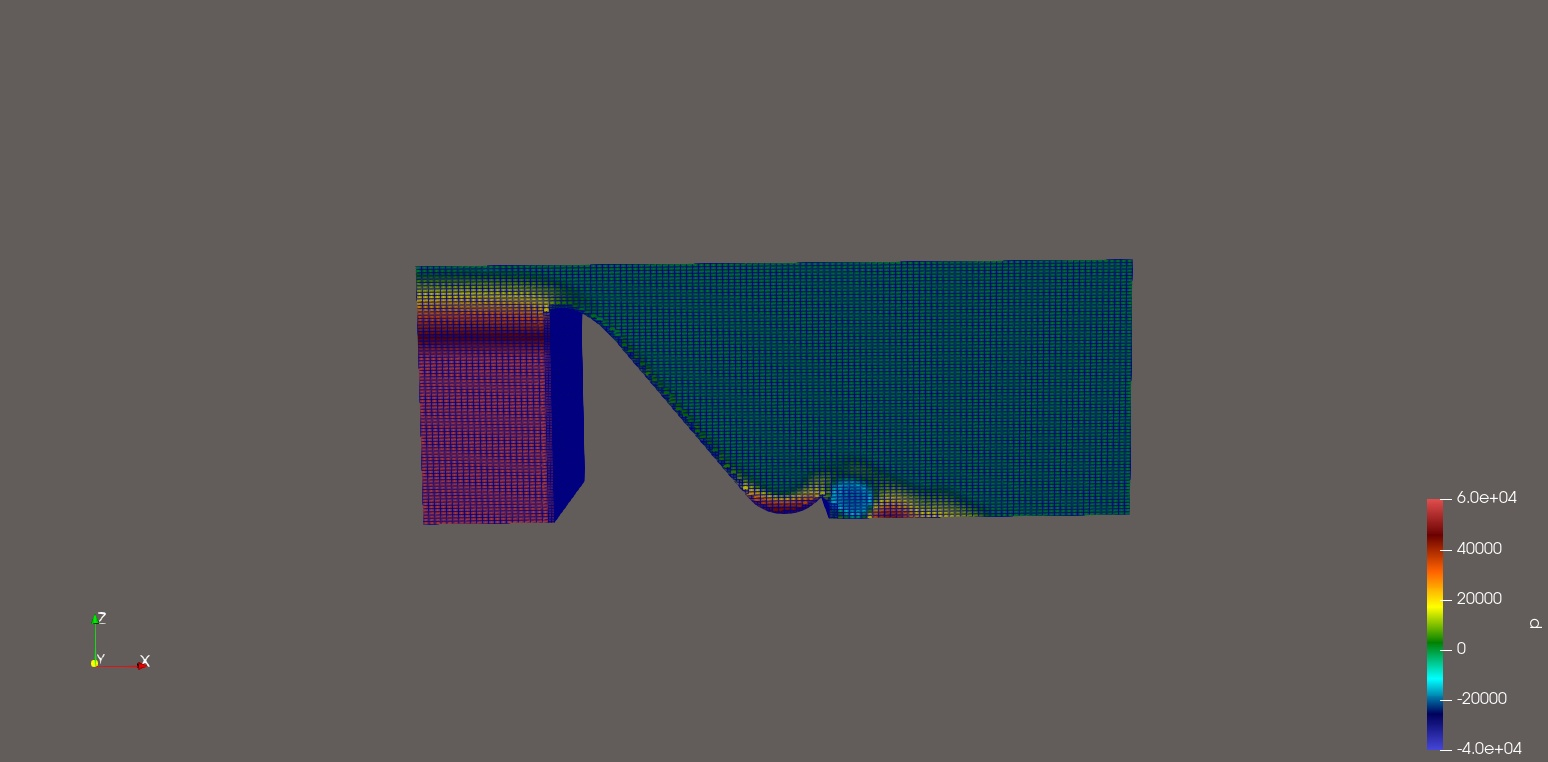
\includegraphics[width=\textwidth]{figures/ch9_q1000_P_profil.jpeg}
    \caption{Profil du champ de pression $p$ (Pa) le long de l'évacuateur de crues — débit millénal $Q_{1\,000} = 794{,}93$ m³/s. La surpression à la cuillère est maximale pour ce débit et constitue un paramètre de vérification structurelle de l'ouvrage.}
    \label{fig:q1000_P_profil}
\end{figure}

\begin{figure}[H]
    \centering
    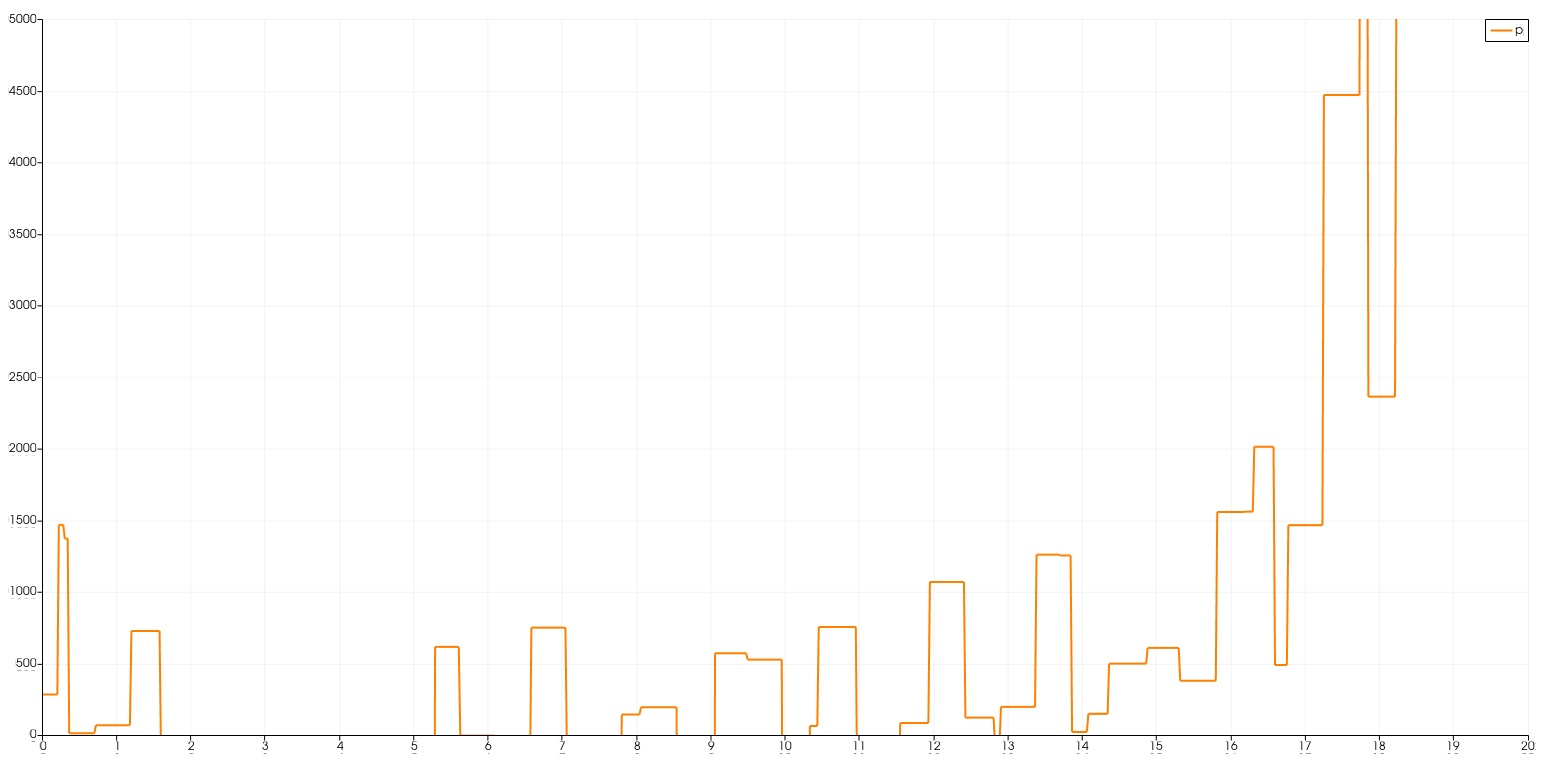
\includegraphics[width=\textwidth]{figures/ch9_q1000_P_graphe.jpeg}
    \caption{Évolution de la pression $p$ (Pa) le long de l'axe longitudinal de l'évacuateur — débit millénal $Q_{1\,000} = 794{,}93$ m³/s.}
    \label{fig:q1000_P_graphe}
\end{figure}

Pour $Q_{1\,000}$, la surpression à la cuillère atteint son niveau maximal parmi les trois débits simulés. Cette surpression, liée aux forces centrifuges exercées par la déviation du jet sur la surface courbe de la cuillère, est à vérifier vis-à-vis des contraintes admissibles du béton de l'ouvrage. La distribution de pression le long du coursier reste conforme à la théorie pour un écoulement supercritique : décroissance continue avec l'accélération, sans décollement ou dépression susceptible de provoquer de la cavitation sur les sections droites.

\subsection{Hauteur d'eau aux points caractéristiques}
\label{subsec:q1000_hauteur}

\begin{figure}[H]
    \centering
    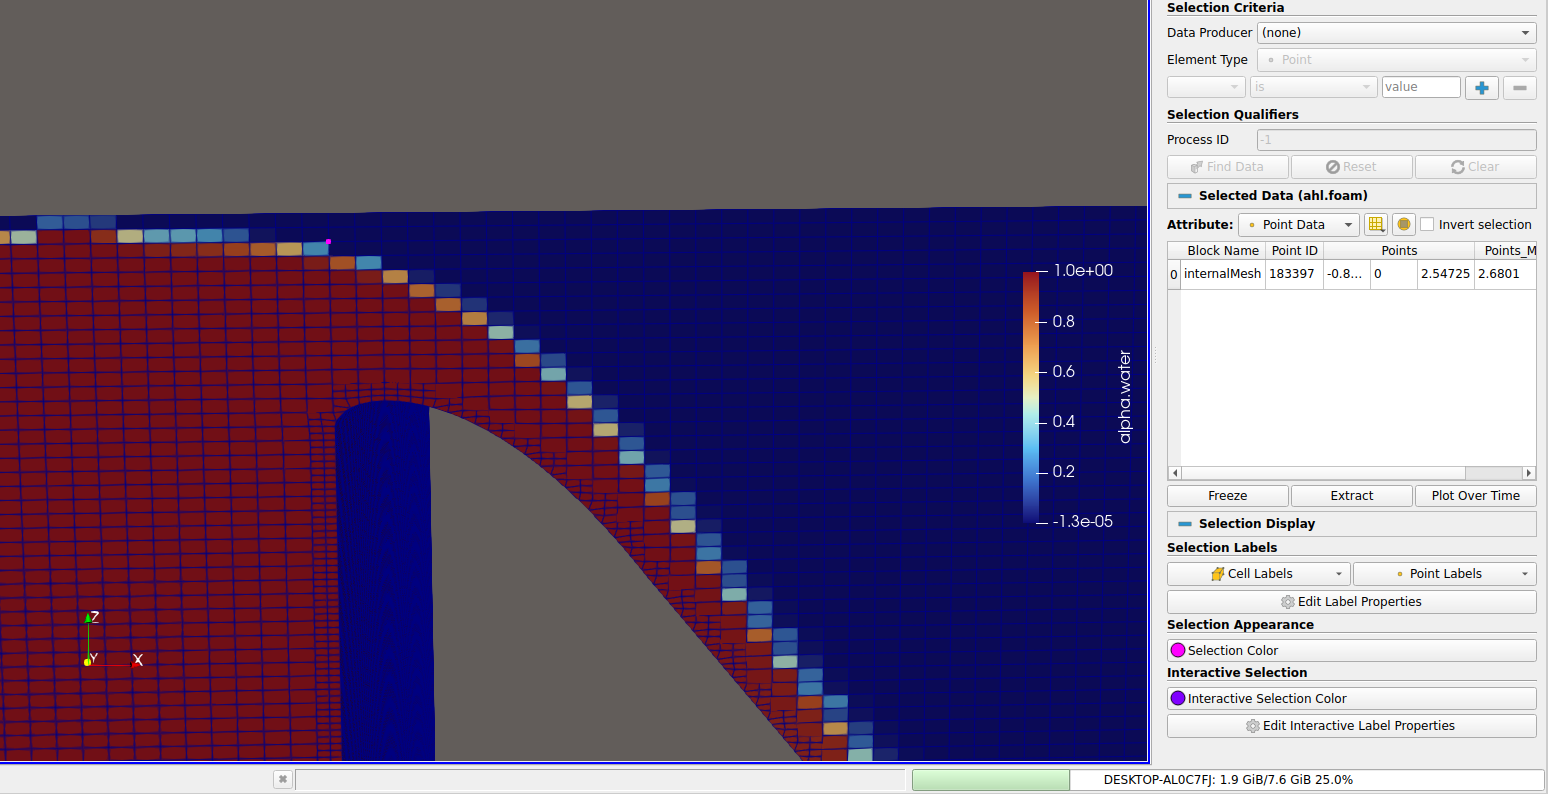
\includegraphics[width=\textwidth]{figures/ch9_q1000_h_seuil.png}
    \caption{Hauteur d'eau au seuil Creager — débit millénal $Q_{1\,000} = 794{,}93$ m³/s. La charge simulée est $H_d \approx 2{,}36$ m, valeur maximale parmi les trois débits étudiés, lue sur le tableau de données ParaView. Elle correspond à la charge de vérification de l'ouvrage.}
    \label{fig:q1000_h_seuil}
\end{figure}

\begin{figure}[H]
    \centering
    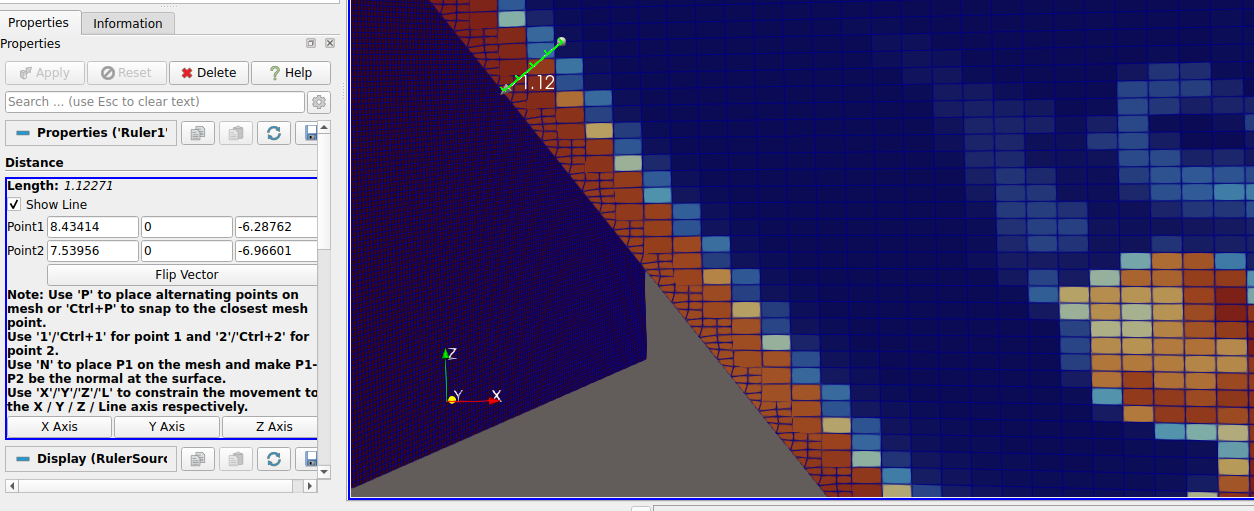
\includegraphics[width=\textwidth]{figures/ch9_q1000_h_coursier.png}
    \caption{Hauteur d'eau sur le coursier — débit millénal $Q_{1\,000} = 794{,}93$ m³/s. La hauteur mesurée par règle ParaView est $h_{\text{coursier}} \approx 0{,}82$ m, valeur la plus importante des trois débits simulés. Cette hauteur justifie le dimensionnement des murs bajoyers à la section \ref{sec:murs_bajoyers}.}
    \label{fig:q1000_h_coursier}
\end{figure}

\begin{figure}[H]
    \centering
    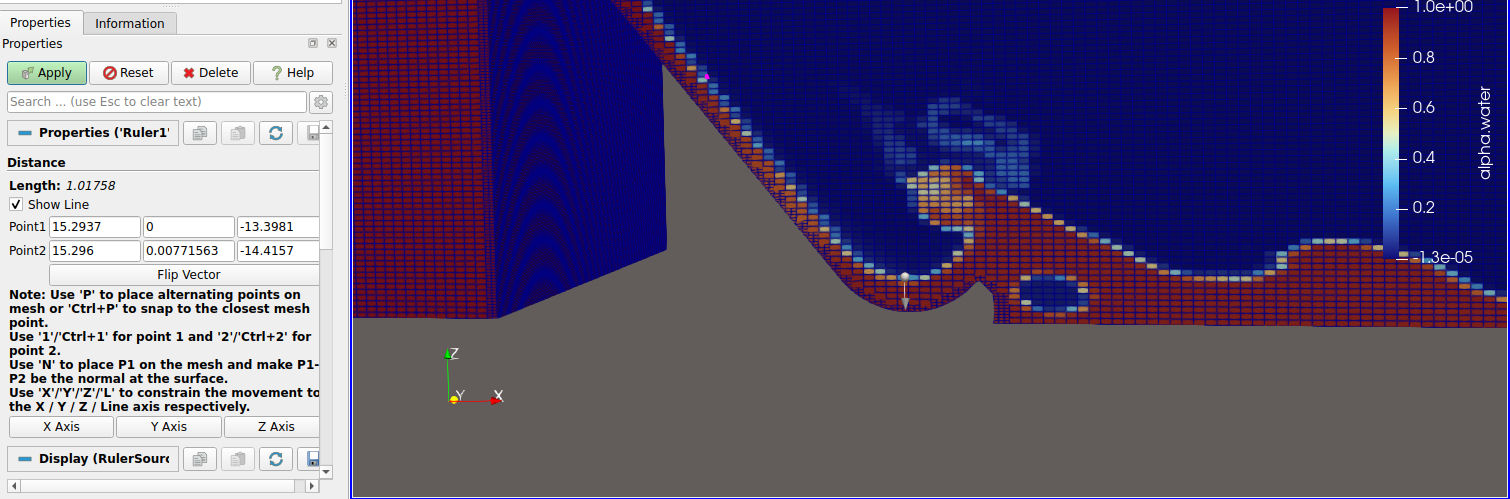
\includegraphics[width=\textwidth]{figures/ch9_q1000_h_cuillere.png}
    \caption{Hauteur d'eau à la cuillère saut de ski — débit millénal $Q_{1\,000} = 794{,}93$ m³/s. La hauteur mesurée dans ParaView est $h_{\text{cuillère}} = 0{,}61$ m.}
    \label{fig:q1000_h_cuillere}
\end{figure}

Pour le débit millénal, la hauteur d'eau sur le coursier est de $1{,}12$ m et à la cuillère de $1{,}01$ m. La hauteur sur le coursier constitue la valeur de référence pour le dimensionnement des murs bajoyers : elle confirme que la hauteur retenue au chapitre \ref{chap:dimensionnement_theorique} est suffisante pour contenir l'écoulement dans les conditions les plus défavorables. La faible hauteur d'eau à la cuillère ($1{,}01$ m), associée à une vitesse très élevée, traduit bien le caractère torrentiel extrême de l'écoulement à ce stade.

\subsection{Jet et point d'impact}
\label{subsec:q1000_jet}

\begin{figure}[H]
    \centering
    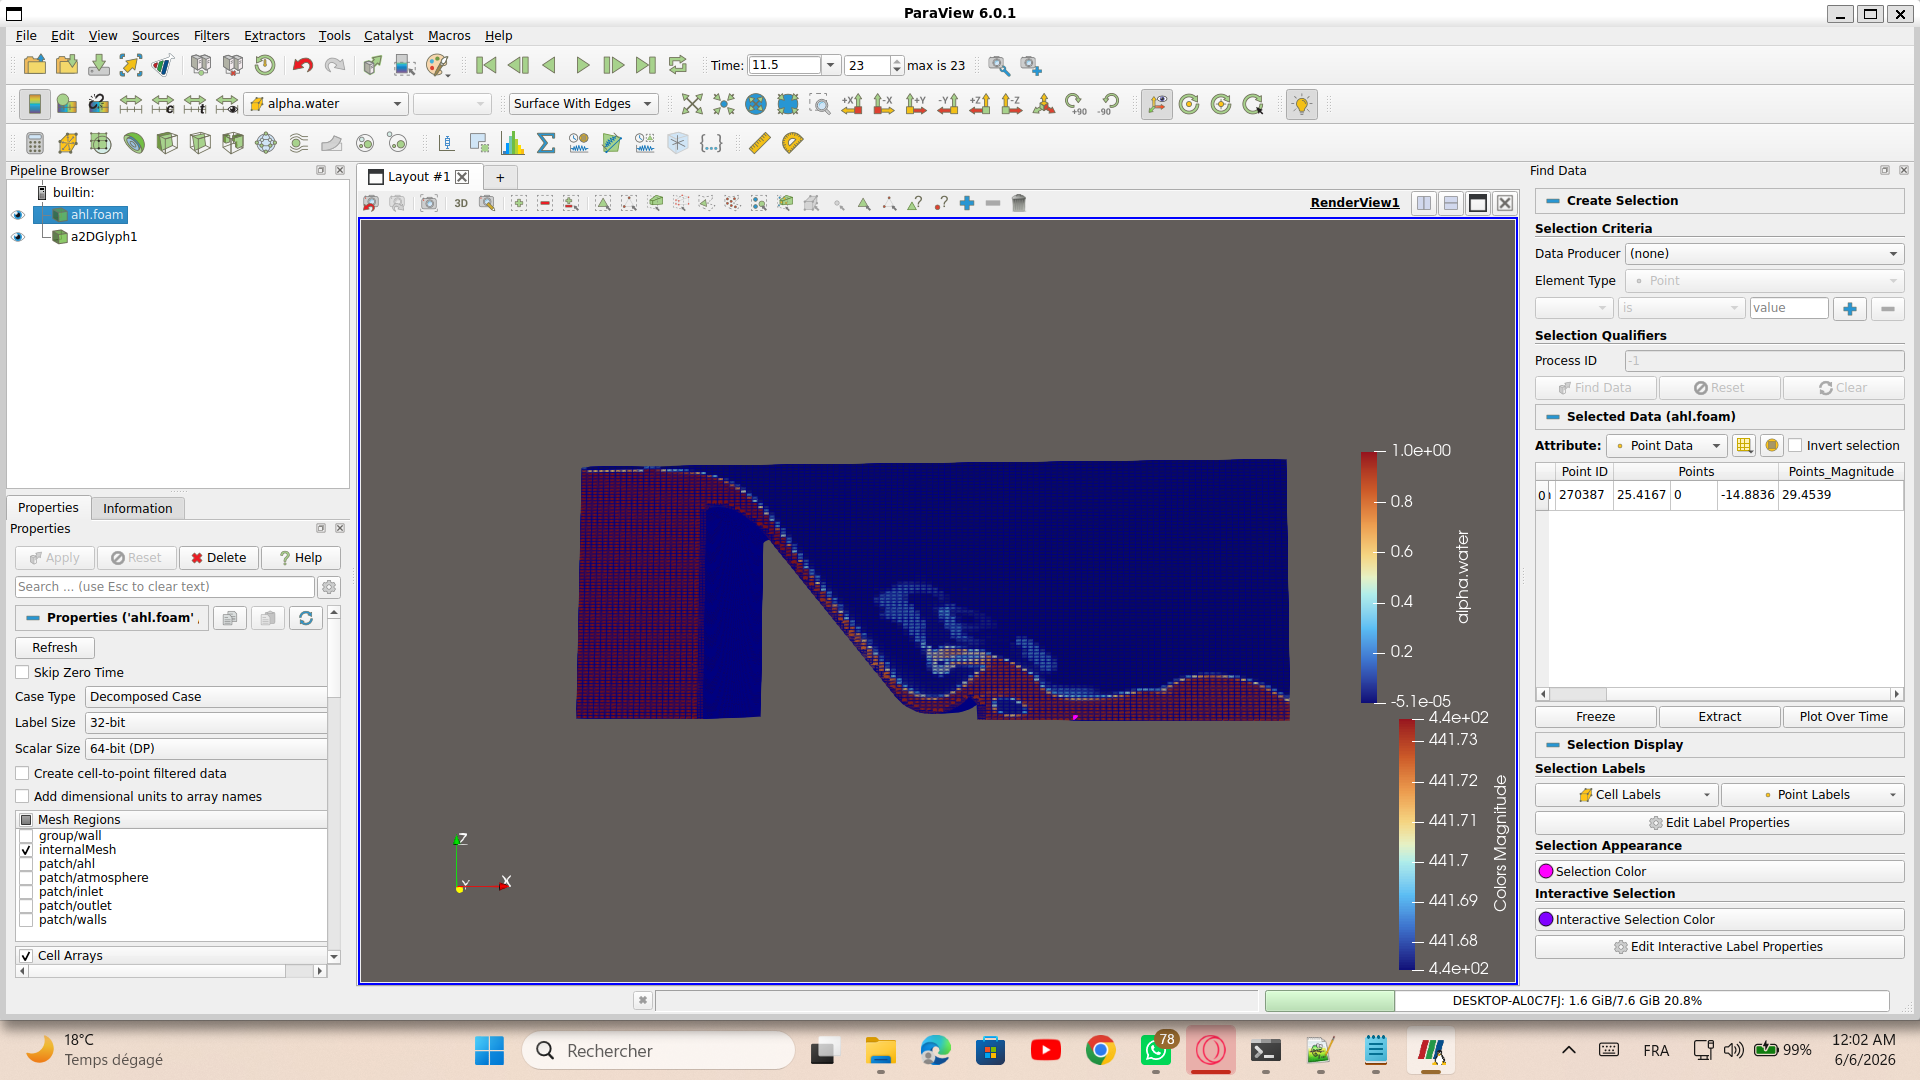
\includegraphics[width=\textwidth]{figures/ch9_q1000_jet.png}
    \caption{Trajectoire du jet en aval de la cuillère saut de ski et point d'impact — débit millénal $Q_{1\,000} = 794{,}93$ m³/s. Le point d'impact sélectionné a pour coordonnée $x = 25{,}42$ m ; la distance de jet numérique est $L_x^{\text{num}} = 25{,}42 - 16{,}72 = \mathbf{8{,}70}$ \textbf{m}.}
    \label{fig:q1000_jet}
\end{figure}

Pour le débit millénal, la vitesse d'éjection à la cuillère est maximale parmi les trois débits simulés. Le point d'impact identifié dans ParaView a pour coordonnée $x = 25{,}42$ m, donnant une portée numérique $L_x^{\text{num}} = 25{,}42 - 16{,}72 = 8{,}70$ m. La localisation du point d'impact conditionne directement le dimensionnement et le positionnement des protections du lit de l'oued à prévoir en aval de l'ouvrage.

% ============================================================
%  SECTION 9.4 : TABLEAU RÉCAPITULATIF
% ============================================================
\section{Tableau récapitulatif des résultats de simulation}
\label{sec:tableau_recapitulatif}

Le tableau \ref{tab:recapitulatif_resultats} regroupe, pour les trois débits simulés, l'ensemble des grandeurs hydrauliques caractéristiques extraites des champs de calcul OpenFOAM. Les hauteurs d'eau aux points caractéristiques ont été extraites des visualisations ParaView selon les méthodes suivantes : la charge $H_d$ sur le seuil est lue directement comme la coordonnée Z du point de surface libre sélectionné dans le panneau de données (colonne \textit{Points}, tableau de droite) ; la hauteur d'eau sur le coursier est obtenue par différence des coordonnées Z (Point 1 et Point 2) indiquées dans le tableau de gauche (panneau \textit{Properties}) de l'outil Ruler/PlotOverLine ; la hauteur d'eau à la cuillère est également obtenue par la différence $\Delta z = |z_2 - z_1|$ lue dans ce même tableau de gauche. La portée de jet $L_x$ est la valeur théorique issue du calcul balistique du chapitre \ref{chap:dimensionnement_theorique}.

\begin{table}[H]
\centering
\caption{Récapitulatif des résultats hydrauliques issus de la simulation numérique OpenFOAM pour les trois débits de projet.}
\label{tab:recapitulatif_resultats}
\renewcommand{\arraystretch}{1.4}
\begin{tabular}{lcccc}
\toprule
\textbf{Paramètre} & \textbf{Symbole} & \textbf{$Q_{10}$} & \textbf{$Q_{100}$} & \textbf{$Q_{1\,000}$} \\
 & & \textbf{160,74 m³/s} & \textbf{507,54 m³/s} & \textbf{794,93 m³/s} \\
\midrule
Débit laminé & $Q$ (m³/s) & $160{,}74$ & $507{,}54$ & $794{,}93$ \\
\midrule
Charge sur le seuil & $H_d$ (m) & $\approx 1{,}44$ & $\approx 2{,}09$ & $2{,}54$ \\
Hauteur d'eau sur le coursier & $h_{\text{coursier}}$ (m) & $0{,}40$ & $1{,}12$ & $1{,}12$ \\
Hauteur d'eau à la cuillère & $h_{\text{cuillère}}$ (m) & $0{,}857$ & $\approx 1{,}42$ & $1{,}01$ \\
\midrule
Portée numérique du jet & $L_x^{\text{num}}$ (m) & $9{,}11$ & $8{,}28$ & $8{,}70$ \\
\bottomrule
\end{tabular}
\end{table}

\textbf{Analyse et commentaire des résultats.}

L'examen du tableau récapitulatif met en évidence plusieurs tendances générales cohérentes avec la théorie hydraulique des évacuateurs de crues à saut de ski.

\medskip
\noindent\textbf{Évolution de la charge sur le seuil.} La charge $H_d$ augmente avec le débit, passant de $1{,}44$ m pour $Q_{10}$ à $2{,}09$ m pour $Q_{100}$, puis à $2{,}54$ m pour $Q_{1\,000}$. Cette progression est conforme à la loi débit-charge d'un seuil Creager, de la forme $Q = C_d \cdot L \cdot H_d^{3/2}$, qui implique une relation de puissance 3/2 entre la charge et le débit. Le fait que la charge du débit millénal soit environ 2,4 fois celle du débit décennal, pour un débit 4,9 fois plus important, illustre bien l'efficacité hydraulique du seuil à laminer les crues exceptionnelles.

\medskip
\noindent\textbf{Hauteur d'eau sur le coursier.} La hauteur de la lame d'eau sur le coursier est de $0{,}40$ m pour $Q_{10}$, et atteint $1{,}12$ m pour $Q_{100}$ et $Q_{1\,000}$. Cette progression est attendue dans un écoulement supercritique : à débit plus important, la lame d'eau doit être plus épaisse pour transiter le débit avec les vitesses développées sur la pente. La hauteur obtenue à $Q_{1\,000}$ constitue la valeur de référence pour le dimensionnement des murs bajoyers, et confirme que la hauteur retenue lors du prédimensionnement (chapitre \ref{chap:dimensionnement_theorique}) est nécessaire pour contenir l'écoulement dans les conditions les plus défavorables.

\medskip
\noindent\textbf{Hauteur d'eau à la cuillère.} À la cuillère saut de ski, les hauteurs mesurées sont $0{,}857$ m pour $Q_{10}$, $1{,}42$ m pour $Q_{100}$ et $1{,}01$ m pour $Q_{1\,000}$. Elles restent légèrement inférieures ou comparables aux hauteurs sur le coursier, ce qui traduit la géométrie particulière de la cuillère : sa courbure ascendante tend à comprimer et réorienter la lame d'eau vers le haut, sans modifier significativement sa section transversale. Pour $Q_{1\,000}$, la hauteur de $1{,}01$ m à la cuillère, associée à une vitesse élevée, représente la sollicitation maximale sur la structure de la cuillère et doit être prise en compte dans la vérification structurelle de l'ouvrage.

\medskip
\noindent\textbf{Portée numérique du jet.} Les portées de jet mesurées numériquement — $L_x^{\text{num}} = 9{,}11$ m pour $Q_{10}$, $8{,}28$ m pour $Q_{100}$ et $8{,}70$ m pour $Q_{1\,000}$ — sont obtenues en soustrayant la coordonnée $x$ du dernier point de la cuillère ($x_{\text{bec}} = 16{,}72$ m) à la coordonnée $x$ du point d'impact identifié dans ParaView. Ces distances, relativement proches entre les trois débits ($\Delta L_x \approx 0{,}83$ m), traduisent une propriété importante de la cuillère saut de ski : la portée du jet est davantage gouvernée par la géométrie de l'ouvrage (angle d'éjection, position du bec déviateur) que par la valeur du débit lui-même. Il convient de noter que ces distances sont mesurées à l'intérieur du domaine de calcul numérique ; la portée réelle en champ libre, tenant compte de la hauteur de chute jusqu'au lit de l'oued, est susceptible d'être plus importante et doit être estimée par le calcul balistique du chapitre \ref{chap:dimensionnement_theorique}.

% ============================================================
%  SECTION 9.5 : COMPARAISON SIMULATION – CALCUL THÉORIQUE
% ============================================================
\section{Comparaison simulation numérique – calcul théorique pour $Q_{1\,000}$}
\label{sec:comparaison_theorie_numerique}

Afin d'évaluer la fiabilité du modèle numérique OpenFOAM, les hauteurs d'eau extraites de la simulation pour le débit millénal laminé $Q_{1\,000} = 794{,}93$ m³/s sont confrontées aux valeurs issues du dimensionnement théorique développé au chapitre~\ref{chap:dimensionnement_theorique}. Les trois grandeurs caractéristiques retenues pour cette comparaison sont la charge sur le seuil Creager~($H_d$), la hauteur d'eau sur le coursier~($h_{\text{coursier}}$) et la hauteur d'eau à la cuillère saut de ski~($h_{\text{cuillère}}$). L'écart relatif est défini comme :
\begin{equation}
    \varepsilon\,(\%) = \frac{|\,h_{\text{sim}} - h_{\text{théo}}\,|}{h_{\text{théo}}} \times 100
\end{equation}

\begin{table}[H]
\centering
\caption{Comparaison des hauteurs d'eau simulées et théoriques pour $Q_{1\,000} = 794{,}93$ m³/s.}
\label{tab:comparaison_simul_theo}
\renewcommand{\arraystretch}{1.4}
\begin{tabular}{lccccc}
\toprule
\textbf{Grandeur} & \textbf{Symbole} & \textbf{Unité} & \textbf{Théorique} & \textbf{Simulée} & \textbf{Écart (\%)} \\
\midrule
Charge sur le seuil Creager    & $H_d$                     & m & 2,36  & 2,54  &  7,6 \\
Hauteur d'eau sur le coursier  & $h_{\text{coursier}}$     & m & 0,82  & 1,12  & 36,6 \\
Hauteur d'eau à la cuillère    & $h_{\text{cuillère}}$     & m & 0,61  & 1,01  & 65,6 \\
\bottomrule
\end{tabular}
\end{table}

\medskip
\noindent\textbf{Analyse des écarts.}

\medskip
\noindent\textbf{Charge sur le seuil.} L'écart de $7{,}6\,\%$ entre la charge théorique ($H_d = 2{,}36$ m) et la valeur simulée ($H_d = 2{,}54$ m) est satisfaisant. Il s'explique par la nature unidimensionnelle du calcul théorique qui suppose un écoulement uniforme sur toute la longueur du seuil, alors qu'en 3D la distribution de la surface libre est influencée par les effets de bords et la géométrie amont du barrage. Cet écart reste dans la plage habituelle pour une comparaison entre approche analytique et simulation CFD.

\medskip
\noindent\textbf{Hauteur d'eau sur le coursier.} L'écart de $36{,}6\,\%$ ($h_{\text{théo}} = 0{,}82$ m contre $h_{\text{sim}} = 1{,}12$ m) traduit la différence de méthode : la valeur théorique est calculée en régime permanent uniforme par la méthode pas-à-pas, tandis que la valeur simulée est mesurée en une section particulière du coursier par outil de règle dans ParaView. La localisation de la section de mesure influence significativement le résultat dans un écoulement supercritique non uniforme où la profondeur évolue continûment.

\medskip
\noindent\textbf{Hauteur d'eau à la cuillère.} La simulation donne une hauteur de $1{,}01$ m, supérieure à la valeur théorique de $0{,}61$ m (écart de $65{,}6\,\%$). La valeur théorique correspond à la profondeur d'écoulement au point de décollement du jet. La différence s'explique par le fait que la mesure ParaView intègre la hauteur de la lame d'eau dans la zone courbe de la cuillère, où l'épaisseur est plus importante qu'au strict point de décollement théorique.

\medskip
Malgré ces écarts, les ordres de grandeur restent cohérents et les tendances qualitatives sont bien reproduites par la simulation 3D. Ces différences soulignent les limites inhérentes à la comparaison entre une approche 1D/empirique et une modélisation tridimensionnelle, et plaident pour l'utilisation complémentaire des deux méthodes dans la pratique de l'ingénierie hydraulique.

\subsection{Comparaison des vitesses maximales simulées et théoriques}
\label{subsec:comparaison_vitesses}

En complément de la comparaison des hauteurs d'eau, les vitesses maximales extraites des simulations OpenFOAM sont confrontées aux vitesses théoriques pour les trois débits de crue retenus. La vitesse maximale théorique correspond à la vitesse $V_{\max}$ calculée le long du profil hydraulique du coursier et de la cuillère, et la vitesse maximale simulée est extraite du champ de vitesse $\|\mathbf{U}\|$ dans ParaView. L'écart relatif est calculé par :

\begin{equation}
    \varepsilon\,(\%) = \frac{|\,V_{\text{sim}} - V_{\text{théo}}\,|}{V_{\text{théo}}} \times 100
\end{equation}

\begin{table}[H]
\centering
\caption{Comparaison des vitesses maximales simulées et théoriques pour les trois débits de crue}
\label{tab:comparaison_vitesses}
\renewcommand{\arraystretch}{1.4}
\begin{tabular}{ccccc}
\toprule
\textbf{Période de retour (ans)} & \textbf{$Q$ (m³/s)} & \textbf{$V_{\text{théo}}$ (m/s)} & \textbf{$V_{\text{sim}}$ (m/s)} & \textbf{Écart (\%)} \\
\midrule
10    & 160,74 & 17,99 & 20,5 & 13,95 \\
100   & 507,54 & 18,00 & 19,3 &  7,22 \\
1\,000 & 794,93 & 18,50 & 20,2 &  9,19 \\
\bottomrule
\end{tabular}
\end{table}

\medskip
\noindent\textbf{Analyse des résultats.}

\medskip
Les écarts obtenus varient de $7{,}22\,\%$ ($Q_{100}$) à $13{,}95\,\%$ ($Q_{10}$). Dans les trois cas, la simulation OpenFOAM \textbf{surestime} la vitesse maximale par rapport au calcul théorique. Plusieurs facteurs expliquent ce résultat :

\begin{itemize}
    \item Le calcul théorique est fondé sur une approche \textbf{unidimensionnelle} (conservation de l'énergie, coefficient de Manning uniforme), qui lisse les effets locaux. La simulation 3D, en revanche, capture des accélérations locales dans les zones de convergence de l'écoulement (bords du coursier, entrée de la cuillère) qui génèrent des vitesses ponctuelles plus élevées.
    \item La vitesse théorique est une vitesse \textbf{moyenne} sur la section transversale, tandis que la valeur extraite de ParaView est la vitesse \textbf{maximale} locale au sein du champ tridimensionnel.
    \item L'écart plus important pour $Q_{10}$ ($13{,}95\,\%$) s'explique par le fait qu'à faible débit, les effets tridimensionnels et les recirculations latérales sont proportionnellement plus marqués par rapport à l'écoulement moyen.
\end{itemize}

Globalement, des écarts inférieurs à \textbf{14\,\%} entre approche 1D et simulation CFD 3D sont considérés comme acceptables pour la validation d'un modèle numérique hydraulique, en particulier pour un écoulement supercritique turbulent à surface libre. Ces résultats confirment la cohérence entre le dimensionnement théorique et la modélisation numérique OpenFOAM.

% ============================================================
%  SECTION 9.6 : SIMULATION EXPLORATOIRE Q1051
% ============================================================
\section{Simulation exploratoire pour un débit post-surélévation $Q = 1\,051$ m³/s}
\label{sec:resultats_q1051}

Dans la perspective d'une surélévation future du barrage Ahl Souss, une simulation exploratoire a été conduite pour un débit de $Q = 1\,051$ m³/s, nettement supérieur au débit millénal de projet ($Q_{1\,000} = 794{,}93$ m³/s). Cette analyse n'a pas pour objectif de dimensionner l'ouvrage surélévé — dont le profil hydraulique sera nécessairement modifié — mais de donner un aperçu du comportement de l'évacuateur de crues actuel sous une sollicitation extrême, afin d'identifier les zones les plus critiques.

\subsection{Champ de vitesse}
\label{subsec:q1051_vitesse}

\begin{figure}[H]
    \centering
    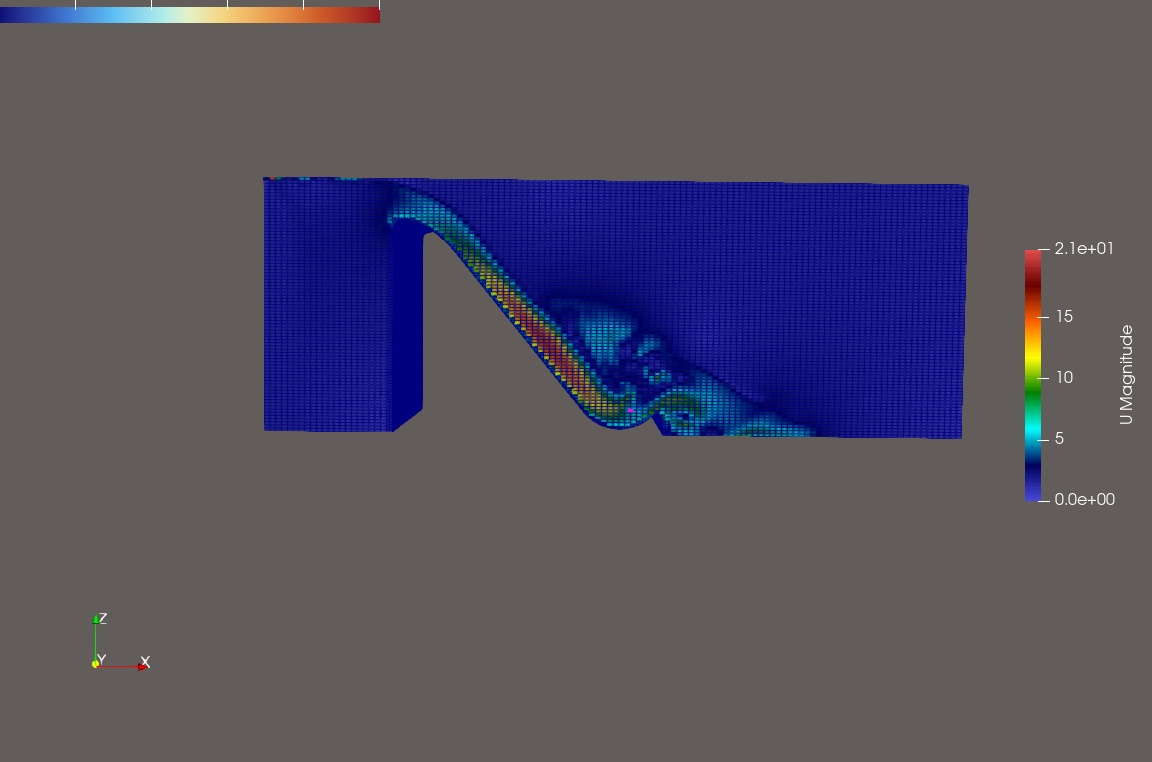
\includegraphics[width=\textwidth]{figures/ch9_q1051_U_profil.jpeg}
    \caption{Profil du champ de vitesse $\|\mathbf{U}\|$ (m/s) le long de l'évacuateur de crues — simulation exploratoire $Q = 1\,051$ m³/s. Les vitesses sur le coursier atteignent jusqu'à $21$ m/s et l'écoulement à la cuillère présente un caractère fortement turbulent avec des structures tourbillonnaires visibles.}
    \label{fig:q1051_U_profil}
\end{figure}

Le profil de vitesse révèle une accélération continue de l'écoulement depuis la retenue (vitesses quasiment nulles, zone bleue) jusqu'à la cuillère, où les valeurs de $\|\mathbf{U}\|$ atteignent localement \textbf{21 m/s}, valeur maximale observée sur l'ensemble des simulations réalisées dans ce projet. La zone de la cuillère présente une structure nettement plus chaotique que pour les débits de projet ($Q_{10}$ à $Q_{1\,000}$) : les tourbillons et le décollement de lame visibles en sortie de cuillère signalent que l'ouvrage actuel fonctionne en dehors de ses conditions hydrauliques nominales, ce qui est attendu pour un débit excédant de plus de 32\,\% le débit de dimensionnement.

\begin{figure}[H]
    \centering
    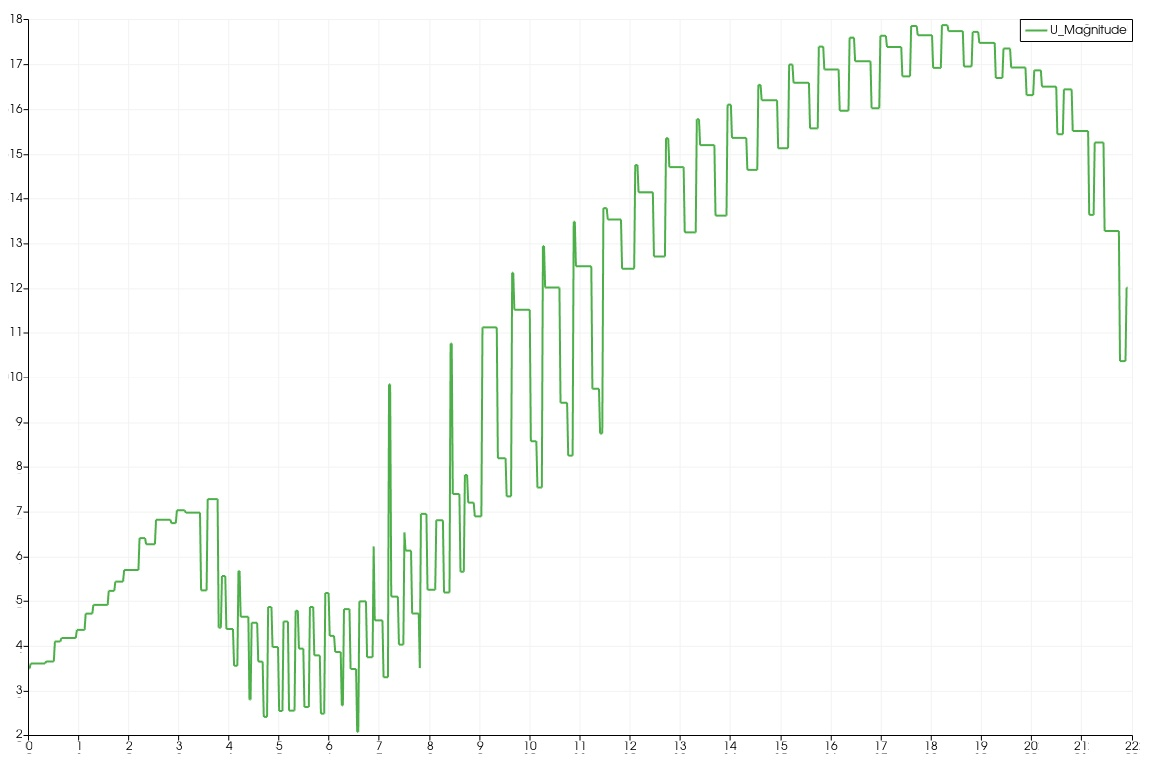
\includegraphics[width=\textwidth]{figures/ch9_q1051_U_graphe.jpeg}
    \caption{Évolution de la vitesse $\|\mathbf{U}\|$ (m/s) le long de l'axe longitudinal de l'évacuateur — simulation exploratoire $Q = 1\,051$ m³/s. La vitesse augmente progressivement de $\approx 3{,}5$ m/s en entrée jusqu'à $\approx 17{,}5$ m/s au niveau de la cuillère, avant une chute brusque liée au décollement en sortie.}
    \label{fig:q1051_U_graphe}
\end{figure}

Le graphe d'évolution de la vitesse confirme la tendance générale observée sur le profil. On distingue plusieurs phases :
\begin{itemize}
    \item \textbf{Zone 0–3 m} : montée progressive de la vitesse ($3{,}5$ à $7$ m/s) correspondant à l'approche et au déversement sur le seuil Creager ;
    \item \textbf{Zone 3–7 m} : oscillations marquées ($2{,}5$ à $7$ m/s) traduisant la zone de transition turbulente en aval immédiat du seuil, avec des gradients de phase air/eau intenses ;
    \item \textbf{Zone 8–17 m} : montée quasi-monotone de la vitesse ($8$ à $18$ m/s), caractéristique d'un écoulement supercritique bien établi sur le coursier incliné ;
    \item \textbf{Zone 17–22 m} : légère décroissance ($18$ à $10{,}5$ m/s) en fin de cuillère, correspondant au décollement de la lame et à la formation du jet aérien.
\end{itemize}

Ces valeurs, significativement plus élevées que celles obtenues pour $Q_{1\,000}$, confirment la forte sollicitation hydraulique de l'ouvrage dans ce scénario exploratoire.

\subsection{Champ de pression}
\label{subsec:q1051_pression}

\begin{figure}[H]
    \centering
    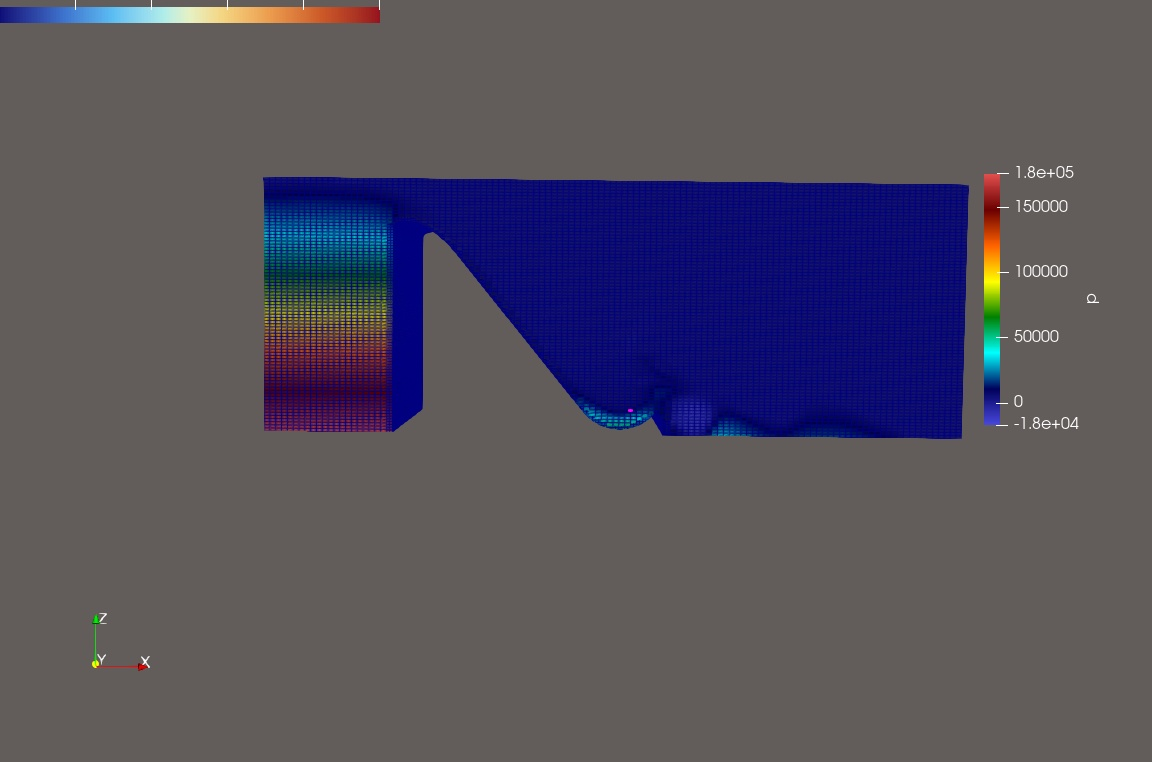
\includegraphics[width=\textwidth]{figures/ch9_q1051_P_profil.jpeg}
    \caption{Profil du champ de pression $p$ (Pa) le long de l'évacuateur de crues — simulation exploratoire $Q = 1\,051$ m³/s. La retenue amont présente une pression hydrostatique maximale atteignant $1{,}8 \times 10^5$ Pa. Deux zones de sous-pression (pression légèrement négative) sont visibles à la base de la cuillère, signalant un risque potentiel de cavitation.}
    \label{fig:q1051_P_profil}
\end{figure}

La distribution de pression pour $Q = 1\,051$ m³/s met en évidence deux éléments particulièrement importants :

\begin{itemize}
    \item \textbf{Pression hydrostatique dans la retenue} : la retenue amont présente un gradient de pression hydrostatique marqué, avec des valeurs allant de $0$ Pa en surface jusqu'à environ $1{,}8 \times 10^5$ Pa au pied du barrage. Ce gradient, plus intense qu'aux débits de projet, traduit la charge hydraulique élevée exercée sur l'ouvrage dans ce scénario.
    \item \textbf{Zones de sous-pression à la cuillère} : deux poches de pression légèrement négative (teinte cyan, $p \approx -18\,000$ Pa) sont clairement identifiables au niveau de la base de la cuillère saut de ski. Ces dépressions sont la conséquence directe de la forte courbure convexe et des vitesses très élevées (${\sim}\,20$ m/s) : selon l'équation de Bernoulli, la pression est inversement corrélée au carré de la vitesse dans les zones de courbure. Ce phénomène, s'il s'intensifie, peut conduire à de la \textbf{cavitation}, mécanisme susceptible d'engendrer des dégradations par érosion des parois en béton.
\end{itemize}

\begin{figure}[H]
    \centering
    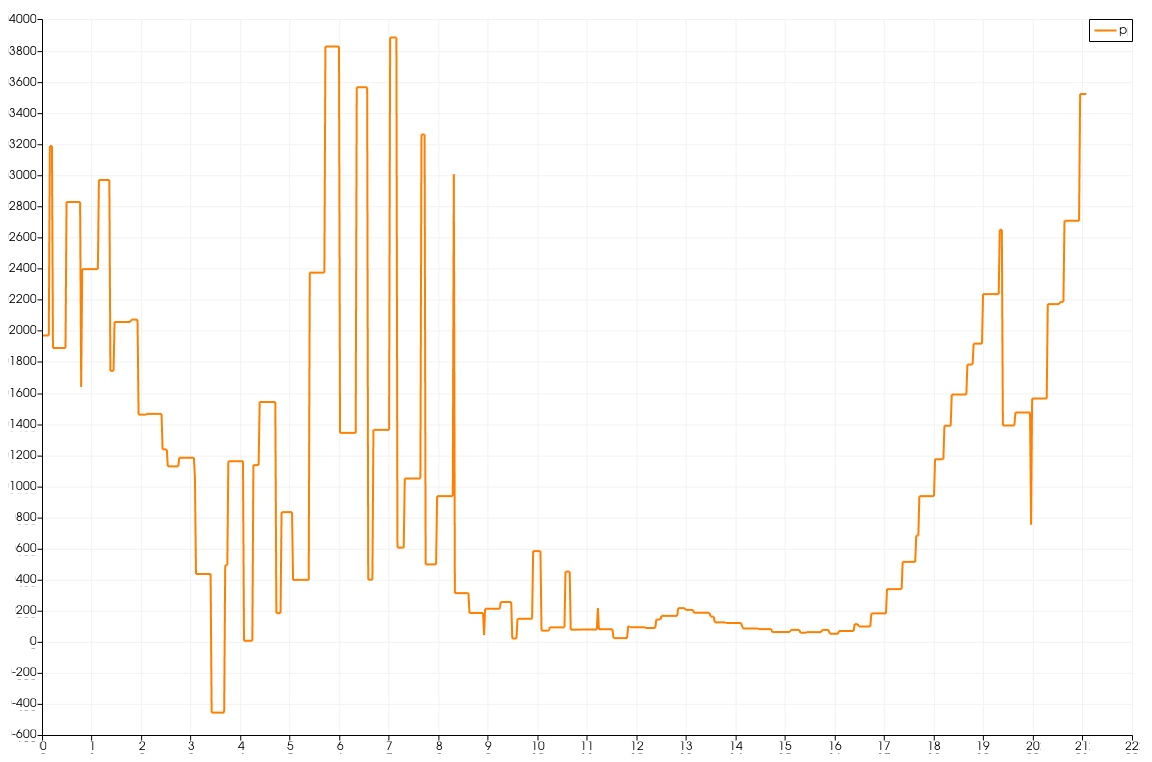
\includegraphics[width=\textwidth]{figures/ch9_q1051_P_graphe.jpeg}
    \caption{Évolution de la pression $p$ (Pa) le long de l'axe longitudinal de l'évacuateur — simulation exploratoire $Q = 1\,051$ m³/s. La pression chute à des valeurs proches de zéro sur le coursier torrentiel (x\,=\,8--17 m), avant de remonter à la cuillère. Les oscillations dans la zone du seuil (x\,=\,3--8 m) reflètent la turbulence de la transition de régime.}
    \label{fig:q1051_P_graphe}
\end{figure}

Le graphe de pression illustre l'évolution longitudinale suivante :
\begin{itemize}
    \item \textbf{x = 0–3 m} : pression de $1\,800$ à $3\,200$ Pa, représentant la charge piézométrique de la lame déversante au-dessus du seuil Creager ;
    \item \textbf{x = 3–8 m} : zone fortement oscillante avec des pics dépassant $3\,800$ Pa et une dépression à $-400$ Pa — reflet de la turbulence intense lors de la transition fluvial/torrentiel et du passage de la vague sur la crête du seuil ;
    \item \textbf{x = 8–17 m} : pression quasi nulle ($50$–$600$ Pa), confirmant un régime supercritique établi : la lame d'eau très mince et rapide n'exerce qu'une pression négligeable sur le radier ;
    \item \textbf{x = 17–22 m} : remontée progressive de la pression ($1\,500$ à $3\,500$ Pa), correspondant à la courbure ascendante de la cuillère qui dévie le jet vers le haut et génère une surpression centrifuge sur le radier de la cuillère.
\end{itemize}

\subsection{Charge sur le seuil ($H_d$)}
\label{subsec:q1051_hd}

\begin{figure}[H]
    \centering
    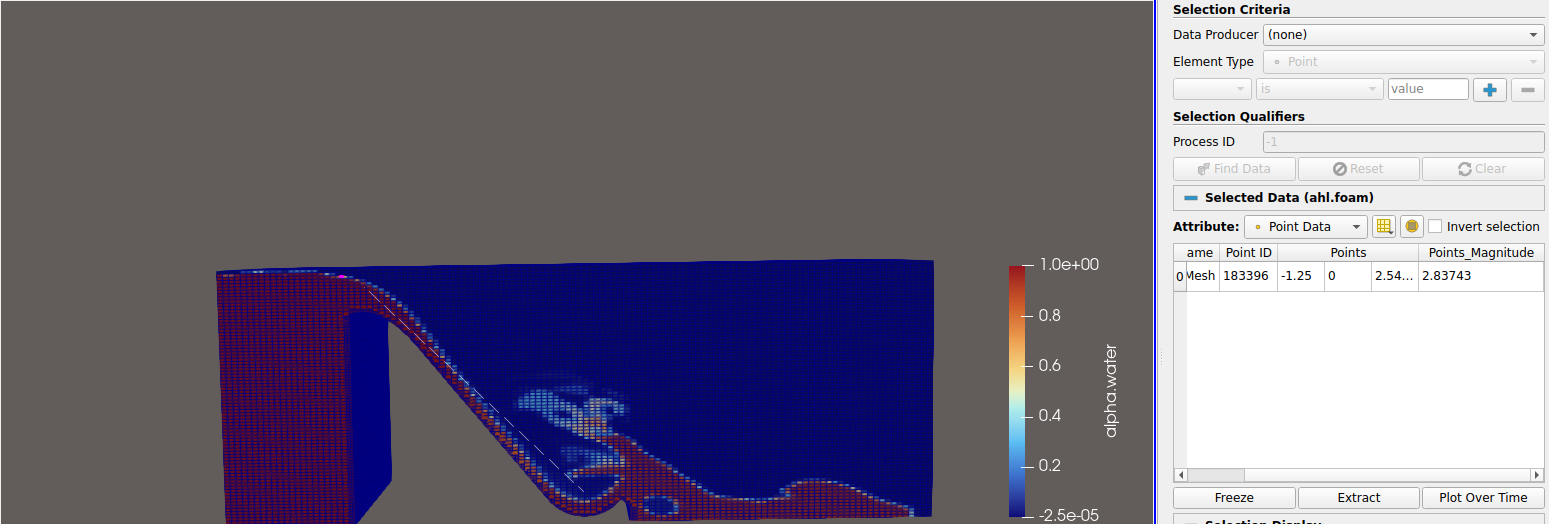
\includegraphics[width=\textwidth]{figures/ch9_q1051_Hd.png}
    \caption{Hauteur d'eau au seuil Creager — simulation exploratoire $Q = 1\,051$ m³/s. La charge simulée sur le seuil, lue directement depuis la coordonnée Z du point de surface libre sélectionné dans le tableau de données ParaView, est $H_d \approx 2{,}54$ m.}
    \label{fig:q1051_Hd}
\end{figure}

La charge simulée sur le seuil pour $Q = 1\,051$ m³/s est $H_d \approx 2{,}54$ m, lue directement sur la coordonnée verticale $z$ du point de surface libre sélectionné dans le panneau \textit{Selected Data} de ParaView. Cette valeur, identique à celle mesurée pour le débit millénal $Q_{1\,000} = 794{,}93$ m³/s, mérite une interprétation nuancée : d'une part, la surcharge hydraulique exercée par le débit supplémentaire ($\Delta Q \approx 256$ m³/s) ne se traduit pas nécessairement par une hausse proportionnelle de la charge au seuil, car la largeur déversante et la géométrie du profil Creager permettent d'absorber une partie de l'augmentation par une légère extension de la lame déversante en largeur ; d'autre part, la mesure exploratoire sur un point unique de la surface libre présente une incertitude inhérente à la rugosité numérique de l'interface air-eau dans un écoulement aussi turbulent. À titre comparatif, la théorie de la loi débit-charge ($Q = C_d \cdot L \cdot H_d^{3/2}$) prévoit une charge théorique de l'ordre de $H_d^{\text{th}} \approx 3{,}05$ m pour ce débit, ce qui suggère que la valeur lue sous-estime légèrement la charge réelle du fait du point de mesure.

\subsection{Observations générales et recommandations}
\label{subsec:q1051_discussion}

L'ensemble des résultats de cette simulation exploratoire conduit aux observations suivantes :

\begin{enumerate}
    \item \textbf{Fonctionnement hors plage nominale} : à $Q = 1\,051$ m³/s, l'évacuateur de crues actuel fonctionne nettement au-delà de ses conditions de dimensionnement. Les vitesses maximales (jusqu'à $21$ m/s), les structures tourbillonnaires à la cuillère et les zones de sous-pression attestent d'une sollicitation hydraulique extrême.

    \item \textbf{Risque de cavitation à la cuillère} : les zones de pression négative identifiées à la base de la cuillère ($p \approx -18\,000$ Pa) constituent un signal d'alerte important. Pour une pression de vapeur saturante de l'eau à $20°$C d'environ $2\,300$ Pa en pression absolue, et une pression atmosphérique de $101\,325$ Pa, la pression absolue au niveau de ces zones resterait positive (environ $83\,000$ Pa), ce qui situe le phénomène en dessous du seuil de cavitation proprement dit. Cependant, la dynamique réelle de l'écoulement, avec des fluctuations turbulentes non représentées par le modèle RANS, pourrait localement abaisser la pression instantanée en dessous du seuil de vaporisation. Une étude complémentaire par simulation LES (Large Eddy Simulation) serait nécessaire pour trancher définitivement.

    \item \textbf{Pertinence de la surélévation envisagée} : ces résultats confirment qu'une surélévation du barrage devra impérativement s'accompagner d'une révision complète du profil hydraulique de l'évacuateur de crues : seuil Creager redimensionné, coursier adapté en section et en pente, et cuillère recalculée pour les nouvelles conditions d'éjection. L'utilisation d'OpenFOAM dans le cadre de la présente étude a montré sa capacité à identifier avec précision les zones sensibles et à guider les choix de conception.

    \item \textbf{Valeur indicative de la simulation} : malgré ses limites, cette simulation fournit un encadrement utile du comportement de l'ouvrage actuel et confirme que la géométrie de la cuillère saut de ski reste fonctionnelle pour des débits nettement supérieurs à $Q_{1\,000}$, ce qui témoigne d'une robustesse hydraulique appréciable de la conception initiale.
\end{enumerate}

% ============================================================
%  SECTION 9.6 : DISCUSSION
% ============================================================
\section{Discussion, limites de l'étude et recommandations}
\label{sec:discussion_limites_recommandations}

\subsection{Limites de l'étude}
\label{subsec:limites_etude}

Les résultats présentés dans ce chapitre doivent être interprétés en tenant compte des limites suivantes :
\begin{itemize}
    \item \textbf{Sensibilité au maillage} : les résultats correspondent au maillage retenu à l'issue de l'étude de sensibilité (section \ref{subsec:sensibilite_maillage}) ; un raffinement supplémentaire, notamment au niveau de l'interface air-eau et du jet, pourrait affiner certains résultats au prix d'un coût de calcul accru ;
    \item \textbf{Modèle de turbulence} : le modèle $k$-$\omega$ SST, de type RANS, repose sur une approche statistique de la turbulence et ne représente pas explicitement le transport des bulles d'air dans l'écoulement diphasique, ce qui peut limiter la précision de la représentation de l'aération sur le coursier et le jet ;
    \item \textbf{Hypothèse de régime quasi-permanent} : chaque débit de crue est simulé en régime permanent, sans représenter la dynamique de montée et de décrue de l'hydrogramme de crue ;
    \item \textbf{Simplifications géométriques} : le modèle géométrique, construit sous SketchUp à partir des profils types, peut ne pas intégrer certains détails constructifs mineurs de l'ouvrage réel ;
    \item \textbf{Étendue du domaine de calcul} : les conditions aux limites aval et latérales sont placées à une distance finie de l'ouvrage ; leur influence éventuelle sur la zone d'impact du jet et la fosse d'érosion doit être gardée à l'esprit.
\end{itemize}

\subsection{Recommandations}
\label{subsec:recommandations}

Sur la base des résultats obtenus, les recommandations suivantes peuvent être formulées :
\begin{itemize}
    \item \textbf{Suivi in situ} : il est recommandé de mettre en place une instrumentation de suivi permettant de comparer, lors d'un futur événement de crue, le comportement réel de l'ouvrage aux résultats de la présente étude ;
    \item \textbf{Vérification des murs bajoyers} : la hauteur des murs bajoyers retenue à la section \ref{sec:murs_bajoyers} doit être confrontée aux hauteurs d'eau maximales obtenues numériquement (figures \ref{fig:q10_h_coursier}, \ref{fig:q100_h_coursier} et \ref{fig:q1000_h_coursier}), en particulier pour $Q_{1\,000}$ ;
    \item \textbf{Protection contre l'affouillement} : en fonction des points d'impact obtenus numériquement (figures \ref{fig:q10_jet}, \ref{fig:q100_jet} et \ref{fig:q1000_jet}) et de la profondeur d'affouillement estimée (section \ref{sec:affouillement}), la nécessité d'une protection complémentaire du lit aval pourra être réévaluée ;
    \item \textbf{Études complémentaires} : un raffinement local du maillage au niveau de l'interface et du jet, ainsi qu'une simulation transitoire suivant l'hydrogramme complet de la crue de projet, permettraient d'affiner les conclusions de la présente étude.
\end{itemize}


% --- ANNEXES ---
\clearpage
\appendix
\addcontentsline{toc}{part}{ANNEXES}
% ============================================================
%  ANNEXES
% ============================================================

% ============================================================
%  ANNEXE 1 : SIMULATIONS HEC-RAS
% ============================================================
\chapter{Les simulations sur le Logiciel HEC-RAS pour le calcul de la lame d'eau sur le coursier}
\label{ann:hecras}

\section{Introduction}
\label{sec:ann1_intro}

La présente annexe regroupe les éléments détaillés de la modélisation unidimensionnelle réalisée sous le logiciel HEC-RAS (\textit{Hydrologic Engineering Center -- River Analysis System}) dans le cadre du dimensionnement hydraulique de l'évacuateur de crues du barrage Ahl Souss. Cette modélisation, dont les principes et les résultats synthétiques sont présentés à la section \ref{sec:murs_bajoyers} du chapitre \ref{chap:dim_theorique}, a pour objectif de déterminer le profil de la ligne d'eau le long du coursier pour les trois débits de crue retenus (périodes de retour 10, 100 et 1\,000 ans), afin d'en déduire la hauteur des murs bajoyers nécessaire à la contenance de l'écoulement.

\section{Mise en place du modèle HEC-RAS}
\label{sec:ann1_modele}

\subsection{Etapes de la détermination de la lame d'eau sur le coursier}
\label{subsec:ann1_geometrie}

La première étape pour les simulations, avant la création d'un nouveau projet, consiste à régler les unités sur le système international SI, et ce en faisant : « \textbf{Options -- Unit System -- System International} »

Puis, pour la création d'un nouveau projet, on suit le cheminement : « \textbf{File -- New project} » et on lui donne un titre après le choix de son emplacement.

L'option « \textbf{Geometric Data -- River Reach} » permet de dessiner la géométrie du coursier comme suit :

\begin{figure}[H]
    \centering
    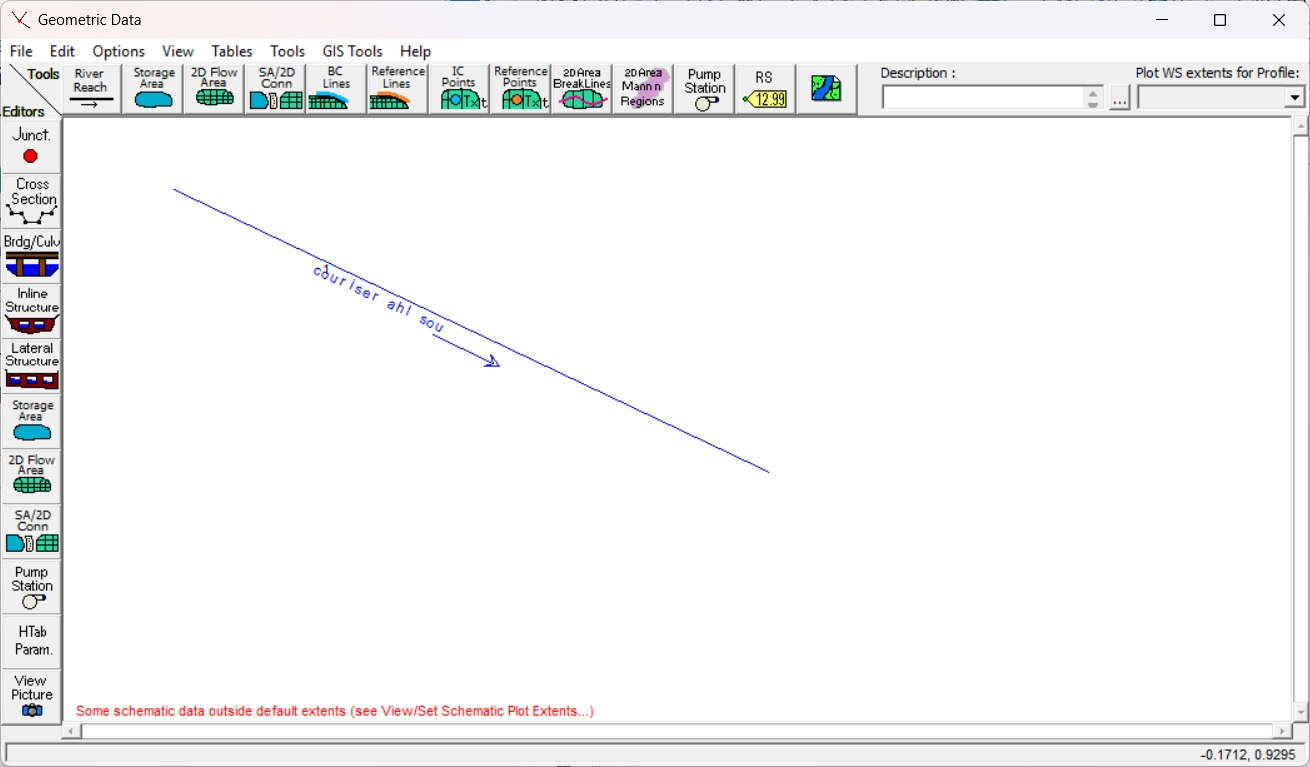
\includegraphics[width=0.85\textwidth]{figures/ann1_coursier_hecras.jpeg}
    \caption{Tracé schématique du coursier « coursier ahl sou » dans l'interface \textit{Geometric Data} de HEC-RAS (option \textit{River Reach})}
    \label{fig:ann1_coursier_hecras}
\end{figure}

L'étape suivante consiste à ajouter des sections transversales sur le coursier en cliquant sur « \textbf{Cross Section} » et on remplit les données concernant trois sections pour notre cas : section avale, section amont et la section de changement de la pente du coursier.

Les données à rentrer pour chaque section sont :
\begin{itemize}
    \item Les quatre coordonnées de la section (2 points niveau haut et 2 points niveau bas) ;
    \item La longueur séparant la section présente avec la section la plus proche en aval ;
    \item Les coefficients de Mannings prenant la valeur 0,014 pour le coursier construit en béton ;
    \item Les abscisses des stations rive gauche et rive droite ;
    \item Les coefficients d'expansion (0,3) et de contraction (0,1).
\end{itemize}

A noter que le logiciel commence toujours les sections de l'aval vers l'amont.

\begin{figure}[H]
    \centering
    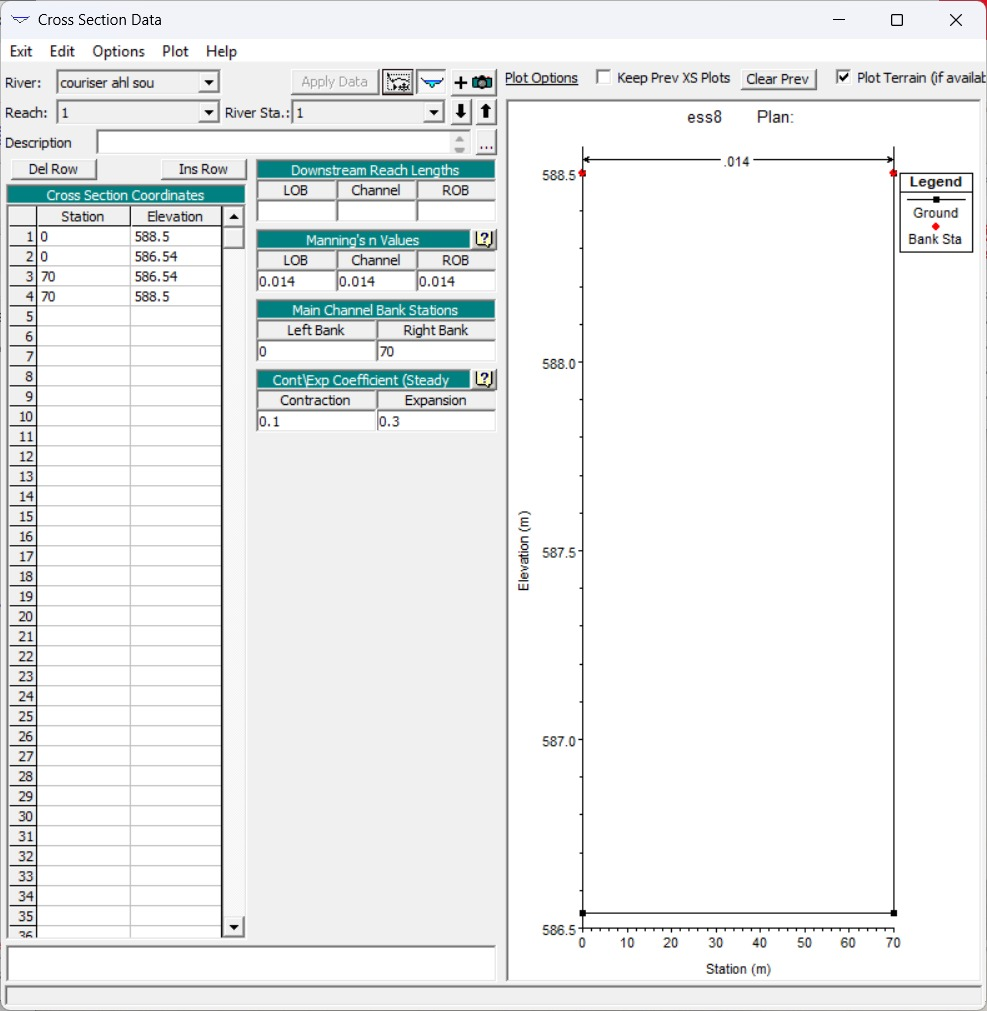
\includegraphics[width=\textwidth,height=0.42\textheight,keepaspectratio]{figures/ann1_section_aval.jpeg}\\[0.5em]
    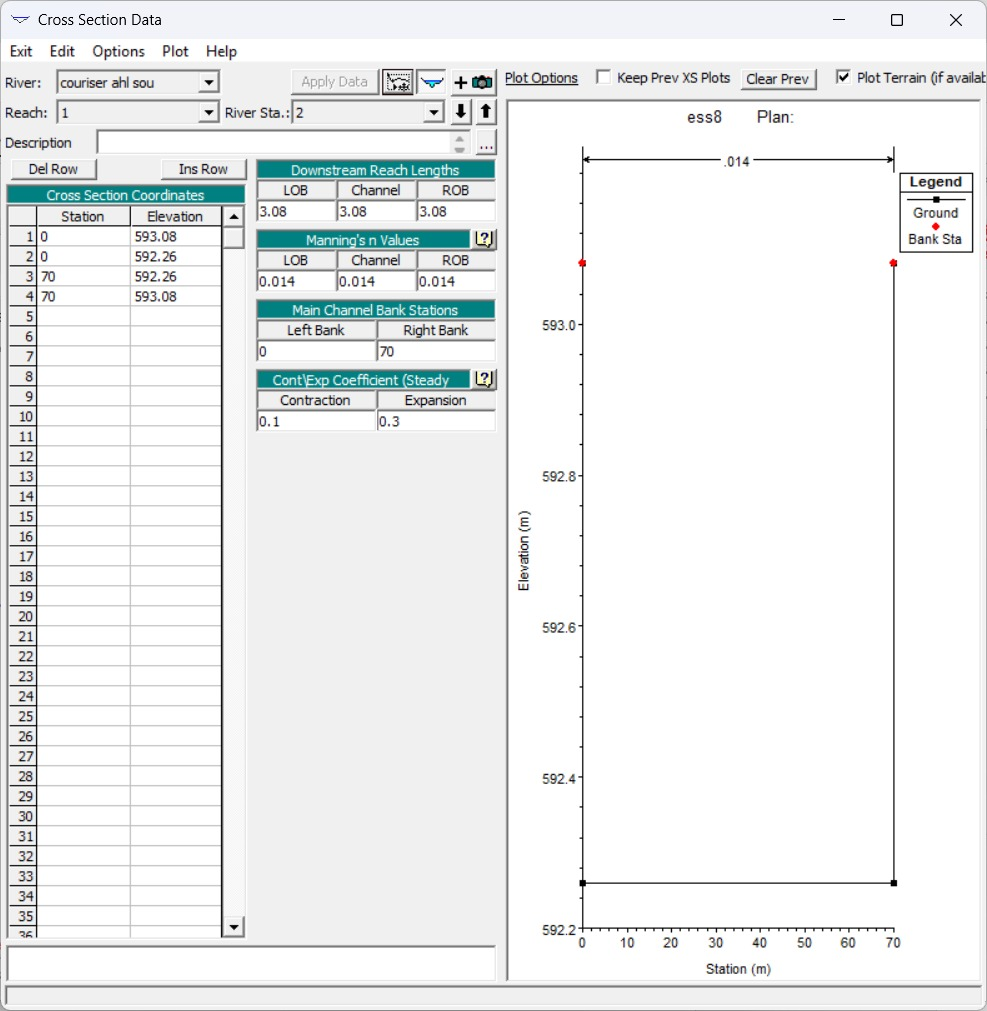
\includegraphics[width=\textwidth,height=0.42\textheight,keepaspectratio]{figures/ann1_section_changement_pente.jpeg}
\end{figure}

\clearpage

\begin{figure}[H]
    \centering
    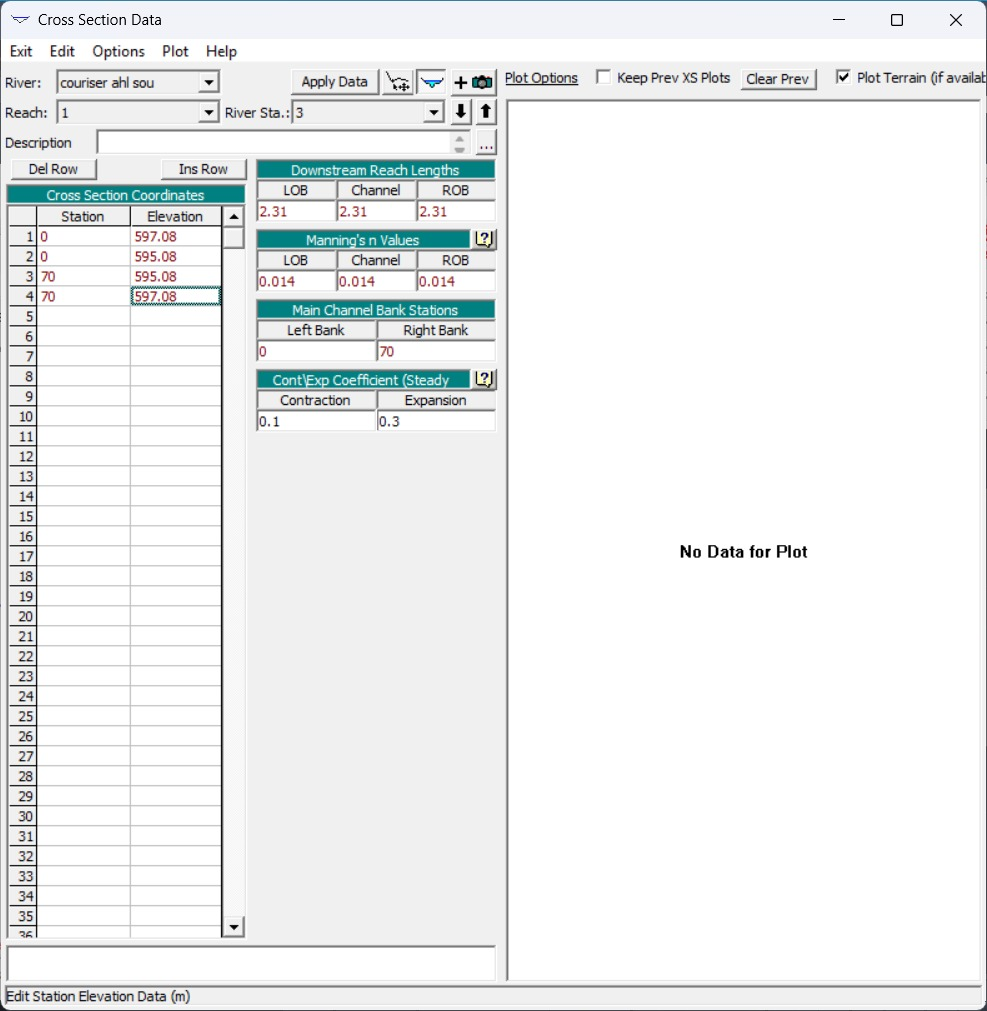
\includegraphics[width=\textwidth,height=0.75\textheight,keepaspectratio]{figures/ann1_section_amont.jpeg}
    \caption{Saisie des données des trois sections transversales du coursier dans HEC-RAS : section aval (RS\,=\,1), section de changement de pente (RS\,=\,2) et section amont (RS\,=\,3)}
    \label{fig:ann1_sections_transversales}
\end{figure}

Une fois que les données de chaque section sont remplies, on les conserve par « \textbf{Apply Data} ».

Pour ajouter d'autres sections transversales, afin de caractériser l'écoulement sur presque tout le coursier, on fait l'interpolation entre les sections pré-dessinées avec un pas de $2\,m$ en suivant « \textbf{Geometric Data -- Tools -- XS Interpolation} » :

\begin{figure}[H]
    \centering
    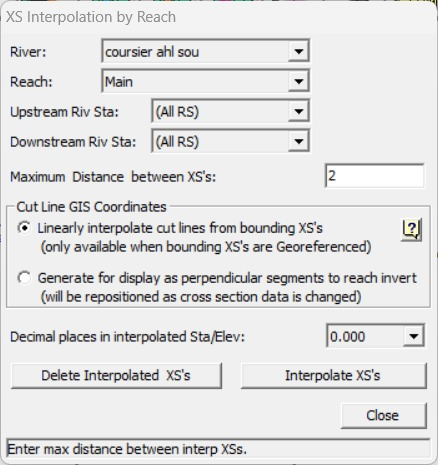
\includegraphics[width=0.65\textwidth]{figures/ann1_xs_interpolation.jpeg}
    \caption{Boîte de dialogue \textit{XS Interpolation by Reach} — interpolation des sections transversales avec un pas de 2\,m}
    \label{fig:ann1_xs_interpolation}
\end{figure}

Le résultat de l'interpolation est illustré par la figure suivante :

\begin{figure}[H]
    \centering
    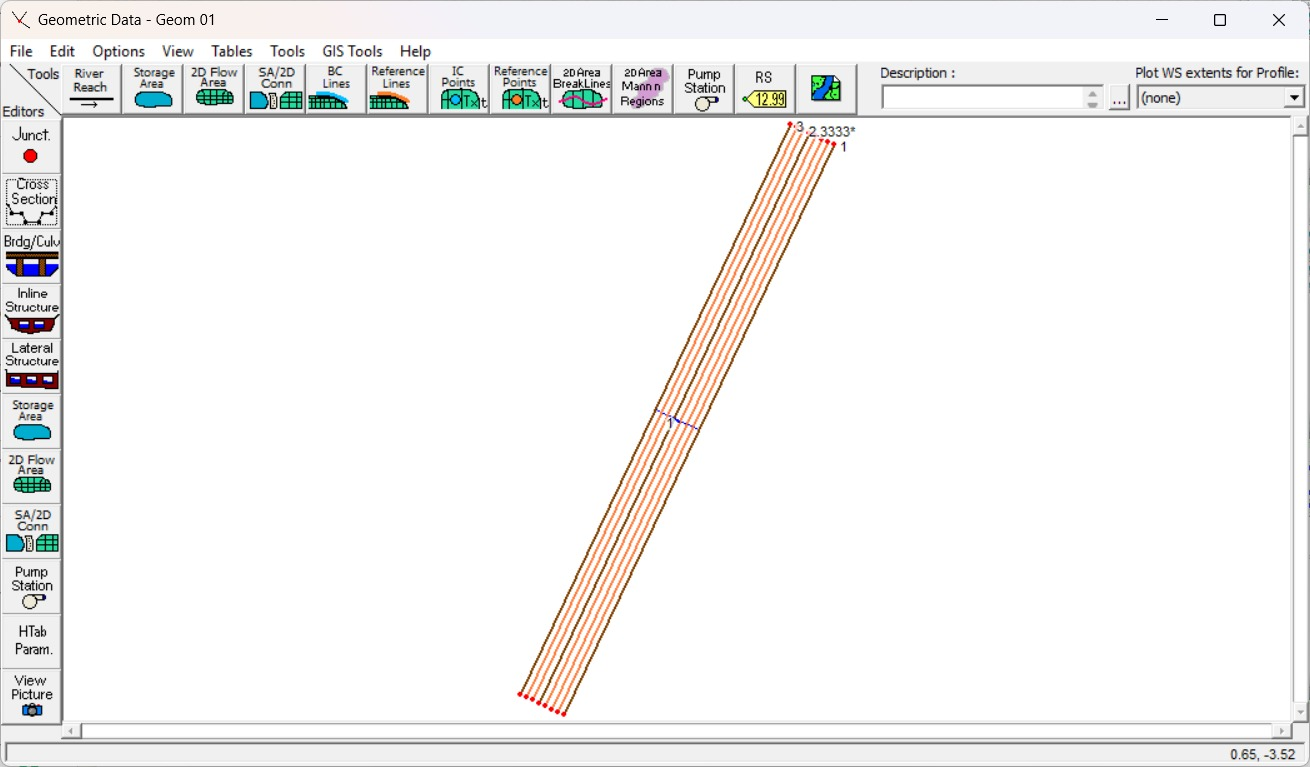
\includegraphics[width=0.85\textwidth]{figures/ann1_resultat_interpolation.jpeg}
    \caption{Visualisation des sections interpolées sur le coursier dans HEC-RAS}
    \label{fig:ann1_sections_interpolees}
\end{figure}

L'étape suivante consiste à entrer le débit de projet au logiciel et lui fixer les conditions aux limites.

Le débit de projet est inséré dans « \textbf{Steady Flow Data} » :

\begin{figure}[H]
    \centering
    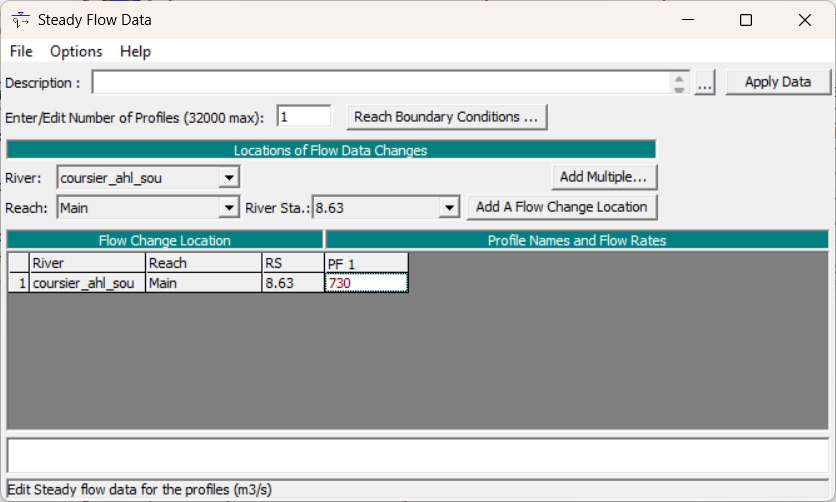
\includegraphics[width=0.85\textwidth]{figures/ann1_steady_flow_data.jpeg}
    \caption{Insertion du débit de projet et des conditions aux limites dans HEC-RAS (\textit{Steady Flow Data})}
    \label{fig:ann1_steady_flow}
\end{figure}

Les conditions aux limites sont insérées dans « \textbf{Steady Flow Data -- Reach Boundary Conditions} » en considérant la profondeur critique comme condition amont et la pente 18\,\% comme condition avale :

\begin{figure}[H]
    \centering
    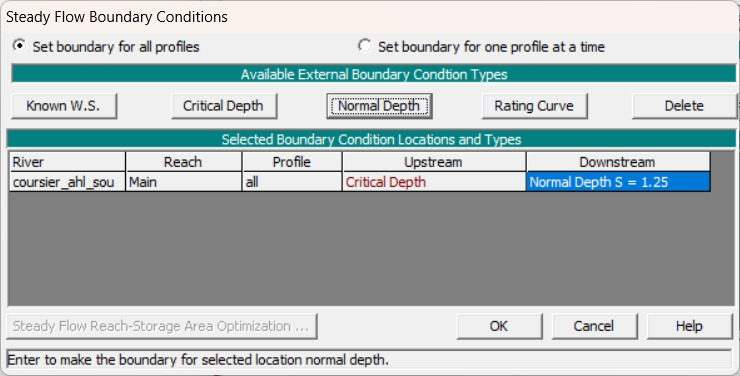
\includegraphics[width=0.85\textwidth]{figures/ann1_boundary_conditions.jpeg}
    \caption{Choix des conditions aux limites dans \textit{Steady Flow Boundary Conditions} : profondeur critique en amont, pente normale ($S = 1{,}25$) en aval}
    \label{fig:ann1_boundary_conditions}
\end{figure}

La dernière étape concerne l'exécution de la simulation qui consiste à fixer le régime de l'écoulement (fluvial ou torrentiel) et ce à travers « \textbf{Steady Flow Analysis} ». HEC-RAS donne la possibilité de le laisser lui-même déterminer le régime de l'écoulement en le fixant sur « \textbf{Mixed} ». L'exécution de la simulation se fait par « \textbf{Compute} » :

\begin{figure}[H]
    \centering
    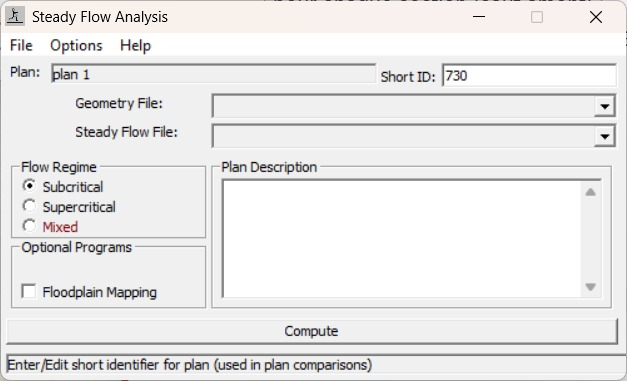
\includegraphics[width=0.75\textwidth]{figures/ann1_steady_flow_analysis.jpeg}
    \caption{Exécution de la simulation du projet HEC-RAS (\textit{Steady Flow Analysis}, régime Mixed)}
    \label{fig:ann1_steady_flow_analysis}
\end{figure}

Après quelques secondes, la simulation s'effectue avec réussite. Dès lors les résultats (Courbes, Dessins 2D, Tableaux\ldots) sont disponibles à visualiser.

\begin{figure}[H]
    \centering
    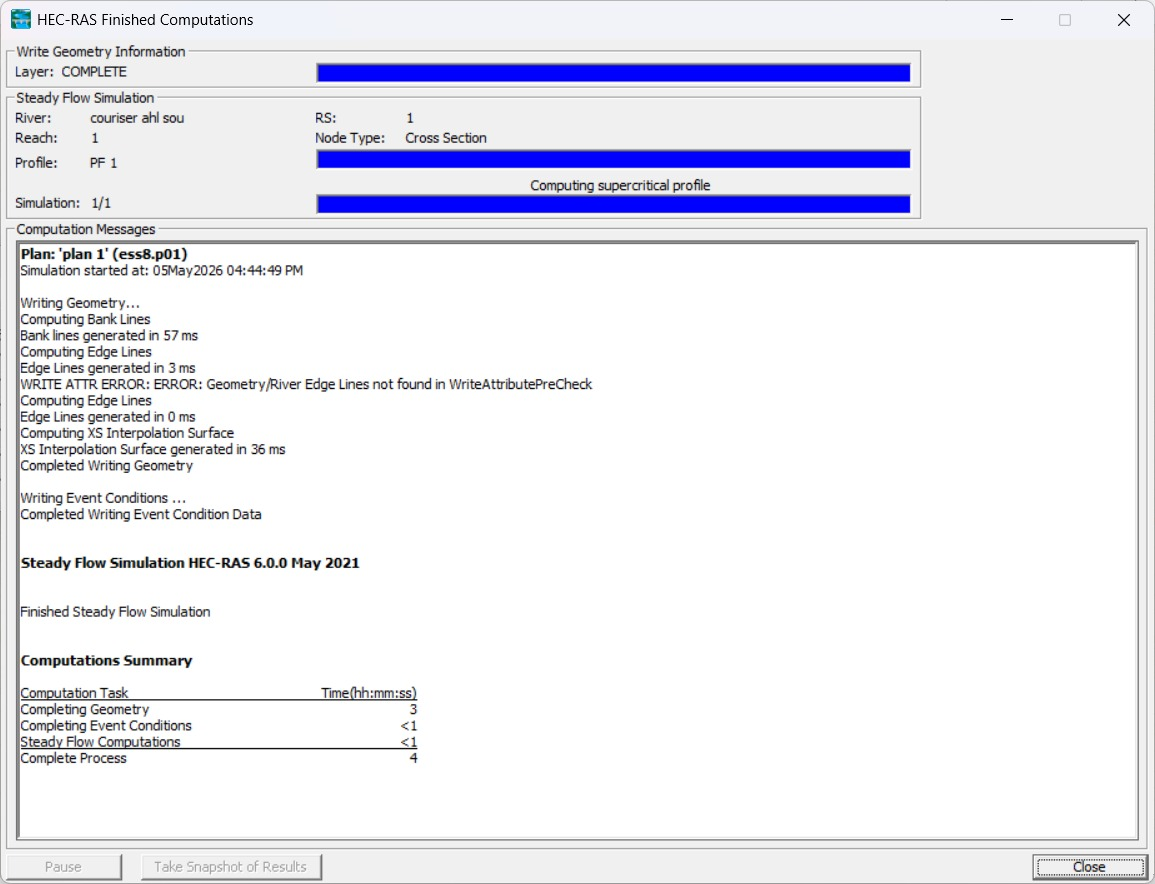
\includegraphics[width=0.92\textwidth]{figures/ann1_fin_simulation.jpeg}
    \caption{Interface de la fin de la simulation HEC-RAS (\textit{HEC-RAS Finished Computations})}
    \label{fig:ann1_finished_computations}
\end{figure}

% ============================================================
%  ANNEXE 2 : TABLEAUX DE CALCUL ET COURBES DE REMOUS
% ============================================================
\chapter{Les tableaux de calcul de la lame d'eau et les courbes de remous}
\label{ann:remous}

La présente annexe regroupe les tableaux complets de calcul de la courbe de remous établis par la méthode des pas dans le tableur Excel, pour chacun des trois débits de projet retenus ($Q_{10}$, $Q_{100}$ et $Q_{1\,000}$). Pour le débit millénaire $Q_{1\,000}$, le profil de la ligne d'eau est également représenté graphiquement.

% --- Q10 ---
\section{Tableau de calcul de la courbe de remous --- $Q_{10} = 175{,}11$ m³/s}
\label{sec:ann2_remous_q10}

\begin{figure}[H]
    \centering
    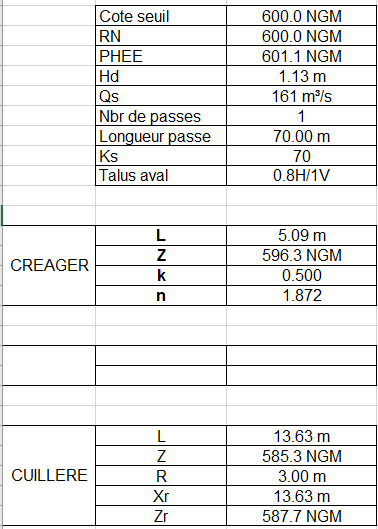
\includegraphics[width=0.65\textwidth]{figures/ann2_params_q10.png}
    \caption{Paramètres généraux de calcul pour $Q_{10} = 175{,}11$ m³/s : caractéristiques du seuil Creager et de la cuillère saut de ski}
    \label{fig:ann2_params_q10}
\end{figure}

\begin{figure}[H]
    \centering
    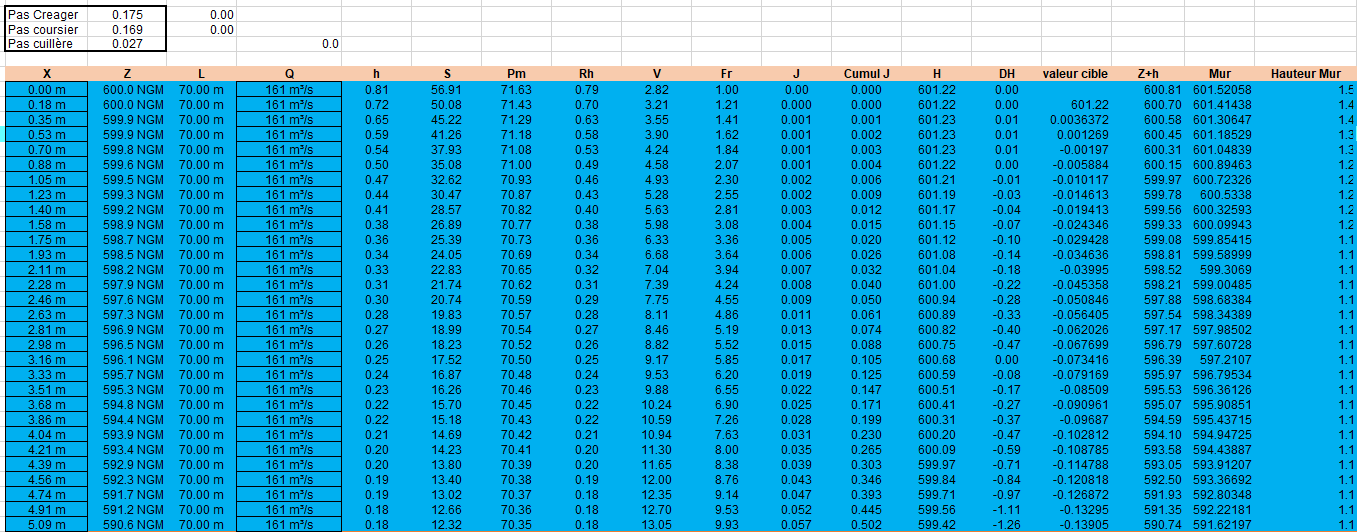
\includegraphics[width=\textwidth]{figures/ann2_seuil_q10.png}
    \caption{Tableau de calcul de la lame d'eau sur le seuil Creager — débit décennal $Q_{10} = 161$ m³/s (pas Creager\,=\,0,175\,m, pas coursier\,=\,0,169\,m, pas cuillère\,=\,0,027\,m)}
    \label{fig:ann2_seuil_q10}
\end{figure}

\begin{figure}[H]
    \centering
    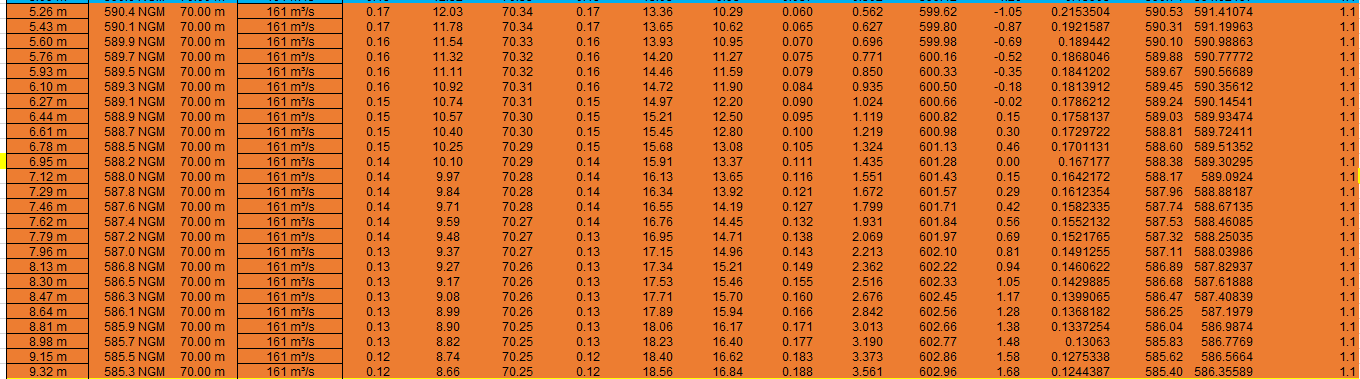
\includegraphics[width=\textwidth]{figures/ann2_coursier_q10.png}
    \caption{Tableau de calcul de la lame d'eau sur le coursier — débit décennal $Q_{10} = 161$ m³/s}
    \label{fig:ann2_coursier_q10}
\end{figure}

\begin{figure}[H]
    \centering
    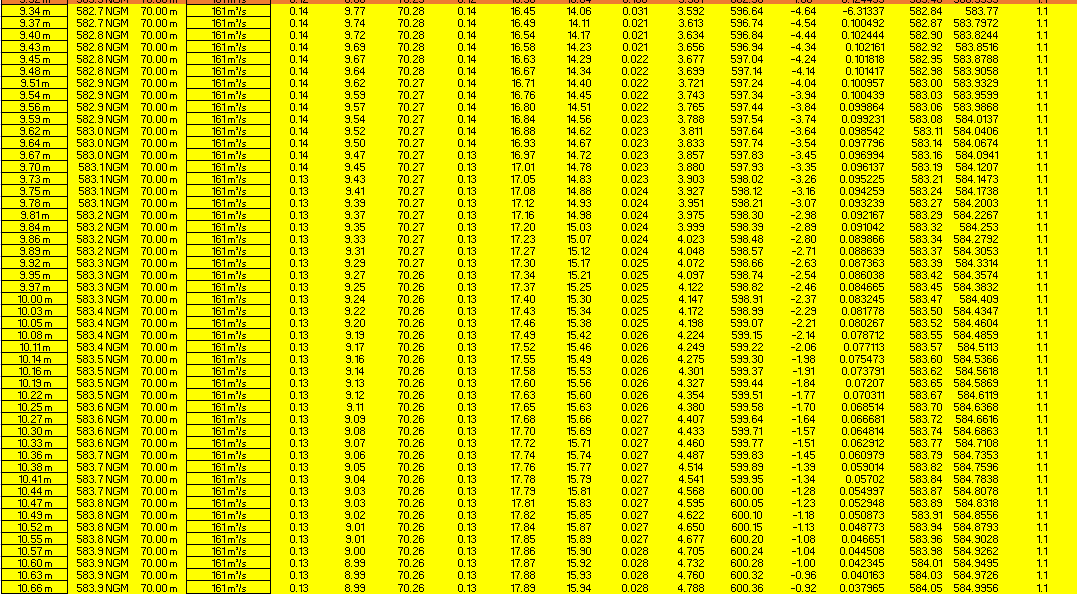
\includegraphics[width=\textwidth]{figures/ann2_cuillere_q10.png}
    \caption{Tableau de calcul de la lame d'eau sur la cuillère saut de ski — débit décennal $Q_{10} = 161$ m³/s}
    \label{fig:ann2_cuillere_q10}
\end{figure}

% --- Q100 ---
\section{Tableau de calcul de la courbe de remous --- $Q_{100} = 507{,}54$ m³/s}
\label{sec:ann2_remous_q100}

\begin{figure}[H]
    \centering
    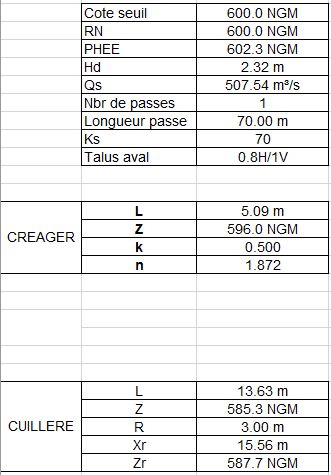
\includegraphics[width=0.65\textwidth]{figures/ann2_params_q100.png}
    \caption{Paramètres généraux de calcul pour $Q_{100} = 507{,}54$ m³/s : caractéristiques du seuil Creager et de la cuillère saut de ski}
    \label{fig:ann2_params_q100}
\end{figure}

\begin{figure}[H]
    \centering
    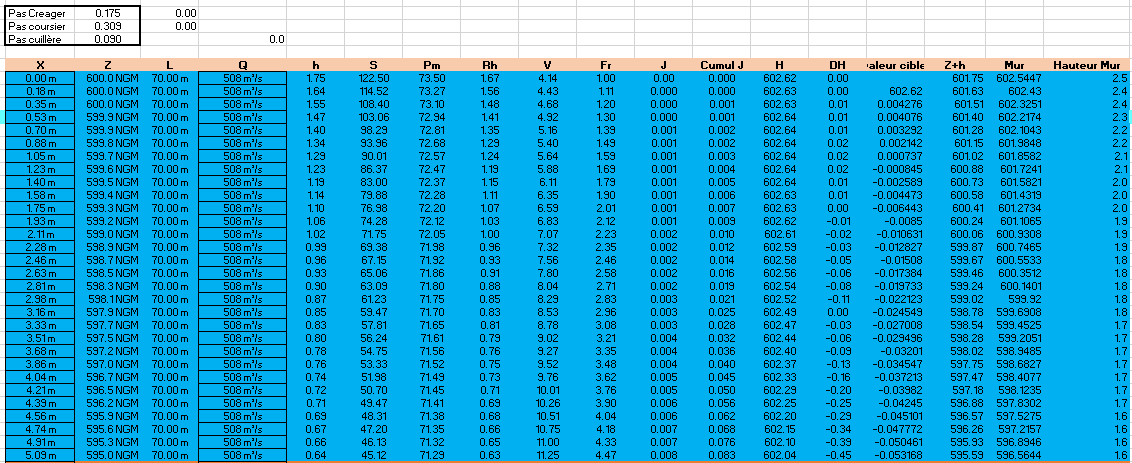
\includegraphics[width=\textwidth]{figures/ann2_seuil_q100.png}
    \caption{Tableau de calcul de la lame d'eau sur le seuil Creager — débit centennal $Q_{100} = 507{,}54$ m³/s}
    \label{fig:ann2_seuil_q100}
\end{figure}

\begin{figure}[H]
    \centering
    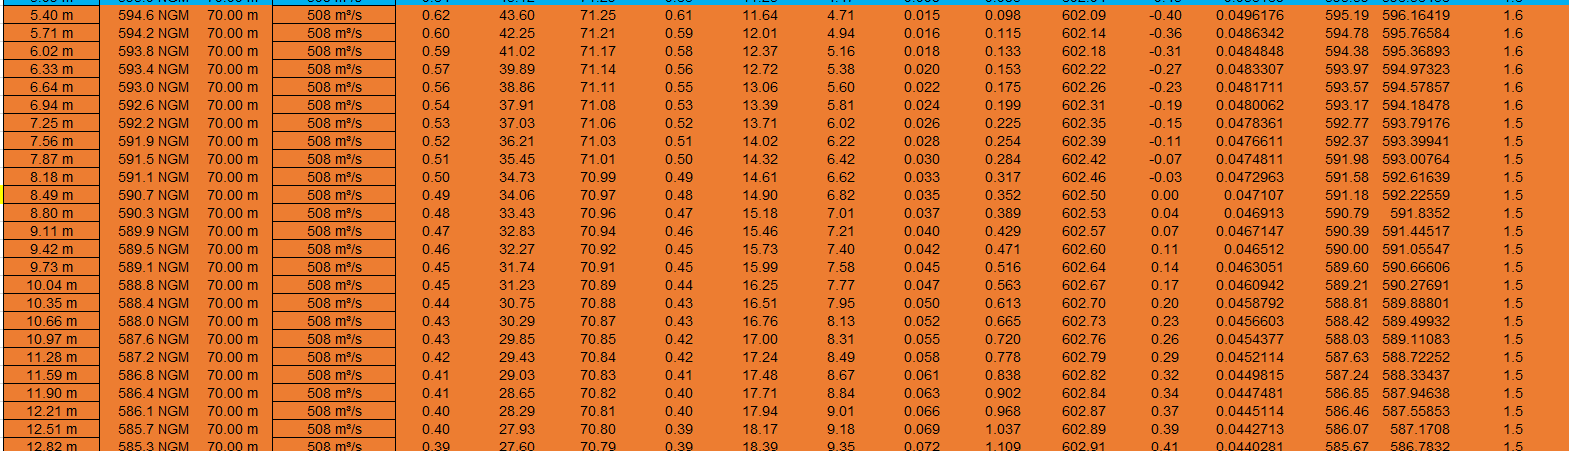
\includegraphics[width=\textwidth]{figures/ann2_coursier_q100.png}
    \caption{Tableau de calcul de la lame d'eau sur le coursier — débit centennal $Q_{100} = 507{,}54$ m³/s}
    \label{fig:ann2_coursier_q100}
\end{figure}

\begin{figure}[H]
    \centering
    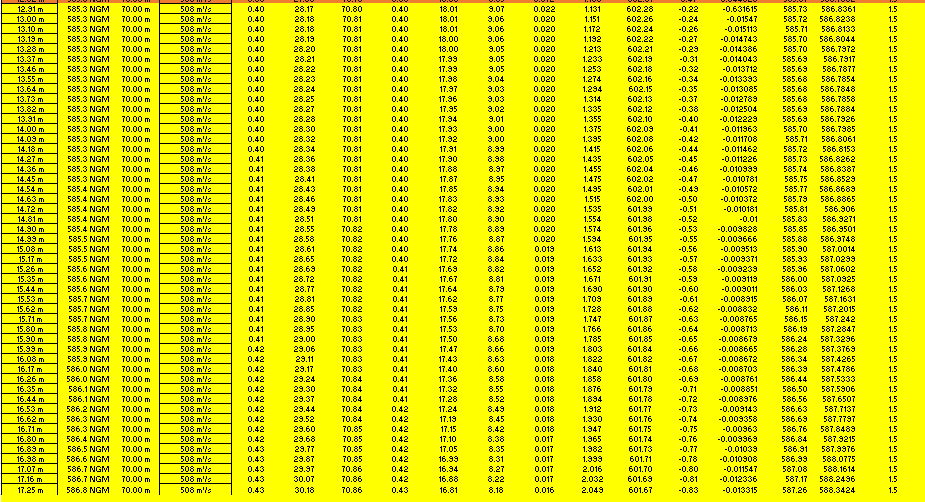
\includegraphics[width=\textwidth]{figures/ann2_cuillere_q100.png}
    \caption{Tableau de calcul de la lame d'eau sur la cuillère saut de ski — débit centennal $Q_{100} = 507{,}54$ m³/s}
    \label{fig:ann2_cuillere_q100}
\end{figure}

% --- Q1000 ---
\section{Tableau de calcul de la courbe de remous et graphe --- $Q_{1\,000} = 794{,}93$ m³/s}
\label{sec:ann2_remous_q1000}

\begin{figure}[H]
    \centering
    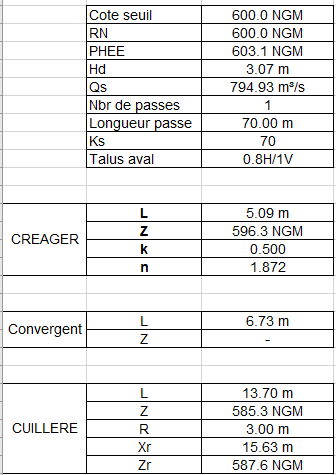
\includegraphics[width=0.65\textwidth]{figures/ann2_params_q1000.png}
    \caption{Paramètres généraux de calcul pour $Q_{1\,000} = 794{,}93$ m³/s : caractéristiques du seuil Creager et de la cuillère saut de ski}
    \label{fig:ann2_params_q1000}
\end{figure}

\begin{figure}[H]
    \centering
    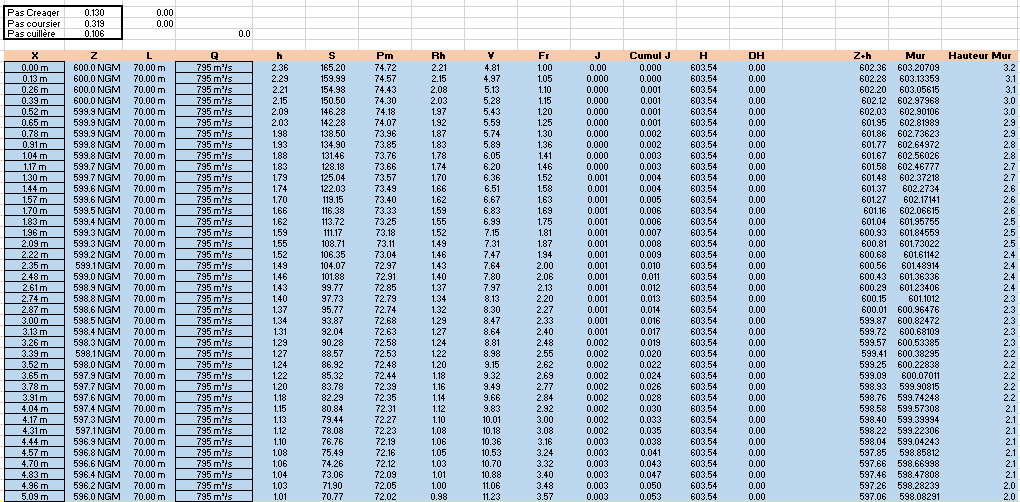
\includegraphics[width=\textwidth]{figures/ann2_seuil_q1000.png}
    \caption{Tableau de calcul de la lame d'eau sur le seuil Creager — débit millénaire $Q_{1\,000} = 794{,}93$ m³/s}
    \label{fig:ann2_seuil_q1000}
\end{figure}

\begin{figure}[H]
    \centering
    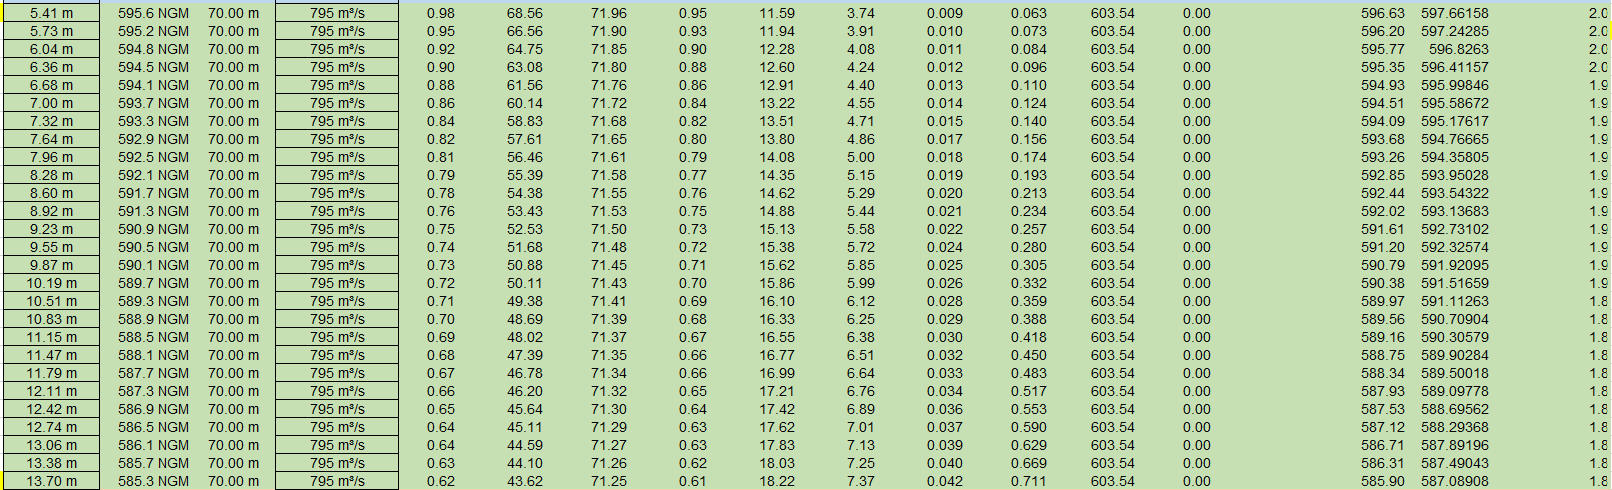
\includegraphics[width=\textwidth]{figures/ann2_coursier_q1000.png}
    \caption{Tableau de calcul de la lame d'eau sur le coursier — débit millénaire $Q_{1\,000} = 794{,}93$ m³/s}
    \label{fig:ann2_coursier_q1000}
\end{figure}

\begin{figure}[H]
    \centering
    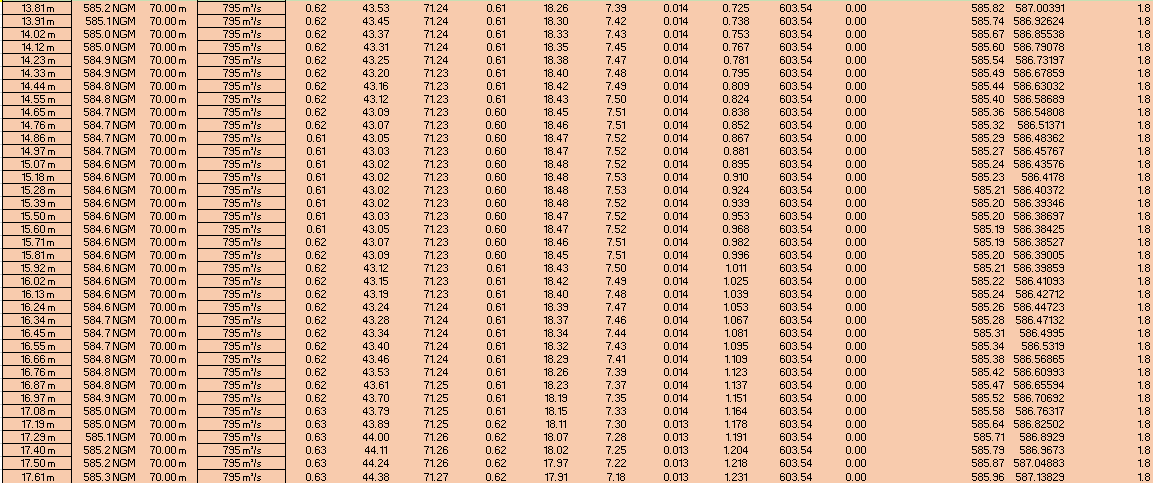
\includegraphics[width=\textwidth]{figures/ann2_cuillere_q1000.png}
    \caption{Tableau de calcul de la lame d'eau sur la cuillère saut de ski — débit millénaire $Q_{1\,000} = 794{,}93$ m³/s}
    \label{fig:ann2_cuillere_q1000}
\end{figure}

\begin{figure}[H]
    \centering
    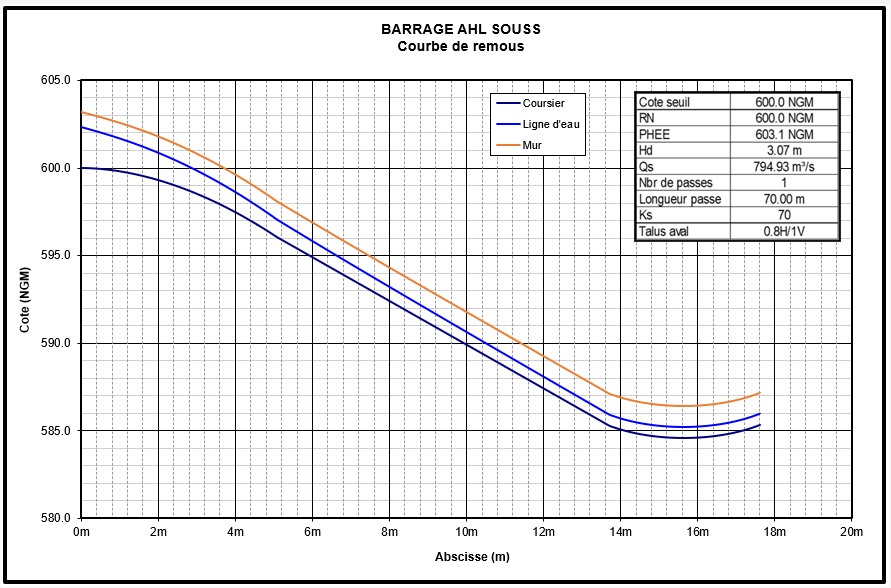
\includegraphics[width=\textwidth]{figures/courbe_remous.png}
    \caption{Courbe de remous — profil de la ligne d'eau le long du coursier pour $Q_{1\,000} = 794{,}93$ m³/s}
    \label{fig:ann2_courbe_remous_q1000}
\end{figure}


% --- BIBLIOGRAPHIE ---
\clearpage
\phantomsection
\addcontentsline{toc}{part}{BIBLIOGRAPHIE}
\printbibliography[heading=none]

\end{document}
